% Options for packages loaded elsewhere
\PassOptionsToPackage{unicode}{hyperref}
\PassOptionsToPackage{hyphens}{url}
\PassOptionsToPackage{dvipsnames,svgnames,x11names}{xcolor}
%
\documentclass[
]{scrartcl}

\usepackage{amsmath,amssymb}
\usepackage{iftex}
\ifPDFTeX
  \usepackage[T1]{fontenc}
  \usepackage[utf8]{inputenc}
  \usepackage{textcomp} % provide euro and other symbols
\else % if luatex or xetex
  \usepackage{unicode-math}
  \defaultfontfeatures{Scale=MatchLowercase}
  \defaultfontfeatures[\rmfamily]{Ligatures=TeX,Scale=1}
\fi
\usepackage{lmodern}
\ifPDFTeX\else  
    % xetex/luatex font selection
    \setmainfont[]{Latin Modern Sans}
    \setsansfont[]{Latin Modern Sans}
\fi
% Use upquote if available, for straight quotes in verbatim environments
\IfFileExists{upquote.sty}{\usepackage{upquote}}{}
\IfFileExists{microtype.sty}{% use microtype if available
  \usepackage[]{microtype}
  \UseMicrotypeSet[protrusion]{basicmath} % disable protrusion for tt fonts
}{}
\makeatletter
\@ifundefined{KOMAClassName}{% if non-KOMA class
  \IfFileExists{parskip.sty}{%
    \usepackage{parskip}
  }{% else
    \setlength{\parindent}{0pt}
    \setlength{\parskip}{6pt plus 2pt minus 1pt}}
}{% if KOMA class
  \KOMAoptions{parskip=half}}
\makeatother
\usepackage{xcolor}
\setlength{\emergencystretch}{3em} % prevent overfull lines
\setcounter{secnumdepth}{5}
% Make \paragraph and \subparagraph free-standing
\makeatletter
\ifx\paragraph\undefined\else
  \let\oldparagraph\paragraph
  \renewcommand{\paragraph}{
    \@ifstar
      \xxxParagraphStar
      \xxxParagraphNoStar
  }
  \newcommand{\xxxParagraphStar}[1]{\oldparagraph*{#1}\mbox{}}
  \newcommand{\xxxParagraphNoStar}[1]{\oldparagraph{#1}\mbox{}}
\fi
\ifx\subparagraph\undefined\else
  \let\oldsubparagraph\subparagraph
  \renewcommand{\subparagraph}{
    \@ifstar
      \xxxSubParagraphStar
      \xxxSubParagraphNoStar
  }
  \newcommand{\xxxSubParagraphStar}[1]{\oldsubparagraph*{#1}\mbox{}}
  \newcommand{\xxxSubParagraphNoStar}[1]{\oldsubparagraph{#1}\mbox{}}
\fi
\makeatother


\providecommand{\tightlist}{%
  \setlength{\itemsep}{0pt}\setlength{\parskip}{0pt}}\usepackage{longtable,booktabs,array}
\usepackage{calc} % for calculating minipage widths
% Correct order of tables after \paragraph or \subparagraph
\usepackage{etoolbox}
\makeatletter
\patchcmd\longtable{\par}{\if@noskipsec\mbox{}\fi\par}{}{}
\makeatother
% Allow footnotes in longtable head/foot
\IfFileExists{footnotehyper.sty}{\usepackage{footnotehyper}}{\usepackage{footnote}}
\makesavenoteenv{longtable}
\usepackage{graphicx}
\makeatletter
\def\maxwidth{\ifdim\Gin@nat@width>\linewidth\linewidth\else\Gin@nat@width\fi}
\def\maxheight{\ifdim\Gin@nat@height>\textheight\textheight\else\Gin@nat@height\fi}
\makeatother
% Scale images if necessary, so that they will not overflow the page
% margins by default, and it is still possible to overwrite the defaults
% using explicit options in \includegraphics[width, height, ...]{}
\setkeys{Gin}{width=\maxwidth,height=\maxheight,keepaspectratio}
% Set default figure placement to htbp
\makeatletter
\def\fps@figure{htbp}
\makeatother
% definitions for citeproc citations
\NewDocumentCommand\citeproctext{}{}
\NewDocumentCommand\citeproc{mm}{%
  \begingroup\def\citeproctext{#2}\cite{#1}\endgroup}
\makeatletter
 % allow citations to break across lines
 \let\@cite@ofmt\@firstofone
 % avoid brackets around text for \cite:
 \def\@biblabel#1{}
 \def\@cite#1#2{{#1\if@tempswa , #2\fi}}
\makeatother
\newlength{\cslhangindent}
\setlength{\cslhangindent}{1.5em}
\newlength{\csllabelwidth}
\setlength{\csllabelwidth}{3em}
\newenvironment{CSLReferences}[2] % #1 hanging-indent, #2 entry-spacing
 {\begin{list}{}{%
  \setlength{\itemindent}{0pt}
  \setlength{\leftmargin}{0pt}
  \setlength{\parsep}{0pt}
  % turn on hanging indent if param 1 is 1
  \ifodd #1
   \setlength{\leftmargin}{\cslhangindent}
   \setlength{\itemindent}{-1\cslhangindent}
  \fi
  % set entry spacing
  \setlength{\itemsep}{#2\baselineskip}}}
 {\end{list}}
\usepackage{calc}
\newcommand{\CSLBlock}[1]{\hfill\break\parbox[t]{\linewidth}{\strut\ignorespaces#1\strut}}
\newcommand{\CSLLeftMargin}[1]{\parbox[t]{\csllabelwidth}{\strut#1\strut}}
\newcommand{\CSLRightInline}[1]{\parbox[t]{\linewidth - \csllabelwidth}{\strut#1\strut}}
\newcommand{\CSLIndent}[1]{\hspace{\cslhangindent}#1}

\usepackage{hyphenat}
\usepackage{graphicx}
% and their extensions so you won't have to specify these with
 % every instance of \includegraphics
\usepackage{pdfcomment}
\DeclareGraphicsExtensions{.pdf,.jpeg,.png}
\usepackage{wallpaper} % for the background image on title page
\usepackage{geometry}
\usepackage{lastpage}
% set font

\usepackage{lmodern}
\usepackage[T1]{fontenc}

\newfontfamily\sectionfont[Color=Black]{Latin Modern Sans}
\newfontfamily\subsectionfont[Color=Black]{Latin Modern Sans}
\newfontfamily\subsubsectionfont[Color=Black]{Latin Modern Sans}

\usepackage[headsepline=0.005pt:,footsepline=0.005pt:,plainfootsepline,automark]{scrlayer-scrpage}
\clearpairofpagestyles
\ohead[]{\headmark} \cofoot[\pagemark]{\pagemark}
\lohead{Yelloweye Rockfish assessment 2025}
\ModifyLayer[addvoffset=-.6ex]{scrheadings.foot.above.line}
\ModifyLayer[addvoffset=-.6ex]{plain.scrheadings.foot.above.line}
% \setkomafont{pageheadfoot}{\small}
\newfontfamily\headfootfont[Color=Black]{Latin Modern Sans}
% Landscape tables and figures
\usepackage{pdflscape}
\newcommand{\blandscape}{\begin{landscape}}
\newcommand{\elandscape}{\end{landscape}}

% Acronyms
\usepackage[acronym]{glossaries}
\glsdisablehyper
\makenoidxglossaries
\loadglsentries{sa4ss_glossaries.tex}
\usepackage{booktabs}
\usepackage{longtable}
\usepackage{array}
\usepackage{multirow}
\usepackage{wrapfig}
\usepackage{float}
\usepackage{colortbl}
\usepackage{pdflscape}
\usepackage{tabu}
\usepackage{threeparttable}
\usepackage{threeparttablex}
\usepackage[normalem]{ulem}
\usepackage{makecell}
\usepackage{xcolor}
\usepackage{caption}
\usepackage{anyfontsize}
\makeatletter
\@ifpackageloaded{caption}{}{\usepackage{caption}}
\AtBeginDocument{%
\ifdefined\contentsname
  \renewcommand*\contentsname{Table of contents}
\else
  \newcommand\contentsname{Table of contents}
\fi
\ifdefined\listfigurename
  \renewcommand*\listfigurename{List of Figures}
\else
  \newcommand\listfigurename{List of Figures}
\fi
\ifdefined\listtablename
  \renewcommand*\listtablename{List of Tables}
\else
  \newcommand\listtablename{List of Tables}
\fi
\ifdefined\figurename
  \renewcommand*\figurename{Figure}
\else
  \newcommand\figurename{Figure}
\fi
\ifdefined\tablename
  \renewcommand*\tablename{Table}
\else
  \newcommand\tablename{Table}
\fi
}
\@ifpackageloaded{float}{}{\usepackage{float}}
\floatstyle{ruled}
\@ifundefined{c@chapter}{\newfloat{codelisting}{h}{lop}}{\newfloat{codelisting}{h}{lop}[chapter]}
\floatname{codelisting}{Listing}
\newcommand*\listoflistings{\listof{codelisting}{List of Listings}}
\makeatother
\makeatletter
\makeatother
\makeatletter
\@ifpackageloaded{caption}{}{\usepackage{caption}}
\@ifpackageloaded{subcaption}{}{\usepackage{subcaption}}
\makeatother

\ifLuaTeX
\usepackage[bidi=basic]{babel}
\else
\usepackage[bidi=default]{babel}
\fi
\babelprovide[main,import]{english}
\ifPDFTeX
\else
\babelfont{rm}[]{Latin Modern Sans}
\fi
% get rid of language-specific shorthands (see #6817):
\let\LanguageShortHands\languageshorthands
\def\languageshorthands#1{}
\ifLuaTeX
  \usepackage{selnolig}  % disable illegal ligatures
\fi
\usepackage{bookmark}

\IfFileExists{xurl.sty}{\usepackage{xurl}}{} % add URL line breaks if available
\urlstyle{same} % disable monospaced font for URLs
\hypersetup{
  pdftitle={Status of Yelloweye Rockfish off the U.S. West Coast in 2025},
  pdfauthor={Morgan A. Johnston*; R. Claire Rosemond*; Alison Whitman; Elizabeth Perl; Matheus de Barros; Juliette Champagnat; Abby Schamp; Samantha Schiano; Fabio Prior Caltabellotta; Vladlena Gertseva; Ian Taylor; Kiva Oken; Aaron Berger},
  pdflang={en},
  colorlinks=true,
  linkcolor={blue},
  filecolor={Maroon},
  citecolor={Blue},
  urlcolor={Blue},
  pdfcreator={LaTeX via pandoc}}


\title{Status of Yelloweye Rockfish off the U.S. West Coast in 2025}
\author{Morgan A. Johnston* \and R. Claire Rosemond* \and Alison
Whitman \and Elizabeth Perl \and Matheus de Barros \and Juliette
Champagnat \and Abby Schamp \and Samantha Schiano \and Fabio Prior
Caltabellotta \and Vladlena Gertseva \and Ian Taylor \and Kiva
Oken \and Aaron Berger}
\date{2025-06-04}

\begin{document}
  \begin{titlepage}
  % This is a combination of Pandoc templating and LaTeX
  % Pandoc templating https://pandoc.org/MANUAL.html#templates
  % See the README for help

  \newgeometry{top=2in,bottom=1in,right=1in,left=1in}
  \begin{minipage}[b][\textheight][s]{\textwidth}
  % Ross would've subbed lines 6, 8 with these lines:
  %\newgeometry{top=2in,bottom=1in,right=1in,left=1in}%
  %\noindent  %\tracingall
  %\begin{minipage}[b][\textheight][s]{.975\textwidth}%% RRM: avoid Overfull box


  \raggedright

  % \includegraphics[width=2cm]{NOAA_Transparent_Logo.png}

  % background image


  % Title and subtitle
  {\huge\bfseries\nohyphens{Status of Yelloweye Rockfish off the U.S.
  West Coast in 2025}}\\[1\baselineskip]
  % Ross would change the end of the above line to the following because \par must come before the group closes and line-depth reverts.
  % }\par}%\\[1\baselineskip]



  \vspace{1\baselineskip}
  % Ross would change this to 2\baselineskip

  %%%%%% Cover image
  \pdftooltip{\includegraphics[width=5in]{support\_files/Yelloweye\_Rockfish.png}}{An illustration of Yelloweye Rockfish}
  % cover page customization need to be inserted here
  %\pdftooltip{\includegraphics{support\_files/Yelloweye\_Rockfish.png}}{Alt text}

  \vspace{1\baselineskip}

  % Authors
  % This hairy bit of code is just to get "and" between the last 2
  % authors. See below if you don't need that
   {\large{Morgan A. Johnston*}}{\textsuperscript{1}}%
  %
  ,
   {\large{R. Claire Rosemond*}}{\textsuperscript{2}}%
  %
  ,
   {\large{Alison Whitman}}{\textsuperscript{3}}%
  %
  ,
   {\large{Elizabeth Perl}}{\textsuperscript{4}}%
  %
  ,
   {\large{Matheus de Barros}}{\textsuperscript{5}}%
  %
  ,
   {\large{Juliette Champagnat}}{\textsuperscript{5}}%
  %
  ,
   {\large{Abby Schamp}}{\textsuperscript{5}}%
  %
  ,
   {\large{Samantha Schiano}}{\textsuperscript{4}}%
  %
  ,
   {\large{Fabio Prior Caltabellotta}}{\textsuperscript{6}}%
  %
  ,
   {\large{Vladlena Gertseva}}{\textsuperscript{7}}%
  %
  ,
   {\large{Ian Taylor}}{\textsuperscript{7}}%
  %
  ,
   {\large{Kiva Oken}}{\textsuperscript{7}}%
  %
  %
  { and \large{Aaron Berger}}%
  {\textsuperscript{2}}%
  %


  % This is how to do it if you don't need the "and"

  %%%%%% Affiliations
  \vspace{2\baselineskip}

  \hangindent=1em
  \hangafter=1
  % Ross would change the above line to:
  % \hangafter=1\relax
  %
  {1}.~{Oregon State University}%
  %
  %
  % Ross recommends putting address on one line
  , %
  {1500 SW Jefferson Way, Corvallis, OR, 97331}%
  %
  \par\hangindent=1em\hangafter=1%
  %
  {2}.~{NOAA Fisheries Northwest Fisheries Science Center}%
  %
  %
  % Ross recommends putting address on one line
  , %
  {2032 SE OSU Drive Building 955, Newport, OR, 97365}%
  %
  \par\hangindent=1em\hangafter=1%
  %
  {3}.~{Oregon Department of Fish and Wildlife}%
  %
  %
  % Ross recommends putting address on one line
  , %
  {2040 SE Marine Science Drive, Newport, OR, 97365}%
  %
  \par\hangindent=1em\hangafter=1%
  %
  {4}.~{ECS Federal in support of NMFS OST}%
  %
  %
  % Ross recommends putting address on one line
  , %
  {East-West Hwy, Silver Spring, MD, 22031}%
  %
  \par\hangindent=1em\hangafter=1%
  %
  {5}.~{University of Washington}%
  %
  %
  % Ross recommends putting address on one line
  , %
  {1410 NE Campus Pkwy, Seattle, WA, 98195}%
  %
  \par\hangindent=1em\hangafter=1%
  %
  {6}.~{Washington Department of Fish and Wildlife}%
  %
  %
  % Ross recommends putting address on one line
  , %
  {1111 Washington St SE, Olympia, WA, 98504}%
  %
  \par\hangindent=1em\hangafter=1%
  %
  {7}.~{NOAA Fisheries Northwest Fisheries Science Center}%
  %
  %
  % Ross recommends putting address on one line
  , %
  {2725 Montlake Boulevard East, Seattle, WA, 98112}%
  %


  %%%%%% Correspondence
  \vspace{1\baselineskip}


  %use \vfill instead to get the space to fill flexibly
  %\vspace{0.25\textheight} % Whitespace between the title block and the publisher

  \vfill


  % Whitespace between the title block and the tagline
  \vspace{1\baselineskip}

  %%%%%% Tagline at bottom
  % Ross says the tagline below could also be centered
  
\includegraphics[alt={},width=2cm]{support_files/us_doc_logo.png}\newline % empty curly brackets without alt text is suitable for this logo because it's purely decorative/an "artifact"
  U.S. Department of Commerce\newline
  National Oceanic and Atmospheric Administration\newline
  National Marine Fisheries Service\newline
  Northwest Fisheries Science Center\newline

  \end{minipage}
  \restoregeometry
  \end{titlepage}

\renewcommand*\contentsname{Table of contents}
{
\hypersetup{linkcolor=}
\setcounter{tocdepth}{3}
\tableofcontents
}

\pagenumbering{roman}
\setcounter{page}{1}

\renewcommand{\thetable}{\roman{table}}
\renewcommand{\thefigure}{\roman{figure}}

\newpage{}

Please cite this publication as:

Johnston*, M. A., Rosemond*, R. C., Whitman, A., Perl, E., Barros, M.,
Champagnat, J., Schamp, A., Schiano, S., Prior Caltabellotta, F.,
Gertseva, V., Taylor, I., Oken, K. and Berger, A. (2025) Status of
Yelloweye rockfish off the U.S. West Coast in 2025. Pacific Fishery
Management Council. \pageref*{LastPage}{} pp.

*These authors contributed equally to this work.

\newpage{}

\pagenumbering{roman}
\setcounter{page}{1}

\renewcommand{\thetable}{\roman{table}}
\renewcommand{\thefigure}{\roman{figure}}

\section*{Disclaimer}\label{disclaimer}
\addcontentsline{toc}{section}{Disclaimer}

These materials do not constitute a formal publication and are for
information only. They are in a pre-review, pre-decisional state and
should not be formally cited or reproduced. They are to be considered
provisional and do not represent any determination or policy of NOAA or
the Department of Commerce.

\newpage{}

\begin{verbatim}
$SS_version
[1] "3.30.23.2;_safe;_compile_date:_Apr 17 2025;_Stock_Synthesis_by_Richard_Methot_(NOAA)_using_ADMB_13.2"

$SS_versionshort
[1] "3.30"

$SS_versionNumeric
[1] 3.3

$StartTime
[1] "StartTime: Thu May 29 17:06:30 2025"

$RunTime
[1] "0 hours, 21 minutes, 32 seconds."

$Files_used
[1] "Data_File: yelloweye_data.ss Control_File: yelloweye_control.ss"

$log_det_hessian
[1] 605.778

$Final_phase
[1] 8

$N_iterations
[1] 1427

$Nwarnings
[1] 7

$warnings
[1] "Note 1 Information: Max data length bin: 74  < max pop len bins: 88; so will accumulate larger pop len bins"                                               
[2] "Note 2 Suggestion:  recr_dist_method 3 is simpler and takes 1 parm for each settlement"                                                                    
[3] "Warning 1 : At least one block pattern ends in endyr. Check the output parameter value time series to see if the values in forecast years are as intended."
[4] "Warning 2 : Minimum pop size bin:_8; is > L at Amin for sex: 1; Gpat: 1; L= 1.54445"                                                                       
[5] "Warning 3 : Final gradient: 0.000557096 is larger than final_conv: 0.0001"                                                                                 
[6] "Note 3 Information:  N parameters that are on or within 1% of min-max bound: 1; check results, variance may be suspect"                                    
[7] " 3 warnings  and 3 notes "                                                                                                                                 

$likelihoods_used
                                            values lambdas
TOTAL                                7874.77000000      NA
Equil_catch                             0.00000000      NA
Survey                                -54.70650000      NA
Length_comp                          1387.28000000      NA
Age_comp                             6526.61000000      NA
Recruitment                            15.32860000    1.00
InitEQ_Regime                           0.00000000    1.00
Forecast_Recruitment                    0.00000000    1.00
Parm_priors                             0.00000000    1.00
Parm_softbounds                         0.00895664      NA
Parm_devs                               0.00000000    1.00
F_Ballpark                              0.24034500    1.00
F_Ballpark(info_only)_1999_estF_tgtF    0.09937910    0.09
Crash_Pen                               0.00000000    1.00

$likelihoods_laplace
                                      values lambdas
NoBias_corr_Recruitment(info_only)  -55.9794       1
Laplace_obj_fun(info_only)         7803.4600      NA

$likelihoods_by_fleet
              Label       ALL 1_CA_TWL 2_CA_NONTWL  3_CA_REC 4_ORWA_TWL
212 Init_equ_lambda        NA    1.000      1.0000   1.00000     1.0000
213   Init_equ_like    0.0000    0.000      0.0000   0.00000     0.0000
214     Surv_lambda        NA    0.000      0.0000   1.00000     0.0000
215       Surv_like  -54.7065    0.000      0.0000  -4.80443     0.0000
216      Surv_N_use        NA    0.000      0.0000  15.00000     0.0000
217     Surv_N_skip        NA    0.000      0.0000   0.00000     0.0000
218   Length_lambda        NA    1.000      1.0000   1.00000     1.0000
219     Length_like 1387.2800  138.497     92.3355 263.67700    82.2725
220    Length_N_use        NA   38.000     44.0000  42.00000    29.0000
221   Length_N_skip        NA    0.000      0.0000   0.00000     0.0000
222      Age_lambda        NA    0.000      1.0000   1.00000     1.0000
223        Age_like 6526.6100    0.000    126.2710 334.85200  1602.6000
224       Age_N_use        NA    0.000     42.0000 102.00000   353.0000
225      Age_N_skip        NA    0.000     10.0000  16.00000    23.0000
    5_ORWA_NONTWL 6_OR_REC  7_WA_REC  8_CACPFV 9_OR_RECOB 10_TRI_ORWA
212        1.0000    1.000   1.00000   1.00000     1.0000     1.00000
213        0.0000    0.000   0.00000   0.00000     0.0000     0.00000
214        0.0000    1.000   1.00000   1.00000     1.0000     1.00000
215        0.0000  -29.243  -5.70765  -6.40195    -4.6242    -1.11697
216        0.0000   36.000  20.00000  11.00000    17.0000     9.00000
217        0.0000    0.000   0.00000   0.00000     0.0000     0.00000
218        1.0000    1.000   1.00000   1.00000     1.0000     1.00000
219       90.7785  181.749 118.28900 165.46000   106.5500    26.75160
220       31.0000   43.000  26.00000  32.00000    20.0000     7.00000
221        0.0000    0.000   0.00000   0.00000     0.0000     0.00000
222        1.0000    1.000   1.00000   0.00000     0.0000     0.00000
223      433.4050 1007.150 808.61000   0.00000     0.0000     0.00000
224      266.0000  195.000 177.00000   0.00000     0.0000     0.00000
225       23.0000   16.000  20.00000   0.00000     0.0000     0.00000
    11_NWFSC_ORWA 12_IPHC_ORWA
212       1.00000      1.00000
213       0.00000      0.00000
214       1.00000      1.00000
215      -5.57326      2.76502
216      21.00000     21.00000
217       0.00000      0.00000
218       1.00000      1.00000
219      66.09200     54.82920
220      21.00000     21.00000
221       0.00000      0.00000
222       1.00000      1.00000
223    1370.26000    843.47400
224     382.00000    531.00000
225      21.00000     36.00000

$N_estimated_parameters
[1] 201

$table_of_phases

-99 -50  -6  -5  -4  -3  -2  -1   1   2   3   4   5   6   7   8 
  1  10   2  31  11   1   1   8   3   2   3  20  10   2 136  25 

$estimated_non_dev_parameters
                                           Value Phase    Min   Max       Init
L_at_Amin_Fem_GP_1                     1.5481500     2   0.01  35.0  1.5444500
L_at_Amax_Fem_GP_1                    61.3623000     2  40.00 120.0 61.3664000
VonBert_K_Fem_GP_1                     0.0759256     1   0.01   0.2  0.0759253
CV_young_Fem_GP_1                      0.1478850     3   0.01   0.5  0.1479200
CV_old_Fem_GP_1                        0.0644086     7   0.01   0.5  0.0643925
RecrDist_Area_2                        0.4729680     3  -4.00   4.0  0.4723950
SR_LN(R0)                              5.4884700     3   3.00  15.0  5.4881300
Impl_err_2025                          0.0000000     8  -1.00   1.0  0.0000000
Impl_err_2026                          0.0000000     8  -1.00   1.0  0.0000000
Impl_err_2027                          0.0000000     8  -1.00   1.0  0.0000000
Impl_err_2028                          0.0000000     8  -1.00   1.0  0.0000000
Impl_err_2029                          0.0000000     8  -1.00   1.0  0.0000000
Impl_err_2030                          0.0000000     8  -1.00   1.0  0.0000000
Impl_err_2031                          0.0000000     8  -1.00   1.0  0.0000000
Impl_err_2032                          0.0000000     8  -1.00   1.0  0.0000000
Impl_err_2033                          0.0000000     8  -1.00   1.0  0.0000000
Impl_err_2034                          0.0000000     8  -1.00   1.0  0.0000000
Impl_err_2035                          0.0000000     8  -1.00   1.0  0.0000000
Impl_err_2036                          0.0000000     8  -1.00   1.0  0.0000000
Q_extraSD_3_CA_REC(3)                  0.1219540     5   0.00   5.0  0.1219990
LnQ_base_6_OR_REC(6)                  -9.1355500     1 -15.00  15.0 -9.1338100
Q_extraSD_6_OR_REC(6)                  0.0841759     5   0.00   5.0  0.0841554
Q_extraSD_7_WA_REC(7)                  0.3830820     5   0.00   5.0  0.3835360
Q_extraSD_8_CACPFV(8)                  0.0965565     5   0.00   5.0  0.0965383
Q_extraSD_9_OR_RECOB(9)                0.1648510     5   0.00   5.0  0.1648590
Q_extraSD_10_TRI_ORWA(10)              0.1399160     5   0.00   5.0  0.1395990
Q_extraSD_12_IPHC_ORWA(12)             0.5517640     5   0.00   5.0  0.5519040
LnQ_base_6_OR_REC(6)_BLK2add_2004     -2.6651000     1  -4.00   4.0 -2.6650500
Size_DblN_peak_1_CA_TWL(1)            43.9644000     4  20.00  60.0 43.9648000
Size_DblN_ascend_se_1_CA_TWL(1)        5.1259700     4  -1.00   9.0  5.1259600
Size_DblN_descend_se_1_CA_TWL(1)      18.2823000     5  -1.00  30.0 18.2831000
Size_DblN_peak_2_CA_NONTWL(2)         44.6592000     4  20.00  60.0 44.6725000
Size_DblN_ascend_se_2_CA_NONTWL(2)     5.2012200     4  -1.00   9.0  5.2022300
Size_DblN_descend_se_2_CA_NONTWL(2)   17.3793000     5  -1.00  30.0 17.3791000
Size_DblN_peak_3_CA_REC(3)            41.7138000     4  20.00  60.0 41.7128000
Size_DblN_ascend_se_3_CA_REC(3)        5.2123200     4  -1.00   9.0  5.2121500
Size_DblN_peak_4_ORWA_TWL(4)          41.9268000     4  20.00  60.0 41.9460000
Size_DblN_ascend_se_4_ORWA_TWL(4)      5.4944100     4  -1.00   9.0  5.4956400
Size_DblN_descend_se_4_ORWA_TWL(4)    18.2437000     5  -1.00  30.0 18.2395000
Size_DblN_peak_5_ORWA_NONTWL(5)       50.8721000     4  20.00  60.0 50.8797000
Size_DblN_ascend_se_5_ORWA_NONTWL(5)   5.4394600     4  -1.00   9.0  5.4398500
Size_DblN_peak_6_OR_REC(6)            36.7208000     4  20.00  60.0 36.7290000
Size_DblN_ascend_se_6_OR_REC(6)        4.1422300     4  -1.00   9.0  4.1432000
Size_DblN_peak_7_WA_REC(7)            42.7552000     6  20.00  60.0 42.7628000
Size_DblN_ascend_se_7_WA_REC(7)        4.3165700     6  -1.00   9.0  4.3175100
Size_DblN_peak_9_OR_RECOB(9)          35.1214000     4  20.00  60.0 35.1235000
Size_DblN_ascend_se_9_OR_RECOB(9)      4.6071100     4  -1.00   9.0  4.6072000
Size_DblN_peak_10_TRI_ORWA(10)        79.9716000     4  20.00  80.0 79.9717000
Size_DblN_ascend_se_10_TRI_ORWA(10)    7.0799400     4  -1.00   9.0  7.0795500
Size_DblN_peak_11_NWFSC_ORWA(11)      48.8552000     4  20.00  60.0 48.8733000
Size_DblN_ascend_se_11_NWFSC_ORWA(11)  6.2342700     4  -1.00   9.0  6.2350700
Size_DblN_peak_12_IPHC_ORWA(12)       53.9882000     4  20.00  60.0 53.9958000
Size_DblN_ascend_se_12_IPHC_ORWA(12)   4.1367400     4  -1.00   9.0  4.1375000
                                      Status   Parm_StDev         Gradient
L_at_Amin_Fem_GP_1                        OK   0.58181400 -0.0000237729000
L_at_Amax_Fem_GP_1                        OK   0.22501200 -0.0002569350000
VonBert_K_Fem_GP_1                        OK   0.00132714 -0.0001496400000
CV_young_Fem_GP_1                         OK   0.00676421 -0.0000033617200
CV_old_Fem_GP_1                           OK   0.00193725 -0.0000004034390
RecrDist_Area_2                           OK   0.02350840 -0.0002301870000
SR_LN(R0)                                 OK   0.06084550 -0.0005570950000
Impl_err_2025                            act   0.00010000  0.0000000000000
Impl_err_2026                            act   0.00010000  0.0000000000000
Impl_err_2027                            act   0.00010000  0.0000000000000
Impl_err_2028                            act   0.00010000  0.0000000000000
Impl_err_2029                            act   0.00010000  0.0000000000000
Impl_err_2030                            act   0.00010000  0.0000000000000
Impl_err_2031                            act   0.00010000  0.0000000000000
Impl_err_2032                            act   0.00010000  0.0000000000000
Impl_err_2033                            act   0.00010000  0.0000000000000
Impl_err_2034                            act   0.00010000  0.0000000000000
Impl_err_2035                            act   0.00010000  0.0000000000000
Impl_err_2036                            act   0.00010000  0.0000000000000
Q_extraSD_3_CA_REC(3)                     OK   0.07803440 -0.0000039876400
LnQ_base_6_OR_REC(6)                      OK   0.11091100 -0.0002825200000
Q_extraSD_6_OR_REC(6)                     OK   0.02897510 -0.0000068352100
Q_extraSD_7_WA_REC(7)                     OK   0.07625640 -0.0000108947000
Q_extraSD_8_CACPFV(8)                     OK   0.07456620 -0.0000007525470
Q_extraSD_9_OR_RECOB(9)                   OK   0.07923370 -0.0000029946200
Q_extraSD_10_TRI_ORWA(10)                 OK   0.12188300  0.0000003429160
Q_extraSD_12_IPHC_ORWA(12)                OK   0.10650800  0.0000014280600
LnQ_base_6_OR_REC(6)_BLK2add_2004         OK   0.11159900 -0.0000639063000
Size_DblN_peak_1_CA_TWL(1)                OK   3.30615000  0.0000212362000
Size_DblN_ascend_se_1_CA_TWL(1)           OK   0.40407500 -0.0001125750000
Size_DblN_descend_se_1_CA_TWL(1)          OK 151.70400000  0.0000000352366
Size_DblN_peak_2_CA_NONTWL(2)             OK   2.48523000  0.0000166438000
Size_DblN_ascend_se_2_CA_NONTWL(2)        OK   0.28051500 -0.0000541514000
Size_DblN_descend_se_2_CA_NONTWL(2)       OK 171.44900000  0.0000010886800
Size_DblN_peak_3_CA_REC(3)                OK   1.35482000 -0.0000048134300
Size_DblN_ascend_se_3_CA_REC(3)           OK   0.14373900  0.0000032842300
Size_DblN_peak_4_ORWA_TWL(4)              OK   3.03695000 -0.0000090425500
Size_DblN_ascend_se_4_ORWA_TWL(4)         OK   0.34266600  0.0000271868000
Size_DblN_descend_se_4_ORWA_TWL(4)        OK 152.46900000  0.0000003791700
Size_DblN_peak_5_ORWA_NONTWL(5)           OK   1.47753000 -0.0000126335000
Size_DblN_ascend_se_5_ORWA_NONTWL(5)      OK   0.14656300  0.0000298324000
Size_DblN_peak_6_OR_REC(6)                OK   1.26781000  0.0000178959000
Size_DblN_ascend_se_6_OR_REC(6)           OK   0.27987500 -0.0000140674000
Size_DblN_peak_7_WA_REC(7)                OK   2.75354000 -0.0000000378847
Size_DblN_ascend_se_7_WA_REC(7)           OK   0.51790400 -0.0000057450900
Size_DblN_peak_9_OR_RECOB(9)              OK   1.62843000  0.0000042199500
Size_DblN_ascend_se_9_OR_RECOB(9)         OK   0.29186800 -0.0000057021300
Size_DblN_peak_10_TRI_ORWA(10)            HI   0.89926500  0.0000030834900
Size_DblN_ascend_se_10_TRI_ORWA(10)       OK   0.26425500  0.0000033367000
Size_DblN_peak_11_NWFSC_ORWA(11)          OK   5.59042000 -0.0000027020300
Size_DblN_ascend_se_11_NWFSC_ORWA(11)     OK   0.38642500 -0.0000009594890
Size_DblN_peak_12_IPHC_ORWA(12)           OK   1.21365000 -0.0000124892000
Size_DblN_ascend_se_12_IPHC_ORWA(12)      OK   0.23314600  0.0000136462000
                                       Pr_type Prior Pr_SD Pr_Like Afterbound
L_at_Amin_Fem_GP_1                    No_prior    NA    NA      NA         OK
L_at_Amax_Fem_GP_1                    No_prior    NA    NA      NA         OK
VonBert_K_Fem_GP_1                    No_prior    NA    NA      NA         OK
CV_young_Fem_GP_1                     No_prior    NA    NA      NA         OK
CV_old_Fem_GP_1                       No_prior    NA    NA      NA         OK
RecrDist_Area_2                       No_prior    NA    NA      NA         OK
SR_LN(R0)                             No_prior    NA    NA      NA         OK
Impl_err_2025                              dev    NA    NA      NA         OK
Impl_err_2026                              dev    NA    NA      NA         OK
Impl_err_2027                              dev    NA    NA      NA         OK
Impl_err_2028                              dev    NA    NA      NA         OK
Impl_err_2029                              dev    NA    NA      NA         OK
Impl_err_2030                              dev    NA    NA      NA         OK
Impl_err_2031                              dev    NA    NA      NA         OK
Impl_err_2032                              dev    NA    NA      NA         OK
Impl_err_2033                              dev    NA    NA      NA         OK
Impl_err_2034                              dev    NA    NA      NA         OK
Impl_err_2035                              dev    NA    NA      NA         OK
Impl_err_2036                              dev    NA    NA      NA         OK
Q_extraSD_3_CA_REC(3)                 No_prior    NA    NA      NA         OK
LnQ_base_6_OR_REC(6)                  No_prior    NA    NA      NA         OK
Q_extraSD_6_OR_REC(6)                 No_prior    NA    NA      NA         OK
Q_extraSD_7_WA_REC(7)                 No_prior    NA    NA      NA         OK
Q_extraSD_8_CACPFV(8)                 No_prior    NA    NA      NA         OK
Q_extraSD_9_OR_RECOB(9)               No_prior    NA    NA      NA         OK
Q_extraSD_10_TRI_ORWA(10)             No_prior    NA    NA      NA         OK
Q_extraSD_12_IPHC_ORWA(12)            No_prior    NA    NA      NA         OK
LnQ_base_6_OR_REC(6)_BLK2add_2004     No_prior    NA    NA      NA         OK
Size_DblN_peak_1_CA_TWL(1)            No_prior    NA    NA      NA         OK
Size_DblN_ascend_se_1_CA_TWL(1)       No_prior    NA    NA      NA         OK
Size_DblN_descend_se_1_CA_TWL(1)      No_prior    NA    NA      NA         OK
Size_DblN_peak_2_CA_NONTWL(2)         No_prior    NA    NA      NA         OK
Size_DblN_ascend_se_2_CA_NONTWL(2)    No_prior    NA    NA      NA         OK
Size_DblN_descend_se_2_CA_NONTWL(2)   No_prior    NA    NA      NA         OK
Size_DblN_peak_3_CA_REC(3)            No_prior    NA    NA      NA         OK
Size_DblN_ascend_se_3_CA_REC(3)       No_prior    NA    NA      NA         OK
Size_DblN_peak_4_ORWA_TWL(4)          No_prior    NA    NA      NA         OK
Size_DblN_ascend_se_4_ORWA_TWL(4)     No_prior    NA    NA      NA         OK
Size_DblN_descend_se_4_ORWA_TWL(4)    No_prior    NA    NA      NA         OK
Size_DblN_peak_5_ORWA_NONTWL(5)       No_prior    NA    NA      NA         OK
Size_DblN_ascend_se_5_ORWA_NONTWL(5)  No_prior    NA    NA      NA         OK
Size_DblN_peak_6_OR_REC(6)            No_prior    NA    NA      NA         OK
Size_DblN_ascend_se_6_OR_REC(6)       No_prior    NA    NA      NA         OK
Size_DblN_peak_7_WA_REC(7)            No_prior    NA    NA      NA         OK
Size_DblN_ascend_se_7_WA_REC(7)       No_prior    NA    NA      NA         OK
Size_DblN_peak_9_OR_RECOB(9)          No_prior    NA    NA      NA         OK
Size_DblN_ascend_se_9_OR_RECOB(9)     No_prior    NA    NA      NA         OK
Size_DblN_peak_10_TRI_ORWA(10)        No_prior    NA    NA      NA         OK
Size_DblN_ascend_se_10_TRI_ORWA(10)   No_prior    NA    NA      NA         OK
Size_DblN_peak_11_NWFSC_ORWA(11)      No_prior    NA    NA      NA         OK
Size_DblN_ascend_se_11_NWFSC_ORWA(11) No_prior    NA    NA      NA         OK
Size_DblN_peak_12_IPHC_ORWA(12)       No_prior    NA    NA      NA         OK
Size_DblN_ascend_se_12_IPHC_ORWA(12)  No_prior    NA    NA      NA         OK

$maximum_gradient_component
[1] 0.000557096

$parameters_with_highest_gradients
                          Value     Gradient
SR_LN(R0)             5.4884700 -0.000557095
LnQ_base_6_OR_REC(6) -9.1355500 -0.000282520
L_at_Amax_Fem_GP_1   61.3623000 -0.000256935
RecrDist_Area_2       0.4729680 -0.000230187
VonBert_K_Fem_GP_1    0.0759256 -0.000149640

$Length_Comp_Fit_Summary
     Data_type Fleet Recommend_var_adj #  N Npos min_Nsamp max_Nsamp
5992         4     1          0.507139 # 38   38  0.590901  16.06340
5993         4     2          0.408984 # 44   44  0.652720  50.16200
5994         4     3          0.573071 # 42   42  2.818790  82.43240
5995         4     4          0.583293 # 29   29  1.266840  33.17670
5996         4     5          0.436521 # 31   31  0.953371 104.10000
5997         4     6          0.224556 # 43   43  0.827633 137.15300
5998         4     7          0.504382 # 26   26  1.138000  33.08200
5999         4     8          0.336359 # 32   32  1.911600  64.67290
6000         4     9          0.574334 # 20   20  1.232110  24.46080
6001         4    10          1.295240 #  7    7  1.689720   7.72443
6002         4    11          2.045650 # 21   21  4.078750  13.03360
6003         4    12          2.376180 # 21   21 14.295400  53.18410
     mean_Nsamp_in mean_Nsamp_adj mean_Nsamp_DM err_method err_index
5992       9.93300        5.15766            NA          0        NA
5993      34.92250       10.01520            NA          0        NA
5994      45.84090       24.01780            NA          0        NA
5995      37.23070        9.49766            NA          0        NA
5996      79.26010       29.60980            NA          0        NA
5997      52.47780       19.08280            NA          0        NA
5998       7.25315        7.25315            NA          0        NA
5999      37.58630       21.04570            NA          0        NA
6000      25.59210       13.85430            NA          0        NA
6001      11.24710        5.12251            NA          0        NA
6002      16.07050        8.21397            NA          0        NA
6003      28.71880       25.62720            NA          0        NA
            par1 val1 par2 val2 mean_effN  HarMean Curr_Var_Adj    Fleet_name
5992 multinomial   NA   NA   NA   14.8207  5.03741     0.519245      1_CA_TWL
5993 multinomial   NA   NA   NA   82.6929 14.28270     0.286784   2_CA_NONTWL
5994 multinomial   NA   NA   NA   49.8449 26.27010     0.523939      3_CA_REC
5995 multinomial   NA   NA   NA   58.9380 21.71640     0.255103    4_ORWA_TWL
5996 multinomial   NA   NA   NA  125.7480 34.59870     0.373578 5_ORWA_NONTWL
5997 multinomial   NA   NA   NA   52.7387 11.78420     0.363635      6_OR_REC
5998 multinomial   NA   NA   NA   33.4103  3.65836     1.000000      7_WA_REC
5999 multinomial   NA   NA   NA   54.7114 12.64250     0.559929      8_CACPFV
6000 multinomial   NA   NA   NA   43.0027 14.69840     0.541348    9_OR_RECOB
6001 multinomial   NA   NA   NA   20.3179 14.56770     0.455450   10_TRI_ORWA
6002 multinomial   NA   NA   NA   37.8948 32.87450     0.511122 11_NWFSC_ORWA
6003 multinomial   NA   NA   NA   97.0288 68.24090     0.892350  12_IPHC_ORWA

$Age_Comp_Fit_Summary
     Data_type Fleet Recommend_var_adj # Nsamp_adj Npos min_Nsamp max_Nsamp
8223         5     2          0.972023 #        52   42  1.000000    3.0000
8224         5     3          0.883836 #       118  102  1.000000    6.0000
8225         5     4          0.540511 #       376  353  1.000000   24.0000
8226         5     5          0.290019 #       289  266  0.222147   15.1060
8227         5     6          0.556431 #       211  195  1.000000   16.0000
8228         5     7          0.544391 #       197  177  1.000000   17.0000
8229         5    11          0.760222 #       403  382  1.000000   12.0000
8230         5    12          0.236145 #       567  531  0.088235   10.2353
     mean_Nsamp_in mean_Nsamp_adj mean_Nsamp_DM err_method err_index
8223       1.38095        1.38095            NA          0        NA
8224       1.50000        1.50000            NA          0        NA
8225       4.20963        4.20963            NA          0        NA
8226       8.85714        1.96759            NA          0        NA
8227       4.09231        4.09231            NA          0        NA
8228       3.63277        3.63277            NA          0        NA
8229       2.27749        2.27749            NA          0        NA
8230      15.98310        1.41026            NA          0        NA
            par1 val1 par2 val2 mean_effN HarMean Curr_Var_Adj    Fleet_name
8223 multinomial   NA   NA   NA   1.64940 1.34232     1.000000   2_CA_NONTWL
8224 multinomial   NA   NA   NA   1.94868 1.32575     1.000000      3_CA_REC
8225 multinomial   NA   NA   NA   4.68721 2.27535     1.000000    4_ORWA_TWL
8226 multinomial   NA   NA   NA   8.44498 2.56874     0.222147 5_ORWA_NONTWL
8227 multinomial   NA   NA   NA   4.73156 2.27709     1.000000      6_OR_REC
8228 multinomial   NA   NA   NA   4.48774 1.97765     1.000000      7_WA_REC
8229 multinomial   NA   NA   NA   3.05821 1.73140     1.000000 11_NWFSC_ORWA
8230 multinomial   NA   NA   NA  10.12170 3.77432     0.088235  12_IPHC_ORWA

$SBzero
[1] 594.999

$current_depletion
[1] 0.4013704

$SPRratioLabel
[1] "(1-SPR)/(1-SPR_50%)"

$sigma_R_in
[1] 0.5

$sigma_R_info
           period N_devs SD_of_devs Var_of_devs   mean_SE mean_SEsquared
1            Main     44  0.5827591   0.3396082 0.3609410      0.1356366
2      Early+Main    135  0.3730102   0.1391366 0.4305959      0.1907855
3 Early+Main+Late    136  0.3716374   0.1381143 0.4311062      0.1912209
  sqrt_sum_of_components SD_of_devs_over_sigma_R sqrt_sum_over_sigma_R
1              0.6893800               1.1655183              1.378760
2              0.5743885               0.7460205              1.148777
3              0.5738774               0.7432748              1.147755
  alternative_sigma_R
1   0.689380012630552
2   0.574388519195281
3   0.573877414336972

$rmse_table
    ERA  N     RMSE RMSE_over_sigmaR mean_BiasAdj
1  main 44 0.576099         1.327560     0.459768
2 early 91 0.214696         0.184378     0.130709

$RecDev_method
[1] 1
\end{verbatim}

\begin{verbatim}
[1] "7_WA_REC"
\end{verbatim}

\begin{verbatim}
[1] 2.105
\end{verbatim}

\newpage{}

\markright{Executive Summary}

\section*{Executive Summary}\label{executive-summary}
\addcontentsline{toc}{section}{Executive Summary}

\subsection*{Stock}\label{stock}
\addcontentsline{toc}{subsection}{Stock}

This update assessment reports the status of Yelloweye Rockfish
(\emph{Sebastes ruberrimus}) off the U.S. West Coast using data through
2024. Yelloweye Rockfish are found from the Gulf of Alaska to northern
Baja California in Mexico across the northeastern Pacific Ocean. Their
core distribution is from southeast Alaska to central California on the
west coast of the United States. Yelloweye Rockfish are strongly
associated with rocky bottom habtiat and adults are considered to be
solitary and sedentary after settlement. Given the general perception of
the sedentary nature of Yelloweye Rockfish adults and the moderate
amount of mixing that occurs during the pelagic larval stage, the
previous Yelloweye Rockfish assessment, conducted in 2017, modeled the
West coast population as a two-area assessment (California and a
combined Oregon-Washington area) with a common stock recruitment
relationship. This update assessment necessarily maintains this same
structure.

\subsection*{Catches}\label{catches}
\addcontentsline{toc}{subsection}{Catches}

Catches for Yelloweye Rockfish have averaged over \(20 mt\) in recent
years (Figure~\ref{fig-es-landings}, Table~\ref{tbl-es-catches}). The
Yelloweye Rockfish stock was declared overfished in \(2002\) and remains
under a rebuilding plan that substantially limits catch. However, as
other rockfish stocks have rebuilt and Yelloweye Rockfish has progressed
under its rebuilding plan, catches have slowly increased in recent
years, primarily in the Oregon-Washington non-trawl fleet and the
recreational fleets.

\begin{figure}

\centering{

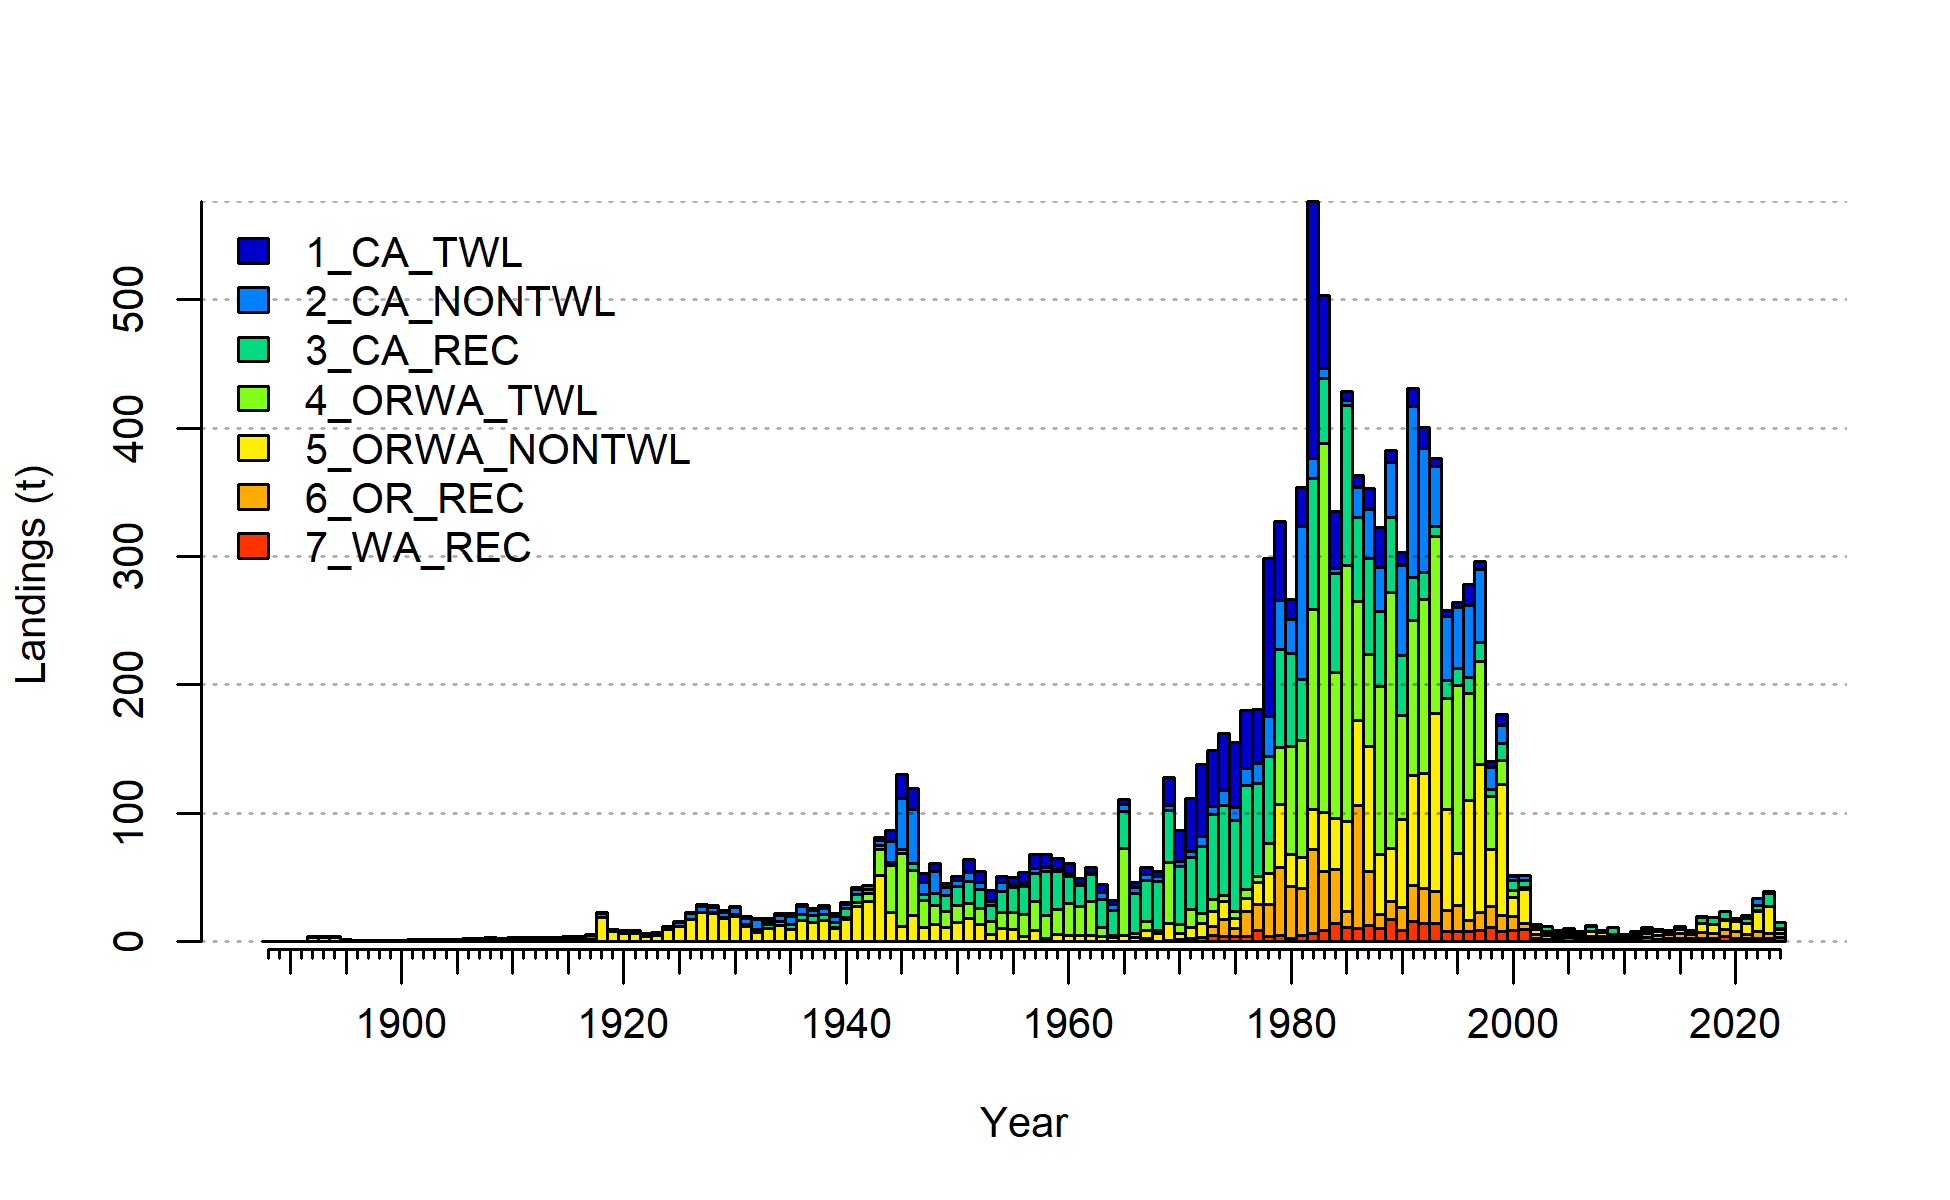
\includegraphics{figures/r4ss_plots/plots/catch2_landings_stacked.png}

}

\caption{\label{fig-es-landings}Yelloweye Rockfish landing history in
metric tons (mt) between 1889 and 2024 for each fleet.}

\end{figure}%

\clearpage

\begin{landscape}
\begingroup
\setlength\LTleft{0.2\linewidth}
\setlength\LTright{0.2\linewidth}\fontsize{9.0pt}{10.8pt}\selectfont

\begin{longtable}{@{\extracolsep{\fill}}rrrrrrrrr}

\caption{\label{tbl-es-catches}Recent catches (mt) by fleet and total
catch (mt) summed across fleets.}

\tabularnewline

\toprule
Year & CA TWL (mt) & CA NONTWL (mt) & CA REC (mt) & ORWA TWL (mt) & ORWA NONTWL (mt) & OR REC (mt) & WA REC (mt) & Catch (mt) \\ 
\midrule\addlinespace[2.5pt]
2015 & 0.00 & 0.40 & 2.00 & 0.03 & 3.15 & 4.26 & 2.10 & 11.94 \\ 
2016 & 0.00 & 0.00 & 1.00 & 0.07 & 2.59 & 2.84 & 2.46 & 8.96 \\ 
2017 & 0.01 & 1.23 & 4.52 & 0.24 & 6.97 & 4.27 & 2.49 & 19.73 \\ 
2018 & 0.00 & 0.00 & 4.99 & 0.54 & 6.38 & 4.01 & 2.57 & 18.49 \\ 
2019 & 0.04 & 0.00 & 6.16 & 0.59 & 7.43 & 5.04 & 4.23 & 23.49 \\ 
2020 & 0.13 & 0.00 & 1.95 & 0.32 & 7.52 & 6.00 & 2.24 & 18.16 \\ 
2021 & 0.12 & 2.43 & 3.96 & 0.39 & 7.97 & 3.34 & 2.54 & 20.75 \\ 
2022 & 0.10 & 5.60 & 3.80 & 0.76 & 15.55 & 5.20 & 2.65 & 33.66 \\ 
2023 & 0.09 & 1.83 & 9.59 & 0.40 & 20.64 & 3.84 & 2.88 & 39.27 \\ 
2024 & 0.19 & 3.27 & 4.65 & 0.49 & 13.51 & 3.66 & 2.92 & 28.69 \\ 
\bottomrule

\end{longtable}

\endgroup

\end{landscape}

\clearpage

\subsection*{Data and Assessment}\label{data-and-assessment}
\addcontentsline{toc}{subsection}{Data and Assessment}

The last assessment for Yelloweye Rockfish occurred in 2017. This update
assessment extends the data used in the 2017 assessment through 2024.
This assessment uses the stock assessment framework Stock Synthesis (SS3
Version 3.30.23.2) by Methot and Wetzel (2013). Data includes catch,
length and age data from seven fishery fleets and multiple indices of
abundance in California and Oregon/Washington. Two new historical catch
reconstructions from Oregon and Washington were incorporated. Four
indices of abundance were updated for this assessment, including two
recreational fishery indices in Oregon, the \gls{indexwc}, and the
\gls{iphc} longline survey. In addition, sample sizes and assignment of
aging error were corrected in the compositional data. No new data
streams were considered in this update assessment.

\subsection*{Stock Spawning Output and
Dynamics}\label{stock-spawning-output-and-dynamics}
\addcontentsline{toc}{subsection}{Stock Spawning Output and Dynamics}

The Yelloweye Rockfish assessment uses estimates of fecundity
(eggs-at-length) from the Dick et al. (2017) method, and spawning output
is reported in millions of eggs. The unexploited level of spawning stock
output is estimated to be 1190 million eggs (95\% confidence interval:
1,048.1 - 1,331.9 million eggs) (Figure~\ref{fig-es-so}). At the
beginning of 2025, the spawning stock output is estimated to be 477.63
million eggs (95\% confidence interval: 384 -- 571 million eggs), which
represents 40.1\% of the unfished spawning output level.

Estimated relative spawning output was below the minimum stock size
threshold in the late 1990s and was lowest in the early 2000s before
increasing over the last 20 years. The 2025 estimated relative spawning
output follows an increasing trajectory and is slightly above the
management target threshold (Figure~\ref{fig-es-so},
Figure~\ref{fig-es-sb}). Though Yelloweye Rockfish are considered a
single stock due to their population's even genetic and spatial
structure throughout their range, this assessment is modeled with two
areas (California and Oregon-Washington). Current population status
differs by area which may be valuable information for making management
and allocation decisions (Figure~\ref{fig-status-area-es}).

\clearpage

\pagebreak

\begingroup
\fontsize{9.0pt}{10.8pt}\selectfont

\begin{longtable}{>{\centering\arraybackslash}p{\dimexpr 56.25pt -2\tabcolsep-1.5\arrayrulewidth}>{\centering\arraybackslash}p{\dimexpr 56.25pt -2\tabcolsep-1.5\arrayrulewidth}>{\centering\arraybackslash}p{\dimexpr 56.25pt -2\tabcolsep-1.5\arrayrulewidth}>{\centering\arraybackslash}p{\dimexpr 56.25pt -2\tabcolsep-1.5\arrayrulewidth}>{\centering\arraybackslash}p{\dimexpr 56.25pt -2\tabcolsep-1.5\arrayrulewidth}>{\centering\arraybackslash}p{\dimexpr 56.25pt -2\tabcolsep-1.5\arrayrulewidth}>{\centering\arraybackslash}p{\dimexpr 56.25pt -2\tabcolsep-1.5\arrayrulewidth}}

\caption{\label{tbl-es-sb}Estimated recent trend in spawning output
(millions of eggs) and the fraction of unfished spawning output and the
95 percent confidence intervals.}

\tabularnewline

\toprule
Year & Spawning output & Lower Interval. & Upper Interval. & Fraction Unfished & Lower Interval & Upper Interval \\ 
\midrule\addlinespace[2.5pt]
2015 & 293.07 & 233.20 & 352.95 & 0.246 & 0.211 & 0.282 \\ 
2016 & 304.71 & 242.84 & 366.58 & 0.256 & 0.220 & 0.293 \\ 
2017 & 317.87 & 253.80 & 381.94 & 0.267 & 0.230 & 0.305 \\ 
2018 & 331.52 & 265.00 & 398.05 & 0.279 & 0.240 & 0.317 \\ 
2019 & 347.17 & 277.86 & 416.48 & 0.292 & 0.252 & 0.332 \\ 
2020 & 364.48 & 292.01 & 436.95 & 0.306 & 0.265 & 0.348 \\ 
2021 & 384.48 & 308.44 & 460.51 & 0.323 & 0.280 & 0.366 \\ 
2022 & 406.33 & 326.37 & 486.28 & 0.341 & 0.296 & 0.387 \\ 
2023 & 428.74 & 344.53 & 512.94 & 0.360 & 0.313 & 0.408 \\ 
2024 & 452.09 & 363.37 & 540.81 & 0.380 & 0.330 & 0.430 \\ 
2025 & 477.63 & 384.18 & 571.08 & 0.401 & 0.349 & 0.453 \\ 
\bottomrule

\end{longtable}

\endgroup

\begin{figure}[H]

\centering{

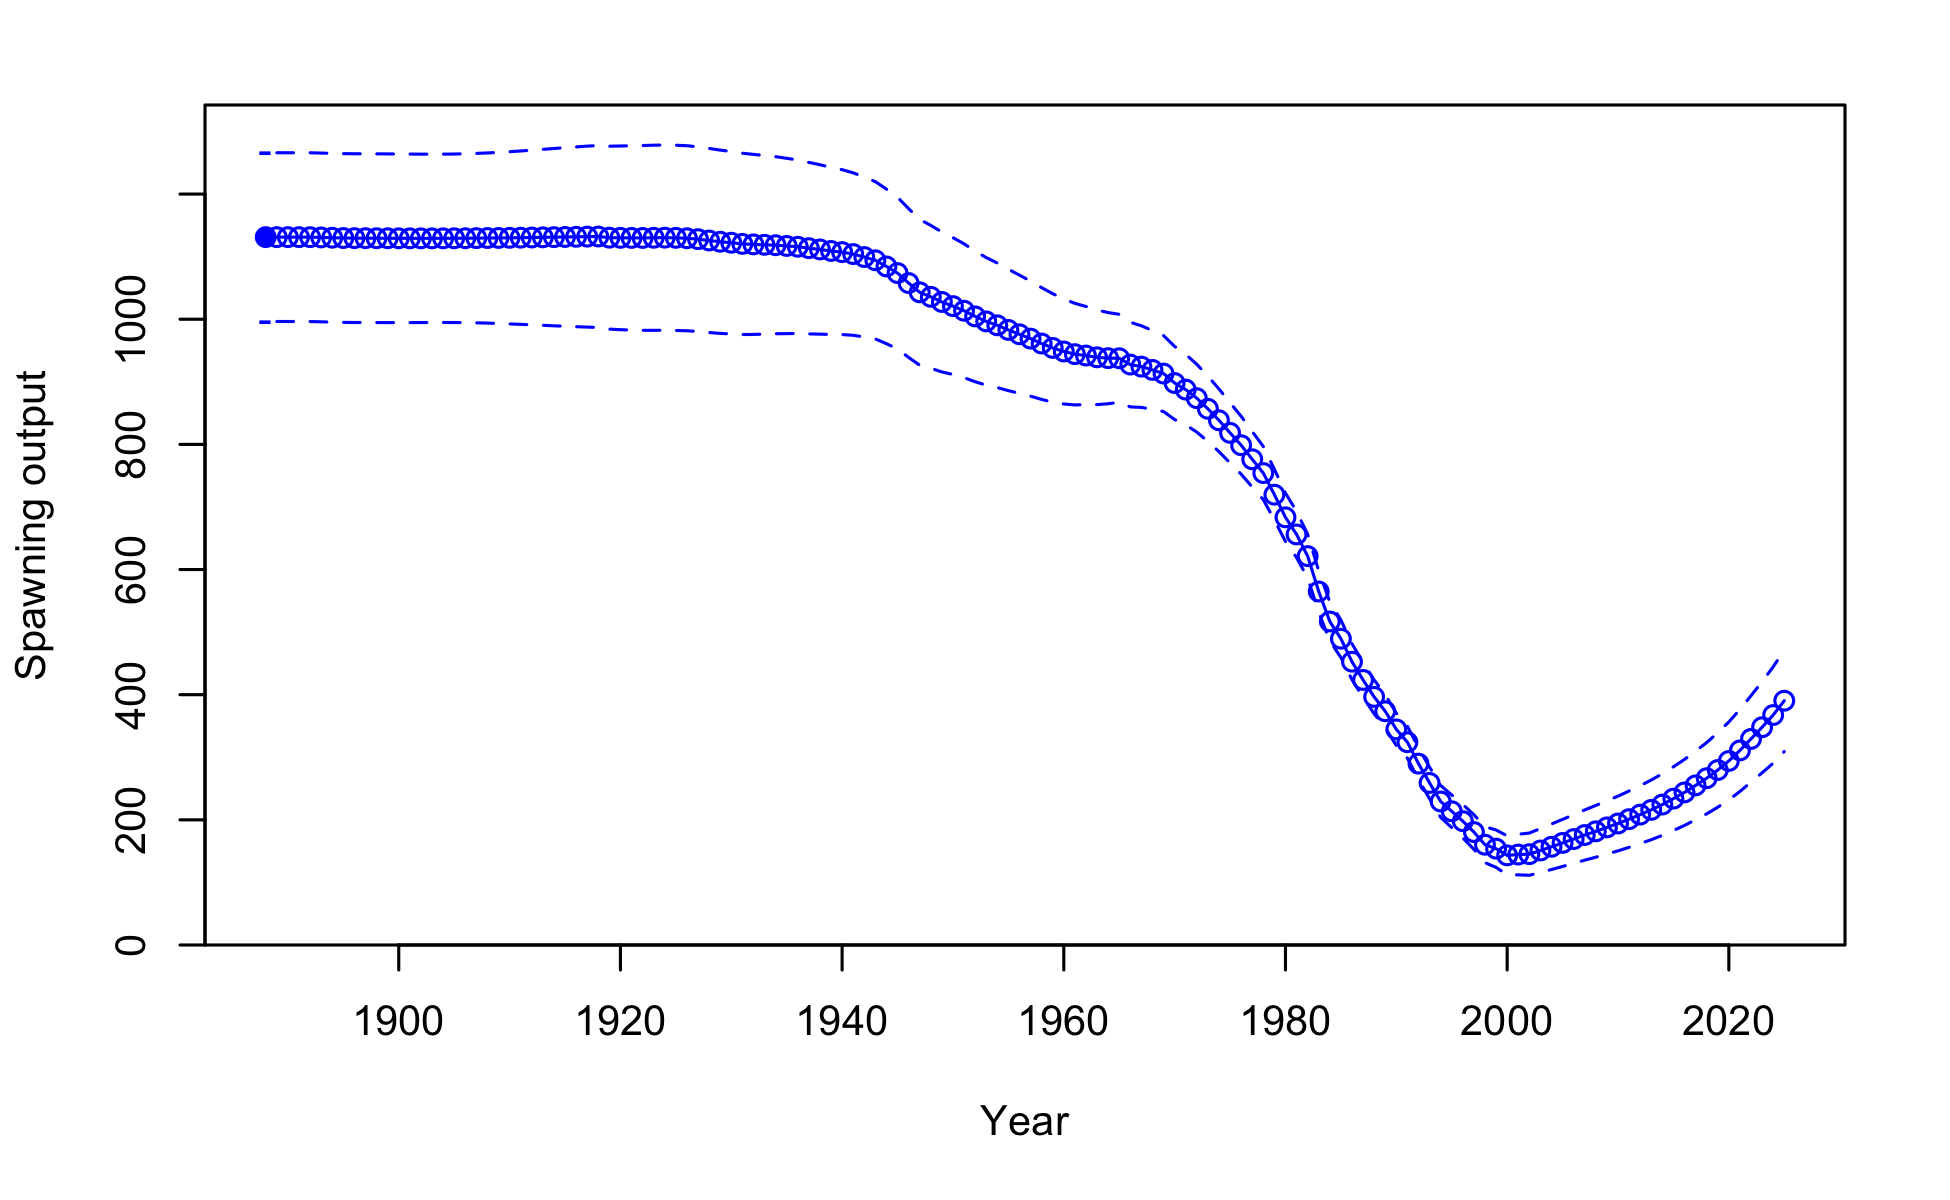
\includegraphics{figures/r4ss_plots/plots/ts7_Spawning_output_with_95_intervals.png}

}

\caption{\label{fig-es-so}Time series of estimated spawning output
(millions of eggs) for the base model (circles) with \textasciitilde{}
95\% interval (dashed lines).}

\end{figure}%

\begin{figure}[H]

\centering{

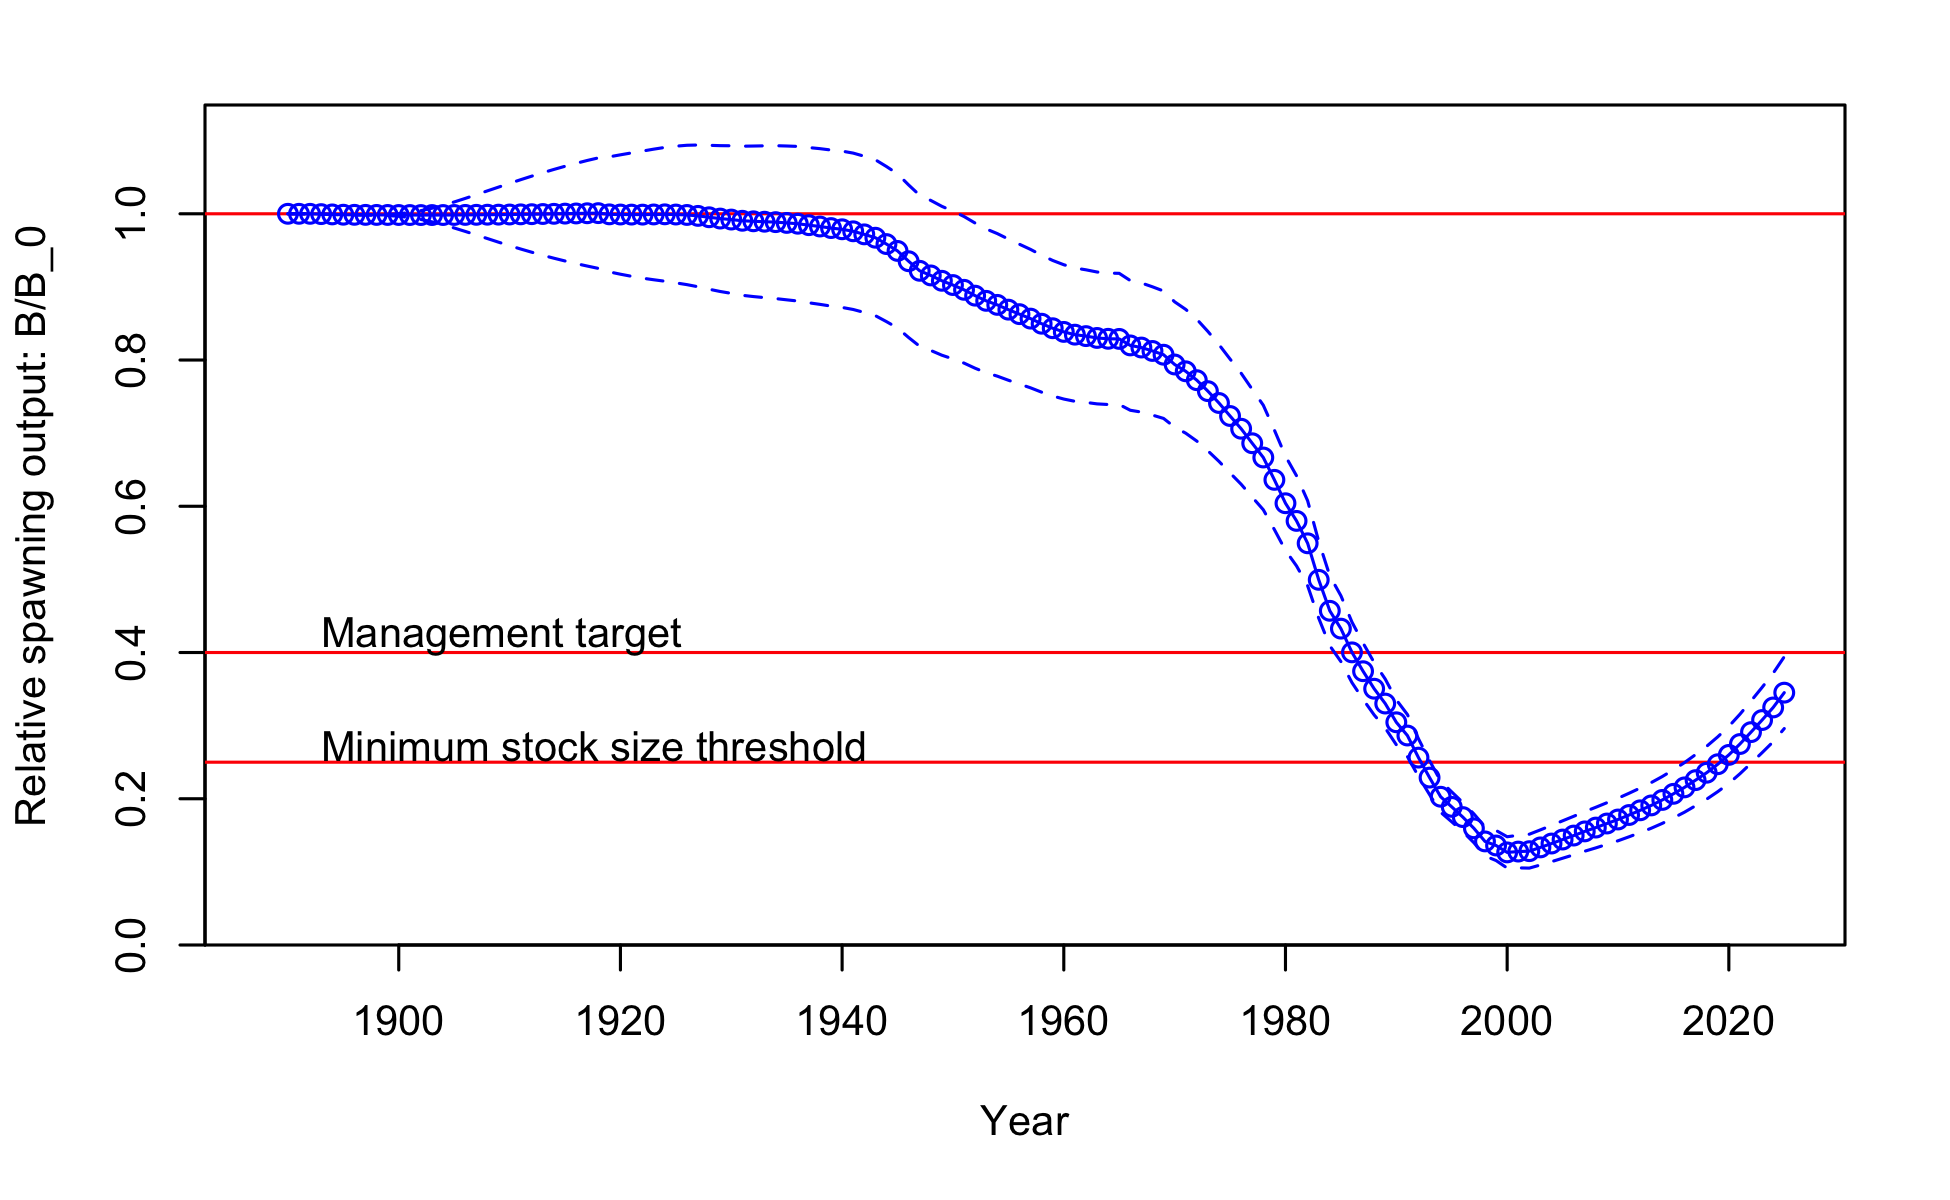
\includegraphics{figures/r4ss_plots/plots/ts9_Relative_spawning_output_intervals.png}

}

\caption{\label{fig-es-sb}Time series of estimated relative spawning
output for the base model.}

\end{figure}%

\begin{figure}[H]

\centering{

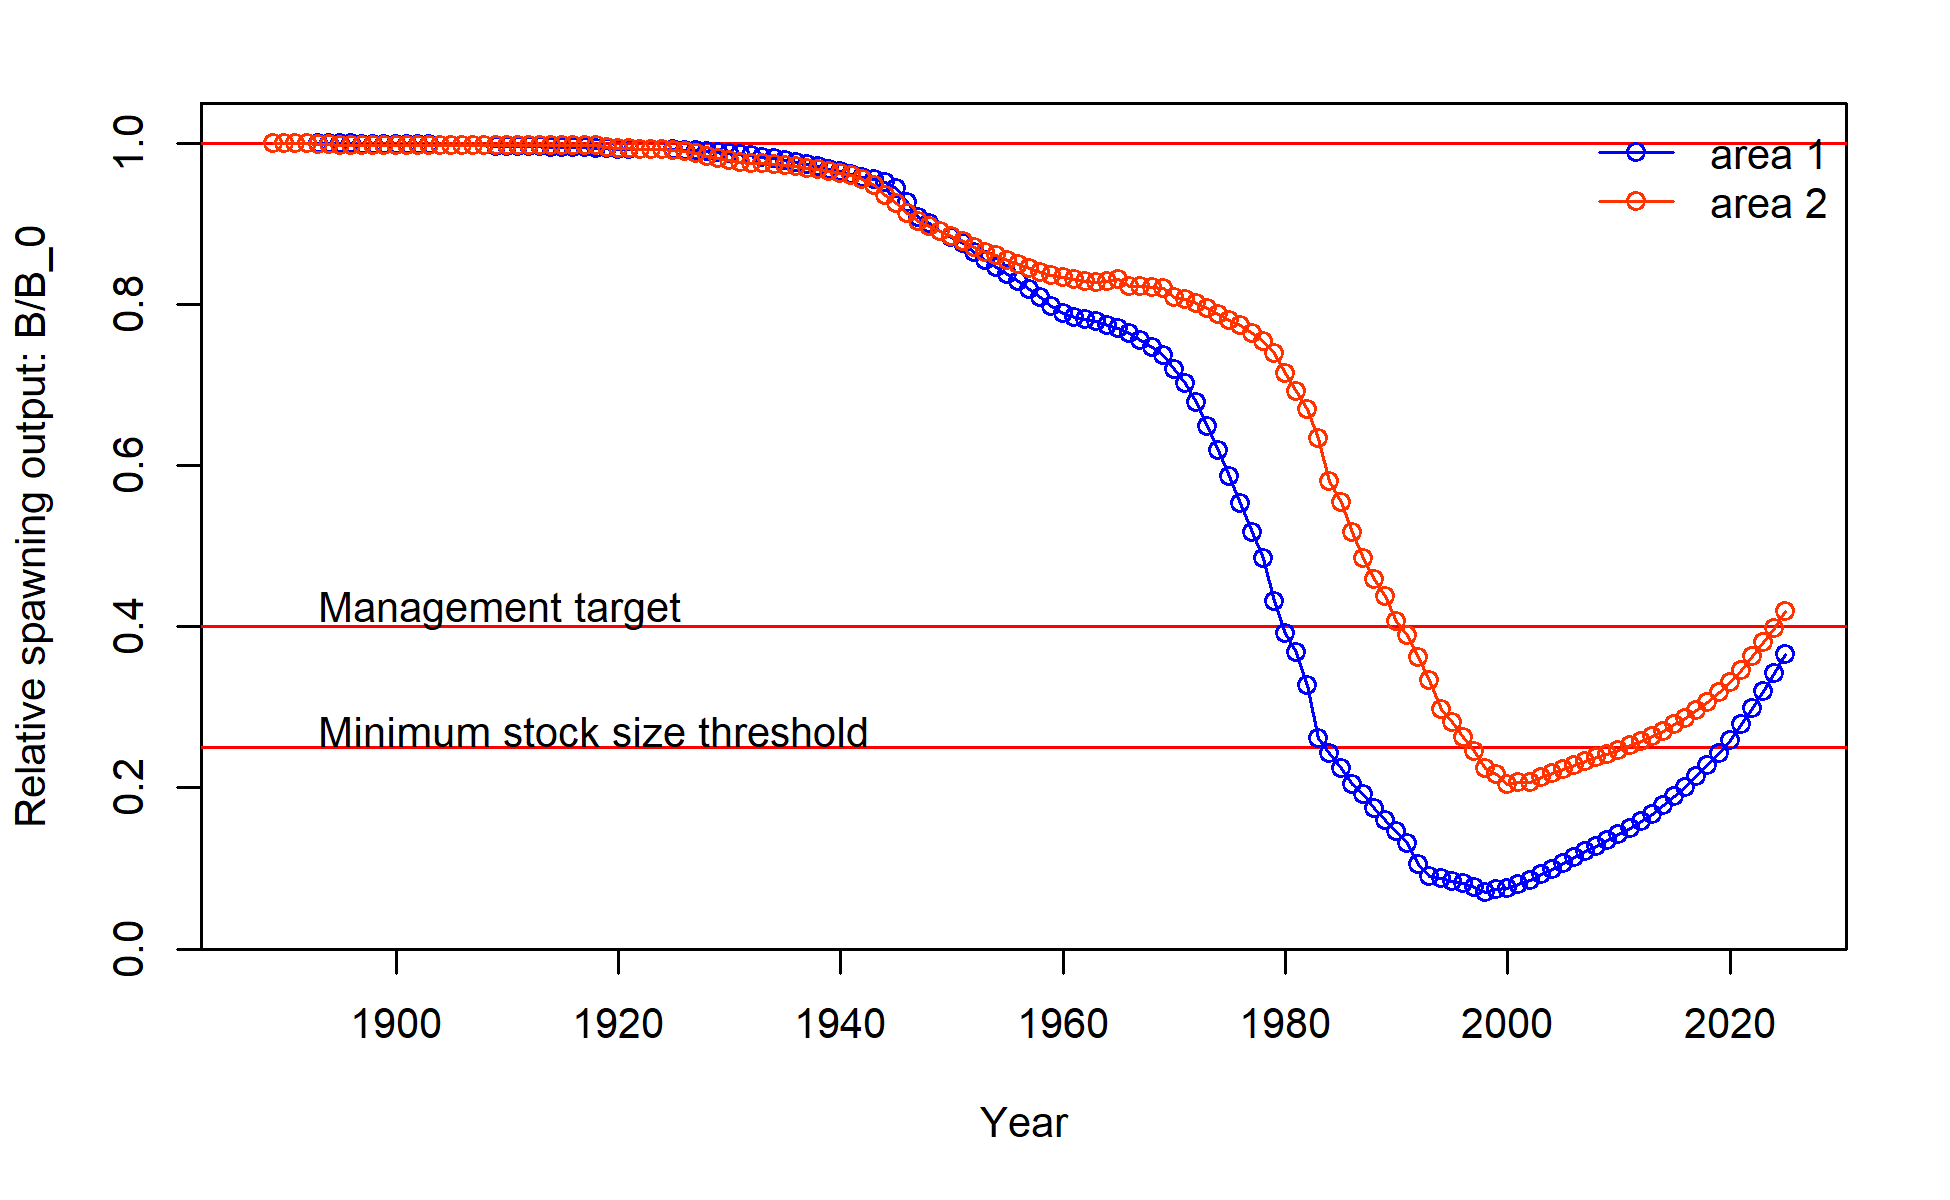
\includegraphics{figures/r4ss_plots/plots/ts10_Relative_spawning_output.png}

}

\caption{\label{fig-status-area-es}Time series of relative spawning
output estimated by area (area 1= California, area 2 = Oregon and
Washington).}

\end{figure}%

\clearpage

\subsection*{Recruitment}\label{recruitment}
\addcontentsline{toc}{subsection}{Recruitment}

The largest estimated recruitment events were in 1971, followed by more
recently, in 2013 and 2008 (Figure~\ref{fig-es-recruits},
Figure~\ref{fig-es-recdev}, Table~\ref{tbl-es-recr}). Trends in
recruitment are largely consistent with the previous assessment, apart
from the most recent elevated time period that is more informed with
additional length and age composition data. Recruits for this assessment
appear to have extended this more recent time period starting in 2005,
with peaks in 2008 and 2013, and and lower recruitment in 2017.

\begingroup
\fontsize{9.0pt}{10.8pt}\selectfont

\begin{longtable}{>{\centering\arraybackslash}p{\dimexpr 56.25pt -2\tabcolsep-1.5\arrayrulewidth}>{\centering\arraybackslash}p{\dimexpr 56.25pt -2\tabcolsep-1.5\arrayrulewidth}>{\centering\arraybackslash}p{\dimexpr 56.25pt -2\tabcolsep-1.5\arrayrulewidth}>{\centering\arraybackslash}p{\dimexpr 56.25pt -2\tabcolsep-1.5\arrayrulewidth}>{\centering\arraybackslash}p{\dimexpr 56.25pt -2\tabcolsep-1.5\arrayrulewidth}>{\centering\arraybackslash}p{\dimexpr 56.25pt -2\tabcolsep-1.5\arrayrulewidth}>{\centering\arraybackslash}p{\dimexpr 56.25pt -2\tabcolsep-1.5\arrayrulewidth}}

\caption{\label{tbl-es-recr}Estimated recent trend in recruitment
(1,000s) and recruitment deviations and the 95 percent confidence
intervals.}

\tabularnewline

\toprule
Year & Recruitment (1,000s) & Lower Interval (1,000s) & Upper Interval (1,000s) & Recruitment Deviations & Lower Interval & Upper Interval \\ 
\midrule\addlinespace[2.5pt]
2015 & 359 & 200 & 643 & 0.729 & 0.153 & 1.306 \\ 
2016 & 242 & 126 & 467 & 0.315 & -0.347 & 0.977 \\ 
2017 & 121 & 56 & 259 & -0.404 & -1.193 & 0.386 \\ 
2018 & 115 & 53 & 250 & -0.472 & -1.276 & 0.331 \\ 
2019 & 118 & 54 & 262 & -0.467 & -1.291 & 0.357 \\ 
2020 & 117 & 51 & 267 & -0.501 & -1.364 & 0.362 \\ 
2021 & 153 & 64 & 364 & -0.259 & -1.172 & 0.655 \\ 
2022 & 174 & 70 & 429 & -0.154 & -1.107 & 0.800 \\ 
2023 & 179 & 72 & 445 & -0.141 & -1.102 & 0.819 \\ 
2024 & 209 & 82 & 531 & 0.000 & -0.980 & 0.980 \\ 
2025 & 211 & 83 & 537 & 0.000 & -0.980 & 0.980 \\ 
\bottomrule

\end{longtable}

\endgroup

\begin{figure}[H]

\centering{

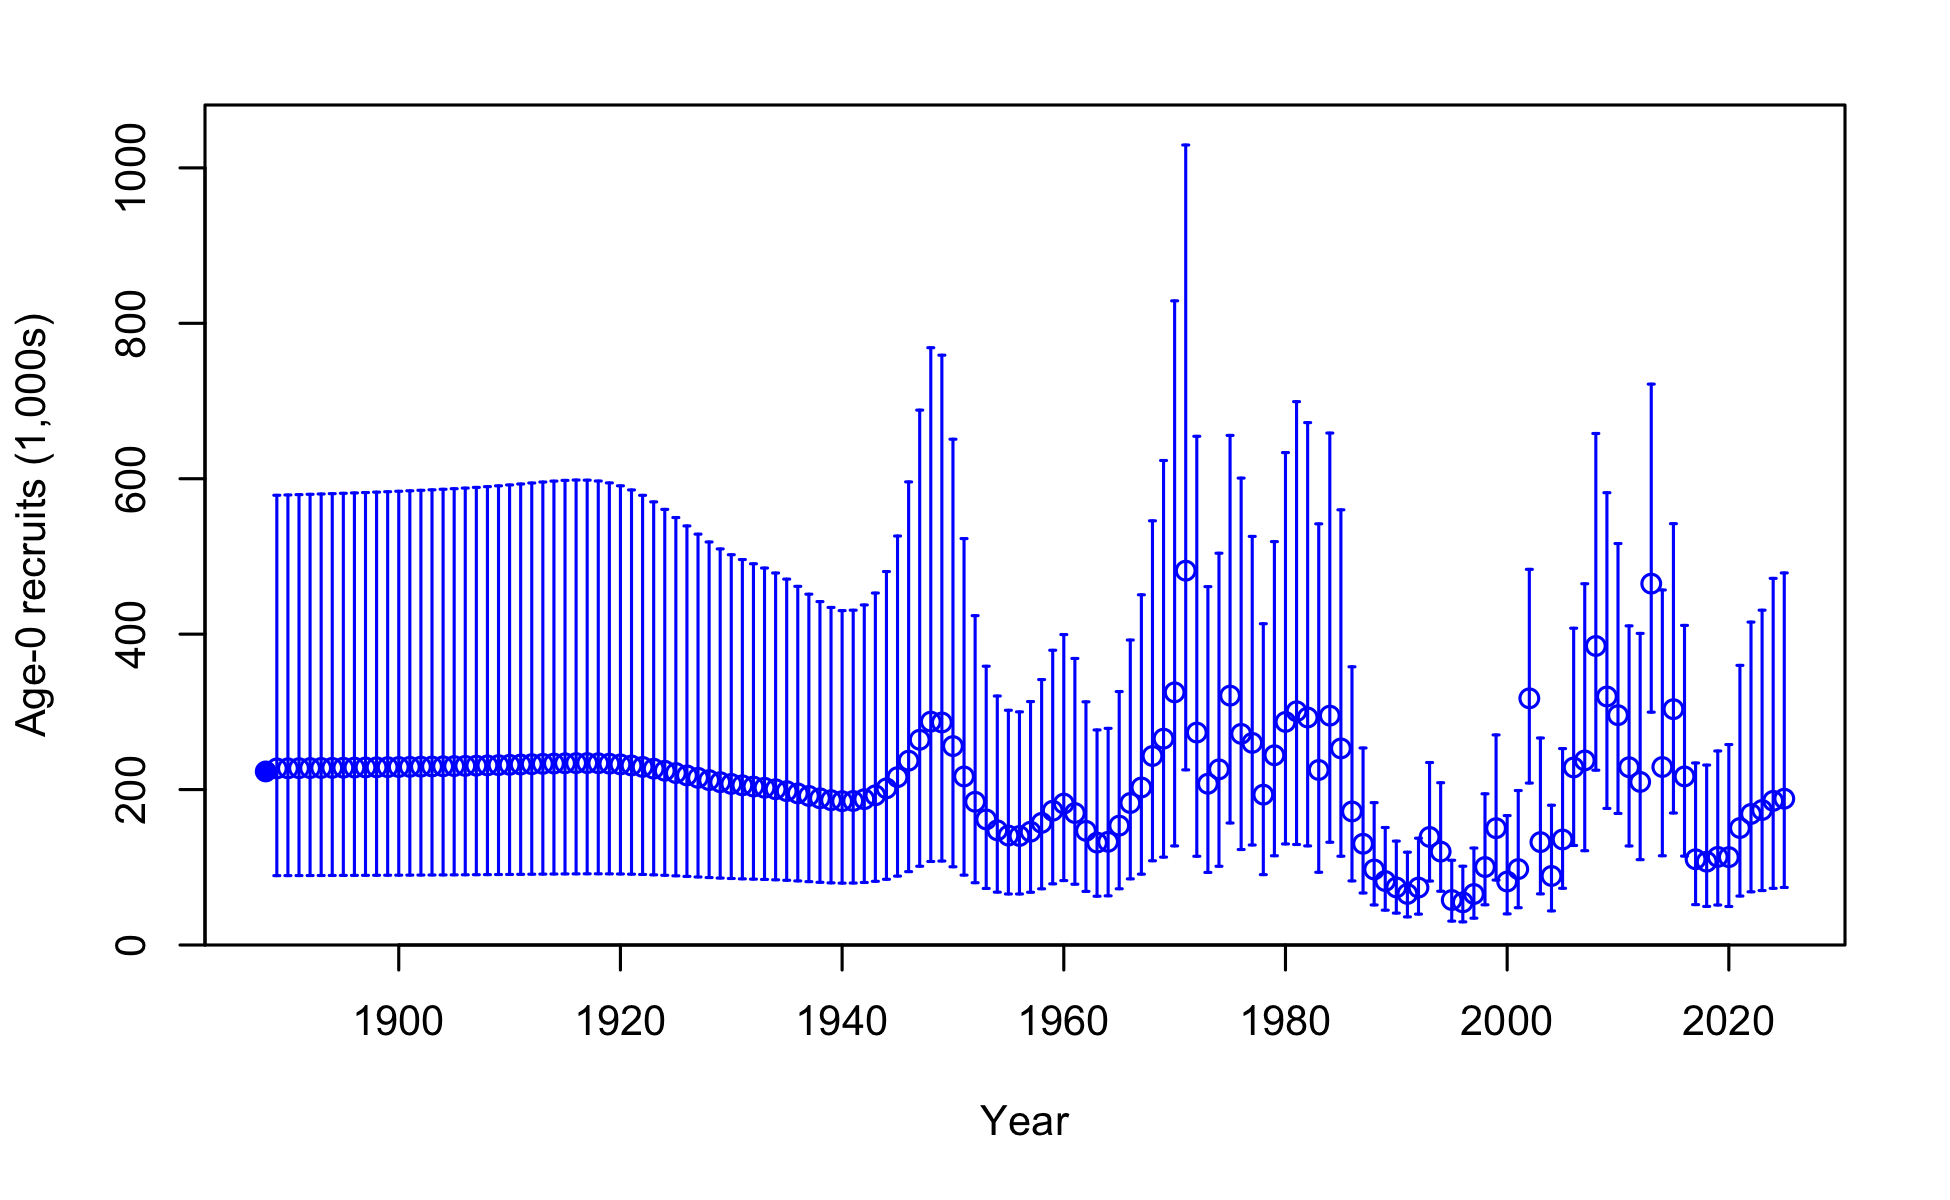
\includegraphics{figures/r4ss_plots/plots/ts11_Age-0_recruits_(1000s)_with_95_asymptotic_intervals.png}

}

\caption{\label{fig-es-recruits}Time series of estimated yelloweye
rockfish recruitments for the base model (circles) with approximate 95\%
intervals (vertical lines).}

\end{figure}%

\begin{figure}[H]

\centering{

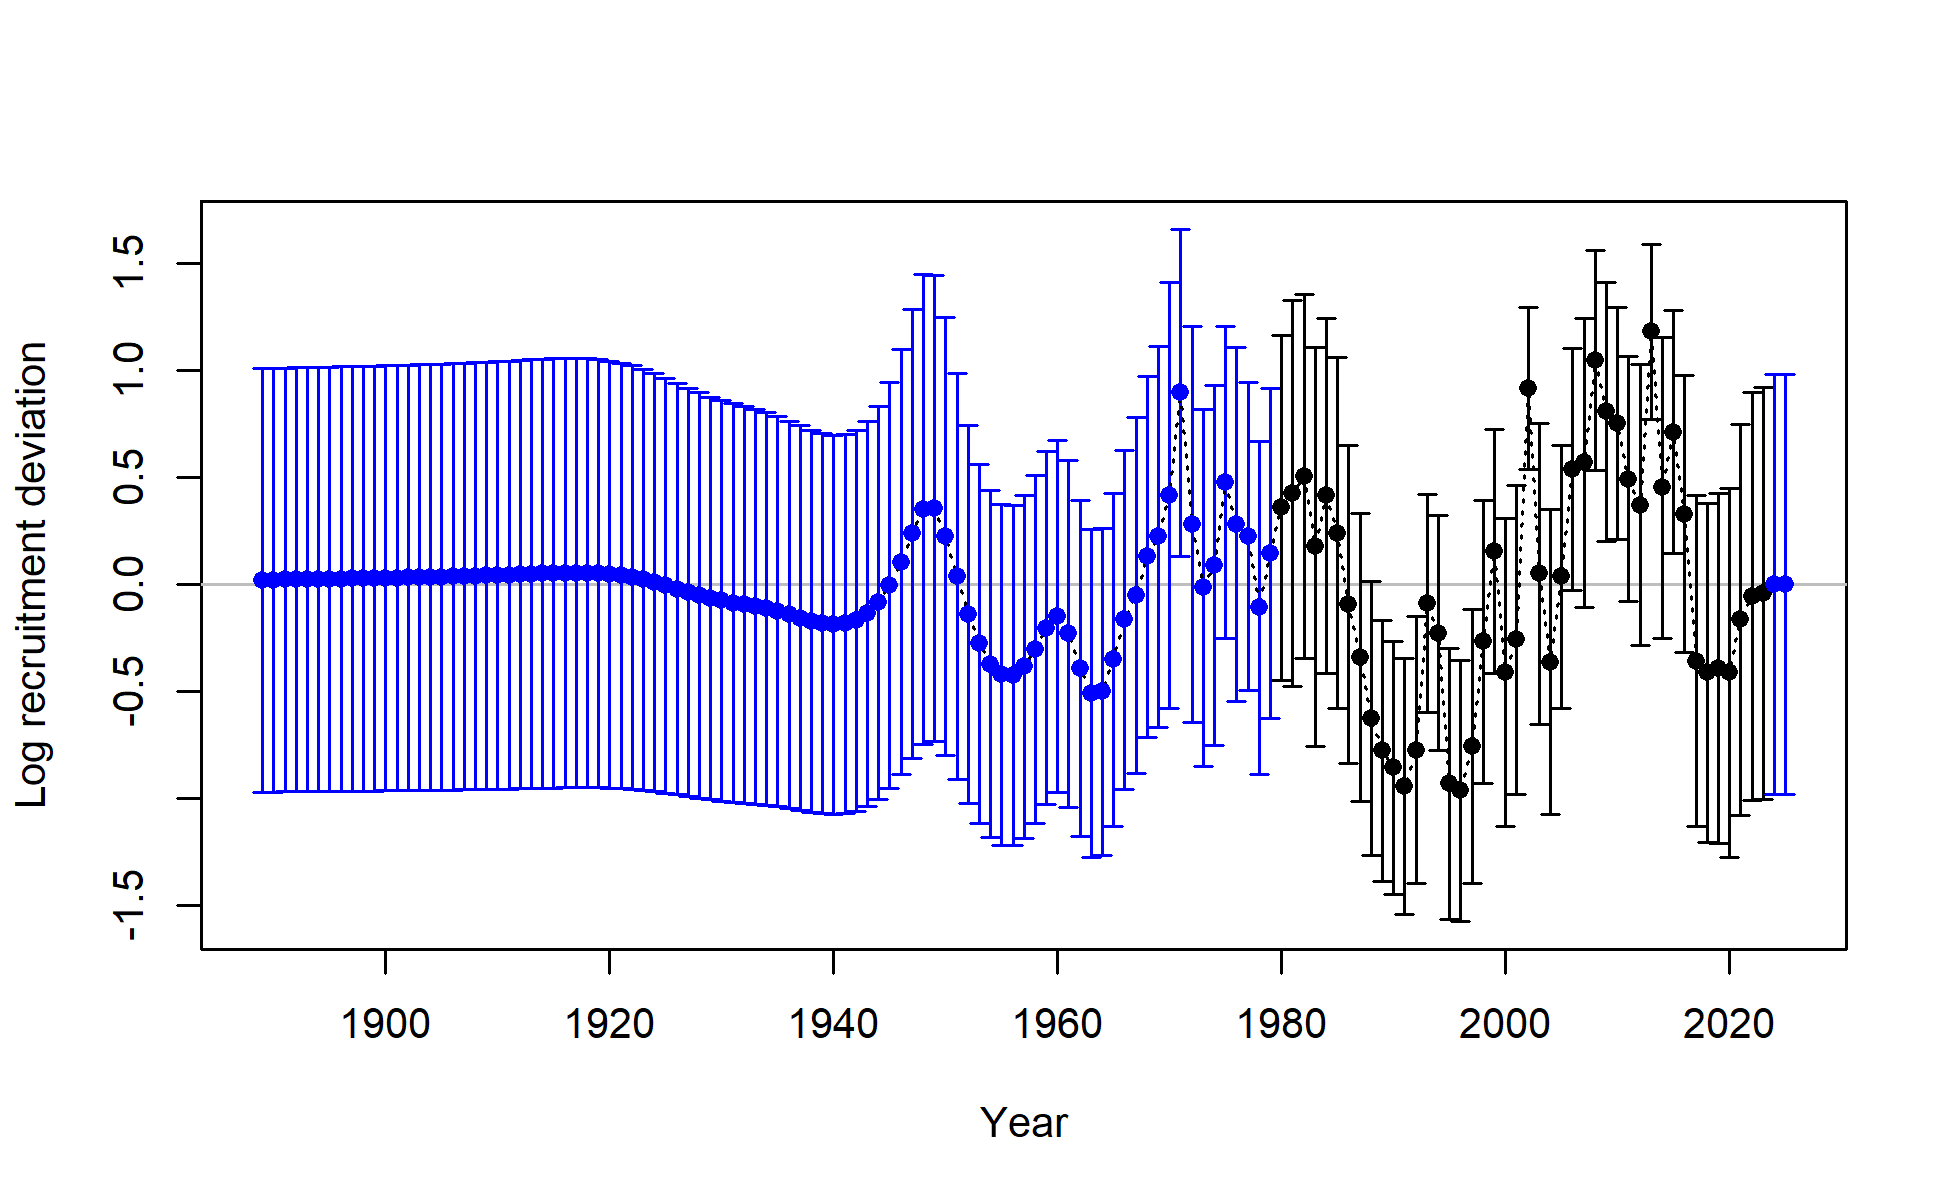
\includegraphics{figures/r4ss_plots/plots/recdevs2_withbars.png}

}

\caption{\label{fig-es-recdev}Estimated recruitment deviations with 95\%
intervals.}

\end{figure}%

\subsection*{Exploitation status}\label{exploitation-status}
\addcontentsline{toc}{subsection}{Exploitation status}

This assessment estimates that the stock of Yelloweye Rockfish off the
continental U.S. Pacific Coast is currently at 40.1\% of its unexploited
level. This is above the overfished threshold of SO25\%, and slightly
above the management target SO40\% of unfished spawning output. Fishing
intensity increased throughout the 1900s as the stock was fished down,
until stabilizing at peak intensity between the mid1980s and late 1990s
and substantially decreasing in the late 1990s and early 2000s. Fishing
intensity has since been relatively stable (Figure~\ref{fig-es-kobe},
Table~\ref{tbl-es-spr}).

\begin{figure}[H]

\centering{

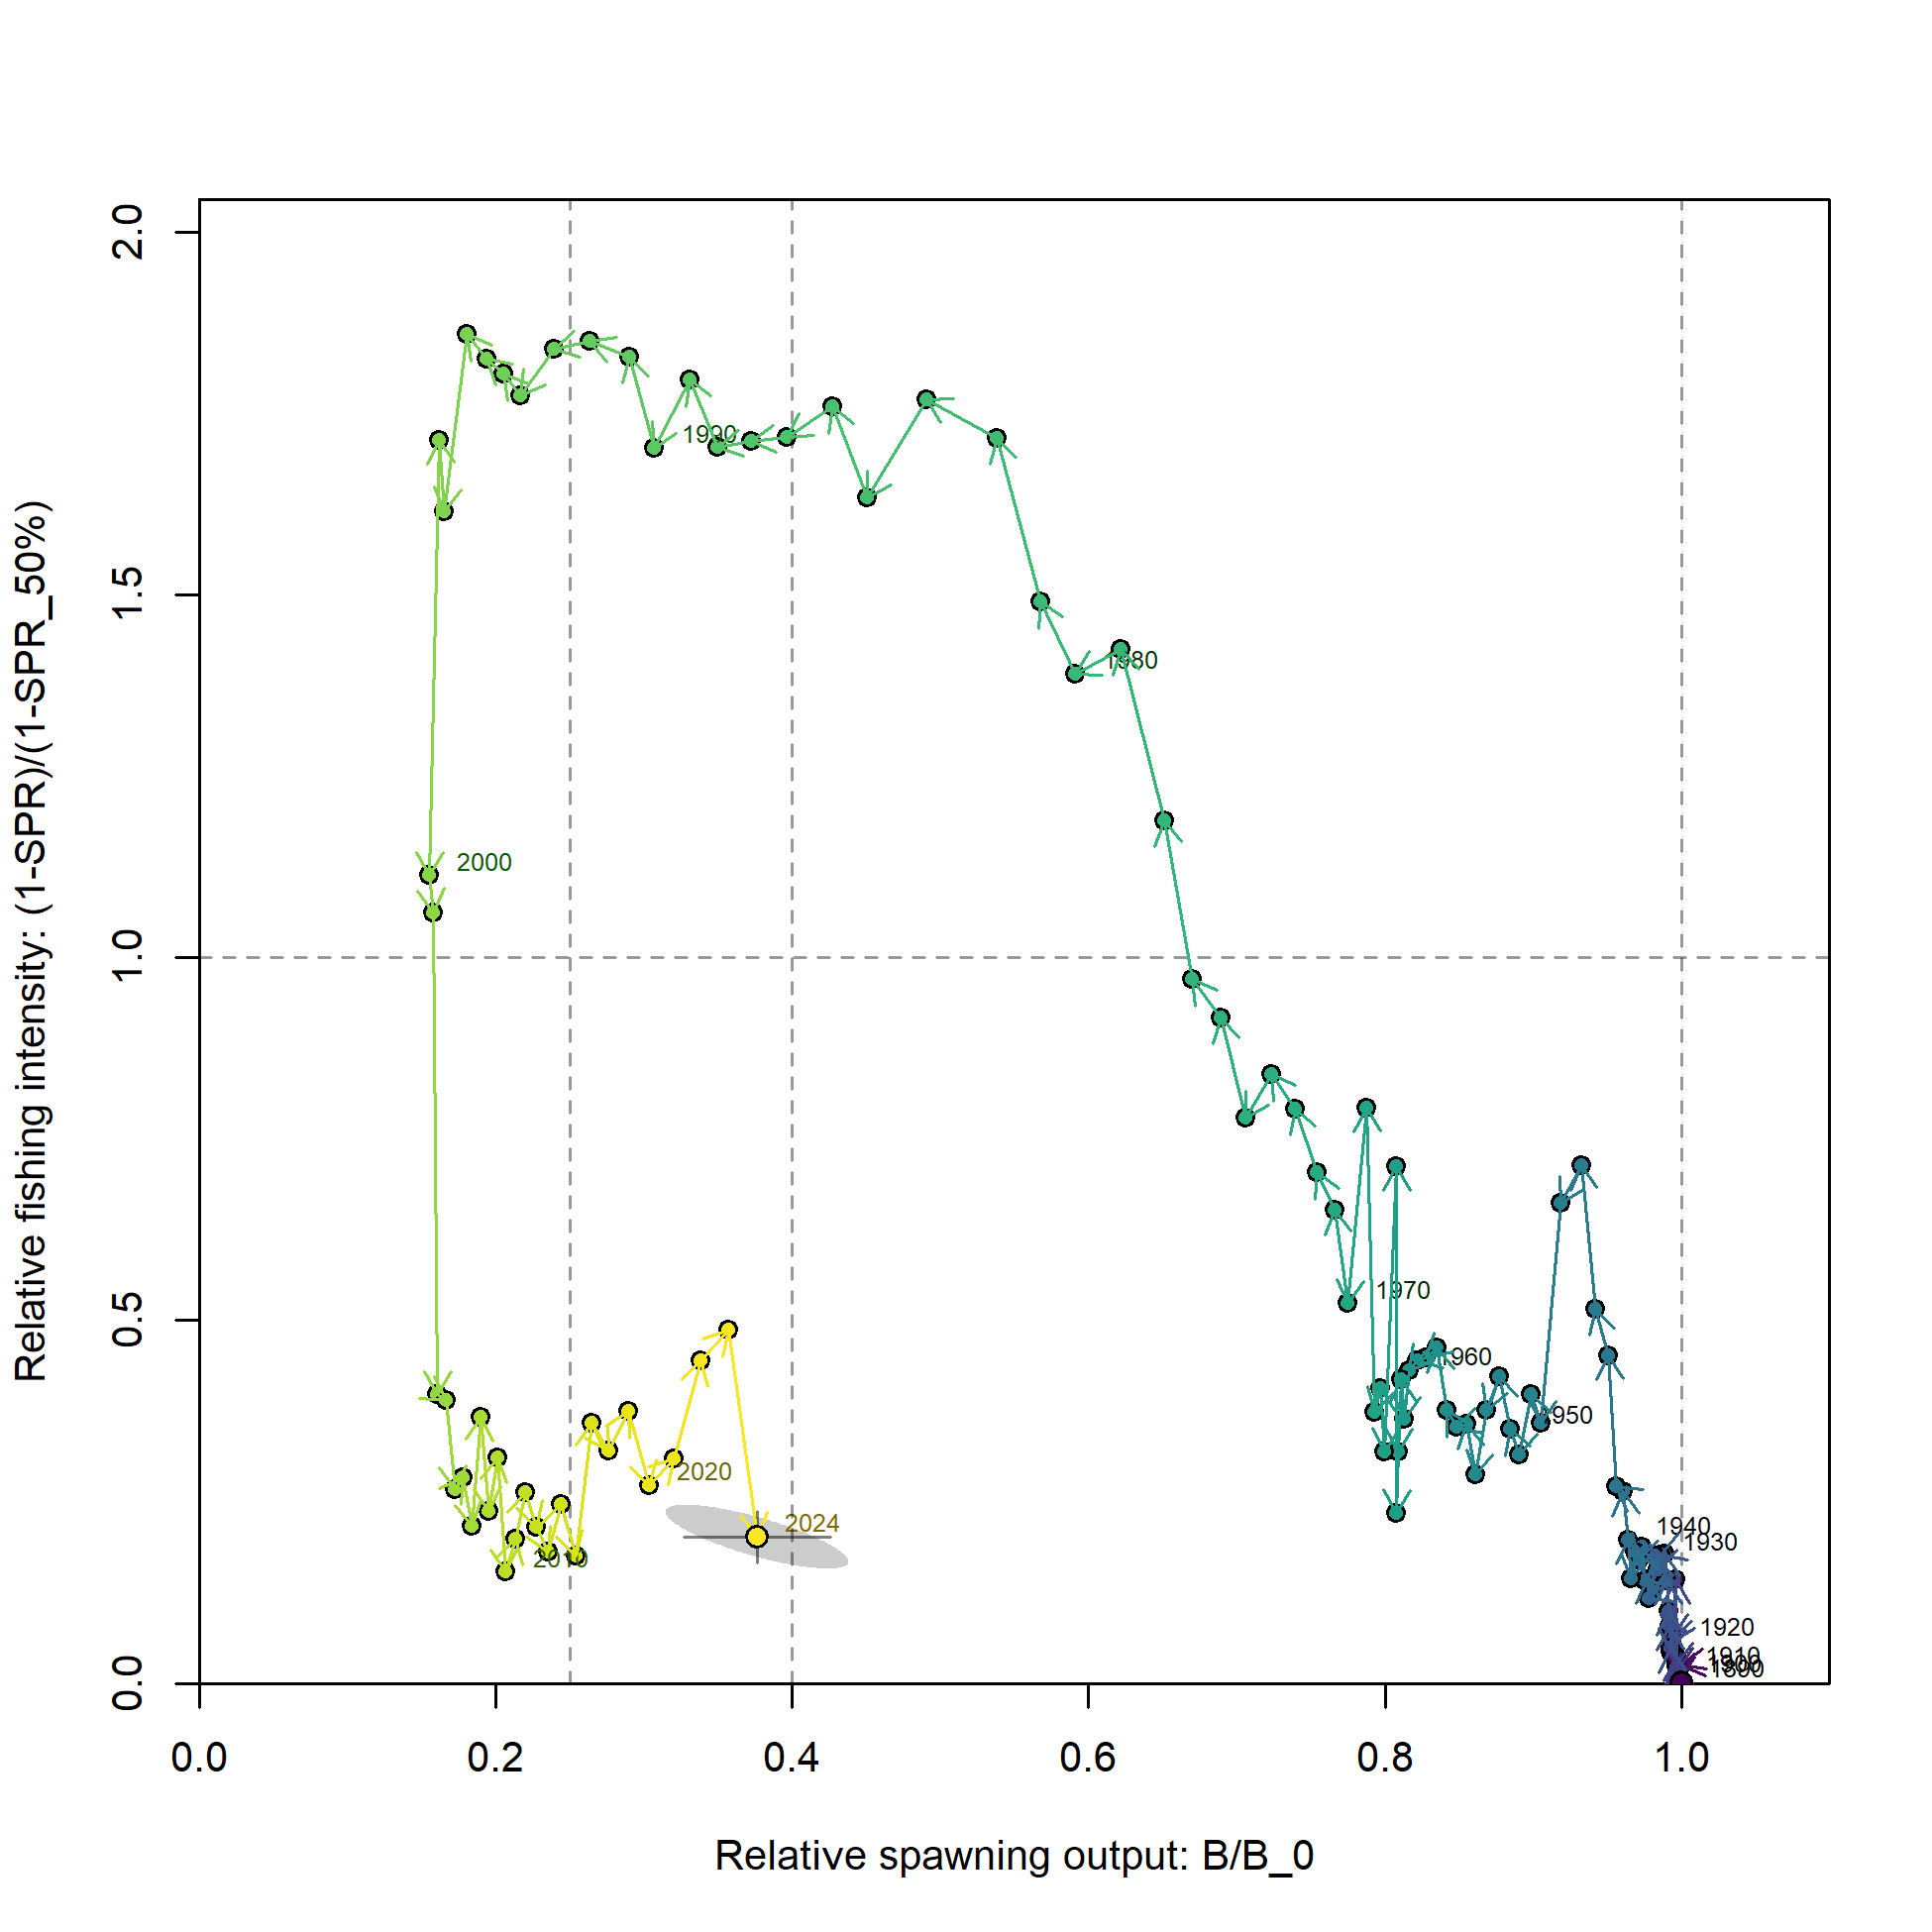
\includegraphics{figures/r4ss_plots/plots/SPR4_phase.png}

}

\caption{\label{fig-es-kobe}Phase plot of fishing intensity versus
fraction unfished. Each point represents the biomass ratio at the start
of the year and the relative fishing intensity in that same year. Lines
through the final point show 95\% intervals based on the asymptotic
uncertainty for each dimension. The shaded ellipse is a 95\% region
which accounts for the estimated correlation between the two
quantities.}

\end{figure}%

\clearpage

\begingroup
\fontsize{9.0pt}{10.8pt}\selectfont

\begin{longtable}{>{\centering\arraybackslash}p{\dimexpr 60.00pt -2\tabcolsep-1.5\arrayrulewidth}>{\centering\arraybackslash}p{\dimexpr 60.00pt -2\tabcolsep-1.5\arrayrulewidth}>{\centering\arraybackslash}p{\dimexpr 60.00pt -2\tabcolsep-1.5\arrayrulewidth}>{\centering\arraybackslash}p{\dimexpr 60.00pt -2\tabcolsep-1.5\arrayrulewidth}>{\centering\arraybackslash}p{\dimexpr 60.00pt -2\tabcolsep-1.5\arrayrulewidth}>{\centering\arraybackslash}p{\dimexpr 60.00pt -2\tabcolsep-1.5\arrayrulewidth}>{\centering\arraybackslash}p{\dimexpr 60.00pt -2\tabcolsep-1.5\arrayrulewidth}}

\caption{\label{tbl-es-spr}Estimated recent trend in relative fishing
intensity (1-SPR)/(1-SPR50\%), where SPR is the spawning potential
ratio, and the exploitation rate, along with the 95 percent confidence
intervals for both quantities.}

\tabularnewline

\toprule
Year & (1-SPR)/(1-SPR50\%) & Lower Interval (SPR) & Upper Interval (SPR) & Exploitation Rate & Lower Interval (Rate) & Upper Interval (Rate) \\ 
\midrule\addlinespace[2.5pt]
2015 & 0.244 & 0.201 & 0.286 & 0.004 & 0.003 & 0.005 \\ 
2016 & 0.174 & 0.143 & 0.204 & 0.003 & 0.002 & 0.003 \\ 
2017 & 0.355 & 0.296 & 0.414 & 0.006 & 0.005 & 0.007 \\ 
2018 & 0.317 & 0.264 & 0.370 & 0.005 & 0.004 & 0.006 \\ 
2019 & 0.371 & 0.310 & 0.431 & 0.006 & 0.005 & 0.007 \\ 
2020 & 0.270 & 0.225 & 0.314 & 0.004 & 0.004 & 0.005 \\ 
2021 & 0.306 & 0.255 & 0.358 & 0.005 & 0.004 & 0.006 \\ 
2022 & 0.441 & 0.372 & 0.509 & 0.007 & 0.006 & 0.009 \\ 
2023 & 0.482 & 0.408 & 0.555 & 0.008 & 0.007 & 0.010 \\ 
2024 & 0.357 & 0.299 & 0.414 & 0.006 & 0.005 & 0.007 \\ 
\bottomrule

\end{longtable}

\endgroup

\subsection*{Ecosystem considerations}\label{ecosystem-considerations}
\addcontentsline{toc}{subsection}{Ecosystem considerations}

No ecosystem or environmental data was used in the previous Yelloweye
Rockfish assessment and no new data were considered for this update
assessment.

\subsection*{Reference points}\label{reference-points}
\addcontentsline{toc}{subsection}{Reference points}

A list of estimates of the current state of the population, as well as
reference points based on 1) a target unfished spawning output of 40\%,
2) a spawning potential ratio of 0.5, and 3) the model estimate of
maximum sustainable yield, are all listed in
Table~\ref{tbl-ref-points-es-1}. Unfished spawning stock output for
Yelloweye Rockfish was estimated to be 1190 million eggs (95\%
confidence interval: 1,048.1 - 1,331.9 million eggs). The management
target for Yelloweye Rockfish is defined as 40\% of the unfished
spawning output (SO40\%), which is estimated by the model to be 476
million eggs (95\% confidence interval: 419 - 533), which corresponds to
an exploitation rate of 0.026. This harvest rate provides an equilibrium
yield of 122 mt at SO40\% (95\% confidence interval: 108 - 137 mt).

\clearpage

\begingroup
\fontsize{9.0pt}{10.8pt}\selectfont

\begin{longtable}{lrrr}

\caption{\label{tbl-ref-points-es-1}Summary of reference points and
management quantities, including estimates of the 95 percent confidence
intervals. SO is spawning output, SPR is the spawning potential ratio,
and MSY is maximum sustainable yield.}

\tabularnewline

\toprule
Reference Point & Estimate & Lower Interval & Upper Interval \\ 
\midrule\addlinespace[2.5pt]
Unfished Spawning output & 1,190.0 & 1,048.1 & 1,331.9 \\ 
Unfished Age 8+ Biomass (mt) & 10,331 & 9,101 & 11,561 \\ 
Unfished Recruitment (R0) & 242 & 213 & 271 \\ 
2025 Spawning output & 478 & 384 & 571 \\ 
2025 Fraction Unfished & 0.401 & 0.349 & 0.453 \\ 
Reference Points Based SO40\% & — & — & — \\ 
Proxy Spawning output SO40\% & 476 & 419 & 533 \\ 
SPR Resulting in SO40\% & 0.458 & 0.458 & 0.458 \\ 
Exploitation Rate Resulting in SO40\% & 0.026 & 0.026 & 0.027 \\ 
Yield with SPR Based On SO40\% (mt) & 122 & 108 & 137 \\ 
Reference Points Based on SPR Proxy for MSY & — & — & — \\ 
Proxy Spawning output (SPR50) & 531 & 468 & 594 \\ 
SPR50 & 0.500 & — & — \\ 
Exploitation Rate Corresponding to SPR50 & 0.023 & 0.023 & 0.023 \\ 
Yield with SPR50 at SO SPR (mt) & 117 & 103 & 131 \\ 
Reference Points Based on Estimated MSY Values & — & — & — \\ 
Spawning output at MSY (SO MSY) & 343 & 303 & 384 \\ 
SPR MSY & 0.358 & 0.356 & 0.359 \\ 
Exploitation Rate Corresponding to SPR MSY & 0.037 & 0.036 & 0.037 \\ 
MSY (mt) & 128 & 113 & 143 \\ 
\bottomrule

\end{longtable}

\endgroup

\clearpage

\subsection*{Management performance}\label{management-performance}
\addcontentsline{toc}{subsection}{Management performance}

Recent trends in total catch relative to management guidelines is
available in Table~\ref{tbl-es-management} and shows that total catch of
Yelloweye Rockfish has remained below both the \gls{ofl} and \gls{acl}
in each year since the previous assessment. Catch in
Table~\ref{tbl-es-management} combines the two areas in this model as
catch limits for Yelloweye Rockfish are managed as a single coast wide
unit and includes both landings and estimated discard mortality.

\begingroup
\fontsize{9.0pt}{10.8pt}\selectfont

\begin{longtable}{rrrrr}

\caption{\label{tbl-es-management}Recent trend in the overfishing limits
(OFL), the acceptable biological catches (ABCs), the annual catch limits
(ACLs), and the total dead catch (landings + discards) all in metric
tons (mt).}

\tabularnewline

\toprule
Year & OFL (mt) & ABC (mt) & ACL (mt) & Catch (mt) \\ 
\midrule\addlinespace[2.5pt]
2015 & 52 & 43 & 18 & 12 \\ 
2016 & 52 & 43 & 19 & 9 \\ 
2017 & 57 & 47 & 20 & 20 \\ 
2018 & 58 & 48 & 20 & 19 \\ 
2019 & 82 & 74 & 48 & 23 \\ 
2020 & 84 & 77 & 49 & 18 \\ 
2021 & 97 & 83 & 50 & 21 \\ 
2022 & NA & NA & NA & 34 \\ 
2023 & 90 & 75 & 52 & 39 \\ 
2024 & 91 & 76 & 53 & 29 \\ 
\bottomrule

\end{longtable}

\endgroup

\subsection*{Harvest projections}\label{harvest-projections}
\addcontentsline{toc}{subsection}{Harvest projections}

This section will be updated after SSC GFSC review.

\clearpage

\begingroup
\fontsize{9.0pt}{10.8pt}\selectfont

\begin{longtable}{>{\centering\arraybackslash}p{\dimexpr 56.25pt -2\tabcolsep-1.5\arrayrulewidth}>{\centering\arraybackslash}p{\dimexpr 56.25pt -2\tabcolsep-1.5\arrayrulewidth}>{\centering\arraybackslash}p{\dimexpr 56.25pt -2\tabcolsep-1.5\arrayrulewidth}>{\centering\arraybackslash}p{\dimexpr 56.25pt -2\tabcolsep-1.5\arrayrulewidth}>{\centering\arraybackslash}p{\dimexpr 56.25pt -2\tabcolsep-1.5\arrayrulewidth}>{\centering\arraybackslash}p{\dimexpr 56.25pt -2\tabcolsep-1.5\arrayrulewidth}>{\centering\arraybackslash}p{\dimexpr 56.25pt -2\tabcolsep-1.5\arrayrulewidth}>{\centering\arraybackslash}p{\dimexpr 56.25pt -2\tabcolsep-1.5\arrayrulewidth}>{\centering\arraybackslash}p{\dimexpr 56.25pt -2\tabcolsep-1.5\arrayrulewidth}>{\centering\arraybackslash}p{\dimexpr 56.25pt -2\tabcolsep-1.5\arrayrulewidth}}

\caption{\label{tbl-es-projections}Potential OFLs (mt), ABCs (mt), ACLs
(mt), the buffer between the OFL and ABC, estimated spawning output, and
fraction of unfished spawning output with adopted OFLs and ACLs and
assumed catch for the first two years of the projection period.}

\tabularnewline

\toprule
Year & Adopted OFL (mt) & Adopted ACL (mt) & Assumed Catch (mt) & OFL (mt) & Buffer & ABC (mt) & ACL (mt) & Spawning output & Fraction Unfished \\ 
\midrule\addlinespace[2.5pt]
2025 & 105.8 & 55.8 & 45.7 & — & — & — & — & 477.630 & 0.401 \\ 
2026 & 108.3 & 56.6 & 46.4 & — & — & — & — & 502.268 & 0.422 \\ 
2027 & — & — & — & 129.3 & 0.873 & 112.9 & 112.9 & 526.772 & 0.443 \\ 
2028 & — & — & — & 130.9 & 0.864 & 113.1 & 113.1 & 543.555 & 0.457 \\ 
2029 & — & — & — & 132.0 & 0.856 & 113.0 & 113.0 & 558.406 & 0.469 \\ 
2030 & — & — & — & 132.7 & 0.848 & 112.6 & 112.6 & 570.839 & 0.480 \\ 
2031 & — & — & — & 133.1 & 0.840 & 111.8 & 111.8 & 580.654 & 0.488 \\ 
2032 & — & — & — & 133.3 & 0.832 & 110.9 & 110.9 & 587.932 & 0.494 \\ 
2033 & — & — & — & 133.2 & 0.824 & 109.8 & 109.8 & 592.973 & 0.498 \\ 
2034 & — & — & — & 133.1 & 0.817 & 108.8 & 108.8 & 596.202 & 0.501 \\ 
2035 & — & — & — & 132.9 & 0.809 & 107.6 & 107.6 & 598.069 & 0.503 \\ 
2036 & — & — & — & 132.8 & 0.801 & 106.3 & 106.3 & 599.025 & 0.503 \\ 
\bottomrule

\end{longtable}

\endgroup

\clearpage

\subsection*{Decision table}\label{decision-table}
\addcontentsline{toc}{subsection}{Decision table}

This section will be updated after SSC GFSC review.

\begin{table}[H]

\caption{\label{tbl-es-decision-1}Decision table with 12-year
projections. `Mgmt' refers to the management scenario (A) with the
default harvest control rule \(P^* = 0.40\). In each case the 2025 and
2026 catches are fixed at the estimates provided by the GMT. The catch
for the Washington recreational fleet is input in numbers so the GMT
estimate was converted from 3.22 metric tons to 1.53 thousands of fish
based on a mean weight of 2.105 kg estimated by SS3 for this fleet in
2024. The alternative states of nature (`Low', `Base', and `High' as
discussed in the text) are provided in the columns, with Spawning Output
(`Spawn', in millions of eggs) and Fraction of unfished spawning output
(`Frac') provided for each state.}

\centering{

\centering\centering
\fontsize{9}{11}\selectfont
\begin{tabular}[t]{>{}llr>{\raggedleft\arraybackslash}p{3.5em}>{\raggedleft\arraybackslash}p{3.5em}>{\raggedleft\arraybackslash}p{3.5em}>{\raggedleft\arraybackslash}p{3.5em}>{\raggedleft\arraybackslash}p{3.5em}>{\raggedleft\arraybackslash}p{3.5em}}
\toprule
Mgmt & Year & Catch & Low Spawn & Low Frac & Base Spawn & Base Frac & High Spawn & High Frac\\
\midrule
\textbf{A} & 2025 & 46 & 330.67 & 0.289 & 477.63 & 0.401 & 839.65 & 0.603\\
\textbf{} & 2026 & 46 & 347.96 & 0.305 & 502.27 & 0.422 & 878.58 & 0.630\\
\textbf{} & 2027 & 113 & 365.20 & 0.320 & 526.77 & 0.443 & 916.84 & 0.658\\
\textbf{} & 2028 & 113 & 374.94 & 0.328 & 543.56 & 0.457 & 946.40 & 0.679\\
\textbf{} & 2029 & 113 & 383.27 & 0.335 & 558.41 & 0.469 & 972.47 & 0.698\\
\textbf{} & 2030 & 113 & 389.86 & 0.341 & 570.84 & 0.480 & 994.20 & 0.713\\
\textbf{} & 2031 & 112 & 394.60 & 0.345 & 580.65 & 0.488 & 1011.25 & 0.726\\
\textbf{} & 2032 & 111 & 397.56 & 0.348 & 587.93 & 0.494 & 1023.78 & 0.735\\
\textbf{} & 2033 & 110 & 398.98 & 0.349 & 592.97 & 0.498 & 1032.35 & 0.741\\
\textbf{} & 2034 & 109 & 399.19 & 0.349 & 596.20 & 0.501 & 1037.71 & 0.745\\
\textbf{} & 2035 & 108 & 398.51 & 0.349 & 598.07 & 0.503 & 1040.63 & 0.747\\
\textbf{} & 2036 & 106 & 397.30 & 0.348 & 599.03 & 0.503 & 1041.85 & 0.748\\
\bottomrule
\end{tabular}

}

\end{table}%

\subsection*{Scientific uncertainty}\label{scientific-uncertainty}
\addcontentsline{toc}{subsection}{Scientific uncertainty}

The model estimate of the log-scale standard deviation of the 2025
spawning output is 0.0996. The model estimate of the log-scale standard
deviation of the 2025 \gls{ofl} is 0.095. Each of these are likely
underestimates of overall uncertainty due to the necessity to fix
several key population dynamics parameters (e.g.~steepness and
recruitment variance) and also because there is no explicit
incorporation of model structural uncertainty (although see the decision
table for alternative states of nature).

\subsection*{Research and data needs}\label{research-and-data-needs}
\addcontentsline{toc}{subsection}{Research and data needs}

Please refer to the 2017 benchmark assessment for a detailed list of
research and data needs for Yelloweye Rockfish (Gertseva and Cope
(2017)). In addition to those, the following research and
recommendations could improve the ability of future stock assessments to
determine the status and productivity of the Yelloweye Rockfish
population:

\begin{itemize}
\tightlist
\item
  Continue refining the ORFS index analysis and ultimately use either
  the ORBS or ORFS index to describe the CPUE trends in the Oregon
  recreational fishery after 2000.
\item
  Expand the IPHC age composition bins to an older maximum age for the
  IPHC age composition data to spread out the distribution of length
  data in the oldest age bins for conditional age-at-length.
\item
  Explore potential indices of abundance in untrawlable areas.
\end{itemize}

\subsection*{Rebuilding projections}\label{rebuilding-projections}
\addcontentsline{toc}{subsection}{Rebuilding projections}

This section will be updated after SSC GFSC review.

\pagebreak

\newpage{}

\setlength{\parskip}{5mm plus1mm minus1mm}
\pagenumbering{arabic}
\setcounter{page}{1}
\setcounter{section}{0}
\renewcommand{\thefigure}{\arabic{figure}}
\renewcommand{\thetable}{\arabic{table}}
\setcounter{table}{0}
\setcounter{figure}{0}

\clearpage

\section{Introduction}\label{introduction}

Yelloweye Rockfish (\emph{Sebastes ruberrimus}) are found from the Gulf
of Alaska to northern Baja California in Mexico across the northeastern
Pacific Ocean (Hart 1973; Love, Yoklavich, and Thorsteinson 2002). Their
core distribution is from southeast Alaska to central California on the
west coast of the United States (Love, Yoklavich, and Thorsteinson
2002). Yelloweye Rockfish in Puget Sound are considered isolated from
the coastal waters population (I. J. Stewart, Wallace, and McGilliard
2009) and have been listed as threatened under the Endangered Species
Act since 2010 (Drake et al. 2010).

Yelloweye Rockfish are strongly associated with rocky bottom habitat,
particularly areas of high relief (Love, Yoklavich, and Thorsteinson
2002), and adults are considered to be solitary and sedentary after
settlement (Coombs 1979; DeMott 1983). However, new tagging studies
suggest that adult Yelloweye Rockfish exhibit larger scale movement
patterns more commonly than previously considered (Hannah and Rankin
2011; Rasmuson et al. 2025).

There has been little advancement on information pertaining to the stock
structure of Yelloweye Rockfish since the previous benchmark assessment.
As noted in Gertseva and Cope (2017), there is evidence of genetic
differences between Canadian waters (Strait of Georgia) and West coast
coastal populations of Yelloweye Rockfish, but no evidence of
differentiation across coastal populations (Siegle et al. 2013). Gao et
al. (2010) found that there was complete mixing of offspring from Oregon
and Washington waters using otolith isotope analyses, indicating a
single spawning stock in this portion of the Yelloweye Rockfish stock.
Given the general perception of the sedentary nature of Yelloweye
Rockfish adults and the moderate amount of mixing that occurs during the
pelagic larval stage, the previous Yelloweye Rockfish assessment modeled
the West coast population as a two-area assessment (California and a
combined Oregon-Washington area) with a common stock recruitment
relationship (Gertseva and Cope 2017). This update assessment maintains
this basic structure.

\subsection{Life History}\label{life-history}

This section is not required for an update assessment; please refer to
the most recent full assessment (Gertseva and Cope 2017) for additional
information.

\subsection{Ecosystem considerations}\label{ecosystem-considerations-1}

This section is not required for an update assessment; please refer to
the most recent full assessment (Gertseva and Cope 2017) for additional
information.

\subsection{Fishery description}\label{fishery-description}

This section is not required for an update assessment; please refer to
the most recent full assessment (Gertseva and Cope 2017) for additional
information.

\subsection{Management History}\label{management-history}

Since the 2017 assessment, catch restrictions for Yelloweye Rockfish
have continued, though as the stock recovers, the rebuilding plan has
allowed for small catch increases that slightly loosened the
constraining impact of this species.

This section is not required for an update assessment; please refer to
the most recent full assessment (Gertseva and Cope 2017) and
Section~\ref{sec-mgmt} for additional information.

\subsection{Management performance}\label{sec-mgmt}

Yelloweye Rockfish removals have been substantially reduced since its
designation as overfished in 2002 through a variety of management
measures that eliminated retention in recreational fisheries, limited
commercial retention, created broad spatial closures, and implemented
new gear restrictions that reduced trawling in rocky habitats. Many of
these restrictions remain in effect, though as Yelloweye Rockfish and
other groundfish stocks have begun to rebuild, some management measures
have been modified or removed in recent years. These include some
additional allocations to recreational fisheries that remain constrained
by Yelloweye Rockfish estimated discard mortality, the recent removal of
the Yelloweye \gls{rca} for the trawl sector off of California and
Oregon, and eliminating some gear restrictions in the RCAs for the
non-trawl sector.

Recent trends in total catch relative to management guidelines are
available in Table~\ref{tbl-ye-management} and show that total catch of
Yelloweye Rockfish has remained below both the \gls{ofl} and \gls{acl}
in each year since the previous assessment. Catch in
Table~\ref{tbl-ye-management} combines the two areas in this model as
catch limits for Yelloweye Rockfish are managed as a single coast wide
unit and includes both landings and estimated discard mortality. As in
the previous assessment, total catches for each fleet in this update
include both landings and estimated dead discard mortality.

\subsection{Fisheries off Canada and
Alaska}\label{fisheries-off-canada-and-alaska}

This section is not required for an update assessment; please refer to
the most recent full assessment (Gertseva and Cope 2017) for additional
information.

\newpage{}

\section{Data}\label{sec-data}

A summary of available data by type and fleet used in the Yelloweye
Rockfish assessment is available in Figure~\ref{fig-data}. Data that
have changed or been added since the previous 2017 assessment are
summarized below. No new data sources were considered in this update
assessment.

Removals:

\begin{itemize}
\tightlist
\item
  Post-2016 landings and discards were added for all three states for
  the commercial and recreational fleets.
\item
  A new Oregon historical recreational catch reconstruction was
  incorporated, which covered 1979 - 2000.
\item
  A new Washington historical recreational catch reconstruction was
  provided by \gls{wdfw} and included changes to data from 1990-2016.
\end{itemize}

Composition Data:

\begin{itemize}
\tightlist
\item
  Length and age composition data were added from 2017 - 2024 for all
  states for the commercial and recreational fleets.
\item
  Length and age composition data were also extended for the
  \gls{indexwc} and the \gls{iphc} Longline survey.
\item
  Some length and age composition data from the 2017 assessment had
  minor errors in how sample numbers were calculated, ageing error
  assignment, or doubled age samples and thus needed to be fixed. See
  Section~\ref{sec-fd_comps} below.
\end{itemize}

Indices of Abundance:

\begin{itemize}
\tightlist
\item
  Indices that were updated with more recent data and/or updated
  methodology include:

  \begin{itemize}
  \tightlist
  \item
    Oregon Onboard Observer (2001 - 2024)
  \item
    Oregon \gls{orbs} Dockside (release only) (2004-2024)
  \item
    \gls{indexwc} (2003 - 2024)
  \item
    \gls{iphc} Longline Survey (2002 - 2024)
  \end{itemize}
\end{itemize}

Biological Data:

\begin{itemize}
\tightlist
\item
  Length-weight relationship parameters were updated to include all the
  recent (2017 - 2024) fishery-independent data.
\item
  Ageing error matrices were unchanged but some Oregon recreation ages
  were assigned the wrong ageing error in the 2017 assessment and were
  corrected based on ODFW recommendations.
\end{itemize}

\subsection{Fishery-Dependent Data}\label{fishery-dependent-data}

Updated fishery-dependent data, including removals, length and age
compositions, and indices of abundance are detailed below.

\subsubsection{Landings}\label{landings}

A summary of total removals are provided in Table~\ref{tbl-all_removals}
and Figure~\ref{fig-catch}.

Recent commercial landings (2017-2024) were obtained from
\href{www.pacfin.psmfc.org}{\gls{pacfin}} for California, Oregon and
Washington. For the period from 2016 through 2023, updated \gls{wcgop}
discard estimates were added to \gls{pacfin} landings by adding the
annual dead discard mortality rate for the commercial sector in the
\gls{gemm} recorded discards to obtain the total catch of Yelloweye
Rockfish within commercial fleets. At this time no \gls{wcgop} data were
available for 2024, so we used the average total discard for 2021-2023
to approximate total 2024 discards for each commercial fleet.

Bycatch for the At-Sea Pacific Hake fleet (A-SHOP) was updated from 2017
through 2024.

Recreational removals from \href{www.recfin.org}{\gls{recfin}} were
updated for California, Oregon and Washington from 2017 - 2024.
\gls{recfin} removals include an estimate of discard mortality and
represent total estimated removals. The (\gls{odfw}) provided updated
historical recreational removals for Oregon from 1979 through 2000
(Whitman 2024). The Washington Department of Fish and Wildlife
(\gls{wdfw}) provided updated historical recreational removals
(1967-1989) and \gls{osp} estimates (1990-2001). The historical
recreational removals for 1971, 1974, and 1979 were not available and
were filled in as the average of the two preceding and two following
years. Historical data were filtered to marine catch areas 1-4. For
\gls{osp} catch estimates, data included marine catch areas 1-4, up to
the Bonilla-Tatoosh line. \gls{wdfw} also provided updated catch
estimates for 2002-2004, which did not include discard mortality. To
adjust for this, we multiplied the average discard mortality rate from
the following five years (2005-2009) by the total discards to calculate
total mortality for those years.

\subsubsection{Fishery-Dependent Length and Age
Compositions}\label{sec-fd_comps}

Updated length composition data for commercial catches (trawl and
non-trawl) were available from \gls{pacfin} (extracted April 4, 2025)
and from \gls{wcgop} for all three states. These include the years 2017
- 2024 for \gls{pacfin} data and 2017 - 2023 for \gls{wcgop} data.
Updated recreational length composition data were available from
\gls{recfin} (extracted April 4, 2025) for all three states, and include
years 2017 - 2024. Additionally, updated length compositions from the
California On-Board CPFV Observer Sampling Program and from the Ocean
Recreational Fishery Survey (ORFS, previously the Oregon onboard
recreational observer program), both of which measure fish discarded at
sea, were also available up through 2024 on \gls{recfin}.

New commercial age composition data from \gls{pacfin} and \gls{wcgop}
for 2017-2024 was included for Oregon and Washington. No new commercial
age data were available from California. New recreational age
composition data was available from \gls{recfin} from 2017 - 2024 for
Washington only (extracted May 13, 2025). These data were collected in
the \gls{osp}. There were also some historical updates to Oregon and
Washington recreational age data provided by the state representatives.

In addition to extending the length data time series, we also fixed
minor data errors found in the 2017 assessment. For length composition
data, years with small samples sizes (N = 1) were excluded. There were
no changes in how commercial length sample numbers were calculated.
However, for all recent recreational fleet length data, the total number
of trips information used to calculate the number of samples was not
available. Using data from the 2017 assessment, we built fleet-specific
linear regressions to approximate the relationship of samples to the
number of fish. Then, we applied that regression to the total number of
fish for data between 2017 and 2024 to estimate the number of samples. A
future benchmark assessment should investigate how to get the number of
sampled trips from \gls{recfin} to calculate the number of samples using
the Stewart and Hamel (2014) method.

We also found that \gls{caal} data from the 2017 assessment had all
sample sizes and relative proportions doubled, potentially from when
Yelloweye Rockfish was changed from a two-sex to single-sex model. For
most fleets this was not a problem because the proportions of
age-at-length counts were the same, however, some of the commercial
fleets included discard age proportions that were not doubled, leading
to small differences in proportions. To fix the \gls{caal} data so it
accurately represented the number of fish in each age class, we either
rebuilt the entire fleet's \gls{caal} data frame using the most recently
pulled information from \gls{pacfin} and \gls{recfin}, or divided the
number of samples or relative proportions in each length bin by two. How
these problems were treated for each fleet specifically is detailed
below, including other minor data changes. Otherwise, length and age
composition data are unchanged from the previous assessment; please
refer to the most recent benchmark assessment (Gertseva and Cope 2017)
for additional information.

\paragraph{Fleet Specific Changes in the Compositional
Data}\label{fleet-specific-changes-in-the-compositional-data}

\begin{itemize}
\tightlist
\item
  Fleet 2. California Non-Trawl:

  \begin{itemize}
  \tightlist
  \item
    For ages, all the \gls{caal} and marginal ages (used to explore fits
    only, not included in the likelihood) data were recalculated using
    the most recent age data pulled from \gls{pacfin} and \gls{wcgop},
    to account for age doubling in 2017.
  \end{itemize}
\end{itemize}

Fleet 3. California Recreational:

\begin{itemize}
\tightlist
\item
  \gls{caal} data for 1979-1984 were doubled, so the number of samples
  and age-at-length proportions were divided by two.
\item
  \gls{caal} data for 2009-2016 were doubled, but the raw data we
  received from \gls{recfin} were correct, without doubled ages, so this
  time series was replaced with newly pulled data.
\item
  We then re-built the marginal age data from the updated \gls{caal} for
  both time periods because there were errors in previous data entry and
  sample number calculations.
\end{itemize}

Fleet 4. Oregon/Washington Trawl \& Fleet 5. Oregon/Washington
Non-Trawl:

\begin{itemize}
\tightlist
\item
  Both the OR/WA commercial fleets had all \gls{caal} and marginal age
  (not included in the likelihood) data recalculated using the most
  recent age data pulled from \gls{pacfin} and \gls{wcgop}, to account
  for age doubling in 2017.
\end{itemize}

Fleet 6. Oregon Recreational:

\begin{itemize}
\tightlist
\item
  \gls{caal} data sample sizes and proportions were doubled so numbers
  from 1979 - 2017 were divided by two.
\item
  We included 2015 unsexed ages.
\item
  We also reassigned the aging error for this fleet for the correct
  years. The ODFW data representative confirmed that all fish from
  1979-2002 were aged by \gls{wdfw} (ageing error 1), and fish from
  2009-2016 were aged by the NWFSC (ageing error 2). No new ages since
  2016 were provided. Marginal data were then recalculated from the
  updated \gls{caal} so that the ageing error labels and number of
  samples matched.
\end{itemize}

Fleet 7. Washington Recreational:

\begin{itemize}
\tightlist
\item
  All age data from 1998 to 2024 were replaced with the most recent data
  provided in \gls{recfin}, following the recommendation of the
  \gls{wdfw} representative. \gls{caal} and the marginal age data were
  calculated using this data.
\end{itemize}

\subsubsection{Indices of Abundance}\label{indices-of-abundance}

Two fishery-dependent indices of abundance were updated with new data
and up-to-date methodology. These are detailed below. Otherwise, indices
of abundances are unchanged from the previous assessment; please refer
to the most recent benchmark assessment (Gertseva and Cope 2017) for
additional information.

\paragraph{Oregon Onboard Observer CPUE, 2001 -- 2024
-}\label{oregon-onboard-observer-cpue-2001-2024--}

The Oregon Onboard Observer (now Ocean Recreational Fisheries Survey, or
ORFS) index was updated from the previous Yelloweye Rockfish assessment,
and updated drift-level catch-per-unit-effort data was obtained from
ODFW through the end of 2024. The database contains information on catch
by species (number of retained and released fish), effort (angler
hours), sample depth, and bag limits and other relevant regulations
(Monk et al. 2013).

The unfiltered data set contained 18,410 drifts. Multiple standardized
filters are applied to remove outliers and data unsuitable for an index.
These filters are very similar to filters applied in 2017 and include
removing drifts without data needed for CPUE information, long drifts
(above 95th percentile), drifts in deeper waters (more than 64fm, 99th
percentile), drifts that were targeting primarily mid-water species, and
drifts outside of the legal fishing depth (with a five fm buffer).
Additionally, years with extremely low sample sizes (\textless50) were
excluded. Finally, drifts on charters from Port Orford were removed due
to small sample sizes. The final filtered data set included 6,839 trips
with a 6.1\% encounter rate for Yelloweye Rockfish
Table~\ref{tbl-yelloweye_percent_pos_ORFS}.

Covariates evaluated included year, month, port, the open depths to
fishing (all depths or inside 20/30/40fm), and a five fm-binned depth of
drift covariate. This is in contrast to the 2017 index, which was only
able to evaluate a year covariate. The covariates listed above are
standard to evaluate for this index in other assessments. Negative
binomial models were fit using \gls{sdmtmb} version 0.6.0 (Anderson et
al. 2024)) to the drift-level data (catch with a log offset for adjusted
angler hours). A model without the open fishing depths or month was
selected as the best fit model by AIC
Table~\ref{tbl-yelloweye_model_selection_ORFS}. Acceptable diagnostics
for the model were achieved, as evidenced by passing the sanity function
in \gls{sdmtmb} (Figure~\ref{fig-orfs_qqplot}). The index of abundance
is shown in Figure~\ref{fig-ORFS_index}. A comparison to the ORFS index
used in the previous assessment indicates that despite the change in
modeling approach and the covariates included, most years overlap
between the two indices and similar trends are observed
Figure~\ref{fig-ORFS_comp}. The updated index has reduced within-year
variance and a lack of extreme swings in the standardized index value
(e.g.~2013) relative to the index from 2017.

\paragraph{Oregon ORBS Dockside (release only) CPUE,
2004-2024}\label{oregon-orbs-dockside-release-only-cpue-2004-2024}

The \gls{orbs} dockside index for Oregon was updated for this
assessment. CPUE, expressed in terms of fish per angler-hour, was
calculated by multiplying the number of anglers and the total trip time,
minus the boat type-specific travel time. The database contains
information on released fish by species (number of angler-reported
released fish), effort (angler hours), sample location (port where data
were collected), date, bag limits and other relevant regulations, boat
type (charter or private), and trip type (e.g., bottom associated fish).

The unfiltered data set contained 504,128 trips from 2001 - 2024. Since
the previous Yelloweye assessment, multiple data filters have been
standardized, which are very similar to the 2017 assessment, and are
applied to \gls{orbs} trip-level data to remove outliers and data
unsuitable for an index. For this index, the time period was restricted
to years when retention of Yelloweye Rockfish was prohibited, which
began on January 1, 2004. There were two differences in the filtering in
this updated index. First, the previous index began in 2005, which was
determined to be an error in the timing of the implementation of
prohibited status for Yelloweye. Given that prohibition was in effect on
January 1, the year 2004 is included in this updated index. The second
difference in filtering is the elimination of the Stephens-MacCall
filter in the updated index. This filter has not been used for several
assessment cycles, based on a recommendation from NWFSC staff (pers.
comm. A. Whitman, ODFW). The final dataset included 133,039 trips from
2004 -- 2024 with an overall encounter rate of 7.4\%
Table~\ref{tbl-yelloweye_percent_pos_ORBS}.

Covariates evaluated included year, month, port, the open depths to
fishing (all depths or inside 20/30/40 fm), and boat type. These are the
same covariates evaluated in the 2017 \gls{orbs} index, apart from the
open depths of the fishery. The final model in 2017 included boat type,
port and year. Negative binomial models were fit in \gls{sdmtmb}
(Version 0.6.0) to the trip-level data (catch with a log offset for
adjusted angler hours). The final model selected includes year, month,
port, boat type and open fishery depths, which was the best fit model by
AIC in this series Table~\ref{tbl-yelloweye_model_selection_ORBS}.
Acceptable diagnostics for the model were achieved, as evidenced by
passing the sanity function in \gls{sdmtmb} (Figure~\ref{fig-orbs_qq}).
The index of abundance in shown in Figure~\ref{fig-ORBS_index}. ODFW no
longer maintains the deltaGLM code that was used to develop the 2017
index and so the index was updated to use the currently accepted
modeling approach for \gls{pfmc} groundfish assessments (\gls{sdmtmb},
version 0.6.0; Anderson et al. (2024)). To bridge this change, the 2017
model index structure was applied to the current data set using
\gls{sdmtmb} and compared to the deltaGLM index used in the 2017
assessment and the current recommended updated index in
Figure~\ref{fig-ORBS_comp}. There are some differences observed in 2005
-- 2009 between the deltaGLM index and the two \gls{sdmtmb} indices;
however, this appears to be largely driven by the updated modeling
approach.

\subsection{Fishery-Independent Data}\label{fishery-independent-data}

Two sources of fishery-independent data were updated: the West Coast
Groundfish Bottom Trawl Survey and the \gls{iphc} Longline survey.

\subsubsection{West Coast Groundfish Bottom Trawl Survey
(WCGBTS)}\label{west-coast-groundfish-bottom-trawl-survey-wcgbts}

The \gls{indexwc} survey methods are most recently described in detail
in Keller, Wallace, and Methot (2017). Geostatistical models of biomass
density were fit to survey data from the \gls{indexwc} using \gls{tmb}
(Kristensen et al. 2016) via the \gls{sdmtmb} R package (Anderson et al.
2024) as configured within the
\href{https://github.com/pfmc-assessments/indexwc}{indexwc} R package
(Johnson et al. 2025). These models can account for latent spatial
factors with a constant spatial Gaussian random field and spatiotemporal
deviations to evolve as a random walk Gaussian random field (Thorson et
al. 2015). Delta-gamma and delta-lognormal distributions were
investigated. Results are only shown for the model that led to the best
model diagnostics, defined as similar distributions of theoretical
normal quantiles and model quantiles (Figure~\ref{fig-wcgbts_qq}), high
precision, lack of extreme predictions, and low \gls{aic}. Estimates of
biomass from this best model were predicted using a grid based on
available survey locations.

The final model used a delta model with a lognormal distribution for the
catch-rate component. A logit-link was used for encounter probability
and a log-link for positive catch rates. The response variable was catch
(mt) with an offset of area swept (km\textsuperscript{2}) to account for
differences in effort. Fixed effects were estimated for each year and
pass. The index was estimated for the area north of 42 degrees North
(Oregon and Washington) to be consistent with the previous assessment.
The data were truncated to depths shallower than 325 m prior to modeling
given that there were zero positive encounters in depths deeper than 325
m. The prediction grid was also truncated to only include available
survey locations in depths between 55-325 m to limit extrapolating
beyond the data and edge effects. Spatial variation was included in the
encounter probability and the positive catch rate model. Spatial
variation was approximated using 200 knots, where more knots led to
non-estimable standard errors because the positive encounters are too
sparse to support the dense spatiotemporal structure. Anisotropy was not
estimated.

The biomass estimates produced for this assessment using \gls{sdmtmb}
are comparable to the biomass estimates produced in the previous
benchmark assessment (Figure~\ref{fig-wcgbtsindexcomparison}). The index
is relatively flat with a peak in 2014, but variation is high throughout
the time series (Figure~\ref{fig-wcgbtsindex}).

\subsubsection{IPHC Setline Survey}\label{iphc-setline-survey}

The \gls{iphc} has conducted an annual longline survey for Pacific
halibut off the coast of Oregon and Washington (\gls{iphc} area ``2A'')
since 1997 (no surveys were performed in 1998 or 2000). Beginning in
1999, this has been a fixed station design, with roughly 1,800 hooks
deployed at each of 84 locations. Before 1999, station locations were
not fixed, and, therefore, those years are not used in the index.
Rockfish bycatch, mainly yelloweye, was recorded during this survey,
although values for 1999 and 2001 are estimates based on subsampling the
first 20 hooks of each 100-hook skate. The gear used to conduct this
survey, while designed specifically to efficiently sample Pacific
halibut, is similar to that used in some earlier line fisheries that
targeted adult Yelloweye Rockfish. Some variability in exact sampling
location is unavoidable, and leeway is given in the \gls{iphc} methods
to center the set on the target coordinates but to allow wind and
currents to dictate the actual direction in which the gear is deployed.
This can result in different habitats accessed at each fixed location
among years. The number of skates used can also differ from year to
year; skates hauled (i.e., 100 hooks/skate) are thus used as the unit of
effort for all years. This has been the standard effort used in past
Yelloweye Rockfish stock assessments.

New to this assessment is the consideration of eight additional survey
stations (1527 to 1534) conducted in a collaborative effort between
\gls{iphc} and \gls{wdfw} from 2007-2009, 2013-2019 and 2021-2023. These
stations are arranged around \gls{iphc} station 1082 (one of the more
notable stations to encounter Yelloweye Rockfish). Only the summer
months are considered here to match the time of year sampled by the
\gls{iphc} survey. Survey sets at the \gls{wdfw} stations used three
skates with 100 hooks each for most years, except for 2021 - 2023, where
a total of four skates were used. Like the \gls{iphc} survey, effort was
standardized to 100 hooks/skate. These stations were integrated into the
\gls{iphc} stations when calculating the index of abundance. The full
survey used in this assessment combined all stations in Oregon and
Washington into a single index. Data were first filtered to remove all
depths with few or no encounters, and then we excluded stations that
rarely encountered Yelloweye Rockfish (averaging less than one encounter
a year). This left a total of 11 stations for analysis. Both filtering
levels increased the percentage of encounters from an initial 11\% to
80\%.

A log-normal generalized linear model with a log link in the
\gls{sdmtmb} R package (Anderson et al. 2024) was used to standardize
the CPUE. Model selection using the Akaike Information Criteria for
small samples (AICc) was conducted to select which variables were
included in the model. The final model included year, station, and depth
as explanatory variables. Diagnostic tools to ensure the model fit was
satisfactory included checking whether the hessian matrix is positive
definite, the presence of extreme eigenvalues, and if the non-linear
minimizer suggests convergence. These diagnostics were conducted with
the sanity function in the \gls{sdmtmb} package. The updated index is
compared to the index used in 2017 in Figure~\ref{fig-IPHC_comparison}.

\subsubsection{Fishery-Independent Length and Age
Compositions}\label{fishery-independent-length-and-age-compositions}

Updated length and age composition data were available for the two
updated fishery-independent surveys. Compositional data from 2017
through 2024 were updated for \gls{indexwc} were obtained using
functions from the
\href{https://github.com/pfmc-assessments/nwfscSurvey}{nwfscSurvey} R
package (Wetzel, Johnson, and Hicks 2025). The \gls{iphc} survey
compositional data were provided by \gls{wdfw}.

A summary of sampling efforts (number of hauls and number of individual
fish) in all surveys is provided in
Table~\ref{tbl-sampling-effort-triennial} and
Table~\ref{tbl-sampling-effort-nwfsc}. Updated year-specific length
frequency distributions generated for each survey are shown in
Figure~\ref{fig-NWFSC_lencomps} and Figure~\ref{fig-IPHC_lencomps},
respectively. Updated year-specific \gls{caal} frequencies for each
survey are shown in Figure~\ref{fig-NWFSC_agecomps1} and
Figure~\ref{fig-NWFSC_agecomps2} for the \gls{indexwc} and
Figure~\ref{fig-IPHC_agecomps1} and Figure~\ref{fig-IPHC_agecomps2}.

\subsection{Biological Parameters and
Data}\label{biological-parameters-and-data}

Several biological parameters used in the assessment were estimated
outside the model or obtained from literature. Their values were treated
in the model as fixed, and therefore uncertainty reported for the stock
assessment results does not include any uncertainty in these quantities
(however, some were investigated via sensitivity analyses described
later in this report). These parameters include length-weight
relationship parameters, maturity and fecundity parameters, natural
mortality, and ageing error. Aging error matrices were unchanged. The
methods used to derive these parameters in the assessment are described
below.

\subsubsection{Length-Weight
Relationships}\label{length-weight-relationships}

The parameters for the length-weight relationship were updated to
include the most recent WCGBTS data from 2017 - 2024. Length-weight
curves were fitted using this equation:

\(W\) = 7.18331*10\textsuperscript{-6}\(L\)\textsuperscript{3.2448}

Where \(W\) is individual weight (kg) and \(L\) is total natural length
(cm) (Figure~\ref{fig-LWrel}).

\subsubsection{Maturity}\label{maturity}

The length at maturity relationship remained unchanged from the 2017
assessment. They used a functional maturity approach to assess
individual maturity and account for possible false spawning events
(Gertseva and Cope 2017). Figure~\ref{fig-maturity} shows the logistic
curve applied in this assessment.

\subsubsection{Fecundity}\label{fecundity}

The fecundity-at-length relationship also remained unchanged from the
2017 assessment and was developed by Dick et al. (2017) using a
hierarchical Bayesian modeling framework. The fecundity was assumed to
be related to female body size:

\[
F = aL^b
\]

Where \(F\) is fecundity (number of eggs), \(L\) is fish length (cm),
and \(a\) and \(b\) are constant coefficients
(Figure~\ref{fig-fecundity}). For Yelloweye Rockfish, Dick et al. (2017)
estimated \(a = 7.21847\)*10\textsuperscript{-8} and \(b = 4.043\).

\subsubsection{Natural Mortality}\label{natural-mortality}

The 2025 base model used the 2017 assessment's initial value of natural
Mortality (\(M\)) which was estimated based on Hamel (2015).

\subsection{Environmental and ecosystem
data}\label{environmental-and-ecosystem-data}

No environmental or ecosystem data were used in the 2017 assessment
(Gertseva and Cope 2017) and no new data sources were considered for
this update assessment.

\newpage{}

\section{Assessment Model}\label{assessment-model}

\subsection{History of modeling
approaches}\label{history-of-modeling-approaches}

This section is not required for an update assessment; please refer to
the most recent full assessment (Gertseva and Cope 2017) for additional
information.

\subsection{Responses to SSC Groundfish Subcommittee
requests}\label{responses-to-ssc-groundfish-subcommittee-requests}

The 2017 assessment was a benchmark assessment reviewed by a STAR panel
and the PFMC SSC, and therefore, the Groundfish Subcommittee of the PFMC
SSC did not review the 2017 assessment. No Yelloweye Rockfish benchmark
or update assessments have been conducted since.

Responses to the 2025 GFSC review of this update assessment will be
added following their review.

\subsection{Model Structure and Assumptions}\label{sec-bridge}

\subsubsection{Description of New Modeling
Approaches}\label{description-of-new-modeling-approaches}

This section is not required for an update assessment.

\subsubsection{Modeling Platform and
Structure}\label{modeling-platform-and-structure}

The assessment was updated to use the most recent version of Stock
Synthesis 3 (Version 3.30.23.2 - available
\href{https://github.com/nmfs-ost/ss3-source-code/releases/tag/v3.30.23.2}{online}).
Bridging between SS versions is discussed in Section
Section~\ref{sec-changes}.

Briefly, the Yelloweye Rockfish model is a coastwide, single-sex,
two-area model. California is Area 1, and Oregon and Washington are
combined into Area 2; the areas are separated because of differences in
potential exploitation rates by area over time. Yelloweye Rockfish
compositional data are primarily reported as both sexes combined, and
therefore, the assessment used a single sex model to facilitate the use
of all available data. Growth is assumed to be the same in both areas,
though future benchmark assessments may want to re-evaluate this
assumption if more spatially-explicit data become available. Both growth
and initial recruitment parameters were estimated internally, while all
other biological parameters were fixed. The modeling period starts in
the first year of available catches from historical reconstructions
(1889) and the stock is assumed to be at an unfished equilibrium prior
to that time. No changes were made to the fleet structure of the model.
Fishery removals were divided among seven area- and sector-specific
fleets. Estimated discard mortality was added to landings and included
in the model as fleet-specific total removals. Length compositions for
discarded and retained fish were combined as well. Data weighting was
done using the Francis method (Francis 2011). More detailed information
on the model structure and justification is available in Gertseva and
Cope (2017) and summarized in Table~\ref{tbl-model-config}.

\subsubsection{Model Changes from the Last
Assessment}\label{sec-changes}

A list of changes that were made to the model compared to the previous
assessment (Gertseva and Cope 2017) are listed below.

\begin{itemize}
\tightlist
\item
  Data:

  \begin{itemize}
  \tightlist
  \item
    Detailed information on specific updates and changes to the data
    included in the model are included in Section~\ref{sec-data} but are
    summarized below.
  \item
    The removals time series were corrected and updated through the end
    of 2024 for California, Oregon and Washington. Overall, there was
    little change in the model results when updating and extending the
    catch time series, even after changes in the historical catch
    (Figure~\ref{fig-bridge3-comp2} and Figure~\ref{fig-bridge3-comp4}).
    Though, the age 8+ biomass increased more for the most recent years
    than the forecasted estimates from 2017
    (Figure~\ref{fig-bridge3-comp18}).\\
  \item
    Indices of abundance were updated with recent data, where available,
    and re-analyzed using more up-to-date methods. Updating indices lead
    to a slight decrease in ln(\(R\)\textsubscript{0}), reducing the
    spawning output by very little (Figure~\ref{fig-bridge5-comp2}).
  \item
    Length and age compositions from all fishery removal and index
    fleets were updated and tuned through 2024. The addition of
    composition data greatly increased ln(\(R\)\textsubscript{0}), which
    led to an increase in the spawning output, particularly for
    1920-1980 (Figure~\ref{fig-bridge14-comp2}). This new data also
    changed the pattern of the recruitment deviations significantly from
    1990-2024 (Figure~\ref{fig-bridge14-comp11}). From 1990-2005
    recruitment was lower than predicted in the last assessment, then
    from 2006-2016 recruitment was higher than the last assessment, and
    finally recruitment dropped very low for 2017-2021. Due to these
    lower estimated recruitment in recent years, the recovery curve
    slowed (Figure~\ref{fig-bridge14-comp2}).
  \end{itemize}
\item
  Fleet structure:

  \begin{itemize}
  \tightlist
  \item
    No changes were made to the fleet structure.
  \end{itemize}
\item
  Biology:

  \begin{itemize}
  \tightlist
  \item
    No changes were made to the biological parameterization of the
    model; however, the length-weight relationship was updated to
    include the most recent data from the WCGBTS and did not change the
    model fit. The impact of updating the length-weight relationship is
    evaluated as a sensitivity.
  \end{itemize}
\item
  Recruitment:

  \begin{itemize}
  \tightlist
  \item
    The control file settings for the bias adjustment were updated to
    improve the fit of the bias adjustment relationship for recruitment
    deviations (Methot and Taylor 2011).
  \end{itemize}
\item
  Selectivity and Catchability:

  \begin{itemize}
  \tightlist
  \item
    The end year for all time blocks was extended to 2024.
  \item
    All final updates in the control, starter, and forecast files showed
    little to no additional change in the model, with the exception of
    the updated parameterization of the catchability offset for the
    Oregon recreational index, which increased spawning output and final
    stock status (Figure~\ref{fig-bridge23-comp2} and
    Figure~\ref{fig-bridge23-comp4}).
  \end{itemize}
\item
  Software and Workflow:

  \begin{itemize}
  \tightlist
  \item
    Updating to SS3 3.30.23.2 and to the most recent version of the SS3
    executable had no discernable impact on model results
    (Figure~\ref{fig-ss3exe_2}).
  \item
    Use most up-to-date R packages to process input and output files for
    the assessment, including \emph{nwfscDiag}, \emph{r4ss}, and
    \emph{pacfintools}.
  \item
    Created a public github repository for Yelloweye Rockfish
    (``sebastes\_ruberrimus\_2025'') to provide a transparent and
    reproducible system for processing the data and creating the model
    and assessment document
    (\href{https://github.com/rclairer/Sebastes_ruberrimus_2025}{available
    online}).
  \end{itemize}
\end{itemize}

\subsubsection{Key Assumptions and Structural
Choices}\label{key-assumptions-and-structural-choices}

This section is not required for an update assessment; please refer to
the most recent full assessment (Gertseva and Cope 2017) for additional
information.

\subsubsection{Priors}\label{priors}

The natural mortality prior standard deviation was updated to be
consistent with methods described in Hamel and Cope (2022).

\subsubsection{Data Weighting}\label{data-weighting}

Length data from the WCGBTS and fishery discards, conditional
age-at-length compositions from the WCGBTS, and marginal age
compositions from the fishery fleets and other surveys were fit and
appropriately weighted using an iterative approach. The Francis (2011)
method was used twice with two iterations to tune the length and age
data simultaneously (Table~\ref{tbl-compweight}). For
conditional-age-at-length data, it was assumed that each age was a
random sample within the length bin, and thus, the model started with a
sample size equal to the number of fish in that length bin. A
sensitivity is included to examine differences in parameter estimates
when data weighting was implemented using the McAllister and Ianelli
(1997) method, which is based on the harmonic mean.

Additional variance was estimated and added to the input variance for
all indices with the exception of the WCGBTS.

\subsubsection{Model Parameters}\label{model-parameters}

The base model had 189 estimated parameters (tallied by type in
Table~\ref{tbl-n-param}). A single-sex growth curve was estimated
(Figure~\ref{fig-growth}). Natural mortality was fixed, as in the 2017
assessment. Unfished recruitment and the distribution of recruits
between areas are estimated. Steepness of the stock-recruit relationship
was fixed at 0.72, updated from the 2017 assessment which was fixed at
0.718. Estimating steepness was evaluated as a sensitivity. As is
current practice, recruitment deviations during the ``main'' period
(from 1980 to 2023) were forced to sum to zero and the bias adjustment
ramp was updated (Figure~\ref{fig-biasadj}).

We extended the time blocks on catchability parameters to 2024 to
encompass additional data. To best fit the index for the Oregon
recreational fleet, an offset for catchability between the MRFFS and
ORBS sampling time periods was estimated in the 2017 assessment. In
order to estimate this parameter under current best practices, the float
was set to 0 and the phase to 1.

All selectivities were assumed to be length-based and used a
double-normal functional form. Selectivities for all fleets were
estimated to be asymptotic (Figure~\ref{fig-selex_allfleets}), though
selectivity for the California Onboard Observer CPUE was mirrored to the
California recreational fleet. Selectivities were constant through time.
Dome-shaped selectivity and various time blocks for specific fleets were
explored in Gertseva and Cope (2017) but not re-evaluated in this update
assessment.

Aging error matrices were estimated outside the assessment model and
were unchanged from the previous assessment, with the exception of
designating the correct error matrix in some years for the Oregon
recreational ages.

\subsection{Base Model Results}\label{base-model-results}

\subsubsection{Base Model Selection}\label{base-model-selection}

As a supplement to the model results figures included in this report and
described below, a full set of diagnostic plots created by the \{r4ss\}
package (Taylor et al. 2021) is available
\href{https://github.com/rclairer/Sebastes_ruberrimus_2025}{online}
along with the Stock Synthesis input files.

\subsubsection{Parameter Estimates}\label{parameter-estimates}

Estimated and fixed parameter values are shown in Table~\ref{tbl-pars}.
Unfished recruitment was estimated at 5.488 thousands of fish. The von
Bertalanffy growth function (Bertalanffy 1938) was used to model the
relationship between length and age in Yelloweye Rockfish. Conditional
age-at-length data is the main source of information to estimate growth.
Yelloweye length-at-age 70 (the second reference age) equals 61.4 and an
L-infinity of 61.7. Figure~\ref{fig-growth} shows the estimated growth
curve. Spawning output-at-length (cm) is shown in
Figure~\ref{fig-spoutlen}. Spawning output in the assessment is
expressed in millions of eggs.

Estimated stock-recruit function for the assessment model is shown in
Figure~\ref{fig-SRcurve}. Estimated recruitment deviations are shown
Figure~\ref{fig-recdevs_err}. Recruitment of Yelloweye Rockfish was
estimated to be variable over time, with the most recent years
experiencing slightly lower than average recruitment after periods of
low and high recruitment during the late 1980s to the early 2000s, and
late 2000s to late 2010s, respectively. Reflecting these variable
recruitment patterns, the estimated stock-recruit function predicts a
relatively wide range of cohort sizes over the observed range of
spawning biomass. The model output recruitment variance
(\(RMSE = 0.48\)) is consistent with the fixed input recruitment
variance (\(R = 0.5\)) (Methot and Taylor 2011).

Length-based selectivity curves estimated in the assessment are shown
for all fleets together in Figure~\ref{fig-selex_allfleets}. Estimated
selectivity curves for the fishing fleets indicate that the recreational
fleets access somewhat smaller fish than the commercial fisheries. All
fleets for which curves were allowed to be dome-shaped (commercial trawl
and non-trawl fleets) were estimated to be asymptotic. Estimated
selectivity curves for the IPHC survey indicate a selection of the
largest Yelloweye available, and select the least amount of smaller
Yelloweye Rockfish. The WCGBTS selected smaller Yelloweye among all the
fishery-independent surveys.

\subsubsection{Fits to the Data}\label{fits-to-the-data}

Model fits to the fishery CPUE and survey indices are presented in
Figure~\ref{fig-indexfit3} through Figure~\ref{fig-indexfit12}, and log
scale plots were used to see finer changes. Model fits to the indices
generally fall within the uncertainty intervals but do not capture the
temporal dynamics of each index, most notably in the WCGBTS and in the
IPHC survey.

The model fitted length data aggregated across years reasonably well for
all fleets (Figure~\ref{fig-agglencomps}). Pearson residuals for the
fits by fleet and year are shown in Figure~\ref{fig-pearsonlenfit1} and
Figure~\ref{fig-pearsonlenfit2}. The length data are very sparse in many
years and model fit varies among years and fleets, reflecting the
differences in the quantity of the data. For example, lengths for the
IPHC survey, the California recreational, and OR/WA non-trawl fleets,
which also have the highest input sample sizes, are fit by the model
relatively well.

The fits to the mean age by fleet are generally acceptable and are
responsive to short-term temporal changes (Figure~\ref{fig-mean-age-3} -
Figure~\ref{fig-mean-age-12}), with the exception of the Oregon
recreational fleet and the IPHC survey, where the model predicts a
higher and a lower mean age, respectively, than the data suggest. This
is consistent with the 2017 assessment. Pearson residuals by year and
fleet show strong residual patterns but are difficult to interpret given
the general lack of age data. See the
\href{https://github.com/rclairer/Sebastes_ruberrimus_2025}{GitHub
repository} for individual Pearson residual plots.

\subsubsection{Population Trajectory}\label{population-trajectory}

The estimated time series of spawning output for the entire stock and by
area are shown in Figure~\ref{fig-spout_combined} and
Figure~\ref{fig-spout_area}, respectively. Spawning output relative to
unfished spawning output for the entire stock and by area are shown in
Figure~\ref{fig-status_combined} and Figure~\ref{fig-status_area}. Total
biomass, summary biomass and recruitment are shown in
Figure~\ref{fig-totalbio}, Figure~\ref{fig-summbio} and
Figure~\ref{fig-tsrecuits}, respectively. Trends in total and summary
biomass, absolute and relative spawning output track one another very
closely. The spawning output of Yelloweye Rockfish started to decline in
the 1940s during World War II, but are estimated to have been lightly
exploited until the mid-1970s when catches increased and a rapid decline
in biomass and spawning output began. The combined relative spawning
output reached a minimum of 15.6 of unexploited levels in 2000
(Figure~\ref{fig-spout_combined}). Yelloweye Rockfish spawning output
and relative status is estimated to have been gradually increasing since
that time, in response to large reductions in harvest and spatial area
closures. The trend from the update model is similar that from the 2017
assessment, however, they estimated a quicker recovery in biomass since
2002 than the 2025 model (Figure~\ref{fig-bridge25-comp4}). Relative
spawning output has differed between the two areas modeled in the
assessment, with the California resource estimated to have a lower
unfished equilibrium spawning output and estimated to be more depleted
in 2025 than the Oregon and Washington resource
(Figure~\ref{fig-status_area}).

Recruitment has been relatively dynamic over time, with several large
peaks and troughs estimated in the age-0 recruits
(Figure~\ref{fig-tsrecuits}). Compared to the 2017 recruitment, our
model estimates larger deviations from zero in the low period before
2000 and the high period after 2000, and estimates above average
recruitment up until 2015. In 2016, and to 2024, the estimate of
recruitment deviations drop below zero, though with the 95\% intervals
widely overlapping zero. Due to limited age data and protracted age
distribution it can be hard to assign recruitment events to specific
years, and we end up with autocorrelated patterns based on ages as
inferred from lengths. There are some autocorrelated peaks and troughs
in recruitment in the 1940s and 50s but those early patterns in
recruitment are not very meaningful. The above average recruitment
starting in 2020 is also not biologically meaningful because there are
no composition data to inform the estimates, and they are pulled by the
recruitment deviation prior to zero. The more extreme swings in low to
high periods for 1990-2015 and the extended low recruitment starting in
2016 are likely driving the slower recovery rate of Yelloweye Rockfish
relative to the 2017 predictions. However, there are no data to inform
the most recent years when recruits are not yet selected by the
fisheries.

\subsection{Model Diagnostics}\label{model-diagnostics}

\subsubsection{Convergence}\label{convergence}

Model convergence was evaluated by starting the minimization process
from dispersed values of the maximum likelihood estimates to determine
if the model found a better minimum. Starting parameters were jittered
using the jitter function built into Stock Synthesis, using a jitter
input of 0.10. This was repeated 100 times with 82\% of runs returning
to the base model likelihood. A better, lower negative log-likelihood,
model fit was not found. The spread of this search indicates that the
jitter was sufficient to search a large portion of the likelihood
surface, and that the base model is at a global minimum
(Figure~\ref{fig-full-jitter}). Through the jittering and the likelihood
profiles, we are confident that the base model, as presented, represents
the best fit to the data given the assumptions made. There were no
difficulties in inverting the Hessian to obtain estimates of
variability. The final gradient was 0.00215. The maximum gradient
component was slightly higher than the convergence criterion, but the
``hess\_step'' option was used successfully to confirm that the gradient
could be improved without changing the model results, providing strong
evidence of convergence to a mode with quadratic log-likelihood surface.

\subsubsection{Sensitivity Analyses}\label{sensitivity-analyses}

\paragraph{Sensitivity to assumptions about model
structure}\label{sensitivity-to-assumptions-about-model-structure}

Sensitivity analyses to examine the impact of different assumptions
about model structure on management quantities included a model with an
estimated natural mortality rate (\(M\)), one with estimated steepness
(\(h\)) of the stock-recruit relationship, and one using the 2017
length-weight relationship. Summaries of model results for these
sensitivities are presented in
Table~\ref{tbl-sensitivities-model-specs}.

The estimated natural mortality was slightly higher than that of the
base model (\textasciitilde{} 0.053 compared to \textasciitilde{} 0.044
from the base model). Steepness was estimated much higher at the maximum
of 1.0, slightly higher than the sensitivity of the 2017 assessment
estimated, which would otherwise indicate recruitment is less dependent
on the spawning stock biomass, especially at small stock sizes. However,
steepness values close to 1 are implausible for slow growing rockfish,
supporting the decision to fix steepness at 0.72.

Model results are sensitive to whether natural mortality and steepness
are estimated or fixed, with the alternative models estimating a higher
spawning output and a higher relative spawning output (status) when
compared to the base model (Figure~\ref{fig-sens_model_spout} and
Figure~\ref{fig-sens_model_status}). In contrast, outputs of the model
using the 2017 length-weight relationship showed the base model is not
sensitive to this update, with similar results between the base and
alternative model.

\paragraph{Sensitivity to dataset choice and weighting
schemes}\label{sensitivity-to-dataset-choice-and-weighting-schemes}

Sensitivity analyses to dataset choices to examine the impact of
including different data streams were conducted by selectively removing
each data source using emphasis factors, as well as by including
different weighting schemes for composition data. Summaries of model
results for these sensitivities are presented in
Table~\ref{tbl-sensitivities-like-indices},
Table~\ref{tbl-sensitivities-like-comps-len1},
Table~\ref{tbl-sensitivities-like-comps-len1} and
Table~\ref{tbl-sensitivities-like-comps-age}. Among these, the base
model appears to be most sensitive to removing all length compositions,
which show a significantly different biomass trajectory and a more
optimistic estimate of stock status at the end of the time series
(Figure~\ref{fig-sens_lengths2_spout} through
Figure~\ref{fig-sens_lengths2_status}).

Removing all age compositions, \gls{iphc} age compositions only or
applying the McAllister \& Ianelli weighting scheme also result in
slightly more optimistic estimates of stock status at the end of the
time series compared to the base model (Figure~\ref{fig-sens_age_spout}
and Figure~\ref{fig-sens_age_status}). Furthermore, models with all
abundance and \gls{iphc} indices removed resulted in slightly less
optimistic estimates of spawning output and stock status at the end of
the time series (Figure~\ref{fig-sens_indices_spout} and
Figure~\ref{fig-sens_indices_status}). Models removing the remaining
indices consecutively did not show large differences in the final stock
status estimate. A summary of the relative changes in management
quantities from all sensitivity models is shown in
Figure~\ref{fig-sens_sum}, and without the removal of all length
composition data in Figure~\ref{fig-sens_sum_no_lengths}.

\subsubsection{Retrospective Analysis}\label{retrospective-analysis}

A retrospective analysis was conducted by running the base model with
data removed for the past 5 years. Comparisons of the time series of
absolute and relative spawning output and recruitment deviations time
series for the runs are shown in Figure~\ref{fig-retro-sp-output},
Figure~\ref{fig-retro-rel-biomass}, and
Figure~\ref{fig-retro-recruit-dev}, respectively. Recent recruitment
deviations, which were negative in the base model, regressed towards the
spawner-recruit curve, indicating closer to average recruitments in
those years, with higher uncertainty, as data were removed. However, the
change is not large, indicating that the new data are consistent with
previous values or the sample sizes are too small to have any impact.

General trends in relative depletion (or spawning output) have been
relatively stable across assessments (Figure~\ref{fig-status_assmnts}),
with a decline throughout the later half of the 1900's as the stock was
fished down, followed by a reversal in the overall status after
substantial catch restrictions were implemented in 2002. Across the most
recent assessments, the 2017 assessment (Gertseva and Cope 2017) appears
to have the most pessimistic depletion across the stock decline in the
1900s but otherwise, the relative depletion trend appears to be similar
across the 2011, 2017 and the 2025 assessment as the stock has rebounded
from its lowest status.

\subsubsection{Likelihood Profiles}\label{likelihood-profiles}

Likelihood profiles were conducted for natural mortality (\(M\)),
stock-recruit steepness (\(h\)), and equilibrium recruitment
(ln\(R\)\textsubscript{0}). These likelihood profiles were conducted by
fixing the parameter of interest at specific values and estimating the
remaining parameters based on the fixed parameter value.

In the assessment, \(M\) was fixed at the value of 0.044, based on
Hamel's prior. The profile analysis over \(M\) showed that the negative
log-likelihood was minimized with a value around 0.052
(Figure~\ref{fig-natm-piner}), which is close to what was assumed in the
assessment. The time series of absolute and relative spawning output
associated with different values of \(M\) ranging from 0.03 to 0.06 are
shown in Figure~\ref{fig-natm-bratio}.

In the base model, \(h\) is fixed at the mean of the meta-analytic
steepness prior, 0.72; much higher values (e.g.~0.9) are considered
implausible given the life-history of slow growing rockfish. The
likelihood profile for \(h\) shows that the negative log-likelihood for
the base model declines with increasing \(h\) to a value around 0.8,
notably different from the sensitivity analysis
(Figure~\ref{fig-steep-piner}). Time series of relative unfished biomass
associated with different values of \(h\) ranging from 0.25 to 1.0 are
shown in Figure~\ref{fig-steep-bratio}.

A likelihood profile analysis for ln(\(R\)\textsubscript{0}) shows a
strongly informed initial recruitment value in the base model
(Figure~\ref{fig-rzero-piner}). Most of the information for this
parameter is coming from the recruitment estimates. Within the length
composition likelihood component, all sources of length compositions are
equally informative. The index and age data are relatively
uninformative. Changes in ln(\(R\)\textsubscript{0}) results in
relatively small changes in the scale of the population
(Figure~\ref{fig-rzero-sp-output} and Figure~\ref{fig-rzero-parm})
compared to the 2017 assessment model.

\subsection{Unresolved Problems and Major
Uncertainties}\label{unresolved-problems-and-major-uncertainties}

Main life history parameters, such as natural mortality and
stock-recruit curve steepness, generally contribute significant
uncertainty to stock assessments. These values were fixed in this
assessment, as they were in the benchmark assessment because the
benchmark model was unable to reliably estimate these quantities
(Gertseva and Cope 2017). These quantities are essential for
understanding the dynamics of the stock and determining projected
rebuilding. Alternative values of these parameters were explored through
both sensitivity and likelihood profile analyses. Maturity parameters
were fixed in this assessment, as they were in benchmark assessment
(Gertseva and Cope 2017). Maturity schedules are generally estimated
outside of the assessment, and the maturity estimates were not updated
since the benchmark assessment. These parameters, once updated, may
influence estimates of spawning stock output.

Although significant progress has been made in reconstructing historical
landings, early catches of Yelloweye Rockfish continue to be uncertain.

The model fits to the indices generally fall within uncertainty
intervals but do not capture the temporal dynamics of each index, thus
the indices may not be as informative as they would be if the temporal
dynamics were fit well. In addition, the fishery-independent indices
available (e.g., the WCGBTS and IPHC indices) do not target Yelloweye
Rockfish specifically and, thus, may not be the most appropriate
indicator of abundance dynamics.

\newpage{}

\section{Management}\label{management}

\subsection{Reference Points}\label{reference-points-1}

This assessment estimates that the stock of Yelloweye Rockfish off the
continental U.S. Pacific Coast is currently at 40.1\% of its unexploited
level. This is above the overfished threshold of SO25\%, and slightly
above the management target of SO40\% of unfished spawning output. Both
areas are above the overfished level of 25\%. The assessment estimates
that the coastwide spawning output of Yelloweye Rockfish dropped below
the SO40\% target for the first time in 1986 and below the overfished
SO25\% threshold in 1993, as a result of intense fishing by commercial
and recreational fleets. It continued to decline and reached 14.2\% of
its unfished output in 2000 (Table~\ref{tbl-ts}). The same year, the
stock was declared overfished. Since then, the spawning output has
slowly increased due to management regulations implemented to foster
stock rebuilding.

Reference points for the base model are summarized in
Table~\ref{tbl-ref-points-es-2}. Unfished spawning stock output for
Yelloweye Rockfish was estimated to be 1190 million eggs (95\%
confidence interval: 1,048.1-1,331.9 million eggs). The stock is
declared overfished if the current spawning output is estimated to be
below the \gls{msst} of 25\% of unfished level (SO25\%). The management
target for Yelloweye Rockfish is defined as 40\% of the unfished
spawning output (SO40\%), which is estimated by the model to be 476
million eggs (95\% confidence interval: 419-533 million eggs), which
corresponds to an exploitation rate of 0.026. This harvest rate provides
an equilibrium yield of 122 mt at SO40\% (95\% confidence interval:
108-137 mt). The model estimate of maximum sustainable yield (MSY) is
128 mt (95\% confidence interval: 113-143 mt). The estimated spawning
stock output at MSY is 343 million eggs (95\% confidence interval:
303-384 million eggs). The exploitation rate corresponding to the
estimated SPRMSY of F36\% is 0.037.

This assessment estimates that the 2024 SPR is 64.3\%
(Figure~\ref{fig-time-spr}). The SPR used for setting the OFL is 50\%,
while the SPR-based management fishing mortality target specified in the
current rebuilding plan and used to determine the \gls{acl} is 76\%
(when the SPR is greater than this value, the exploitation is below the
target). Relative exploitation rates (calculated as catch/biomass of
age-8 and older fish) are estimated to have been below 1\% during the
last decade. This assessment estimates that Yelloweye Rockfish was
fished beyond the relative SPR ratio (calculated as
1-SPR/1-SPRTarget=0.5) between 1977 and 2000. The equilibrium yield
curve is shown in Figure~\ref{fig-eq-yield}.

\subsection{Harvest Projections and Decision
Tables}\label{harvest-projections-and-decision-tables}

The base model estimate for 2025 spawning depletion is 40.1\%. The
primary axis of uncertainty about this estimate used in the decision
table was based on natural mortality. Natural mortality in the
assessment model is fixed at the median of the Hamel prior (0.044 y-1),
estimated using the maximum age of 123 years. Natural mortality value
for high state of nature was calculated to correspond to 97 years of
age, which is the 99th percentile of the age data available for the
assessment; this value was 0.056 y-1. The natural mortality value for
low state of nature was calculated to correspond to 147 years of age,
which is the maximum age reported for the Yelloweye Rockfish; this value
was 0.037 y-1.

Twelve-year forecasts for each state of nature were calculated
(Table~\ref{tbl-es-decision-2}).

\subsection{Evaluation of Scientific
Uncertainty}\label{evaluation-of-scientific-uncertainty}

The model estimate of the log-scale standard deviation of the 2025
spawning output is 0.0996. The model estimate of the log-scale standard
deviation of the 2025 \gls{ofl} is 0.095. Each of these are likely
underestimates of overall uncertainty due to the necessity to fix
several key population dynamics parameters (e.g.~steepness and
recruitment variance) and also because there is no explicit
incorporation of model structural uncertainty (although see the decision
table for alternative states of nature).

\subsection{Regional management
considerations}\label{regional-management-considerations}

Yelloweye Rockfish is modeled in two areas (California and
Oregon-Washington) in this assessment. Current population status does
differ by area and may be valuable information for making management and
allocation decisions (Figure~\ref{fig-status-area}).

\subsection{Research and Data Needs}\label{research-and-data-needs-1}

Please refer to the 2017 benchmark assessment for a detailed list of
research and data needs for Yelloweye Rockfish (Gertseva and Cope
(2017)). In addition to those, the following research and
recommendations could improve the ability of future stock assessments to
determine the status and productivity of the Yelloweye Rockfish
population:

\begin{itemize}
\tightlist
\item
  Continue refining the ORFS index analysis and ultimately use either
  the ORBS or ORFS index to describe the CPUE trends in the Oregon
  recreational fishery after 2000.
\item
  Expand the IPHC age composition bins to an older maximum age for the
  IPHC age composition data to spread out the distribution of length
  data in the oldest age bins for conditional age-at-length.
\end{itemize}

\newpage{}

\section{Acknowledgements}\label{sec-acknowledgements}

The authors would like to thank the other members of the FSH 577 class,
particularly those on the Yelloweye Rockfish team (Emily Branam, Julia
Coates, Kimberly Fitzpatrick, Madison Sandquist, Olivia Boisen and
Rachel Brooks). The authors also thank all data providers.

\newpage{}

\section{References}\label{references}

\phantomsection\label{refs}
\begin{CSLReferences}{1}{0}
\bibitem[\citeproctext]{ref-Anderson_2024_SRP}
Anderson, Sean C., Eric J. Ward, Philina A. English, Lewis A. K.
Barnett, and James T. Thorson. 2024. {``sdmTMB: An r Package for Fast,
Flexible, and User-Friendly Generalized Linear Mixed Effects Models with
Spatial and Spatiotemporal Random Fields.''} \emph{bioRxiv},
2022.03.24.485545. \url{https://doi.org/10.1101/2022.03.24.485545}.

\bibitem[\citeproctext]{ref-vonB1938}
Bertalanffy, L von. 1938. {``{A quantitative theory of organic
growth}.''} \emph{Human Biology} 10: 181--213.

\bibitem[\citeproctext]{ref-coombs_1979}
Coombs, C. I. 1979. {``Reef Fishes Near Dipoe Bay, Oregon: Movement and
the Recreational Fishery.''} Master's thesis, Oregon State University.

\bibitem[\citeproctext]{ref-demott_1983}
DeMott, G. E. 1983. {``Movement of Tagged Lingcod and Rockfishes Off
Depoe Bay, Oregon.''} Master's thesis, Oregon State University.

\bibitem[\citeproctext]{ref-dick_meta-analysis_2017}
Dick, E. J., Sabrina Beyer, Marc Mangel, and Stephen Ralston. 2017. {``A
Meta-Analysis of Fecundity in Rockfishes (Genus \emph{Sebastes}).''}
\emph{Fisheries Research} 187 (March): 73--85.
\url{https://doi.org/10.1016/j.fishres.2016.11.009}.

\bibitem[\citeproctext]{ref-drake_status_2010}
Drake, J. S., E. A. Berntson, J. M. Cope, R. G. Gustafson, E. E. Holmes,
P. S. Levin, N. Tolimieri, R. S. Waples, S. M. Sogard, and G. D.
Williams. 2010. {``Status Review of Five Rockfish Species in Puget
Sound, Washington: Bocaccio (Sebastes Paucispinis), Canary Rockfish (s.
Pinniger), Yelloweye Rockfish (s. Ruberrimus), Greenstriped Rockfish (s.
Elongatus), and Redstripe Rockfish (s. Proriger).''} NOAA Technical
Memorandum NMFS-NWFSC-108.

\bibitem[\citeproctext]{ref-francis_data_2011}
Francis, R. I. C. Chris. 2011. {``Data Weighting in Statistical
Fisheries Stock Assessment Models.''} \emph{Canadian Journal of
Fisheries and Aquatic Sciences} 68 (6): 1124--38.
\url{https://doi.org/10.1139/f2011-025}.

\bibitem[\citeproctext]{ref-gao_isotope_2010}
Gao, Y., D. L. Dettman, K. R. Piner, and F. R. Wallace. 2010.
{``Isotopic Correlation (δ18O Versus δ13C) of Otoliths in Identification
of Groundfish Stocks.''} \emph{Transactions of the American Fisheries
Society} 139.

\bibitem[\citeproctext]{ref-gertseva_stock_2017}
Gertseva, V. V., and J. M. Cope. 2017. {``Stock Assessment of the
Yelloweye Rockfish (\emph{{Sebastes} Ruberrimus}) in State and {Federal}
Waters Off {California}, {Oregon}, and {Washington}.''} Pacific Fishery
Management Council, 7700 Ambassador Place NE, Suite 200, Portland, OR
97220: Pacific Fishery Management Council.

\bibitem[\citeproctext]{ref-hamel_method_2015}
Hamel, O. S. 2015. {``A Method for Calculating a Meta-Analytical Prior
for the Natural Mortality Rate Using Multiple Life History
Correlates.''} \emph{ICES Journal of Marine Science: Journal Du Conseil}
72 (1): 62--69. \url{https://doi.org/10.1093/icesjms/fsu131}.

\bibitem[\citeproctext]{ref-hamel2022development}
Hamel, O. S., and Jason M Cope. 2022. {``Development and Considerations
for Application of a Longevity-Based Prior for the Natural Mortality
Rate.''} \emph{Fisheries Research} 256: 106477.

\bibitem[\citeproctext]{ref-hannah_movement_2011}
Hannah, R. W., and P. S. Rankin. 2011. {``Site Fidelity and Movement of
Eight Species of Pacific Rockfish at a High-Relief Rocky Reef on the
Oregon Coast.''} \emph{North American Journal of Fisheries Management}
31: 483--94. \url{https://doi.org/10.1080/02755947.2011.591239}.

\bibitem[\citeproctext]{ref-hart_pacific_1973}
Hart, J. L. 1973. {``Pacific Fishes of Canada.''} 180. St. Andrews, NB,
Canada: Fisheries Research Board of Canada Bulletin.

\bibitem[\citeproctext]{ref-Johnson_indexwc}
Johnson, Kelli F., Sean C. Anderson, Chantel R. Wetzel, Eric J. Ward,
and Ian G. Taylor. 2025. \emph{Indexwc: Run Indices for West Coast
Groundfish Assessments}.
\url{https://github.com/pfmc-assessments/indexwc}.

\bibitem[\citeproctext]{ref-keller2017northwest}
Keller, A. A, J. R. Wallace, and R. D. Methot. 2017. {``The Northwest
Fisheries Science Center's West Coast Groundfish Bottom Trawl Survey:
History, Design, and Description.''} NOAA Technical Memorandum
NMFS-NWFSC-136. \url{https://doi.org/10.7289/V5/TM-NWFSC-136}.

\bibitem[\citeproctext]{ref-kristensen_tmb:_2016}
Kristensen, Kasper, A. Nielsen, Casper W Berg, H. J. Skaug, and B. M.
Bell. 2016. {``{TMB}: {Automatic} {Differentiation} and {Laplace}
{Approximation}.''} \emph{Journal of Statistical Software} 70: 1--21.

\bibitem[\citeproctext]{ref-love_rockfishes_2002}
Love, M. S., M. Yoklavich, and L. Thorsteinson. 2002. \emph{The
{Rockfishes} of the {Northeast} {Pacific}}. 1st Edition. Berkeley:
University of California Press.

\bibitem[\citeproctext]{ref-mcallister_bayesian_1997}
McAllister, M. K., and J. N. Ianelli. 1997. {``Bayesian Stock Assessment
Using Catch-Age Data and the Sampling --- Importance Resampling
Algorithm.''} \emph{Canadian Journal of Fisheries and Aquatic Sciences}
54 (2): 284--300. \url{https://doi.org/10.1139/f96-285}.

\bibitem[\citeproctext]{ref-methot_adjusting_2011}
Methot, R. D., and I. G. Taylor. 2011. {``Adjusting for Bias Due to
Variability of Estimated Recruitments in Fishery Assessment Models.''}
\emph{Canadian Journal of Fisheries and Aquatic Sciences} 68 (10):
1744--60. \url{https://doi.org/10.1139/f2011-092}.

\bibitem[\citeproctext]{ref-methot_stock_2013}
Methot, R. D., and C. R. Wetzel. 2013. {``Stock Synthesis: A Biological
and Statistical Framework for Fish Stock Assessment and Fishery
Management.''} \emph{Fisheries Research} 142 (May): 86--99.
\url{https://doi.org/10.1016/j.fishres.2012.10.012}.

\bibitem[\citeproctext]{ref-monk_documentation_2013}
Monk, M., E. J Dick, T. Buell, ZumBrunnen L., Dauble A., and D. Pearson.
2013. {``Documentation of a Relational Database for the Oregon Sport
Groundfish Onboard Sampling Program.''} NOAA Technical Memorandum NOAA
-TM-NMFS-SWFSC-519.

\bibitem[\citeproctext]{ref-rasmuson_movement_2025}
Rasmuson, LK, MTO Blume, KA Lawrence, BM Laughlin, CA Edwards, MR
Terwilliger, AC Ayrea, AG McInturf, BJ Legare, and TK Chapple. 2025.
{``Routine Large-Scale Movements of the Yelloweye Rockfish (Sebastes
Ruberrimus).''} \emph{Frontiers in Marine Science} 12.
\url{https://doi.org/10.3389/fmars.2025.1539206}.

\bibitem[\citeproctext]{ref-siegle_genetics_2013}
Siegle, M. R., E. B. Taylor, K. M. Miller, R. E. Withler, and K. L.
Yamanaka. 2013. {``Subtle Population Genetic Structure in Yelloweye
Rockfish (Sebastes Ruberrimus) Is Consistent with a Major Oceanographic
Division in British Columbia, Canada.''} \emph{PloS One} 8.
\url{https://doi.org/p.e71083}.

\bibitem[\citeproctext]{ref-stewart_status_2009}
Stewart, I. J, J. R. Wallace, and C. McGilliard. 2009. {``Status of the
{U}.{S}. Yelloweye Rockfish Resource in 2009.''} 7700 Ambassador Place
NE, Suite 200, Portland, OR: Pacific Fishery Management Council.

\bibitem[\citeproctext]{ref-stewart_bootstrapping_2014}
Stewart, and Hamel. 2014. {``Bootstrapping of Sample Sizes for Length-
or Age-Composition Data Used in Stock Assessments.''} \emph{Canadian
Journal of Fisheries and Aquatic Sciences} 71 (4): 581--88.
\url{https://doi.org/10.1139/cjfas-2013-0289}.

\bibitem[\citeproctext]{ref-Taylor_r4ss_lessons_2021}
Taylor, I. G., K. L. Doering, K. L. Johnson, C. R. Wetzel, and I. J.
Stewart. 2021. {``Beyond Visualizing Catch-at-Age Models: Lessons
Learned from the R4ss Package about Software to Support Stock
Assessments.''} \emph{Fisheries Research} 239.
https://doi.org/\url{https://doi.org/10.1016/j.fishres.2021.105924}.

\bibitem[\citeproctext]{ref-thorson_geostatistical_2015}
Thorson, J. T., A. O. Shelton, E. J. Ward, and H. J. Skaug. 2015.
{``Geostatistical Delta-Generalized Linear Mixed Models Improve
Precision for Estimated Abundance Indices for {West} {Coast}
Groundfishes.''} \emph{ICES Journal of Marine Science} 72 (5):
1297--1310. \url{https://doi.org/10.1093/icesjms/fsu243}.

\bibitem[\citeproctext]{ref-nwfscSurvey_package_2025}
Wetzel, Chantel R., Kelli F. Johnson, and Allan C. Hicks. 2025.
\emph{nwfscSurvey: Northwest Fisheries Science Center Survey}.

\bibitem[\citeproctext]{ref-Whitman_2024}
Whitman, Alison D. 2024. {``Oregon Historical Marine Recreational Catch
Reconstruction (1979-2000).''} ODFW Science Bulletin 2024-09.

\end{CSLReferences}

\newpage{}

\section{Tables}\label{tables}

\begingroup
\fontsize{9.0pt}{10.8pt}\selectfont

\begin{longtable}{rrrrr}

\caption{\label{tbl-ye-management}Recent trend in the overfishing limits
(OFL), the acceptable biological catches (ABCs), the annual catch limits
(ACLs), and the total dead catch (landings + discards) in metric tons
(mt).}

\tabularnewline

\toprule
Year & OFL (mt) & ABC (mt) & ACL (mt) & Catch (mt) \\ 
\midrule\addlinespace[2.5pt]
2015 & 52 & 43 & 18 & 12 \\ 
2016 & 52 & 43 & 19 & 9 \\ 
2017 & 57 & 47 & 20 & 20 \\ 
2018 & 58 & 48 & 20 & 19 \\ 
2019 & 82 & 74 & 48 & 23 \\ 
2020 & 84 & 77 & 49 & 18 \\ 
2021 & 97 & 83 & 50 & 21 \\ 
2022 & NA & NA & NA & 34 \\ 
2023 & 90 & 75 & 52 & 39 \\ 
2024 & 91 & 76 & 53 & 29 \\ 
\bottomrule

\end{longtable}

\endgroup

\newpage{}

\begin{landscape}
\begingroup
\fontsize{9.0pt}{10.8pt}\selectfont

\begin{longtable}{>{\raggedleft\arraybackslash}p{\dimexpr 56.25pt -2\tabcolsep-1.5\arrayrulewidth}>{\raggedleft\arraybackslash}p{\dimexpr 56.25pt -2\tabcolsep-1.5\arrayrulewidth}>{\raggedleft\arraybackslash}p{\dimexpr 56.25pt -2\tabcolsep-1.5\arrayrulewidth}>{\raggedleft\arraybackslash}p{\dimexpr 56.25pt -2\tabcolsep-1.5\arrayrulewidth}>{\raggedleft\arraybackslash}p{\dimexpr 56.25pt -2\tabcolsep-1.5\arrayrulewidth}>{\raggedleft\arraybackslash}p{\dimexpr 56.25pt -2\tabcolsep-1.5\arrayrulewidth}>{\raggedleft\arraybackslash}p{\dimexpr 56.25pt -2\tabcolsep-1.5\arrayrulewidth}>{\raggedleft\arraybackslash}p{\dimexpr 56.25pt -2\tabcolsep-1.5\arrayrulewidth}>{\raggedleft\arraybackslash}p{\dimexpr 56.25pt -2\tabcolsep-1.5\arrayrulewidth}}

\caption{\label{tbl-all_removals}Time series of Yelloweye Rockfish
catches by fleet (mt) and total catch (mt) summed across fleets. Trawl
fleets include Yelloweye Rockfish bycatch in foreign POP and in at-sea
Pacific hake fisheries.}

\tabularnewline

\toprule
Year & CA TWL (mt) & CA NONTWL (mt) & CA REC (mt) & ORWA TWL (mt) & ORWA NONTWL (mt) & OR REC (mt) & WA REC (mt) & Catch (mt) \\ 
\midrule\addlinespace[2.5pt]
1889 & 0.00 & 0.00 & 0.00 & 0.00 & 0.04 & 0.00 & 0.00 & 0.04 \\ 
1890 & 0.02 & 0.07 & 0.00 & 0.00 & 0.04 & 0.00 & 0.00 & 0.13 \\ 
1891 & 0.03 & 0.13 & 0.00 & 0.00 & 0.07 & 0.00 & 0.00 & 0.23 \\ 
1892 & 0.05 & 0.20 & 0.00 & 0.00 & 3.64 & 0.00 & 0.00 & 3.89 \\ 
1893 & 0.06 & 0.26 & 0.00 & 0.00 & 3.55 & 0.00 & 0.00 & 3.87 \\ 
1894 & 0.08 & 0.33 & 0.00 & 0.00 & 3.55 & 0.00 & 0.00 & 3.96 \\ 
1895 & 0.09 & 0.39 & 0.00 & 0.00 & 0.92 & 0.00 & 0.00 & 1.40 \\ 
1896 & 0.11 & 0.46 & 0.00 & 0.00 & 0.22 & 0.00 & 0.00 & 0.79 \\ 
1897 & 0.12 & 0.52 & 0.00 & 0.00 & 0.22 & 0.00 & 0.00 & 0.86 \\ 
1898 & 0.14 & 0.59 & 0.00 & 0.00 & 0.13 & 0.00 & 0.00 & 0.86 \\ 
1899 & 0.16 & 0.66 & 0.00 & 0.00 & 0.23 & 0.00 & 0.00 & 1.05 \\ 
1900 & 0.17 & 0.72 & 0.00 & 0.00 & 0.30 & 0.00 & 0.00 & 1.19 \\ 
1901 & 0.19 & 0.79 & 0.00 & 0.00 & 0.39 & 0.00 & 0.00 & 1.37 \\ 
1902 & 0.20 & 0.85 & 0.00 & 0.00 & 0.48 & 0.00 & 0.00 & 1.53 \\ 
1903 & 0.22 & 0.92 & 0.00 & 0.00 & 0.56 & 0.00 & 0.00 & 1.70 \\ 
1904 & 0.23 & 0.98 & 0.00 & 0.00 & 0.73 & 0.00 & 0.00 & 1.94 \\ 
1905 & 0.25 & 1.05 & 0.00 & 0.00 & 0.74 & 0.00 & 0.00 & 2.04 \\ 
1906 & 0.26 & 1.11 & 0.00 & 0.00 & 0.83 & 0.00 & 0.00 & 2.20 \\ 
1907 & 0.28 & 1.18 & 0.00 & 0.00 & 0.91 & 0.00 & 0.00 & 2.37 \\ 
1908 & 0.30 & 1.25 & 0.00 & 0.00 & 1.95 & 0.00 & 0.00 & 3.50 \\ 
1909 & 0.31 & 1.31 & 0.00 & 0.00 & 1.09 & 0.00 & 0.00 & 2.71 \\ 
1910 & 0.33 & 1.38 & 0.00 & 0.00 & 1.18 & 0.00 & 0.00 & 2.89 \\ 
1911 & 0.34 & 1.44 & 0.00 & 0.00 & 1.26 & 0.00 & 0.00 & 3.04 \\ 
1912 & 0.36 & 1.51 & 0.00 & 0.00 & 1.35 & 0.00 & 0.00 & 3.22 \\ 
1913 & 0.37 & 1.57 & 0.00 & 0.00 & 1.44 & 0.00 & 0.00 & 3.38 \\ 
1914 & 0.39 & 1.64 & 0.00 & 0.00 & 1.53 & 0.00 & 0.00 & 3.56 \\ 
1915 & 0.40 & 1.70 & 0.00 & 0.00 & 2.23 & 0.00 & 0.00 & 4.33 \\ 
1916 & 0.42 & 1.77 & 0.00 & 0.00 & 1.70 & 0.00 & 0.00 & 3.89 \\ 
1917 & 0.66 & 2.96 & 0.00 & 0.00 & 1.79 & 0.00 & 0.00 & 5.41 \\ 
1918 & 0.77 & 3.48 & 0.00 & 0.00 & 18.54 & 0.00 & 0.00 & 22.79 \\ 
1919 & 0.54 & 1.62 & 0.00 & 0.00 & 7.61 & 0.00 & 0.00 & 9.77 \\ 
1920 & 0.55 & 1.84 & 0.00 & 0.00 & 6.57 & 0.00 & 0.00 & 8.96 \\ 
1921 & 0.45 & 1.85 & 0.00 & 0.00 & 6.33 & 0.00 & 0.00 & 8.63 \\ 
1922 & 0.39 & 1.68 & 0.00 & 0.00 & 4.38 & 0.00 & 0.00 & 6.45 \\ 
1923 & 0.42 & 1.79 & 0.00 & 0.00 & 5.10 & 0.00 & 0.00 & 7.31 \\ 
1924 & 0.24 & 2.58 & 0.00 & 0.00 & 9.29 & 0.00 & 0.00 & 12.11 \\ 
1925 & 0.17 & 3.69 & 0.00 & 0.00 & 11.48 & 0.00 & 0.00 & 15.34 \\ 
1926 & 0.62 & 4.25 & 0.00 & 0.00 & 17.48 & 0.00 & 0.00 & 22.35 \\ 
1927 & 1.05 & 4.87 & 0.00 & 0.00 & 22.79 & 0.00 & 0.00 & 28.71 \\ 
1928 & 1.34 & 4.18 & 0.64 & 0.00 & 22.09 & 0.00 & 0.00 & 28.25 \\ 
1929 & 1.58 & 4.07 & 1.29 & 0.00 & 17.73 & 0.00 & 0.00 & 24.67 \\ 
1930 & 1.47 & 5.30 & 1.48 & 0.00 & 19.50 & 0.00 & 0.00 & 27.75 \\ 
1931 & 0.88 & 4.74 & 1.97 & 0.00 & 11.69 & 0.00 & 0.00 & 19.28 \\ 
1932 & 1.05 & 7.08 & 2.47 & 0.02 & 7.33 & 0.00 & 0.00 & 17.95 \\ 
1933 & 1.63 & 2.81 & 2.96 & 0.01 & 10.30 & 0.00 & 0.00 & 17.71 \\ 
1934 & 1.61 & 4.17 & 3.45 & 0.00 & 12.66 & 0.00 & 0.00 & 21.89 \\ 
1935 & 1.68 & 6.31 & 3.95 & 0.01 & 9.69 & 0.00 & 0.00 & 21.64 \\ 
1936 & 1.49 & 6.60 & 4.44 & 0.03 & 16.65 & 0.00 & 0.00 & 29.21 \\ 
1937 & 1.77 & 4.31 & 5.27 & 0.06 & 14.82 & 0.00 & 0.00 & 26.23 \\ 
1938 & 1.67 & 4.69 & 5.18 & 0.00 & 16.35 & 0.00 & 0.00 & 27.89 \\ 
1939 & 1.73 & 4.71 & 4.53 & 0.09 & 10.63 & 0.00 & 0.00 & 21.69 \\ 
1940 & 1.60 & 2.97 & 6.51 & 2.06 & 17.14 & 0.00 & 0.00 & 30.28 \\ 
1941 & 1.16 & 4.19 & 6.02 & 3.17 & 27.38 & 0.00 & 0.00 & 41.92 \\ 
1942 & 0.27 & 3.10 & 3.20 & 5.95 & 31.38 & 0.00 & 0.00 & 43.90 \\ 
1943 & 2.05 & 3.84 & 3.06 & 20.81 & 51.22 & 0.00 & 0.00 & 80.98 \\ 
1944 & 8.36 & 16.52 & 2.51 & 36.51 & 22.60 & 0.00 & 0.00 & 86.50 \\ 
1945 & 18.54 & 40.02 & 3.35 & 56.89 & 11.52 & 0.00 & 0.00 & 130.32 \\ 
1946 & 16.33 & 41.42 & 5.76 & 34.85 & 20.68 & 0.00 & 0.00 & 119.04 \\ 
1947 & 7.09 & 9.19 & 4.59 & 21.42 & 10.95 & 0.00 & 0.00 & 53.24 \\ 
1948 & 6.49 & 16.81 & 9.18 & 15.14 & 13.38 & 0.00 & 0.00 & 61.00 \\ 
1949 & 3.72 & 6.17 & 11.88 & 12.64 & 11.21 & 0.00 & 0.00 & 45.62 \\ 
1950 & 3.42 & 4.61 & 14.49 & 13.69 & 14.78 & 0.00 & 0.00 & 50.99 \\ 
1951 & 9.91 & 7.07 & 17.16 & 12.02 & 17.96 & 0.00 & 0.00 & 64.12 \\ 
1952 & 8.70 & 5.44 & 15.00 & 12.79 & 13.06 & 0.00 & 0.00 & 54.99 \\ 
1953 & 8.57 & 3.19 & 12.85 & 9.96 & 5.61 & 0.00 & 0.00 & 40.18 \\ 
1954 & 4.99 & 6.78 & 16.17 & 12.81 & 10.25 & 0.00 & 0.00 & 51.00 \\ 
1955 & 5.61 & 1.83 & 19.51 & 13.13 & 9.71 & 0.00 & 0.00 & 49.79 \\ 
1956 & 8.58 & 1.81 & 21.90 & 16.99 & 4.34 & 0.00 & 0.00 & 53.62 \\ 
1957 & 10.49 & 4.07 & 21.71 & 22.96 & 8.51 & 0.00 & 0.00 & 67.74 \\ 
1958 & 10.34 & 3.05 & 33.84 & 18.38 & 2.39 & 0.00 & 0.00 & 68.00 \\ 
1959 & 8.61 & 1.64 & 29.23 & 19.94 & 5.41 & 0.00 & 0.00 & 64.83 \\ 
1960 & 7.48 & 2.24 & 20.86 & 25.20 & 4.92 & 0.00 & 0.00 & 60.70 \\ 
1961 & 3.56 & 1.69 & 16.35 & 22.72 & 4.91 & 0.00 & 0.00 & 49.23 \\ 
1962 & 3.68 & 1.75 & 20.81 & 26.40 & 5.16 & 0.00 & 0.00 & 57.80 \\ 
1963 & 6.02 & 5.61 & 21.80 & 7.17 & 4.10 & 0.00 & 0.00 & 44.70 \\ 
1964 & 3.12 & 4.56 & 18.96 & 1.95 & 3.11 & 0.00 & 0.00 & 31.70 \\ 
1965 & 3.86 & 5.51 & 29.11 & 67.88 & 4.68 & 0.00 & 0.00 & 111.04 \\ 
1966 & 3.62 & 4.45 & 31.60 & 3.03 & 3.24 & 0.00 & 0.00 & 45.94 \\ 
1967 & 6.17 & 4.38 & 31.89 & 6.82 & 6.60 & 0.00 & 1.64 & 57.50 \\ 
1968 & 3.78 & 3.89 & 37.66 & 2.97 & 5.66 & 0.00 & 0.32 & 54.28 \\ 
1969 & 21.80 & 3.91 & 40.62 & 47.76 & 13.08 & 0.00 & 0.78 & 127.95 \\ 
1970 & 24.22 & 3.47 & 45.79 & 7.05 & 4.31 & 0.00 & 1.20 & 86.04 \\ 
1971 & 41.77 & 4.73 & 40.72 & 13.65 & 8.34 & 0.00 & 1.90 & 111.11 \\ 
1972 & 56.22 & 7.44 & 52.36 & 7.35 & 10.86 & 0.00 & 2.48 & 136.71 \\ 
1973 & 43.62 & 5.89 & 66.48 & 9.52 & 11.46 & 7.40 & 3.13 & 147.50 \\ 
1974 & 44.80 & 11.59 & 70.15 & 4.41 & 14.46 & 12.78 & 2.90 & 161.09 \\ 
1975 & 50.31 & 9.93 & 71.13 & 5.36 & 7.65 & 6.24 & 2.93 & 153.55 \\ 
1976 & 45.27 & 13.39 & 80.63 & 6.91 & 10.15 & 19.38 & 3.06 & 178.79 \\ 
1977 & 42.51 & 14.95 & 72.78 & 4.97 & 17.02 & 19.91 & 6.30 & 178.44 \\ 
1978 & 123.44 & 30.76 & 67.89 & 23.64 & 24.10 & 24.52 & 3.12 & 297.47 \\ 
1979 & 61.02 & 38.31 & 76.31 & 44.58 & 49.10 & 52.62 & 3.67 & 325.61 \\ 
1980 & 15.48 & 26.58 & 72.51 & 83.95 & 24.96 & 40.43 & 1.84 & 265.75 \\ 
1981 & 30.20 & 119.50 & 47.00 & 91.34 & 23.95 & 37.20 & 3.42 & 352.61 \\ 
1982 & 199.93 & 15.59 & 102.00 & 156.08 & 31.45 & 65.06 & 4.91 & 575.02 \\ 
1983 & 56.65 & 7.68 & 51.00 & 287.29 & 45.95 & 46.08 & 6.75 & 501.40 \\ 
1984 & 44.03 & 4.42 & 77.00 & 113.98 & 39.39 & 41.86 & 11.44 & 332.12 \\ 
1985 & 7.42 & 4.23 & 124.00 & 200.04 & 69.72 & 12.72 & 8.70 & 426.83 \\ 
1986 & 9.89 & 23.43 & 65.00 & 92.92 & 66.15 & 95.62 & 8.46 & 361.47 \\ 
1987 & 16.84 & 38.00 & 75.00 & 71.75 & 97.08 & 41.64 & 10.63 & 350.94 \\ 
1988 & 30.57 & 34.95 & 58.00 & 130.64 & 47.45 & 10.78 & 8.33 & 320.72 \\ 
1989 & 9.38 & 42.37 & 59.00 & 199.34 & 41.40 & 13.48 & 14.69 & 379.66 \\ 
1990 & 10.08 & 70.26 & 46.25 & 81.07 & 68.95 & 17.57 & 7.47 & 301.65 \\ 
1991 & 13.98 & 133.07 & 33.50 & 121.38 & 85.62 & 27.81 & 13.60 & 428.96 \\ 
1992 & 15.83 & 96.85 & 20.75 & 135.66 & 89.87 & 27.55 & 12.27 & 398.78 \\ 
1993 & 6.18 & 46.59 & 8.00 & 137.96 & 138.25 & 25.52 & 12.46 & 374.96 \\ 
1994 & 4.70 & 49.78 & 14.00 & 86.00 & 79.29 & 16.19 & 7.19 & 257.15 \\ 
1995 & 3.69 & 47.68 & 13.00 & 131.32 & 40.43 & 20.49 & 7.04 & 263.65 \\ 
1996 & 16.32 & 56.18 & 12.00 & 83.88 & 93.25 & 8.29 & 7.58 & 277.50 \\ 
1997 & 6.20 & 57.06 & 15.00 & 80.13 & 115.54 & 14.18 & 7.74 & 295.85 \\ 
1998 & 4.10 & 17.64 & 5.00 & 41.18 & 45.05 & 16.22 & 9.98 & 139.17 \\ 
1999 & 8.66 & 13.73 & 13.00 & 18.94 & 102.00 & 12.25 & 7.43 & 176.01 \\ 
2000 & 0.73 & 3.31 & 8.00 & 5.07 & 15.04 & 10.69 & 8.05 & 50.89 \\ 
2001 & 0.62 & 3.90 & 5.00 & 1.63 & 26.31 & 4.69 & 8.66 & 50.81 \\ 
2002 & 0.36 & 0.03 & 2.00 & 1.59 & 4.15 & 3.11 & 1.90 & 13.14 \\ 
2003 & 0.13 & 0.05 & 4.00 & 0.55 & 2.24 & 3.32 & 1.40 & 11.69 \\ 
2004 & 0.02 & 0.75 & 1.00 & 0.50 & 2.38 & 1.54 & 2.32 & 8.51 \\ 
2005 & 0.02 & 0.73 & 1.00 & 1.24 & 1.66 & 2.13 & 2.75 & 9.53 \\ 
2006 & 0.00 & 0.20 & 1.00 & 1.42 & 2.16 & 1.72 & 1.04 & 7.54 \\ 
2007 & 0.00 & 0.93 & 4.00 & 0.09 & 3.68 & 2.13 & 1.54 & 12.37 \\ 
2008 & 0.02 & 0.64 & 1.00 & 0.16 & 3.43 & 2.12 & 1.31 & 8.68 \\ 
2009 & 0.02 & 0.19 & 5.00 & 0.09 & 2.18 & 1.88 & 1.34 & 10.70 \\ 
2010 & 0.06 & 0.04 & 1.00 & 0.08 & 0.86 & 1.95 & 1.66 & 5.65 \\ 
2011 & 0.00 & 0.20 & 2.00 & 0.06 & 1.21 & 2.17 & 1.87 & 7.51 \\ 
2012 & 0.00 & 0.88 & 2.00 & 0.06 & 1.91 & 3.19 & 2.69 & 10.73 \\ 
2013 & 0.01 & 0.56 & 1.00 & 0.11 & 2.94 & 3.22 & 1.70 & 9.54 \\ 
2014 & 0.06 & 0.02 & 1.00 & 0.03 & 2.16 & 2.73 & 2.29 & 8.29 \\ 
2015 & 0.00 & 0.40 & 2.00 & 0.03 & 3.15 & 4.26 & 2.10 & 11.94 \\ 
2016 & 0.00 & 0.00 & 1.00 & 0.07 & 2.59 & 2.84 & 2.46 & 8.96 \\ 
2017 & 0.01 & 1.23 & 4.52 & 0.24 & 6.97 & 4.27 & 2.49 & 19.73 \\ 
2018 & 0.00 & 0.00 & 4.99 & 0.54 & 6.38 & 4.01 & 2.57 & 18.49 \\ 
2019 & 0.04 & 0.00 & 6.16 & 0.59 & 7.43 & 5.04 & 4.23 & 23.49 \\ 
2020 & 0.13 & 0.00 & 1.95 & 0.32 & 7.52 & 6.00 & 2.24 & 18.16 \\ 
2021 & 0.12 & 2.43 & 3.96 & 0.39 & 7.97 & 3.34 & 2.54 & 20.75 \\ 
2022 & 0.10 & 5.60 & 3.80 & 0.76 & 15.55 & 5.20 & 2.65 & 33.66 \\ 
2023 & 0.09 & 1.83 & 9.59 & 0.40 & 20.64 & 3.84 & 2.88 & 39.27 \\ 
2024 & 0.19 & 3.27 & 4.65 & 0.49 & 13.51 & 3.66 & 2.92 & 28.69 \\ 
\bottomrule

\end{longtable}

\endgroup

\end{landscape}

\newpage{}

\begingroup
\fontsize{9.0pt}{10.8pt}\selectfont

\begin{longtable}{rrrrr}

\caption{\label{tbl-yelloweye_percent_pos_ORFS}Summary of trips with and
without Yelloweye Rockfish from ORFS index}

\tabularnewline

\toprule
year & tripsWithTarget & tripsWOTarget & totalTrips & percentpos \\ 
\midrule\addlinespace[2.5pt]
2001 & 11 & 334 & 345 & 0.03 \\ 
2004 & 12 & 334 & 346 & 0.03 \\ 
2005 & 10 & 392 & 402 & 0.02 \\ 
2006 & 24 & 385 & 409 & 0.06 \\ 
2007 & 20 & 478 & 498 & 0.04 \\ 
2008 & 29 & 449 & 478 & 0.06 \\ 
2009 & 23 & 285 & 308 & 0.07 \\ 
2010 & 12 & 324 & 336 & 0.04 \\ 
2011 & 20 & 317 & 337 & 0.06 \\ 
2012 & 46 & 519 & 565 & 0.08 \\ 
2013 & 31 & 391 & 422 & 0.07 \\ 
2014 & 29 & 367 & 396 & 0.07 \\ 
2015 & 10 & 312 & 322 & 0.03 \\ 
2017 & 23 & 388 & 411 & 0.06 \\ 
2022 & 11 & 216 & 227 & 0.05 \\ 
2023 & 25 & 418 & 443 & 0.06 \\ 
2024 & 54 & 540 & 594 & 0.09 \\ 
\bottomrule

\end{longtable}

\endgroup

\begingroup
\fontsize{9.0pt}{10.8pt}\selectfont

\begin{longtable}{llllllrrrr}

\caption{\label{tbl-yelloweye_model_selection_ORFS}Model selection for
top model covariate combinations considered for the ORFS index}

\tabularnewline

\toprule
Gf\_opendepth & Lgdepthbin & Month & Port & Year & Effort.Offset & Df & Log.Likelihood & AICc & Delta \\ 
\midrule\addlinespace[2.5pt]
- & Incl. & - & Incl. & Incl. & Incl. & 28 & -1401.1 & 2858.5 & 0.0 \\ 
- & Incl. & Incl. & Incl. & Incl. & Incl. & 35 & -1394.6 & 2859.6 & 1.2 \\ 
Incl. & Incl. & - & Incl. & Incl. & Incl. & 31 & -1399.3 & 2861.0 & 2.5 \\ 
Incl. & Incl. & Incl. & Incl. & Incl. & Incl. & 38 & -1394.3 & 2865.1 & 6.7 \\ 
- & Incl. & Incl. & - & Incl. & Incl. & 29 & -1464.0 & 2986.3 & 127.8 \\ 
- & Incl. & - & - & Incl. & Incl. & 22 & -1473.2 & 2990.5 & 132.1 \\ 
Incl. & Incl. & Incl. & - & Incl. & Incl. & 32 & -1463.7 & 2991.7 & 133.2 \\ 
Incl. & Incl. & - & - & Incl. & Incl. & 25 & -1472.2 & 2994.5 & 136.1 \\ 
- & - & Incl. & Incl. & Incl. & Incl. & 31 & -1497.3 & 3056.9 & 198.5 \\ 
Incl. & - & - & Incl. & Incl. & Incl. & 27 & -1502.7 & 3059.6 & 201.1 \\ 
\bottomrule

\end{longtable}

\endgroup

\clearpage

\begingroup
\fontsize{9.0pt}{10.8pt}\selectfont

\begin{longtable}{rrrrr}

\caption{\label{tbl-yelloweye_percent_pos_ORBS}Summary of trips with and
without Yelloweye Rockfish from ORBS index}

\tabularnewline

\toprule
year & tripsWithTarget & tripsWOTarget & totalTrips & percentpos \\ 
\midrule\addlinespace[2.5pt]
2004 & 111 & 3399 & 3510 & 0.03 \\ 
2005 & 281 & 6561 & 6842 & 0.04 \\ 
2006 & 278 & 6729 & 7007 & 0.04 \\ 
2007 & 262 & 4588 & 4850 & 0.05 \\ 
2008 & 273 & 5342 & 5615 & 0.05 \\ 
2009 & 219 & 5430 & 5649 & 0.04 \\ 
2010 & 287 & 5948 & 6235 & 0.05 \\ 
2011 & 337 & 5203 & 5540 & 0.06 \\ 
2012 & 415 & 5067 & 5482 & 0.08 \\ 
2013 & 602 & 6655 & 7257 & 0.08 \\ 
2014 & 429 & 5426 & 5855 & 0.07 \\ 
2015 & 483 & 7945 & 8428 & 0.06 \\ 
2016 & 328 & 6608 & 6936 & 0.05 \\ 
2017 & 642 & 6653 & 7295 & 0.09 \\ 
2018 & 681 & 6530 & 7211 & 0.09 \\ 
2019 & 693 & 5610 & 6303 & 0.11 \\ 
2020 & 802 & 6369 & 7171 & 0.11 \\ 
2021 & 582 & 5256 & 5838 & 0.10 \\ 
2022 & 628 & 5896 & 6524 & 0.10 \\ 
2023 & 840 & 5992 & 6832 & 0.12 \\ 
2024 & 680 & 5979 & 6659 & 0.10 \\ 
\bottomrule

\end{longtable}

\endgroup

\begin{landscape}
\begingroup
\fontsize{9.0pt}{10.8pt}\selectfont

\begin{longtable}{lllllllrrrr}

\caption{\label{tbl-yelloweye_model_selection_ORBS}Model selection for
top model covariate combinations considered for the ORBS index}

\tabularnewline

\toprule
Boattype & Gf\_opendepth & Month & Port & Tgt.bag & Year & Effort.Offset & Df & Log.Likelihood & AICc & Delta \\ 
\midrule\addlinespace[2.5pt]
Incl. & Incl. & Incl. & Incl. & Incl. & Incl. & Incl. & 48 & -45351.5 & 90799.1 & 0.0 \\ 
Incl. & Incl. & Incl. & Incl. & - & Incl. & Incl. & 44 & -45369.4 & 90826.8 & 27.7 \\ 
Incl. & - & Incl. & Incl. & Incl. & Incl. & Incl. & 45 & -45389.1 & 90868.2 & 69.2 \\ 
Incl. & Incl. & - & Incl. & Incl. & Incl. & Incl. & 37 & -45414.1 & 90902.2 & 103.1 \\ 
Incl. & - & Incl. & Incl. & - & Incl. & Incl. & 41 & -45413.6 & 90909.2 & 110.2 \\ 
Incl. & Incl. & - & Incl. & - & Incl. & Incl. & 33 & -45427.8 & 90921.6 & 122.6 \\ 
Incl. & - & - & Incl. & Incl. & Incl. & Incl. & 34 & -45554.1 & 91176.1 & 377.1 \\ 
Incl. & - & - & Incl. & - & Incl. & Incl. & 30 & -45583.4 & 91226.9 & 427.8 \\ 
- & Incl. & Incl. & Incl. & Incl. & Incl. & Incl. & 47 & -45634.6 & 91363.3 & 564.3 \\ 
- & Incl. & Incl. & Incl. & - & Incl. & Incl. & 43 & -45650.9 & 91387.7 & 588.7 \\ 
\bottomrule

\end{longtable}

\endgroup

\end{landscape}

\newpage{}

\begingroup
\fontsize{9.0pt}{10.8pt}\selectfont

\begin{longtable}{l|rrrr}

\caption{\label{tbl-sampling-effort-triennial}Summary of sampling effort
within triennial survey, with total and yelloweye positive hauls
summarized by area.}

\tabularnewline

\toprule
 & \multicolumn{2}{c}{CA} & \multicolumn{2}{c}{OR-WA} \\ 
\cmidrule(lr){2-3} \cmidrule(lr){4-5}
 & Number of hauls & Number of positive hauls & Number of hauls & Number of positive hauls \\ 
\midrule\addlinespace[2.5pt]
1980 & 68 & 1 & 263 & 13 \\ 
1983 & 96 & 1 & 416 & 26 \\ 
1986 & 95 & 2 & 389 & 27 \\ 
1989 & 147 & 7 & 300 & 30 \\ 
1992 & 135 & 2 & 310 & 25 \\ 
1995 & 123 & 1 & 241 & 7 \\ 
1998 & 129 & 0 & 260 & 14 \\ 
2001 & 129 & 0 & 246 & 15 \\ 
2004 & 103 & 3 & 185 & 9 \\ 
\bottomrule

\end{longtable}

\endgroup

\newpage{}

\begingroup
\fontsize{9.0pt}{10.8pt}\selectfont

\begin{longtable}{l|rrrr}

\caption{\label{tbl-sampling-effort-nwfsc}Summary of sampling effort
within NWFSC trawl survey, with total and yelloweye positive hauls
summarized by area.}

\tabularnewline

\toprule
 & \multicolumn{2}{c}{CA} & \multicolumn{2}{c}{ORWA} \\ 
\cmidrule(lr){2-3} \cmidrule(lr){4-5}
 & Number of hauls & positive.Number of hauls & Number of hauls & positive.Number of hauls \\ 
\midrule\addlinespace[2.5pt]
2003 & 268 & 2 & 274 & 17 \\ 
2004 & 247 & 1 & 223 & 7 \\ 
2005 & 345 & 2 & 296 & 11 \\ 
2006 & 346 & 1 & 293 & 12 \\ 
2007 & 355 & 3 & 332 & 9 \\ 
2008 & 382 & 2 & 298 & 13 \\ 
2009 & 389 & 5 & 292 & 6 \\ 
2010 & 413 & 1 & 300 & 14 \\ 
2011 & 381 & 3 & 314 & 10 \\ 
2012 & 389 & 2 & 306 & 12 \\ 
2013 & 248 & 3 & 220 & 10 \\ 
2014 & 0 & 0 & 311 & 19 \\ 
2015 & 383 & 2 & 283 & 11 \\ 
2016 & 383 & 5 & 309 & 20 \\ 
2017 & 385 & 3 & 320 & 16 \\ 
2018 & 396 & 5 & 305 & 19 \\ 
2019 & 0 & 0 & 161 & 9 \\ 
2021 & 382 & 4 & 302 & 16 \\ 
2022 & 359 & 3 & 275 & 15 \\ 
2023 & 365 & 4 & 296 & 10 \\ 
2024 & 348 & 3 & 310 & 19 \\ 
\bottomrule

\end{longtable}

\endgroup

\begingroup
\fontsize{9.0pt}{10.8pt}\selectfont

\begin{longtable}{ll}

\caption{\label{tbl-model-config}Specifications and structure of the
model.}

\tabularnewline

\toprule
Section & Configuration \\ 
\midrule\addlinespace[2.5pt]
Maximum age & 100 \\ 
Sexes & Sexes combined \\ 
Population bins & 8-88 cm by 2 cm bins \\ 
Summary biomass (mt) age & 8+ \\ 
Number of areas & 2 \\ 
Number of seasons & 1 \\ 
Number of growth patterns & 1 \\ 
Start year & 1889 \\ 
End year & 2024 \\ 
Data length bins & 10-74 cm by 2 cm bins \\ 
Data age bins & 0-65 by 1 year \\ 
\bottomrule

\end{longtable}

\endgroup

\clearpage

\begingroup
\fontsize{9.0pt}{10.8pt}\selectfont

\begin{longtable}{llrrrrr}

\caption{\label{tbl-compweight}Data weightings applied to compositions
according to the \texttt{Francis} method. \texttt{Obs.} refers to the
number of unique composition vectors included in the likelihood.
\texttt{N\ input} and \texttt{N\ adj.} refer to the sample sizes of
those vectors before and after being adjusted by the the weights.
\texttt{CAAL} is conditional age-at-length data.}

\tabularnewline

\toprule
Type & Fleet & Francis & Obs. & Mean N input & Mean N adj. & Sum N adj. \\ 
\midrule\addlinespace[2.5pt]
Length & 1\_CA\_TWL & 0.519 & 38 & 9.9 & 5.2 & 196.0 \\ 
Length & 2\_CA\_NONTWL & 0.287 & 44 & 34.9 & 10.0 & 440.7 \\ 
Length & 3\_CA\_REC & 0.524 & 42 & 45.8 & 24.0 & 1008.7 \\ 
Length & 4\_ORWA\_TWL & 0.255 & 29 & 37.2 & 9.5 & 275.4 \\ 
Length & 5\_ORWA\_NONTWL & 0.374 & 31 & 79.3 & 29.6 & 917.9 \\ 
Length & 6\_OR\_REC & 0.364 & 43 & 52.5 & 19.1 & 820.6 \\ 
Length & 7\_WA\_REC & 1.000 & 26 & 7.3 & 7.3 & 188.6 \\ 
Length & 8\_CACPFV & 0.560 & 32 & 37.6 & 21.0 & 673.5 \\ 
Length & 9\_OR\_RECOB & 0.541 & 20 & 25.6 & 13.9 & 277.1 \\ 
Length & 10\_TRI\_ORWA & 0.455 & 7 & 11.2 & 5.1 & 35.9 \\ 
Length & 11\_NWFSC\_ORWA & 0.511 & 21 & 16.1 & 8.2 & 172.5 \\ 
Length & 12\_IPHC\_ORWA & 0.892 & 21 & 28.7 & 25.6 & 538.2 \\ 
CAAL & 2\_CA\_NONTWL & 1.000 & 42 & 1.4 & 1.4 & 58.0 \\ 
CAAL & 3\_CA\_REC & 1.000 & 102 & 1.5 & 1.5 & 153.0 \\ 
CAAL & 4\_ORWA\_TWL & 1.000 & 353 & 4.2 & 4.2 & 1486.0 \\ 
CAAL & 5\_ORWA\_NONTWL & 0.222 & 266 & 8.9 & 2.0 & 523.4 \\ 
CAAL & 6\_OR\_REC & 1.000 & 195 & 4.1 & 4.1 & 798.0 \\ 
CAAL & 7\_WA\_REC & 1.000 & 177 & 3.6 & 3.6 & 643.0 \\ 
CAAL & 11\_NWFSC\_ORWA & 1.000 & 382 & 2.3 & 2.3 & 870.0 \\ 
CAAL & 12\_IPHC\_ORWA & 0.088 & 531 & 16.0 & 1.4 & 748.8 \\ 
\bottomrule

\end{longtable}

\endgroup

\newpage{}

\begingroup
\fontsize{9.0pt}{10.8pt}\selectfont

\begin{longtable}{lr}

\caption{\label{tbl-n-param}Estimated parameters in the model.}

\tabularnewline

\toprule
Type & Count \\ 
\midrule\addlinespace[2.5pt]
Growth mean & 3 \\ 
Growth variability & 2 \\ 
Stock-recruit & 1 \\ 
Rec. dev. time series & 136 \\ 
Rec. dev. forecast & 12 \\ 
Index & 8 \\ 
Index time-variation & 1 \\ 
Size selectivity & 25 \\ 
\bottomrule

\end{longtable}

\endgroup

\newpage{}

\begin{landscape}
\begingroup
\fontsize{9.0pt}{10.8pt}\selectfont

\begin{longtable}{llrllrl}

\caption{\label{tbl-pars}Parameter estimates, estimation phase,
parameter bounds, estimation status, estimated standard deviation (SD),
prior information {[}distribution(mean, SD){]} used in the base model.}

\tabularnewline

\toprule
Label & Value & Phase & Bounds & Status & SD & Prior \\ 
\midrule\addlinespace[2.5pt]
NatM\_break\_1\_Fem\_GP\_1 & 0.0439 & -1 & (0.01, 0.15) & fixed &  & none \\ 
L\_at\_Amin\_Fem\_GP\_1 & 1.55 & 2 & (0.01, 35) & ok & 0.582 & none \\ 
L\_at\_Amax\_Fem\_GP\_1 & 61.4 & 2 & (40, 120) & ok & 0.225 & none \\ 
VonBert\_K\_Fem\_GP\_1 & 0.0759 & 1 & (0.01, 0.2) & ok & 0.00133 & none \\ 
CV\_young\_Fem\_GP\_1 & 0.148 & 3 & (0.01, 0.5) & ok & 0.00676 & none \\ 
CV\_old\_Fem\_GP\_1 & 0.0644 & 7 & (0.01, 0.5) & ok & 0.00194 & none \\ 
Wtlen\_1\_Fem\_GP\_1 & 7.18e-06 & -50 & (-3, 3) & fixed &  & none \\ 
Wtlen\_2\_Fem\_GP\_1 & 3.24 & -50 & (-3, 4) & fixed &  & none \\ 
Mat50\%\_Fem\_GP\_1 & 42.1 & -50 & (38, 45) & fixed &  & none \\ 
Mat\_slope\_Fem\_GP\_1 & -0.402 & -50 & (-3, 3) & fixed &  & none \\ 
Eggs\_scalar\_Fem\_GP\_1 & 7.22e-08 & -6 & (-3, 3e+05) & fixed &  & none \\ 
Eggs\_exp\_len\_Fem\_GP\_1 & 4.04 & -6 & (-3, 39000) & fixed &  & none \\ 
RecrDist\_GP\_1 & 1 & -50 & (0, 2) & fixed &  & none \\ 
RecrDist\_Area\_1 & 0 & -50 & (-4, 4) & fixed &  & none \\ 
RecrDist\_Area\_2 & 0.473 & 3 & (-4, 4) & ok & 0.0235 & none \\ 
RecrDist\_month\_1 & 1 & -50 & (0, 2) & fixed &  & none \\ 
CohortGrowDev & 1 & -50 & (0, 2) & fixed &  & none \\ 
FracFemale\_GP\_1 & 0.5 & -99 & (1e-06, 1) & fixed &  & none \\ 
SR\_LN(R0) & 5.49 & 3 & (3, 15) & ok & 0.0608 & none \\ 
SR\_BH\_steep & 0.72 & -3 & (0.2, 1) & fixed &  & none \\ 
SR\_sigmaR & 0.5 & -2 & (0, 5) & fixed &  & none \\ 
SR\_regime & 0 & -50 & (-5, 5) & fixed &  & none \\ 
SR\_autocorr & 0 & -50 & (-1, 2) & fixed &  & none \\ 
Early\_RecrDev\_1889 & 0.00546 & 7 & (-5, 5) & dev & 0.501 & normal(0.00, 0.50) \\ 
Early\_RecrDev\_1890 & 0.00565 & 7 & (-5, 5) & dev & 0.501 & normal(0.00, 0.50) \\ 
Early\_RecrDev\_1891 & 0.00585 & 7 & (-5, 5) & dev & 0.501 & normal(0.00, 0.50) \\ 
Early\_RecrDev\_1892 & 0.00604 & 7 & (-5, 5) & dev & 0.501 & normal(0.00, 0.50) \\ 
Early\_RecrDev\_1893 & 0.00625 & 7 & (-5, 5) & dev & 0.501 & normal(0.00, 0.50) \\ 
Early\_RecrDev\_1894 & 0.00646 & 7 & (-5, 5) & dev & 0.501 & normal(0.00, 0.50) \\ 
Early\_RecrDev\_1895 & 0.00667 & 7 & (-5, 5) & dev & 0.501 & normal(0.00, 0.50) \\ 
Early\_RecrDev\_1896 & 0.0069 & 7 & (-5, 5) & dev & 0.501 & normal(0.00, 0.50) \\ 
Early\_RecrDev\_1897 & 0.00713 & 7 & (-5, 5) & dev & 0.501 & normal(0.00, 0.50) \\ 
Early\_RecrDev\_1898 & 0.00737 & 7 & (-5, 5) & dev & 0.501 & normal(0.00, 0.50) \\ 
Early\_RecrDev\_1899 & 0.00762 & 7 & (-5, 5) & dev & 0.501 & normal(0.00, 0.50) \\ 
Early\_RecrDev\_1900 & 0.0079 & 7 & (-5, 5) & dev & 0.501 & normal(0.00, 0.50) \\ 
Early\_RecrDev\_1901 & 0.00818 & 7 & (-5, 5) & dev & 0.501 & normal(0.00, 0.50) \\ 
Early\_RecrDev\_1902 & 0.0085 & 7 & (-5, 5) & dev & 0.501 & normal(0.00, 0.50) \\ 
Early\_RecrDev\_1903 & 0.00881 & 7 & (-5, 5) & dev & 0.501 & normal(0.00, 0.50) \\ 
Early\_RecrDev\_1904 & 0.00916 & 7 & (-5, 5) & dev & 0.501 & normal(0.00, 0.50) \\ 
Early\_RecrDev\_1905 & 0.00955 & 7 & (-5, 5) & dev & 0.501 & normal(0.00, 0.50) \\ 
Early\_RecrDev\_1906 & 0.00998 & 7 & (-5, 5) & dev & 0.501 & normal(0.00, 0.50) \\ 
Early\_RecrDev\_1907 & 0.0105 & 7 & (-5, 5) & dev & 0.501 & normal(0.00, 0.50) \\ 
Early\_RecrDev\_1908 & 0.0111 & 7 & (-5, 5) & dev & 0.501 & normal(0.00, 0.50) \\ 
Early\_RecrDev\_1909 & 0.0118 & 7 & (-5, 5) & dev & 0.502 & normal(0.00, 0.50) \\ 
Early\_RecrDev\_1910 & 0.0126 & 7 & (-5, 5) & dev & 0.502 & normal(0.00, 0.50) \\ 
Early\_RecrDev\_1911 & 0.0135 & 7 & (-5, 5) & dev & 0.502 & normal(0.00, 0.50) \\ 
Early\_RecrDev\_1912 & 0.0145 & 7 & (-5, 5) & dev & 0.502 & normal(0.00, 0.50) \\ 
Early\_RecrDev\_1913 & 0.0155 & 7 & (-5, 5) & dev & 0.502 & normal(0.00, 0.50) \\ 
Early\_RecrDev\_1914 & 0.0164 & 7 & (-5, 5) & dev & 0.502 & normal(0.00, 0.50) \\ 
Early\_RecrDev\_1915 & 0.0171 & 7 & (-5, 5) & dev & 0.502 & normal(0.00, 0.50) \\ 
Early\_RecrDev\_1916 & 0.0173 & 7 & (-5, 5) & dev & 0.502 & normal(0.00, 0.50) \\ 
Early\_RecrDev\_1917 & 0.0169 & 7 & (-5, 5) & dev & 0.502 & normal(0.00, 0.50) \\ 
Early\_RecrDev\_1918 & 0.0155 & 7 & (-5, 5) & dev & 0.501 & normal(0.00, 0.50) \\ 
Early\_RecrDev\_1919 & 0.0127 & 7 & (-5, 5) & dev & 0.5 & normal(0.00, 0.50) \\ 
Early\_RecrDev\_1920 & 0.00827 & 7 & (-5, 5) & dev & 0.499 & normal(0.00, 0.50) \\ 
Early\_RecrDev\_1921 & 0.00191 & 7 & (-5, 5) & dev & 0.497 & normal(0.00, 0.50) \\ 
Early\_RecrDev\_1922 & -0.00657 & 7 & (-5, 5) & dev & 0.495 & normal(0.00, 0.50) \\ 
Early\_RecrDev\_1923 & -0.0172 & 7 & (-5, 5) & dev & 0.492 & normal(0.00, 0.50) \\ 
Early\_RecrDev\_1924 & -0.0298 & 7 & (-5, 5) & dev & 0.489 & normal(0.00, 0.50) \\ 
Early\_RecrDev\_1925 & -0.0441 & 7 & (-5, 5) & dev & 0.485 & normal(0.00, 0.50) \\ 
Early\_RecrDev\_1926 & -0.0593 & 7 & (-5, 5) & dev & 0.482 & normal(0.00, 0.50) \\ 
Early\_RecrDev\_1927 & -0.0748 & 7 & (-5, 5) & dev & 0.478 & normal(0.00, 0.50) \\ 
Early\_RecrDev\_1928 & -0.0896 & 7 & (-5, 5) & dev & 0.475 & normal(0.00, 0.50) \\ 
Early\_RecrDev\_1929 & -0.103 & 7 & (-5, 5) & dev & 0.472 & normal(0.00, 0.50) \\ 
Early\_RecrDev\_1930 & -0.115 & 7 & (-5, 5) & dev & 0.469 & normal(0.00, 0.50) \\ 
Early\_RecrDev\_1931 & -0.124 & 7 & (-5, 5) & dev & 0.467 & normal(0.00, 0.50) \\ 
Early\_RecrDev\_1932 & -0.133 & 7 & (-5, 5) & dev & 0.464 & normal(0.00, 0.50) \\ 
Early\_RecrDev\_1933 & -0.142 & 7 & (-5, 5) & dev & 0.462 & normal(0.00, 0.50) \\ 
Early\_RecrDev\_1934 & -0.153 & 7 & (-5, 5) & dev & 0.46 & normal(0.00, 0.50) \\ 
Early\_RecrDev\_1935 & -0.165 & 7 & (-5, 5) & dev & 0.457 & normal(0.00, 0.50) \\ 
Early\_RecrDev\_1936 & -0.18 & 7 & (-5, 5) & dev & 0.454 & normal(0.00, 0.50) \\ 
Early\_RecrDev\_1937 & -0.196 & 7 & (-5, 5) & dev & 0.451 & normal(0.00, 0.50) \\ 
Early\_RecrDev\_1938 & -0.21 & 7 & (-5, 5) & dev & 0.448 & normal(0.00, 0.50) \\ 
Early\_RecrDev\_1939 & -0.221 & 7 & (-5, 5) & dev & 0.446 & normal(0.00, 0.50) \\ 
Early\_RecrDev\_1940 & -0.225 & 7 & (-5, 5) & dev & 0.445 & normal(0.00, 0.50) \\ 
Early\_RecrDev\_1941 & -0.221 & 7 & (-5, 5) & dev & 0.445 & normal(0.00, 0.50) \\ 
Early\_RecrDev\_1942 & -0.205 & 7 & (-5, 5) & dev & 0.447 & normal(0.00, 0.50) \\ 
Early\_RecrDev\_1943 & -0.174 & 7 & (-5, 5) & dev & 0.452 & normal(0.00, 0.50) \\ 
Early\_RecrDev\_1944 & -0.122 & 7 & (-5, 5) & dev & 0.461 & normal(0.00, 0.50) \\ 
Early\_RecrDev\_1945 & -0.0435 & 7 & (-5, 5) & dev & 0.475 & normal(0.00, 0.50) \\ 
Early\_RecrDev\_1946 & 0.0644 & 7 & (-5, 5) & dev & 0.495 & normal(0.00, 0.50) \\ 
Early\_RecrDev\_1947 & 0.192 & 7 & (-5, 5) & dev & 0.521 & normal(0.00, 0.50) \\ 
Early\_RecrDev\_1948 & 0.298 & 7 & (-5, 5) & dev & 0.541 & normal(0.00, 0.50) \\ 
Early\_RecrDev\_1949 & 0.303 & 7 & (-5, 5) & dev & 0.537 & normal(0.00, 0.50) \\ 
Early\_RecrDev\_1950 & 0.18 & 7 & (-5, 5) & dev & 0.509 & normal(0.00, 0.50) \\ 
Early\_RecrDev\_1951 & -0.000643 & 7 & (-5, 5) & dev & 0.474 & normal(0.00, 0.50) \\ 
Early\_RecrDev\_1952 & -0.174 & 7 & (-5, 5) & dev & 0.444 & normal(0.00, 0.50) \\ 
Early\_RecrDev\_1953 & -0.312 & 7 & (-5, 5) & dev & 0.422 & normal(0.00, 0.50) \\ 
Early\_RecrDev\_1954 & -0.406 & 7 & (-5, 5) & dev & 0.409 & normal(0.00, 0.50) \\ 
Early\_RecrDev\_1955 & -0.456 & 7 & (-5, 5) & dev & 0.402 & normal(0.00, 0.50) \\ 
Early\_RecrDev\_1956 & -0.46 & 7 & (-5, 5) & dev & 0.4 & normal(0.00, 0.50) \\ 
Early\_RecrDev\_1957 & -0.421 & 7 & (-5, 5) & dev & 0.402 & normal(0.00, 0.50) \\ 
Early\_RecrDev\_1958 & -0.343 & 7 & (-5, 5) & dev & 0.409 & normal(0.00, 0.50) \\ 
Early\_RecrDev\_1959 & -0.245 & 7 & (-5, 5) & dev & 0.414 & normal(0.00, 0.50) \\ 
Early\_RecrDev\_1960 & -0.194 & 7 & (-5, 5) & dev & 0.413 & normal(0.00, 0.50) \\ 
Early\_RecrDev\_1961 & -0.273 & 7 & (-5, 5) & dev & 0.406 & normal(0.00, 0.50) \\ 
Early\_RecrDev\_1962 & -0.429 & 7 & (-5, 5) & dev & 0.395 & normal(0.00, 0.50) \\ 
Early\_RecrDev\_1963 & -0.544 & 7 & (-5, 5) & dev & 0.386 & normal(0.00, 0.50) \\ 
Early\_RecrDev\_1964 & -0.538 & 7 & (-5, 5) & dev & 0.385 & normal(0.00, 0.50) \\ 
Early\_RecrDev\_1965 & -0.39 & 7 & (-5, 5) & dev & 0.392 & normal(0.00, 0.50) \\ 
Early\_RecrDev\_1966 & -0.206 & 7 & (-5, 5) & dev & 0.398 & normal(0.00, 0.50) \\ 
Early\_RecrDev\_1967 & -0.0938 & 7 & (-5, 5) & dev & 0.416 & normal(0.00, 0.50) \\ 
Early\_RecrDev\_1968 & 0.0875 & 7 & (-5, 5) & dev & 0.422 & normal(0.00, 0.50) \\ 
Early\_RecrDev\_1969 & 0.184 & 7 & (-5, 5) & dev & 0.445 & normal(0.00, 0.50) \\ 
Early\_RecrDev\_1970 & 0.383 & 7 & (-5, 5) & dev & 0.494 & normal(0.00, 0.50) \\ 
Early\_RecrDev\_1971 & 0.841 & 7 & (-5, 5) & dev & 0.385 & normal(0.00, 0.50) \\ 
Early\_RecrDev\_1972 & 0.254 & 7 & (-5, 5) & dev & 0.461 & normal(0.00, 0.50) \\ 
Early\_RecrDev\_1973 & -0.0456 & 7 & (-5, 5) & dev & 0.419 & normal(0.00, 0.50) \\ 
Early\_RecrDev\_1974 & 0.055 & 7 & (-5, 5) & dev & 0.421 & normal(0.00, 0.50) \\ 
Early\_RecrDev\_1975 & 0.431 & 7 & (-5, 5) & dev & 0.367 & normal(0.00, 0.50) \\ 
Early\_RecrDev\_1976 & 0.245 & 7 & (-5, 5) & dev & 0.412 & normal(0.00, 0.50) \\ 
Early\_RecrDev\_1977 & 0.185 & 7 & (-5, 5) & dev & 0.362 & normal(0.00, 0.50) \\ 
Early\_RecrDev\_1978 & -0.14 & 7 & (-5, 5) & dev & 0.393 & normal(0.00, 0.50) \\ 
Early\_RecrDev\_1979 & 0.14 & 7 & (-5, 5) & dev & 0.388 & normal(0.00, 0.50) \\ 
Main\_RecrDev\_1980 & 0.299 & 7 & (-5, 5) & dev & 0.429 & normal(0.00, 0.50) \\ 
Main\_RecrDev\_1981 & 0.403 & 7 & (-5, 5) & dev & 0.487 & normal(0.00, 0.50) \\ 
Main\_RecrDev\_1982 & 0.516 & 7 & (-5, 5) & dev & 0.453 & normal(0.00, 0.50) \\ 
Main\_RecrDev\_1983 & 0.143 & 7 & (-5, 5) & dev & 0.503 & normal(0.00, 0.50) \\ 
Main\_RecrDev\_1984 & 0.415 & 7 & (-5, 5) & dev & 0.447 & normal(0.00, 0.50) \\ 
Main\_RecrDev\_1985 & 0.242 & 7 & (-5, 5) & dev & 0.444 & normal(0.00, 0.50) \\ 
Main\_RecrDev\_1986 & -0.094 & 7 & (-5, 5) & dev & 0.397 & normal(0.00, 0.50) \\ 
Main\_RecrDev\_1987 & -0.33 & 7 & (-5, 5) & dev & 0.356 & normal(0.00, 0.50) \\ 
Main\_RecrDev\_1988 & -0.614 & 7 & (-5, 5) & dev & 0.337 & normal(0.00, 0.50) \\ 
Main\_RecrDev\_1989 & -0.757 & 7 & (-5, 5) & dev & 0.32 & normal(0.00, 0.50) \\ 
Main\_RecrDev\_1990 & -0.833 & 7 & (-5, 5) & dev & 0.31 & normal(0.00, 0.50) \\ 
Main\_RecrDev\_1991 & -0.921 & 7 & (-5, 5) & dev & 0.313 & normal(0.00, 0.50) \\ 
Main\_RecrDev\_1992 & -0.757 & 7 & (-5, 5) & dev & 0.33 & normal(0.00, 0.50) \\ 
Main\_RecrDev\_1993 & -0.0467 & 7 & (-5, 5) & dev & 0.264 & normal(0.00, 0.50) \\ 
Main\_RecrDev\_1994 & -0.195 & 7 & (-5, 5) & dev & 0.287 & normal(0.00, 0.50) \\ 
Main\_RecrDev\_1995 & -0.922 & 7 & (-5, 5) & dev & 0.333 & normal(0.00, 0.50) \\ 
Main\_RecrDev\_1996 & -0.949 & 7 & (-5, 5) & dev & 0.319 & normal(0.00, 0.50) \\ 
Main\_RecrDev\_1997 & -0.739 & 7 & (-5, 5) & dev & 0.338 & normal(0.00, 0.50) \\ 
Main\_RecrDev\_1998 & -0.244 & 7 & (-5, 5) & dev & 0.352 & normal(0.00, 0.50) \\ 
Main\_RecrDev\_1999 & 0.224 & 7 & (-5, 5) & dev & 0.295 & normal(0.00, 0.50) \\ 
Main\_RecrDev\_2000 & -0.41 & 7 & (-5, 5) & dev & 0.383 & normal(0.00, 0.50) \\ 
Main\_RecrDev\_2001 & -0.27 & 7 & (-5, 5) & dev & 0.383 & normal(0.00, 0.50) \\ 
Main\_RecrDev\_2002 & 0.985 & 7 & (-5, 5) & dev & 0.192 & normal(0.00, 0.50) \\ 
Main\_RecrDev\_2003 & 0.0639 & 7 & (-5, 5) & dev & 0.378 & normal(0.00, 0.50) \\ 
Main\_RecrDev\_2004 & -0.344 & 7 & (-5, 5) & dev & 0.379 & normal(0.00, 0.50) \\ 
Main\_RecrDev\_2005 & 0.0686 & 7 & (-5, 5) & dev & 0.326 & normal(0.00, 0.50) \\ 
Main\_RecrDev\_2006 & 0.588 & 7 & (-5, 5) & dev & 0.297 & normal(0.00, 0.50) \\ 
Main\_RecrDev\_2007 & 0.58 & 7 & (-5, 5) & dev & 0.367 & normal(0.00, 0.50) \\ 
Main\_RecrDev\_2008 & 1.1 & 7 & (-5, 5) & dev & 0.269 & normal(0.00, 0.50) \\ 
Main\_RecrDev\_2009 & 0.826 & 7 & (-5, 5) & dev & 0.327 & normal(0.00, 0.50) \\ 
Main\_RecrDev\_2010 & 0.791 & 7 & (-5, 5) & dev & 0.285 & normal(0.00, 0.50) \\ 
Main\_RecrDev\_2011 & 0.52 & 7 & (-5, 5) & dev & 0.3 & normal(0.00, 0.50) \\ 
Main\_RecrDev\_2012 & 0.369 & 7 & (-5, 5) & dev & 0.35 & normal(0.00, 0.50) \\ 
Main\_RecrDev\_2013 & 1.22 & 7 & (-5, 5) & dev & 0.208 & normal(0.00, 0.50) \\ 
Main\_RecrDev\_2014 & 0.429 & 7 & (-5, 5) & dev & 0.375 & normal(0.00, 0.50) \\ 
Main\_RecrDev\_2015 & 0.729 & 7 & (-5, 5) & dev & 0.294 & normal(0.00, 0.50) \\ 
Main\_RecrDev\_2016 & 0.315 & 7 & (-5, 5) & dev & 0.338 & normal(0.00, 0.50) \\ 
Main\_RecrDev\_2017 & -0.404 & 7 & (-5, 5) & dev & 0.403 & normal(0.00, 0.50) \\ 
Main\_RecrDev\_2018 & -0.472 & 7 & (-5, 5) & dev & 0.41 & normal(0.00, 0.50) \\ 
Main\_RecrDev\_2019 & -0.467 & 7 & (-5, 5) & dev & 0.42 & normal(0.00, 0.50) \\ 
Main\_RecrDev\_2020 & -0.501 & 7 & (-5, 5) & dev & 0.44 & normal(0.00, 0.50) \\ 
Main\_RecrDev\_2021 & -0.259 & 7 & (-5, 5) & dev & 0.466 & normal(0.00, 0.50) \\ 
Main\_RecrDev\_2022 & -0.154 & 7 & (-5, 5) & dev & 0.486 & normal(0.00, 0.50) \\ 
Main\_RecrDev\_2023 & -0.141 & 7 & (-5, 5) & dev & 0.49 & normal(0.00, 0.50) \\ 
Late\_RecrDev\_2024 & 0 & 8 & (-5, 5) & dev & 0.5 & normal(0.00, 0.50) \\ 
ForeRecr\_2025 & 0 & 8 & (-5, 5) & dev & 0.5 & normal(0.00, 0.50) \\ 
ForeRecr\_2026 & 0 & 8 & (-5, 5) & dev & 0.5 & normal(0.00, 0.50) \\ 
ForeRecr\_2027 & 0 & 8 & (-5, 5) & dev & 0.5 & normal(0.00, 0.50) \\ 
ForeRecr\_2028 & 0 & 8 & (-5, 5) & dev & 0.5 & normal(0.00, 0.50) \\ 
ForeRecr\_2029 & 0 & 8 & (-5, 5) & dev & 0.5 & normal(0.00, 0.50) \\ 
ForeRecr\_2030 & 0 & 8 & (-5, 5) & dev & 0.5 & normal(0.00, 0.50) \\ 
ForeRecr\_2031 & 0 & 8 & (-5, 5) & dev & 0.5 & normal(0.00, 0.50) \\ 
ForeRecr\_2032 & 0 & 8 & (-5, 5) & dev & 0.5 & normal(0.00, 0.50) \\ 
ForeRecr\_2033 & 0 & 8 & (-5, 5) & dev & 0.5 & normal(0.00, 0.50) \\ 
ForeRecr\_2034 & 0 & 8 & (-5, 5) & dev & 0.5 & normal(0.00, 0.50) \\ 
ForeRecr\_2035 & 0 & 8 & (-5, 5) & dev & 0.5 & normal(0.00, 0.50) \\ 
ForeRecr\_2036 & 0 & 8 & (-5, 5) & dev & 0.5 & normal(0.00, 0.50) \\ 
LnQ\_base\_3\_CA\_REC(3) & -9.2 & -1 & (-15, 15) & fixed &  & none \\ 
Q\_extraSD\_3\_CA\_REC(3) & 0.122 & 5 & (0, 5) & ok & 0.078 & none \\ 
LnQ\_base\_6\_OR\_REC(6) & -9.14 & 1 & (-15, 15) & ok & 0.111 & none \\ 
Q\_extraSD\_6\_OR\_REC(6) & 0.0842 & 5 & (0, 5) & ok & 0.029 & none \\ 
LnQ\_base\_7\_WA\_REC(7) & -8.85 & -1 & (-20, 15) & fixed &  & none \\ 
Q\_extraSD\_7\_WA\_REC(7) & 0.383 & 5 & (0, 5) & ok & 0.0763 & none \\ 
LnQ\_base\_8\_CACPFV(8) & -9.25 & -1 & (-15, 15) & fixed &  & none \\ 
Q\_extraSD\_8\_CACPFV(8) & 0.0966 & 5 & (0, 5) & ok & 0.0746 & none \\ 
LnQ\_base\_9\_OR\_RECOB(9) & -11.4 & -1 & (-15, 15) & fixed &  & none \\ 
Q\_extraSD\_9\_OR\_RECOB(9) & 0.165 & 5 & (0, 5) & ok & 0.0792 & none \\ 
LnQ\_base\_10\_TRI\_ORWA(10) & -1.51 & -1 & (-15, 15) & fixed &  & none \\ 
Q\_extraSD\_10\_TRI\_ORWA(10) & 0.14 & 5 & (0, 5) & ok & 0.122 & none \\ 
LnQ\_base\_11\_NWFSC\_ORWA(11) & -0.957 & -1 & (-15, 15) & fixed &  & none \\ 
Q\_extraSD\_11\_NWFSC\_ORWA(11) & 0 & -5 & (0, 5) & fixed &  & none \\ 
LnQ\_base\_12\_IPHC\_ORWA(12) & -0.648 & -1 & (-15, 15) & fixed &  & none \\ 
Q\_extraSD\_12\_IPHC\_ORWA(12) & 0.552 & 5 & (0, 5) & ok & 0.107 & none \\ 
LnQ\_base\_6\_OR\_REC(6)\_BLK2add\_2004 & -2.67 & 1 & (-4, 4) & ok & 0.112 & none \\ 
Size\_DblN\_peak\_1\_CA\_TWL(1) & 44 & 4 & (20, 60) & ok & 3.31 & none \\ 
Size\_DblN\_top\_logit\_1\_CA\_TWL(1) & -15 & -5 & (-15, 4) & fixed &  & none \\ 
Size\_DblN\_ascend\_se\_1\_CA\_TWL(1) & 5.13 & 4 & (-1, 9) & ok & 0.404 & none \\ 
Size\_DblN\_descend\_se\_1\_CA\_TWL(1) & 18.3 & 5 & (-1, 30) & ok & 152 & none \\ 
Size\_DblN\_start\_logit\_1\_CA\_TWL(1) & -999 & -4 & (-1000, 9) & fixed &  & none \\ 
Size\_DblN\_end\_logit\_1\_CA\_TWL(1) & -999 & -5 & (-1000, 9) & fixed &  & none \\ 
Size\_DblN\_peak\_2\_CA\_NONTWL(2) & 44.7 & 4 & (20, 60) & ok & 2.49 & none \\ 
Size\_DblN\_top\_logit\_2\_CA\_NONTWL(2) & -15 & -5 & (-15, 4) & fixed &  & none \\ 
Size\_DblN\_ascend\_se\_2\_CA\_NONTWL(2) & 5.2 & 4 & (-1, 9) & ok & 0.281 & none \\ 
Size\_DblN\_descend\_se\_2\_CA\_NONTWL(2) & 17.4 & 5 & (-1, 30) & ok & 172 & none \\ 
Size\_DblN\_start\_logit\_2\_CA\_NONTWL(2) & -999 & -4 & (-1000, 9) & fixed &  & none \\ 
Size\_DblN\_end\_logit\_2\_CA\_NONTWL(2) & -999 & -5 & (-1000, 9) & fixed &  & none \\ 
Size\_DblN\_peak\_3\_CA\_REC(3) & 41.7 & 4 & (20, 60) & ok & 1.35 & none \\ 
Size\_DblN\_top\_logit\_3\_CA\_REC(3) & -15 & -5 & (-15, 4) & fixed &  & none \\ 
Size\_DblN\_ascend\_se\_3\_CA\_REC(3) & 5.21 & 4 & (-1, 9) & ok & 0.144 & none \\ 
Size\_DblN\_descend\_se\_3\_CA\_REC(3) & 20 & -5 & (-1, 30) & fixed &  & none \\ 
Size\_DblN\_start\_logit\_3\_CA\_REC(3) & -999 & -4 & (-1000, 9) & fixed &  & none \\ 
Size\_DblN\_end\_logit\_3\_CA\_REC(3) & -999 & -5 & (-1000, 9) & fixed &  & none \\ 
Size\_DblN\_peak\_4\_ORWA\_TWL(4) & 41.9 & 4 & (20, 60) & ok & 3.04 & none \\ 
Size\_DblN\_top\_logit\_4\_ORWA\_TWL(4) & -15 & -5 & (-15, 4) & fixed &  & none \\ 
Size\_DblN\_ascend\_se\_4\_ORWA\_TWL(4) & 5.49 & 4 & (-1, 9) & ok & 0.343 & none \\ 
Size\_DblN\_descend\_se\_4\_ORWA\_TWL(4) & 18.2 & 5 & (-1, 30) & ok & 151 & none \\ 
Size\_DblN\_start\_logit\_4\_ORWA\_TWL(4) & -999 & -4 & (-1000, 9) & fixed &  & none \\ 
Size\_DblN\_end\_logit\_4\_ORWA\_TWL(4) & -999 & -5 & (-1000, 9) & fixed &  & none \\ 
Size\_DblN\_peak\_5\_ORWA\_NONTWL(5) & 50.9 & 4 & (20, 60) & ok & 1.48 & none \\ 
Size\_DblN\_top\_logit\_5\_ORWA\_NONTWL(5) & -15 & -5 & (-15, 4) & fixed &  & none \\ 
Size\_DblN\_ascend\_se\_5\_ORWA\_NONTWL(5) & 5.44 & 4 & (-1, 9) & ok & 0.147 & none \\ 
Size\_DblN\_descend\_se\_5\_ORWA\_NONTWL(5) & 20 & -5 & (-1, 30) & fixed &  & none \\ 
Size\_DblN\_start\_logit\_5\_ORWA\_NONTWL(5) & -999 & -4 & (-1000, 9) & fixed &  & none \\ 
Size\_DblN\_end\_logit\_5\_ORWA\_NONTWL(5) & -999 & -5 & (-1000, 9) & fixed &  & none \\ 
Size\_DblN\_peak\_6\_OR\_REC(6) & 36.7 & 4 & (20, 60) & ok & 1.27 & none \\ 
Size\_DblN\_top\_logit\_6\_OR\_REC(6) & -15 & -5 & (-15, 4) & fixed &  & none \\ 
Size\_DblN\_ascend\_se\_6\_OR\_REC(6) & 4.14 & 4 & (-1, 9) & ok & 0.28 & none \\ 
Size\_DblN\_descend\_se\_6\_OR\_REC(6) & 12 & -5 & (-1, 30) & fixed &  & none \\ 
Size\_DblN\_start\_logit\_6\_OR\_REC(6) & -999 & -4 & (-1000, 9) & fixed &  & none \\ 
Size\_DblN\_end\_logit\_6\_OR\_REC(6) & -999 & -5 & (-1000, 9) & fixed &  & none \\ 
Size\_DblN\_peak\_7\_WA\_REC(7) & 42.8 & 6 & (20, 60) & ok & 2.75 & none \\ 
Size\_DblN\_top\_logit\_7\_WA\_REC(7) & -15 & -5 & (-15, 4) & fixed &  & none \\ 
Size\_DblN\_ascend\_se\_7\_WA\_REC(7) & 4.32 & 6 & (-1, 9) & ok & 0.518 & none \\ 
Size\_DblN\_descend\_se\_7\_WA\_REC(7) & 20 & -5 & (-1, 30) & fixed &  & none \\ 
Size\_DblN\_start\_logit\_7\_WA\_REC(7) & -999 & -4 & (-1000, 9) & fixed &  & none \\ 
Size\_DblN\_end\_logit\_7\_WA\_REC(7) & -999 & -5 & (-1000, 9) & fixed &  & none \\ 
Size\_DblN\_peak\_9\_OR\_RECOB(9) & 35.1 & 4 & (20, 60) & ok & 1.63 & none \\ 
Size\_DblN\_top\_logit\_9\_OR\_RECOB(9) & -15 & -5 & (-15, 4) & fixed &  & none \\ 
Size\_DblN\_ascend\_se\_9\_OR\_RECOB(9) & 4.61 & 4 & (-1, 9) & ok & 0.292 & none \\ 
Size\_DblN\_descend\_se\_9\_OR\_RECOB(9) & 20 & -5 & (-1, 30) & fixed &  & none \\ 
Size\_DblN\_start\_logit\_9\_OR\_RECOB(9) & -999 & -4 & (-1000, 9) & fixed &  & none \\ 
Size\_DblN\_end\_logit\_9\_OR\_RECOB(9) & -999 & -5 & (-1000, 9) & fixed &  & none \\ 
Size\_DblN\_peak\_10\_TRI\_ORWA(10) & 80 & 4 & (20, 80) & HI & 0.899 & none \\ 
Size\_DblN\_top\_logit\_10\_TRI\_ORWA(10) & -15 & -5 & (-15, 4) & fixed &  & none \\ 
Size\_DblN\_ascend\_se\_10\_TRI\_ORWA(10) & 7.08 & 4 & (-1, 9) & ok & 0.264 & none \\ 
Size\_DblN\_descend\_se\_10\_TRI\_ORWA(10) & 12 & -5 & (-1, 30) & fixed &  & none \\ 
Size\_DblN\_start\_logit\_10\_TRI\_ORWA(10) & -999 & -4 & (-1000, 9) & fixed &  & none \\ 
Size\_DblN\_end\_logit\_10\_TRI\_ORWA(10) & -999 & -5 & (-1000, 9) & fixed &  & none \\ 
Size\_DblN\_peak\_11\_NWFSC\_ORWA(11) & 48.9 & 4 & (20, 60) & ok & 5.59 & none \\ 
Size\_DblN\_top\_logit\_11\_NWFSC\_ORWA(11) & -15 & -5 & (-15, 4) & fixed &  & none \\ 
Size\_DblN\_ascend\_se\_11\_NWFSC\_ORWA(11) & 6.23 & 4 & (-1, 9) & ok & 0.386 & none \\ 
Size\_DblN\_descend\_se\_11\_NWFSC\_ORWA(11) & 20 & -5 & (-1, 30) & fixed &  & none \\ 
Size\_DblN\_start\_logit\_11\_NWFSC\_ORWA(11) & -999 & -4 & (-1000, 9) & fixed &  & none \\ 
Size\_DblN\_end\_logit\_11\_NWFSC\_ORWA(11) & -999 & -5 & (-1000, 9) & fixed &  & none \\ 
Size\_DblN\_peak\_12\_IPHC\_ORWA(12) & 54 & 4 & (20, 60) & ok & 1.21 & none \\ 
Size\_DblN\_top\_logit\_12\_IPHC\_ORWA(12) & -15 & -5 & (-15, 4) & fixed &  & none \\ 
Size\_DblN\_ascend\_se\_12\_IPHC\_ORWA(12) & 4.14 & 4 & (-1, 9) & ok & 0.233 & none \\ 
Size\_DblN\_descend\_se\_12\_IPHC\_ORWA(12) & 20 & -5 & (-1, 30) & fixed &  & none \\ 
Size\_DblN\_start\_logit\_12\_IPHC\_ORWA(12) & -999 & -4 & (-1000, 9) & fixed &  & none \\ 
Size\_DblN\_end\_logit\_12\_IPHC\_ORWA(12) & -999 & -5 & (-1000, 9) & fixed &  & none \\ 
\bottomrule

\end{longtable}

\endgroup

\end{landscape}

\newpage{}

\begingroup\fontsize{8}{10}\selectfont

\begin{longtable}[t]{>{\raggedleft\arraybackslash}p{0.5in}>{\raggedleft\arraybackslash}p{0.5in}>{\raggedleft\arraybackslash}p{0.5in}>{\raggedleft\arraybackslash}p{0.5in}>{\raggedleft\arraybackslash}p{0.5in}>{\raggedleft\arraybackslash}p{0.5in}>{\raggedleft\arraybackslash}p{0.5in}>{\raggedleft\arraybackslash}p{0.5in}>{\raggedleft\arraybackslash}p{0.5in}}

\caption{\label{tbl-ts}Time series of population estimates from the base
model.}

\tabularnewline

\\
\toprule
Year & Total Biomass (mt) & Spawning output & Total Biomass 8+ (mt) & Fraction Unfished & Age-0 Recruits (1,000s) & Total Mortality (mt) & (1-SPR)/(1-SPR\_50\%) & Exploitation Rate\\
\midrule
\endfirsthead
\caption[]{Time series of population estimates from the base model. \textit{(continued)}}\\
\toprule
Year & Total Biomass (mt) & Spawning output & Total Biomass 8+ (mt) & Fraction Unfished & Age-0 Recruits (1,000s) & Total Mortality (mt) & (1-SPR)/(1-SPR\_50\%) & Exploitation Rate\\
\midrule
\endhead

\endfoot
\bottomrule
\endlastfoot
1889 & 10484 & 1190.00 & 10331 & 1.000 & 243 & 0 & 0.000 & \vphantom{1} 0.000\\
1890 & 10484 & 1189.99 & 10331 & 1.000 & 243 & 0 & 0.001 & \vphantom{1} 0.000\\
1891 & 10483 & 1189.98 & 10331 & 1.000 & 243 & 0 & 0.002 & \vphantom{1} 0.000\\
1892 & 10483 & 1189.95 & 10331 & 1.000 & 243 & 0 & 0.025 & 0.000\\
1893 & 10480 & 1189.49 & 10327 & 1.000 & 243 & 0 & 0.025 & 0.000\\
1894 & 10476 & 1189.03 & 10323 & 0.999 & 243 & 0 & 0.026 & 0.000\\
1895 & 10472 & 1188.57 & 10319 & 0.999 & 243 & 0 & 0.009 & 0.000\\
1896 & 10472 & 1188.42 & 10318 & 0.999 & 244 & 1 & 0.005 & 0.000\\
1897 & 10471 & 1188.34 & 10318 & 0.999 & 244 & 1 & 0.006 & 0.000\\
1898 & 10471 & 1188.26 & 10318 & 0.999 & 244 & 1 & 0.006 & 0.000\\
1899 & 10471 & 1188.19 & 10318 & 0.998 & 244 & 1 & 0.007 & 0.000\\
1900 & 10471 & 1188.10 & 10318 & 0.998 & 244 & 1 & 0.008 & 0.000\\
1901 & 10471 & 1188.01 & 10318 & 0.998 & 244 & 1 & 0.009 & 0.000\\
1902 & 10471 & 1187.92 & 10318 & 0.998 & 244 & 1 & 0.010 & 0.000\\
1903 & 10471 & 1187.82 & 10318 & 0.998 & 244 & 1 & 0.011 & \vphantom{1} 0.000\\
1904 & 10471 & 1187.73 & 10318 & 0.998 & 244 & 1 & 0.013 & \vphantom{1} 0.000\\
1905 & 10471 & 1187.62 & 10317 & 0.998 & 244 & 1 & 0.014 & \vphantom{1} 0.000\\
1906 & 10471 & 1187.53 & 10317 & 0.998 & 244 & 1 & 0.015 & \vphantom{1} 0.000\\
1907 & 10471 & 1187.44 & 10317 & 0.998 & 244 & 1 & 0.016 & \vphantom{1} 0.000\\
1908 & 10470 & 1187.34 & 10317 & 0.998 & 245 & 2 & 0.023 & \vphantom{1} 0.000\\
1909 & 10469 & 1187.13 & 10315 & 0.998 & 245 & 2 & 0.018 & 0.000\\
1910 & 10469 & 1187.03 & 10315 & 0.998 & 245 & 2 & 0.019 & 0.000\\
1911 & 10469 & 1186.93 & 10315 & 0.997 & 245 & 2 & 0.020 & 0.000\\
1912 & 10468 & 1186.82 & 10314 & 0.997 & 245 & 2 & 0.022 & 0.000\\
1913 & 10468 & 1186.71 & 10314 & 0.997 & 246 & 2 & 0.023 & 0.000\\
1914 & 10467 & 1186.59 & 10313 & 0.997 & 246 & 2 & 0.024 & \vphantom{1} 0.000\\
1915 & 10467 & 1186.47 & 10313 & 0.997 & 246 & 2 & 0.029 & \vphantom{1} 0.000\\
1916 & 10466 & 1186.27 & 10312 & 0.997 & 246 & 2 & 0.026 & \vphantom{1} 0.000\\
1917 & 10466 & 1186.14 & 10311 & 0.997 & 246 & 4 & 0.036 & 0.000\\
1918 & 10464 & 1185.85 & 10309 & 0.997 & 246 & 4 & 0.142 & 0.000\\
1919 & 10445 & 1183.51 & 10290 & 0.995 & 245 & 2 & 0.063 & 0.000\\
1920 & 10440 & 1182.75 & 10285 & 0.994 & 244 & 2 & 0.059 & 0.000\\
1921 & 10436 & 1182.11 & 10281 & 0.993 & 242 & 2 & 0.056 & 0.000\\
1922 & 10432 & 1181.54 & 10277 & 0.993 & 240 & 2 & 0.043 & 0.000\\
1923 & 10430 & 1181.25 & 10276 & 0.993 & 237 & 2 & 0.048 & 0.000\\
1924 & 10428 & 1180.90 & 10274 & 0.992 & 234 & 3 & 0.078 & 0.000\\
1925 & 10421 & 1180.01 & 10268 & 0.992 & 230 & 4 & 0.099 & 0.000\\
1926 & 10411 & 1178.78 & 10258 & 0.991 & 226 & 5 & 0.141 & 0.000\\
1927 & 10394 & 1176.75 & 10242 & 0.989 & 223 & 6 & 0.178 & 0.001\\
1928 & 10370 & 1174.02 & 10220 & 0.987 & 219 & 6 & 0.176 & 0.001\\
1929 & 10346 & 1171.40 & 10198 & 0.984 & 216 & 7 & 0.157 & 0.001\\
1930 & 10325 & 1169.24 & 10179 & 0.983 & 213 & 8 & 0.175 & 0.001\\
1931 & 10300 & 1166.75 & 10156 & 0.980 & 211 & 8 & 0.125 & 0.001\\
1932 & 10282 & 1165.28 & 10140 & 0.979 & 209 & 11 & 0.117 & 0.001\\
1933 & 10264 & 1163.97 & 10124 & 0.978 & 207 & 7 & 0.116 & 0.001\\
1934 & 10245 & 1162.64 & 10107 & 0.977 & 205 & 9 & 0.142 & 0.001\\
1935 & 10219 & 1160.75 & 10084 & 0.975 & 202 & 12 & 0.141 & 0.001\\
1936 & 10193 & 1158.80 & 10059 & 0.974 & 199 & 13 & 0.187 & 0.001\\
1937 & 10156 & 1155.81 & 10024 & 0.971 & 195 & 11 & 0.170 & 0.001\\
1938 & 10121 & 1153.01 & 9990 & 0.969 & 192 & 12 & 0.181 & 0.001\\
1939 & 10082 & 1149.81 & 9952 & 0.966 & 190 & 11 & 0.143 & \vphantom{1} 0.001\\
1940 & 10047 & 1147.12 & 9919 & 0.964 & 189 & 11 & 0.197 & 0.001\\
1941 & 10001 & 1143.17 & 9875 & 0.961 & 190 & 11 & 0.264 & 0.001\\
1942 & 9942 & 1137.58 & 9818 & 0.956 & 193 & 7 & 0.271 & 0.001\\
1943 & 9879 & 1131.49 & 9756 & 0.951 & 198 & 9 & 0.450 & 0.001\\
1944 & 9778 & 1120.78 & 9657 & 0.942 & 209 & 27 & 0.514 & 0.003\\
1945 & 9671 & 1109.25 & 9550 & 0.932 & 225 & 62 & 0.712 & 0.006\\
1946 & 9519 & 1092.38 & 9398 & 0.918 & 250 & 64 & 0.661 & 0.007\\
1947 & 9379 & 1076.61 & 9257 & 0.905 & 284 & 21 & 0.357 & 0.002\\
1948 & 9306 & 1068.42 & 9180 & 0.898 & 315 & 32 & 0.397 & 0.004\\
1949 & 9227 & 1059.12 & 9096 & 0.890 & 316 & 22 & 0.315 & 0.002\\
1950 & 9166 & 1051.47 & 9027 & 0.884 & 279 & 23 & 0.350 & 0.002\\
1951 & 9104 & 1043.03 & 8955 & 0.876 & 232 & 34 & 0.422 & 0.004\\
1952 & 9036 & 1032.92 & 8874 & 0.868 & 195 & 29 & 0.376 & 0.003\\
1953 & 8983 & 1023.86 & 8809 & 0.860 & 170 & 25 & 0.287 & 0.003\\
1954 & 8950 & 1016.60 & 8768 & 0.854 & 154 & 28 & 0.357 & 0.003\\
1955 & 8912 & 1008.23 & 8731 & 0.847 & 146 & 27 & 0.352 & 0.003\\
1956 & 8878 & 1000.35 & 8712 & 0.841 & 146 & 32 & 0.375 & 0.004\\
1957 & 8842 & 992.62 & 8699 & 0.834 & 151 & 36 & 0.461 & 0.004\\
1958 & 8793 & 984.06 & 8670 & 0.827 & 163 & 47 & 0.448 & 0.005\\
1959 & 8742 & 976.55 & 8634 & 0.821 & 180 & 39 & 0.444 & 0.005\\
1960 & 8692 & 970.54 & 8593 & 0.816 & 189 & 31 & 0.431 & 0.004\\
1961 & 8644 & 966.11 & 8548 & 0.812 & 174 & 22 & 0.364 & 0.003\\
1962 & 8603 & 963.88 & 8508 & 0.810 & 149 & 26 & 0.418 & 0.003\\
1963 & 8551 & 961.17 & 8453 & 0.808 & 132 & 33 & 0.319 & 0.004\\
1964 & 8509 & 960.06 & 8406 & 0.807 & 133 & 27 & 0.234 & 0.003\\
1965 & 8477 & 960.12 & 8370 & 0.807 & 154 & 38 & 0.711 & 0.005\\
1966 & 8363 & 950.38 & 8253 & 0.799 & 185 & 40 & 0.319 & 0.005\\
1967 & 8309 & 947.34 & 8203 & 0.796 & 207 & 42 & 0.406 & 0.005\\
1968 & 8241 & 941.98 & 8143 & 0.792 & 247 & 45 & 0.373 & 0.006\\
1969 & 8174 & 936.24 & 8081 & 0.787 & 272 & 66 & 0.792 & 0.008\\
1970 & 8034 & 921.14 & 7937 & 0.774 & 331 & 73 & 0.523 & 0.009\\
1971 & 7937 & 910.42 & 7829 & 0.765 & 522 & 87 & 0.652 & 0.011\\
1972 & 7817 & 896.31 & 7692 & 0.753 & 290 & 116 & 0.703 & 0.015\\
1973 & 7677 & 878.83 & 7534 & 0.739 & 214 & 116 & 0.791 & 0.015\\
1974 & 7538 & 859.79 & 7374 & 0.723 & 236 & 127 & 0.838 & 0.017\\
1975 & 7398 & 838.94 & 7209 & 0.705 & 342 & 131 & 0.778 & 0.018\\
1976 & 7276 & 818.93 & 7069 & 0.688 & 283 & 139 & 0.915 & 0.020\\
1977 & 7141 & 796.14 & 6918 & 0.669 & 265 & 130 & 0.969 & 0.019\\
1978 & 7016 & 773.72 & 6794 & 0.650 & 191 & 222 & 1.187 & 0.033\\
1979 & 6787 & 738.84 & 6622 & 0.621 & 250 & 176 & 1.423 & 0.027\\
1980 & 6541 & 702.27 & 6383 & 0.590 & 291 & 115 & 1.390 & 0.018\\
1981 & 6364 & 674.66 & 6192 & 0.567 & 320 & 197 & 1.489 & 0.032\\
1982 & 6108 & 639.85 & 5927 & 0.538 & 355 & 318 & 1.715 & 0.054\\
1983 & 5637 & 583.50 & 5477 & 0.490 & 241 & 115 & 1.768 & 0.021\\
1984 & 5246 & 535.86 & 5091 & 0.450 & 311 & 125 & 1.633 & 0.025\\
1985 & 5029 & 508.45 & 4874 & 0.427 & 259 & 136 & 1.759 & 0.028\\
1986 & 4724 & 472.11 & 4549 & 0.397 & 182 & 98 & 1.716 & 0.022\\
1987 & 4491 & 443.26 & 4305 & 0.372 & 141 & 130 & 1.710 & 0.030\\
1988 & 4275 & 416.46 & 4088 & 0.350 & 105 & 124 & 1.702 & 0.030\\
1989 & 4092 & 393.78 & 3915 & 0.331 & 90 & 111 & 1.795 & 0.028\\
1990 & 3849 & 365.16 & 3700 & 0.307 & 81 & 127 & 1.701 & 0.034\\
1991 & 3684 & 345.58 & 3541 & 0.290 & 73 & 181 & 1.826 & 0.051\\
1992 & 3388 & 314.08 & 3276 & 0.264 & 84 & 133 & 1.848 & 0.041\\
1993 & 3114 & 285.72 & 3030 & 0.240 & 166 & 61 & 1.837 & 0.020\\
1994 & 2855 & 258.83 & 2786 & 0.218 & 139 & 68 & 1.772 & 0.025\\
1995 & 2704 & 245.18 & 2647 & 0.206 & 66 & 64 & 1.802 & 0.024\\
1996 & 2540 & 231.39 & 2485 & 0.194 & 63 & 84 & 1.822 & 0.034\\
1997 & 2356 & 216.06 & 2300 & 0.182 & 75 & 78 & 1.857 & 0.034\\
1998 & 2147 & 197.94 & 2085 & 0.166 & 120 & 27 & 1.611 & 0.013\\
1999 & 2086 & 194.15 & 2016 & 0.163 & 189 & 35 & 1.709 & 0.018\\
2000 & 1985 & 185.83 & 1909 & 0.156 & 99 & 12 & 1.107 & 0.006\\
2001 & 2005 & 189.60 & 1944 & 0.159 & 114 & 10 & 1.056 & 0.005\\
2002 & 2028 & 192.82 & 1975 & 0.162 & 403 & 2 & 0.394 & 0.001\\
2003 & 2086 & 199.71 & 2024 & 0.168 & 163 & 4 & 0.387 & 0.002\\
2004 & 2148 & 206.64 & 2072 & 0.174 & 109 & 2 & 0.264 & 0.001\\
2005 & 2218 & 213.77 & 2123 & 0.180 & 167 & 2 & 0.281 & 0.001\\
2006 & 2293 & 220.73 & 2184 & 0.185 & 284 & 1 & 0.215 & 0.001\\
2007 & 2374 & 227.86 & 2267 & 0.191 & 285 & 5 & 0.364 & 0.002\\
2008 & 2457 & 234.43 & 2324 & 0.197 & 483 & 2 & 0.235 & 0.001\\
2009 & 2550 & 241.33 & 2389 & 0.203 & 372 & 5 & 0.308 & 0.002\\
2010 & 2649 & 248.18 & 2535 & 0.209 & 362 & 1 & 0.151 & 0.000\\
2011 & 2765 & 255.84 & 2636 & 0.215 & 279 & 2 & 0.197 & 0.001\\
2012 & 2892 & 263.91 & 2723 & 0.222 & 242 & 3 & 0.260 & 0.001\\
2013 & 3034 & 272.49 & 2822 & 0.229 & 571 & 2 & 0.213 & 0.001\\
2014 & 3187 & 282.19 & 2958 & 0.237 & 263 & 1 & 0.179 & 0.000\\
2015 & 3355 & 293.08 & 3106 & 0.246 & 359 & 2 & 0.244 & 0.001\\
2016 & 3535 & 304.71 & 3317 & 0.256 & 242 & 1 & 0.174 & 0.000\\
2017 & 3729 & 317.87 & 3520 & 0.267 & 121 & 6 & 0.355 & 0.002\\
2018 & 3925 & 331.52 & 3724 & 0.279 & 115 & 5 & 0.317 & 0.001\\
2019 & 4130 & 347.17 & 3918 & 0.292 & 118 & 6 & 0.371 & 0.002\\
2020 & 4335 & 364.48 & 4100 & 0.306 & 117 & 2 & 0.270 & 0.001\\
2021 & 4545 & 384.48 & 4384 & 0.323 & 153 & 7 & 0.306 & 0.001\\
2022 & 4749 & 406.33 & 4599 & 0.341 & 174 & 9 & 0.441 & 0.002\\
2023 & 4932 & 428.74 & 4829 & 0.360 & 179 & 12 & 0.482 & 0.002\\
2024 & 5102 & 452.09 & 5024 & 0.380 & 209 & 8 & 0.357 & 0.002\\
2025 & 5270 & 477.63 & 5190 & 0.401 & 211 & 19 & 0.515 & 0.004\\
2026 & 5411 & 502.27 & 5324 & 0.422 & 213 & 19 & 0.509 & 0.004\\
2027 & 5539 & 526.77 & 5443 & 0.443 & 216 & 31 & 0.921 & 0.006\\
2028 & 5590 & 543.56 & 5480 & 0.457 & 217 & 31 & 0.915 & 0.006\\
2029 & 5631 & 558.41 & 5512 & 0.469 & 218 & 31 & 0.910 & 0.006\\
2030 & 5662 & 570.84 & 5537 & 0.480 & 219 & 31 & 0.905 & 0.006\\
2031 & 5686 & 580.65 & 5553 & 0.488 & 220 & 31 & 0.899 & 0.006\\
2032 & 5704 & 587.93 & 5569 & 0.494 & 220 & 31 & 0.894 & 0.006\\
2033 & 5717 & 592.97 & 5581 & 0.498 & 220 & 31 & 0.889 & 0.006\\
2034 & 5726 & 596.20 & 5590 & 0.501 & 221 & 31 & 0.884 & 0.006\\
2035 & 5733 & 598.07 & 5596 & 0.503 & 221 & 31 & 0.878 & 0.005\\
2036 & 5739 & 599.03 & 5601 & 0.503 & 221 & 31 & 0.873 & 0.005\\
1889 & 10484 & 1190.00 & 10331 & 1.000 & 243 & 0 & 0.000 & 0.000\\
1890 & 10484 & 1189.99 & 10331 & 1.000 & 243 & 0 & 0.001 & 0.000\\
1891 & 10483 & 1189.98 & 10331 & 1.000 & 243 & 0 & 0.002 & 0.000\\
1892 & 10483 & 1189.95 & 10331 & 1.000 & 243 & 4 & 0.025 & 0.000\\
1893 & 10480 & 1189.49 & 10327 & 1.000 & 243 & 4 & 0.025 & 0.000\\
1894 & 10476 & 1189.03 & 10323 & 0.999 & 243 & 4 & 0.026 & 0.000\\
1895 & 10472 & 1188.57 & 10319 & 0.999 & 243 & 1 & 0.009 & 0.000\\
1896 & 10472 & 1188.42 & 10318 & 0.999 & 244 & 0 & 0.005 & 0.000\\
1897 & 10471 & 1188.34 & 10318 & 0.999 & 244 & 0 & 0.006 & 0.000\\
1898 & 10471 & 1188.26 & 10318 & 0.999 & 244 & 0 & 0.006 & 0.000\\
1899 & 10471 & 1188.19 & 10318 & 0.998 & 244 & 0 & 0.007 & 0.000\\
1900 & 10471 & 1188.10 & 10318 & 0.998 & 244 & 0 & 0.008 & 0.000\\
1901 & 10471 & 1188.01 & 10318 & 0.998 & 244 & 0 & 0.009 & 0.000\\
1902 & 10471 & 1187.92 & 10318 & 0.998 & 244 & 0 & 0.010 & 0.000\\
1903 & 10471 & 1187.82 & 10318 & 0.998 & 244 & 1 & 0.011 & 0.000\\
1904 & 10471 & 1187.73 & 10318 & 0.998 & 244 & 1 & 0.013 & 0.000\\
1905 & 10471 & 1187.62 & 10317 & 0.998 & 244 & 1 & 0.014 & 0.000\\
1906 & 10471 & 1187.53 & 10317 & 0.998 & 244 & 1 & 0.015 & 0.000\\
1907 & 10471 & 1187.44 & 10317 & 0.998 & 244 & 1 & 0.016 & 0.000\\
1908 & 10470 & 1187.34 & 10317 & 0.998 & 245 & 2 & 0.023 & 0.000\\
1909 & 10469 & 1187.13 & 10315 & 0.998 & 245 & 1 & 0.018 & 0.000\\
1910 & 10469 & 1187.03 & 10315 & 0.998 & 245 & 1 & 0.019 & 0.000\\
1911 & 10469 & 1186.93 & 10315 & 0.997 & 245 & 1 & 0.020 & 0.000\\
1912 & 10468 & 1186.82 & 10314 & 0.997 & 245 & 1 & 0.022 & 0.000\\
1913 & 10468 & 1186.71 & 10314 & 0.997 & 246 & 1 & 0.023 & 0.000\\
1914 & 10467 & 1186.59 & 10313 & 0.997 & 246 & 2 & 0.024 & 0.000\\
1915 & 10467 & 1186.47 & 10313 & 0.997 & 246 & 2 & 0.029 & 0.000\\
1916 & 10466 & 1186.27 & 10312 & 0.997 & 246 & 2 & 0.026 & 0.000\\
1917 & 10466 & 1186.14 & 10311 & 0.997 & 246 & 2 & 0.036 & 0.000\\
1918 & 10464 & 1185.85 & 10309 & 0.997 & 246 & 19 & 0.142 & 0.002\\
1919 & 10445 & 1183.51 & 10290 & 0.995 & 245 & 8 & 0.063 & 0.001\\
1920 & 10440 & 1182.75 & 10285 & 0.994 & 244 & 7 & 0.059 & 0.001\\
1921 & 10436 & 1182.11 & 10281 & 0.993 & 242 & 6 & 0.056 & 0.001\\
1922 & 10432 & 1181.54 & 10277 & 0.993 & 240 & 4 & 0.043 & 0.000\\
1923 & 10430 & 1181.25 & 10276 & 0.993 & 237 & 5 & 0.048 & 0.000\\
1924 & 10428 & 1180.90 & 10274 & 0.992 & 234 & 9 & 0.078 & 0.001\\
1925 & 10421 & 1180.01 & 10268 & 0.992 & 230 & 11 & 0.099 & 0.001\\
1926 & 10411 & 1178.78 & 10258 & 0.991 & 226 & 17 & 0.141 & 0.002\\
1927 & 10394 & 1176.75 & 10242 & 0.989 & 223 & 23 & 0.178 & 0.002\\
1928 & 10370 & 1174.02 & 10220 & 0.987 & 219 & 22 & 0.176 & 0.002\\
1929 & 10346 & 1171.40 & 10198 & 0.984 & 216 & 18 & 0.157 & 0.002\\
1930 & 10325 & 1169.24 & 10179 & 0.983 & 213 & 20 & 0.175 & 0.002\\
1931 & 10300 & 1166.75 & 10156 & 0.980 & 211 & 12 & 0.125 & 0.001\\
1932 & 10282 & 1165.28 & 10140 & 0.979 & 209 & 7 & 0.117 & 0.001\\
1933 & 10264 & 1163.97 & 10124 & 0.978 & 207 & 10 & 0.116 & 0.001\\
1934 & 10245 & 1162.64 & 10107 & 0.977 & 205 & 13 & 0.142 & 0.001\\
1935 & 10219 & 1160.75 & 10084 & 0.975 & 202 & 10 & 0.141 & 0.001\\
1936 & 10193 & 1158.80 & 10059 & 0.974 & 199 & 17 & 0.187 & 0.002\\
1937 & 10156 & 1155.81 & 10024 & 0.971 & 195 & 15 & 0.170 & 0.001\\
1938 & 10121 & 1153.01 & 9990 & 0.969 & 192 & 16 & 0.181 & 0.002\\
1939 & 10082 & 1149.81 & 9952 & 0.966 & 190 & 11 & 0.143 & 0.001\\
1940 & 10047 & 1147.12 & 9919 & 0.964 & 189 & 19 & 0.197 & 0.002\\
1941 & 10001 & 1143.17 & 9875 & 0.961 & 190 & 31 & 0.264 & 0.003\\
1942 & 9942 & 1137.58 & 9818 & 0.956 & 193 & 37 & 0.271 & 0.004\\
1943 & 9879 & 1131.49 & 9756 & 0.951 & 198 & 72 & 0.450 & 0.007\\
1944 & 9778 & 1120.78 & 9657 & 0.942 & 209 & 59 & 0.514 & 0.006\\
1945 & 9671 & 1109.25 & 9550 & 0.932 & 225 & 68 & 0.712 & 0.007\\
1946 & 9519 & 1092.38 & 9398 & 0.918 & 250 & 56 & 0.661 & 0.006\\
1947 & 9379 & 1076.61 & 9257 & 0.905 & 284 & 32 & 0.357 & 0.003\\
1948 & 9306 & 1068.42 & 9180 & 0.898 & 315 & 29 & 0.397 & 0.003\\
1949 & 9227 & 1059.12 & 9096 & 0.890 & 316 & 24 & 0.315 & 0.003\\
1950 & 9166 & 1051.47 & 9027 & 0.884 & 279 & 28 & 0.350 & 0.003\\
1951 & 9104 & 1043.03 & 8955 & 0.876 & 232 & 30 & 0.422 & 0.003\\
1952 & 9036 & 1032.92 & 8874 & 0.868 & 195 & 26 & 0.376 & 0.003\\
1953 & 8983 & 1023.86 & 8809 & 0.860 & 170 & 16 & 0.287 & 0.002\\
1954 & 8950 & 1016.60 & 8768 & 0.854 & 154 & 23 & 0.357 & 0.003\\
1955 & 8912 & 1008.23 & 8731 & 0.847 & 146 & 23 & 0.352 & 0.003\\
1956 & 8878 & 1000.35 & 8712 & 0.841 & 146 & 21 & 0.375 & 0.002\\
1957 & 8842 & 992.62 & 8699 & 0.834 & 151 & 31 & 0.461 & 0.004\\
1958 & 8793 & 984.06 & 8670 & 0.827 & 163 & 21 & 0.448 & 0.002\\
1959 & 8742 & 976.55 & 8634 & 0.821 & 180 & 25 & 0.444 & 0.003\\
1960 & 8692 & 970.54 & 8593 & 0.816 & 189 & 30 & 0.431 & 0.004\\
1961 & 8644 & 966.11 & 8548 & 0.812 & 174 & 28 & 0.364 & 0.003\\
1962 & 8603 & 963.88 & 8508 & 0.810 & 149 & 32 & 0.418 & 0.004\\
1963 & 8551 & 961.17 & 8453 & 0.808 & 132 & 11 & 0.319 & 0.001\\
1964 & 8509 & 960.06 & 8406 & 0.807 & 133 & 5 & 0.234 & 0.001\\
1965 & 8477 & 960.12 & 8370 & 0.807 & 154 & 73 & 0.711 & 0.009\\
1966 & 8363 & 950.38 & 8253 & 0.799 & 185 & 6 & 0.319 & 0.001\\
1967 & 8309 & 947.34 & 8203 & 0.796 & 207 & 16 & 0.406 & 0.002\\
1968 & 8241 & 941.98 & 8143 & 0.792 & 247 & 9 & 0.373 & 0.001\\
1969 & 8174 & 936.24 & 8081 & 0.787 & 272 & 62 & 0.792 & 0.008\\
1970 & 8034 & 921.14 & 7937 & 0.774 & 331 & 13 & 0.523 & 0.002\\
1971 & 7937 & 910.42 & 7829 & 0.765 & 522 & 25 & 0.652 & 0.003\\
1972 & 7817 & 896.31 & 7692 & 0.753 & 290 & 22 & 0.703 & 0.003\\
1973 & 7677 & 878.83 & 7534 & 0.739 & 214 & 33 & 0.791 & 0.004\\
1974 & 7538 & 859.79 & 7374 & 0.723 & 236 & 36 & 0.838 & 0.005\\
1975 & 7398 & 838.94 & 7209 & 0.705 & 342 & 23 & 0.778 & 0.003\\
1976 & 7276 & 818.93 & 7069 & 0.688 & 283 & 41 & 0.915 & 0.006\\
1977 & 7141 & 796.14 & 6918 & 0.669 & 265 & 51 & 0.969 & 0.007\\
1978 & 7016 & 773.72 & 6794 & 0.650 & 191 & 77 & 1.187 & 0.011\\
1979 & 6787 & 738.84 & 6622 & 0.621 & 250 & 151 & 1.423 & 0.023\\
1980 & 6541 & 702.27 & 6383 & 0.590 & 291 & 152 & 1.390 & 0.024\\
1981 & 6364 & 674.66 & 6192 & 0.567 & 320 & 157 & 1.489 & 0.025\\
1982 & 6108 & 639.85 & 5927 & 0.538 & 355 & 259 & 1.715 & 0.044\\
1983 & 5637 & 583.50 & 5477 & 0.490 & 241 & 388 & 1.768 & 0.071\\
1984 & 5246 & 535.86 & 5091 & 0.450 & 311 & 210 & 1.633 & 0.041\\
1985 & 5029 & 508.45 & 4874 & 0.427 & 259 & 293 & 1.759 & 0.060\\
1986 & 4724 & 472.11 & 4549 & 0.397 & 182 & 265 & 1.716 & 0.058\\
1987 & 4491 & 443.26 & 4305 & 0.372 & 141 & 223 & 1.710 & 0.052\\
1988 & 4275 & 416.46 & 4088 & 0.350 & 105 & 199 & 1.702 & 0.049\\
1989 & 4092 & 393.78 & 3915 & 0.331 & 90 & 272 & 1.795 & 0.069\\
1990 & 3849 & 365.16 & 3700 & 0.307 & 81 & 176 & 1.701 & 0.048\\
1991 & 3684 & 345.58 & 3541 & 0.290 & 73 & 250 & 1.826 & 0.071\\
1992 & 3388 & 314.08 & 3276 & 0.264 & 84 & 267 & 1.848 & 0.081\\
1993 & 3114 & 285.72 & 3030 & 0.240 & 166 & 316 & 1.837 & 0.104\\
1994 & 2855 & 258.83 & 2786 & 0.218 & 139 & 189 & 1.772 & 0.068\\
1995 & 2704 & 245.18 & 2647 & 0.206 & 66 & 200 & 1.802 & 0.076\\
1996 & 2540 & 231.39 & 2485 & 0.194 & 63 & 194 & 1.822 & 0.078\\
1997 & 2356 & 216.06 & 2300 & 0.182 & 75 & 218 & 1.857 & 0.095\\
1998 & 2147 & 197.94 & 2085 & 0.166 & 120 & 113 & 1.611 & 0.054\\
1999 & 2086 & 194.15 & 2016 & 0.163 & 189 & 141 & 1.709 & 0.070\\
2000 & 1985 & 185.83 & 1909 & 0.156 & 99 & 40 & 1.107 & 0.021\\
2001 & 2005 & 189.60 & 1944 & 0.159 & 114 & 42 & 1.056 & 0.022\\
2002 & 2028 & 192.82 & 1975 & 0.162 & 403 & 11 & 0.394 & 0.006\\
2003 & 2086 & 199.71 & 2024 & 0.168 & 163 & 8 & 0.387 & 0.004\\
2004 & 2148 & 206.64 & 2072 & 0.174 & 109 & 7 & 0.264 & 0.003\\
2005 & 2218 & 213.77 & 2123 & 0.180 & 167 & 8 & 0.281 & 0.004\\
2006 & 2293 & 220.73 & 2184 & 0.185 & 284 & 7 & 0.215 & 0.003\\
2007 & 2374 & 227.86 & 2267 & 0.191 & 285 & 8 & 0.364 & 0.003\\
2008 & 2457 & 234.43 & 2324 & 0.197 & 483 & 7 & 0.235 & 0.003\\
2009 & 2550 & 241.33 & 2389 & 0.203 & 372 & 6 & 0.308 & 0.002\\
2010 & 2649 & 248.18 & 2535 & 0.209 & 362 & 5 & 0.151 & 0.002\\
2011 & 2765 & 255.84 & 2636 & 0.215 & 279 & 6 & 0.197 & 0.002\\
2012 & 2892 & 263.91 & 2723 & 0.222 & 242 & 8 & 0.260 & 0.003\\
2013 & 3034 & 272.49 & 2822 & 0.229 & 571 & 8 & 0.213 & 0.003\\
2014 & 3187 & 282.19 & 2958 & 0.237 & 263 & 7 & 0.179 & 0.003\\
2015 & 3355 & 293.08 & 3106 & 0.246 & 359 & 10 & 0.244 & 0.003\\
2016 & 3535 & 304.71 & 3317 & 0.256 & 242 & 8 & 0.174 & 0.002\\
2017 & 3729 & 317.87 & 3520 & 0.267 & 121 & 14 & 0.355 & 0.004\\
2018 & 3925 & 331.52 & 3724 & 0.279 & 115 & 14 & 0.317 & 0.004\\
2019 & 4130 & 347.17 & 3918 & 0.292 & 118 & 17 & 0.371 & 0.004\\
2020 & 4335 & 364.48 & 4100 & 0.306 & 117 & 16 & 0.270 & 0.004\\
2021 & 4545 & 384.48 & 4384 & 0.323 & 153 & 14 & 0.306 & 0.003\\
2022 & 4749 & 406.33 & 4599 & 0.341 & 174 & 24 & 0.441 & 0.005\\
2023 & 4932 & 428.74 & 4829 & 0.360 & 179 & 28 & 0.482 & 0.006\\
2024 & 5102 & 452.09 & 5024 & 0.380 & 209 & 21 & 0.357 & 0.004\\
2025 & 5270 & 477.63 & 5190 & 0.401 & 211 & 27 & 0.515 & 0.005\\
2026 & 5411 & 502.27 & 5324 & 0.422 & 213 & 27 & 0.509 & 0.005\\
2027 & 5539 & 526.77 & 5443 & 0.443 & 216 & 82 & 0.921 & 0.015\\
2028 & 5590 & 543.56 & 5480 & 0.457 & 217 & 82 & 0.915 & 0.015\\
2029 & 5631 & 558.41 & 5512 & 0.469 & 218 & 82 & 0.910 & 0.015\\
2030 & 5662 & 570.84 & 5537 & 0.480 & 219 & 82 & 0.905 & 0.015\\
2031 & 5686 & 580.65 & 5553 & 0.488 & 220 & 81 & 0.899 & 0.015\\
2032 & 5704 & 587.93 & 5569 & 0.494 & 220 & 80 & 0.894 & 0.014\\
2033 & 5717 & 592.97 & 5581 & 0.498 & 220 & 79 & 0.889 & 0.014\\
2034 & 5726 & 596.20 & 5590 & 0.501 & 221 & 78 & 0.884 & 0.014\\
2035 & 5733 & 598.07 & 5596 & 0.503 & 221 & 77 & 0.878 & 0.014\\
2036 & 5739 & 599.03 & 5601 & 0.503 & 221 & 76 & 0.873 & 0.014\\*

\end{longtable}

\endgroup{}

\newpage{}

\begin{landscape}
\begingroup\fontsize{9}{11}\selectfont

\begin{longtable}[t]{ll>{\raggedright\arraybackslash}p{4em}>{\raggedright\arraybackslash}p{4em}>{\raggedright\arraybackslash}p{4em}>{\raggedright\arraybackslash}p{4em}>{\raggedright\arraybackslash}p{4em}>{\raggedright\arraybackslash}p{4em}>{\raggedright\arraybackslash}p{4em}>{\raggedright\arraybackslash}p{4em}>{\raggedright\arraybackslash}p{4em}}

\caption{\label{tbl-sensitivities-like-indices}Base model sensitivity to
the removal of data sources (indices).}

\tabularnewline

\toprule
Label & Base & - CA REC & - OR REC & - WA REC & - CA CPFV & - ORFS & - Triennial & - WCGBTS & - IPHC & No indices\\
\midrule
\addlinespace[0.3em]
\multicolumn{11}{l}{\textbf{Diff. in likelihood from base model}}\\
\hspace{1em}Total & \textcolor{black}{0} & \textcolor{black}{4.67} & \textcolor{black}{29.12} & \textcolor{black}{5.15} & \textcolor{red}{-163.01} & \textcolor{red}{-103.81} & \textcolor{red}{-25.74} & \textcolor{red}{-1460.39} & \textcolor{red}{-957.26} & \textcolor{red}{-2664.61}\\
\hspace{1em}Index & \textcolor{black}{0} & \textcolor{black}{4.893} & \textcolor{black}{29.269} & \textcolor{black}{5.761} & \textcolor{black}{5.574} & \textcolor{black}{4.043} & \textcolor{black}{0.897} & \textcolor{black}{4.76} & \textcolor{black}{0.932} & \textcolor{black}{NA}\\
\hspace{1em}Length comp & \textcolor{black}{0} & \textcolor{black}{0.11} & \textcolor{black}{0.48} & \textcolor{red}{-2.23} & \textcolor{red}{-165.77} & \textcolor{red}{-99.48} & \textcolor{red}{-24.5} & \textcolor{red}{-81.58} & \textcolor{red}{-67.71} & \textcolor{red}{-437.753}\\
\hspace{1em}Age comp & \textcolor{black}{0} & \textcolor{red}{-0.02} & \textcolor{black}{0.09} & \textcolor{black}{2.29} & \textcolor{red}{-5.05} & \textcolor{red}{-8.32} & \textcolor{red}{-2.3} & \textcolor{red}{-1379.01} & \textcolor{red}{-889.55} & \textcolor{red}{-2276.84}\\
\hspace{1em}Recruitment & \textcolor{black}{0} & \textcolor{red}{-0.334} & \textcolor{red}{-0.722} & \textcolor{red}{-0.741} & \textcolor{black}{2.242} & \textcolor{red}{-0.01} & \textcolor{black}{0.183} & \textcolor{red}{-4.526} & \textcolor{red}{-1.172} & \textcolor{red}{-5.148}\\
\hspace{1em}Parm priors & \textcolor{black}{0} & \textcolor{black}{0} & \textcolor{black}{0} & \textcolor{black}{0} & \textcolor{black}{0} & \textcolor{black}{0} & \textcolor{black}{0} & \textcolor{black}{0} & \textcolor{black}{0} & \textcolor{black}{0}\\
\addlinespace[0.3em]
\multicolumn{11}{l}{\textbf{Estimates of key parameters}}\\
\hspace{1em}Recruitment unfished thousands & \textcolor{black}{241.887} & \textcolor{black}{237.747} & \textcolor{black}{238.639} & \textcolor{black}{231.896} & \textcolor{black}{246.229} & \textcolor{black}{242.162} & \textcolor{black}{243.372} & \textcolor{black}{244.802} & \textcolor{black}{222.331} & \textcolor{black}{209.223}\\
\hspace{1em}log(R0) & \textcolor{black}{5.488} & \textcolor{black}{5.471} & \textcolor{black}{5.475} & \textcolor{black}{5.446} & \textcolor{black}{5.506} & \textcolor{black}{5.49} & \textcolor{black}{5.495} & \textcolor{black}{5.5} & \textcolor{black}{5.404} & \textcolor{black}{5.343}\\
\hspace{1em}M Female & \textcolor{black}{0.044} & \textcolor{black}{0.044} & \textcolor{black}{0.044} & \textcolor{black}{0.044} & \textcolor{black}{0.044} & \textcolor{black}{0.044} & \textcolor{black}{0.044} & \textcolor{black}{0.044} & \textcolor{black}{0.044} & \textcolor{black}{0.044}\\
\hspace{1em}L at Amax Female & \textcolor{black}{61.4} & \textcolor{black}{61.4} & \textcolor{black}{61.4} & \textcolor{black}{61.4} & \textcolor{black}{61.4} & \textcolor{black}{61.4} & \textcolor{black}{61.3} & \textcolor{black}{61.5} & \textcolor{black}{62.4} & \textcolor{black}{62.7}\\
\addlinespace[0.3em]
\multicolumn{11}{l}{\textbf{Estimates of derived quantities}}\\
\hspace{1em}Unfished age 8+ bio 1000 mt & \textcolor{black}{10.331} & \textcolor{black}{10.156} & \textcolor{black}{10.194} & \textcolor{black}{9.9} & \textcolor{black}{10.52} & \textcolor{black}{10.358} & \textcolor{black}{10.382} & \textcolor{black}{10.489} & \textcolor{black}{9.916} & \textcolor{black}{9.454}\\
\hspace{1em}B0 millions of eggs & \textcolor{black}{1190} & \textcolor{black}{1169.99} & \textcolor{black}{1174.29} & \textcolor{black}{1140.22} & \textcolor{black}{1211.93} & \textcolor{black}{1193.95} & \textcolor{black}{1195.11} & \textcolor{black}{1205.33} & \textcolor{black}{1162.9} & \textcolor{black}{1111.28}\\
\hspace{1em}B2025 millions of eggs & \textcolor{black}{477.63} & \textcolor{black}{459.638} & \textcolor{black}{464.736} & \textcolor{black}{434.657} & \textcolor{black}{499.77} & \textcolor{black}{488.3} & \textcolor{black}{485.989} & \textcolor{black}{484.887} & \textcolor{black}{391.733} & \textcolor{black}{339.272}\\
\hspace{1em}Fraction unfished 2025 & \textcolor{black}{0.401} & \textcolor{black}{0.393} & \textcolor{black}{0.396} & \textcolor{black}{0.381} & \textcolor{black}{0.412} & \textcolor{black}{0.409} & \textcolor{black}{0.407} & \textcolor{black}{0.402} & \textcolor{black}{0.337} & \textcolor{black}{0.305}\\
\hspace{1em}Fishing intensity 2024 & \textcolor{black}{0.357} & \textcolor{black}{0.368} & \textcolor{black}{0.365} & \textcolor{black}{0.385} & \textcolor{black}{0.343} & \textcolor{black}{0.35} & \textcolor{black}{0.351} & \textcolor{black}{0.357} & \textcolor{black}{0.428} & \textcolor{black}{0.484}\\
\bottomrule

\end{longtable}

\endgroup{}


\end{landscape}

\newpage{}

\begin{landscape}
\begingroup\fontsize{9}{11}\selectfont

\begin{longtable}[t]{ll>{\raggedright\arraybackslash}p{4em}>{\raggedright\arraybackslash}p{4em}>{\raggedright\arraybackslash}p{4em}>{\raggedright\arraybackslash}p{4em}>{\raggedright\arraybackslash}p{4em}>{\raggedright\arraybackslash}p{4em}>{\raggedright\arraybackslash}p{4em}}

\caption{\label{tbl-sensitivities-like-comps-len1}Base model sensitivity
to the removal of data sources (length compositional data - 1 of 2).}

\tabularnewline

\toprule
Label & Base & - CA TWL & - CA NONTWL & - CA REC & - ORWA TWL & - ORWA NONTWL & - OR REC & - WA REC\\
\midrule
\addlinespace[0.3em]
\multicolumn{9}{l}{\textbf{Diff. in likelihood from base model}}\\
\hspace{1em}Total & \textcolor{black}{0} & \textcolor{red}{-139.43} & \textcolor{red}{-109.74} & \textcolor{red}{-271.06} & \textcolor{red}{-93.92} & \textcolor{red}{-95.57} & \textcolor{red}{-194.67} & \textcolor{red}{-119.41}\\
\hspace{1em}Index & \textcolor{black}{0} & \textcolor{black}{0.235} & \textcolor{red}{-1.775} & \textcolor{red}{-0.893} & \textcolor{red}{-1.404} & \textcolor{red}{-0.586} & \textcolor{red}{-2.52} & \textcolor{red}{-0.162}\\
\hspace{1em}Length comp & \textcolor{black}{0} & \textcolor{red}{-136.54} & \textcolor{red}{-97.36} & \textcolor{red}{-263.41} & \textcolor{red}{-84.08} & \textcolor{red}{-88.64} & \textcolor{red}{-173.64} & \textcolor{red}{-116.68}\\
\hspace{1em}Age comp & \textcolor{black}{0} & \textcolor{red}{-3.43} & \textcolor{red}{-15.27} & \textcolor{red}{-9.08} & \textcolor{red}{-4.56} & \textcolor{red}{-5.8} & \textcolor{red}{-18.88} & \textcolor{red}{-2.76}\\
\hspace{1em}Recruitment & \textcolor{black}{0} & \textcolor{black}{0.305} & \textcolor{black}{4.435} & \textcolor{black}{2.435} & \textcolor{red}{-3.845} & \textcolor{red}{-0.547} & \textcolor{black}{0.428} & \textcolor{black}{0.193}\\
\hspace{1em}Parm priors & \textcolor{black}{0} & \textcolor{black}{0} & \textcolor{black}{0} & \textcolor{black}{0} & \textcolor{black}{0} & \textcolor{black}{0} & \textcolor{black}{0} & \textcolor{black}{0}\\
\addlinespace[0.3em]
\multicolumn{9}{l}{\textbf{Estimates of key parameters}}\\
\hspace{1em}Recruitment unfished thousands & \textcolor{black}{241.887} & \textcolor{black}{240.231} & \textcolor{black}{243.282} & \textcolor{black}{243.821} & \textcolor{black}{241.236} & \textcolor{black}{244.452} & \textcolor{black}{247.886} & \textcolor{black}{242.171}\\
\hspace{1em}log(R0) & \textcolor{black}{5.488} & \textcolor{black}{5.482} & \textcolor{black}{5.494} & \textcolor{black}{5.496} & \textcolor{black}{5.486} & \textcolor{black}{5.499} & \textcolor{black}{5.513} & \textcolor{black}{5.49}\\
\hspace{1em}M Female & \textcolor{black}{0.044} & \textcolor{black}{0.044} & \textcolor{black}{0.044} & \textcolor{black}{0.044} & \textcolor{black}{0.044} & \textcolor{black}{0.044} & \textcolor{black}{0.044} & \textcolor{black}{0.044}\\
\hspace{1em}L at Amax Female & \textcolor{black}{61.4} & \textcolor{black}{61.3} & \textcolor{black}{61.3} & \textcolor{black}{61.3} & \textcolor{black}{61.2} & \textcolor{black}{61.4} & \textcolor{black}{61.3} & \textcolor{black}{61.2}\\
\addlinespace[0.3em]
\multicolumn{9}{l}{\textbf{Estimates of derived quantities}}\\
\hspace{1em}Unfished age 8+ bio 1000 mt & \textcolor{black}{10.331} & \textcolor{black}{10.24} & \textcolor{black}{10.38} & \textcolor{black}{10.41} & \textcolor{black}{10.278} & \textcolor{black}{10.468} & \textcolor{black}{10.661} & \textcolor{black}{10.304}\\
\hspace{1em}B0 millions of eggs & \textcolor{black}{1190} & \textcolor{black}{1178.36} & \textcolor{black}{1194.97} & \textcolor{black}{1198.67} & \textcolor{black}{1182.05} & \textcolor{black}{1207.27} & \textcolor{black}{1231.32} & \textcolor{black}{1184.65}\\
\hspace{1em}B2025 millions of eggs & \textcolor{black}{477.63} & \textcolor{black}{471.102} & \textcolor{black}{447.839} & \textcolor{black}{511.303} & \textcolor{black}{520.246} & \textcolor{black}{500.739} & \textcolor{black}{543.75} & \textcolor{black}{475.296}\\
\hspace{1em}Fraction unfished 2025 & \textcolor{black}{0.401} & \textcolor{black}{0.4} & \textcolor{black}{0.375} & \textcolor{black}{0.427} & \textcolor{black}{0.44} & \textcolor{black}{0.415} & \textcolor{black}{0.442} & \textcolor{black}{0.401}\\
\hspace{1em}Fishing intensity 2024 & \textcolor{black}{0.357} & \textcolor{black}{0.36} & \textcolor{black}{0.371} & \textcolor{black}{0.341} & \textcolor{black}{0.333} & \textcolor{black}{0.344} & \textcolor{black}{0.322} & \textcolor{black}{0.361}\\
\bottomrule

\end{longtable}

\endgroup{}


\end{landscape}

\newpage{}

\begin{landscape}
\begingroup\fontsize{9}{11}\selectfont

\begin{longtable}[t]{ll>{\raggedright\arraybackslash}p{4em}>{\raggedright\arraybackslash}p{4em}>{\raggedright\arraybackslash}p{4em}>{\raggedright\arraybackslash}p{4em}>{\raggedright\arraybackslash}p{4em}>{\raggedright\arraybackslash}p{4em}}

\caption{\label{tbl-sensitivities-like-comps-len2}Base model sensitivity
to the removal of data sources (length compositional data - 2 of 2).}

\tabularnewline

\toprule
Label & Base & - CA CPFV & - ORFS & - Triennial & - WCGBTS & - IPHC & No length comps\\
\midrule
\addlinespace[0.3em]
\multicolumn{8}{l}{\textbf{Diff. in likelihood from base model}}\\
\hspace{1em}Total & \textcolor{black}{0} & \textcolor{red}{-169.32} & \textcolor{red}{-108.27} & \textcolor{red}{-26.84} & \textcolor{red}{-66.36} & \textcolor{red}{-55.02} & \textcolor{red}{-1480.61}\\
\hspace{1em}Index & \textcolor{black}{0} & \textcolor{red}{-0.05} & \textcolor{red}{-0.517} & \textcolor{black}{0.051} & \textcolor{red}{-0.339} & \textcolor{red}{-0.08} & \textcolor{red}{-16.679}\\
\hspace{1em}Length comp & \textcolor{black}{0} & \textcolor{red}{-165.81} & \textcolor{red}{-99.39} & \textcolor{red}{-25.21} & \textcolor{red}{-65.86} & \textcolor{red}{-52.19} & \textcolor{red}{-1387.28}\\
\hspace{1em}Age comp & \textcolor{black}{0} & \textcolor{red}{-5.16} & \textcolor{red}{-8.03} & \textcolor{red}{-1.64} & \textcolor{red}{-0.4} & \textcolor{red}{-3.41} & \textcolor{red}{-78.02}\\
\hspace{1em}Recruitment & \textcolor{black}{0} & \textcolor{black}{1.653} & \textcolor{red}{-0.303} & \textcolor{red}{-0.02} & \textcolor{black}{0.26} & \textcolor{black}{0.66} & \textcolor{black}{0.188}\\
\hspace{1em}Parm priors & \textcolor{black}{0} & \textcolor{black}{0} & \textcolor{black}{0} & \textcolor{black}{0} & \textcolor{black}{0} & \textcolor{black}{0} & \textcolor{black}{0}\\
\addlinespace[0.3em]
\multicolumn{8}{l}{\textbf{Estimates of key parameters}}\\
\hspace{1em}Recruitment unfished thousands & \textcolor{black}{241.887} & \textcolor{black}{240.462} & \textcolor{black}{242.106} & \textcolor{black}{241.355} & \textcolor{black}{242.363} & \textcolor{black}{241.152} & \textcolor{black}{383.142}\\
\hspace{1em}log(R0) & \textcolor{black}{5.488} & \textcolor{black}{5.483} & \textcolor{black}{5.489} & \textcolor{black}{5.486} & \textcolor{black}{5.49} & \textcolor{black}{5.485} & \textcolor{black}{5.948}\\
\hspace{1em}M Female & \textcolor{black}{0.044} & \textcolor{black}{0.044} & \textcolor{black}{0.044} & \textcolor{black}{0.044} & \textcolor{black}{0.044} & \textcolor{black}{0.044} & \textcolor{black}{0.044}\\
\hspace{1em}L at Amax Female & \textcolor{black}{61.4} & \textcolor{black}{61.4} & \textcolor{black}{61.4} & \textcolor{black}{61.3} & \textcolor{black}{61.4} & \textcolor{black}{61.3} & \textcolor{black}{61.4}\\
\addlinespace[0.3em]
\multicolumn{8}{l}{\textbf{Estimates of derived quantities}}\\
\hspace{1em}Unfished age 8+ bio 1000 mt & \textcolor{black}{10.331} & \textcolor{black}{10.277} & \textcolor{black}{10.357} & \textcolor{black}{10.295} & \textcolor{black}{10.353} & \textcolor{black}{10.298} & \textcolor{black}{16.697}\\
\hspace{1em}B0 millions of eggs & \textcolor{black}{1190} & \textcolor{black}{1184.01} & \textcolor{black}{1193.73} & \textcolor{black}{1185.09} & \textcolor{black}{1192.46} & \textcolor{black}{1186.1} & \textcolor{black}{1935.01}\\
\hspace{1em}B2025 millions of eggs & \textcolor{black}{477.63} & \textcolor{black}{473.383} & \textcolor{black}{490.053} & \textcolor{black}{476.66} & \textcolor{black}{488.707} & \textcolor{black}{477.218} & \textcolor{black}{1450.16}\\
\hspace{1em}Fraction unfished 2025 & \textcolor{black}{0.401} & \textcolor{black}{0.4} & \textcolor{black}{0.411} & \textcolor{black}{0.402} & \textcolor{black}{0.41} & \textcolor{black}{0.402} & \textcolor{black}{0.749}\\
\hspace{1em}Fishing intensity 2024 & \textcolor{black}{0.357} & \textcolor{black}{0.359} & \textcolor{black}{0.349} & \textcolor{black}{0.357} & \textcolor{black}{0.351} & \textcolor{black}{0.356} & \textcolor{black}{0.163}\\
\bottomrule

\end{longtable}

\endgroup{}


\end{landscape}

\newpage{}

\begin{landscape}
\begingroup\fontsize{9}{11}\selectfont

\begin{longtable}[t]{ll>{\raggedright\arraybackslash}p{4em}>{\raggedright\arraybackslash}p{4em}>{\raggedright\arraybackslash}p{4em}>{\raggedright\arraybackslash}p{4em}>{\raggedright\arraybackslash}p{4em}>{\raggedright\arraybackslash}p{4em}>{\raggedright\arraybackslash}p{4em}>{\raggedright\arraybackslash}p{4em}>{\raggedright\arraybackslash}p{4em}>{\raggedright\arraybackslash}p{4em}}

\caption{\label{tbl-sensitivities-like-comps-age}Base model sensitivity
to the removal of data sources (age compositional data).}

\tabularnewline

\toprule
Label & Base & - CA NONTWL & - CA REC & - ORWA TWL & - ORWA NONTWL & - OR REC & - WA REC & - WCGBTS & - IPHC & No age comps & McAllister-Ianelli\\
\midrule
\addlinespace[0.3em]
\multicolumn{12}{l}{\textbf{Diff. in likelihood from base model}}\\
\hspace{1em}Total & \textcolor{black}{0} & \textcolor{red}{-126.99} & \textcolor{red}{-338.81} & \textcolor{red}{-1631.1} & \textcolor{red}{-435.31} & \textcolor{red}{-1020.72} & \textcolor{red}{-813.89} & \textcolor{red}{-1398.96} & \textcolor{red}{-899.62} & \textcolor{red}{-6628.94} & \textcolor{red}{-368.18}\\
\hspace{1em}Index & \textcolor{black}{0} & \textcolor{black}{0.079} & \textcolor{black}{0.284} & \textcolor{red}{-0.634} & \textcolor{black}{0.256} & \textcolor{black}{0.912} & \textcolor{red}{-0.952} & \textcolor{red}{-0.684} & \textcolor{black}{4.295} & \textcolor{black}{1.068} & \textcolor{red}{-2.963}\\
\hspace{1em}Length comp & \textcolor{black}{0} & \textcolor{red}{-1.02} & \textcolor{red}{-5.06} & \textcolor{red}{-16.08} & \textcolor{red}{-3.06} & \textcolor{red}{-8.19} & \textcolor{red}{-5.31} & \textcolor{red}{-14.72} & \textcolor{red}{-15.03} & \textcolor{red}{-77.93} & \textcolor{black}{91.11}\\
\hspace{1em}Age comp & \textcolor{black}{0} & \textcolor{red}{-126.67} & \textcolor{red}{-333.22} & \textcolor{red}{-1610.46} & \textcolor{red}{-433.04} & \textcolor{red}{-1010.16} & \textcolor{red}{-806.67} & \textcolor{red}{-1378.25} & \textcolor{red}{-887.3} & \textcolor{red}{-6526.61} & \textcolor{red}{-456.34}\\
\hspace{1em}Recruitment & \textcolor{black}{0} & \textcolor{black}{0.635} & \textcolor{red}{-0.785} & \textcolor{red}{-3.912} & \textcolor{black}{0.533} & \textcolor{red}{-3.299} & \textcolor{red}{-0.916} & \textcolor{red}{-5.283} & \textcolor{red}{-1.82} & \textcolor{red}{-25.344} & \textcolor{black}{0.151}\\
\hspace{1em}Parm priors & \textcolor{black}{0} & \textcolor{black}{0} & \textcolor{black}{0} & \textcolor{black}{0} & \textcolor{black}{0} & \textcolor{black}{0} & \textcolor{black}{0} & \textcolor{black}{0} & \textcolor{black}{0} & \textcolor{black}{0} & \textcolor{black}{0}\\
\addlinespace[0.3em]
\multicolumn{12}{l}{\textbf{Estimates of key parameters}}\\
\hspace{1em}Recruitment unfished thousands & \textcolor{black}{241.887} & \textcolor{black}{241.952} & \textcolor{black}{244.735} & \textcolor{black}{242.069} & \textcolor{black}{243.986} & \textcolor{black}{244.196} & \textcolor{black}{250.708} & \textcolor{black}{243.671} & \textcolor{black}{222.982} & \textcolor{black}{274.842} & \textcolor{black}{270.471}\\
\hspace{1em}log(R0) & \textcolor{black}{5.488} & \textcolor{black}{5.489} & \textcolor{black}{5.5} & \textcolor{black}{5.489} & \textcolor{black}{5.497} & \textcolor{black}{5.498} & \textcolor{black}{5.524} & \textcolor{black}{5.496} & \textcolor{black}{5.407} & \textcolor{black}{5.616} & \textcolor{black}{5.6}\\
\hspace{1em}M Female & \textcolor{black}{0.044} & \textcolor{black}{0.044} & \textcolor{black}{0.044} & \textcolor{black}{0.044} & \textcolor{black}{0.044} & \textcolor{black}{0.044} & \textcolor{black}{0.044} & \textcolor{black}{0.044} & \textcolor{black}{0.044} & \textcolor{black}{0.044} & \textcolor{black}{0.044}\\
\hspace{1em}L at Amax Female & \textcolor{black}{61.4} & \textcolor{black}{61.4} & \textcolor{black}{61.3} & \textcolor{black}{61.7} & \textcolor{black}{61.3} & \textcolor{black}{61.3} & \textcolor{black}{61.1} & \textcolor{black}{61.5} & \textcolor{black}{62.4} & \textcolor{black}{60.8} & \textcolor{black}{61.2}\\
\addlinespace[0.3em]
\multicolumn{12}{l}{\textbf{Estimates of derived quantities}}\\
\hspace{1em}Unfished age 8+ bio 1000 mt & \textcolor{black}{10.331} & \textcolor{black}{10.32} & \textcolor{black}{10.411} & \textcolor{black}{10.185} & \textcolor{black}{10.418} & \textcolor{black}{10.351} & \textcolor{black}{10.61} & \textcolor{black}{10.441} & \textcolor{black}{9.945} & \textcolor{black}{11.047} & \textcolor{black}{10.986}\\
\hspace{1em}B0 millions of eggs & \textcolor{black}{1190} & \textcolor{black}{1188.12} & \textcolor{black}{1197.32} & \textcolor{black}{1169.27} & \textcolor{black}{1200.16} & \textcolor{black}{1189.66} & \textcolor{black}{1217.61} & \textcolor{black}{1199.98} & \textcolor{black}{1166.44} & \textcolor{black}{1228.11} & \textcolor{black}{1241.2}\\
\hspace{1em}B2025 millions of eggs & \textcolor{black}{477.63} & \textcolor{black}{475.113} & \textcolor{black}{475.18} & \textcolor{black}{461.464} & \textcolor{black}{485.851} & \textcolor{black}{469.622} & \textcolor{black}{502.097} & \textcolor{black}{471.858} & \textcolor{black}{393.043} & \textcolor{black}{469.146} & \textcolor{black}{549.181}\\
\hspace{1em}Fraction unfished 2025 & \textcolor{black}{0.401} & \textcolor{black}{0.4} & \textcolor{black}{0.397} & \textcolor{black}{0.395} & \textcolor{black}{0.405} & \textcolor{black}{0.395} & \textcolor{black}{0.412} & \textcolor{black}{0.393} & \textcolor{black}{0.337} & \textcolor{black}{0.382} & \textcolor{black}{0.442}\\
\hspace{1em}Fishing intensity 2024 & \textcolor{black}{0.357} & \textcolor{black}{0.358} & \textcolor{black}{0.358} & \textcolor{black}{0.372} & \textcolor{black}{0.35} & \textcolor{black}{0.359} & \textcolor{black}{0.341} & \textcolor{black}{0.365} & \textcolor{black}{0.427} & \textcolor{black}{0.372} & \textcolor{black}{0.316}\\
\bottomrule

\end{longtable}

\endgroup{}


\end{landscape}

\newpage{}

\begin{landscape}
\begingroup\fontsize{9}{11}\selectfont

\begin{longtable}[t]{ll>{\raggedright\arraybackslash}p{5em}>{\raggedright\arraybackslash}p{5em}>{\raggedright\arraybackslash}p{5em}}

\caption{\label{tbl-sensitivities-model-specs}Base model sensitivity to
model parameters and specifications.}

\tabularnewline

\toprule
Label & Base & Est. M & Est. steepness & 2017 LW relationship\\
\midrule
\addlinespace[0.3em]
\multicolumn{5}{l}{\textbf{Diff. in likelihood from base model}}\\
\hspace{1em}Total & \textcolor{black}{0} & \textcolor{red}{-5.64} & \textcolor{red}{-3.33} & \textcolor{black}{0}\\
\hspace{1em}Index & \textcolor{black}{0} & \textcolor{red}{-3.174} & \textcolor{red}{-1.576} & \textcolor{black}{0}\\
\hspace{1em}Length comp & \textcolor{black}{0} & \textcolor{red}{-4.67} & \textcolor{red}{-3.35} & \textcolor{black}{0}\\
\hspace{1em}Age comp & \textcolor{black}{0} & \textcolor{black}{3.93} & \textcolor{black}{2.65} & \textcolor{black}{0}\\
\hspace{1em}Recruitment & \textcolor{black}{0} & \textcolor{red}{-1.488} & \textcolor{red}{-0.911} & \textcolor{black}{0}\\
\hspace{1em}Parm priors & \textcolor{black}{0} & \textcolor{black}{0} & \textcolor{black}{0} & \textcolor{black}{0}\\
\addlinespace[0.3em]
\multicolumn{5}{l}{\textbf{Estimates of key parameters}}\\
\hspace{1em}Recruitment unfished thousands & \textcolor{black}{241.887} & \textcolor{black}{392.064} & \textcolor{black}{240.801} & \textcolor{black}{241.887}\\
\hspace{1em}log(R0) & \textcolor{black}{5.488} & \textcolor{black}{5.971} & \textcolor{black}{5.484} & \textcolor{black}{5.488}\\
\hspace{1em}M Female & \textcolor{black}{0.044} & \textcolor{black}{0.053} & \textcolor{black}{0.044} & \textcolor{black}{0.044}\\
\hspace{1em}L at Amax Female & \textcolor{black}{61.4} & \textcolor{black}{61.4} & \textcolor{black}{61.4} & \textcolor{black}{61.4}\\
\addlinespace[0.3em]
\multicolumn{5}{l}{\textbf{Estimates of derived quantities}}\\
\hspace{1em}Unfished age 8+ bio 1000 mt & \textcolor{black}{10.331} & \textcolor{black}{11.865} & \textcolor{black}{10.281} & \textcolor{black}{10.331}\\
\hspace{1em}B0 millions of eggs & \textcolor{black}{1190} & \textcolor{black}{1316.36} & \textcolor{black}{1184.16} & \textcolor{black}{1190}\\
\hspace{1em}B2025 millions of eggs & \textcolor{black}{477.63} & \textcolor{black}{724.664} & \textcolor{black}{639.998} & \textcolor{black}{477.63}\\
\hspace{1em}Fraction unfished 2025 & \textcolor{black}{0.401} & \textcolor{black}{0.551} & \textcolor{black}{0.54} & \textcolor{black}{0.401}\\
\hspace{1em}Fishing intensity 2024 & \textcolor{black}{0.357} & \textcolor{black}{0.215} & \textcolor{black}{0.276} & \textcolor{black}{0.357}\\
\bottomrule

\end{longtable}

\endgroup{}


\end{landscape}

\newpage{}

\begingroup
\fontsize{9.0pt}{10.8pt}\selectfont

\begin{longtable}{lrrr}

\caption{\label{tbl-ref-points-es-2}Summary of reference points and
management quantities, including estimates of the 95 percent confidence
intervals. SO is spawning output, SPR is the spawning potential ratio,
and MSY is maximum sustainable yield.}

\tabularnewline

\toprule
Reference Point & Estimate & Lower Interval & Upper Interval \\ 
\midrule\addlinespace[2.5pt]
Unfished Spawning output & 1,190.0 & 1,048.1 & 1,331.9 \\ 
Unfished Age 8+ Biomass (mt) & 10,331 & 9,101 & 11,561 \\ 
Unfished Recruitment (R0) & 242 & 213 & 271 \\ 
2025 Spawning output & 478 & 384 & 571 \\ 
2025 Fraction Unfished & 0.401 & 0.349 & 0.453 \\ 
Reference Points Based SO40\% & — & — & — \\ 
Proxy Spawning output SO40\% & 476 & 419 & 533 \\ 
SPR Resulting in SO40\% & 0.458 & 0.458 & 0.458 \\ 
Exploitation Rate Resulting in SO40\% & 0.026 & 0.026 & 0.027 \\ 
Yield with SPR Based On SO40\% (mt) & 122 & 108 & 137 \\ 
Reference Points Based on SPR Proxy for MSY & — & — & — \\ 
Proxy Spawning output (SPR50) & 531 & 468 & 594 \\ 
SPR50 & 0.500 & — & — \\ 
Exploitation Rate Corresponding to SPR50 & 0.023 & 0.023 & 0.023 \\ 
Yield with SPR50 at SO SPR (mt) & 117 & 103 & 131 \\ 
Reference Points Based on Estimated MSY Values & — & — & — \\ 
Spawning output at MSY (SO MSY) & 343 & 303 & 384 \\ 
SPR MSY & 0.358 & 0.356 & 0.359 \\ 
Exploitation Rate Corresponding to SPR MSY & 0.037 & 0.036 & 0.037 \\ 
MSY (mt) & 128 & 113 & 143 \\ 
\bottomrule

\end{longtable}

\endgroup

\pagebreak

\begin{landscape}
\begingroup
\fontsize{9.0pt}{10.8pt}\selectfont

\begin{longtable}{>{\centering\arraybackslash}p{\dimexpr 56.25pt -2\tabcolsep-1.5\arrayrulewidth}>{\centering\arraybackslash}p{\dimexpr 56.25pt -2\tabcolsep-1.5\arrayrulewidth}>{\centering\arraybackslash}p{\dimexpr 56.25pt -2\tabcolsep-1.5\arrayrulewidth}>{\centering\arraybackslash}p{\dimexpr 56.25pt -2\tabcolsep-1.5\arrayrulewidth}>{\centering\arraybackslash}p{\dimexpr 56.25pt -2\tabcolsep-1.5\arrayrulewidth}>{\centering\arraybackslash}p{\dimexpr 56.25pt -2\tabcolsep-1.5\arrayrulewidth}>{\centering\arraybackslash}p{\dimexpr 56.25pt -2\tabcolsep-1.5\arrayrulewidth}>{\centering\arraybackslash}p{\dimexpr 56.25pt -2\tabcolsep-1.5\arrayrulewidth}>{\centering\arraybackslash}p{\dimexpr 56.25pt -2\tabcolsep-1.5\arrayrulewidth}>{\centering\arraybackslash}p{\dimexpr 56.25pt -2\tabcolsep-1.5\arrayrulewidth}}

\caption{\label{tbl-projections}Potential OFLs (mt), ABCs (mt), ACLs
(mt), the buffer between the OFL and ABC, estimated spawning output, and
fraction of unfished spawning output with adopted OFLs and ACLs and
assumed catch for the first two years of the projection period.}

\tabularnewline

\toprule
Year & Adopted OFL (mt) & Adopted ACL (mt) & Assumed Catch (mt) & OFL (mt) & Buffer & ABC (mt) & ACL (mt) & Spawning output & Fraction Unfished \\ 
\midrule\addlinespace[2.5pt]
2025 & 105.8 & 55.8 & 45.7 & — & — & — & — & 477.6 & 0.401 \\ 
2026 & 108.3 & 56.6 & 46.4 & — & — & — & — & 502.3 & 0.422 \\ 
2027 & — & — & — & 129.3 & 0.873 & 112.9 & 112.9 & 526.8 & 0.443 \\ 
2028 & — & — & — & 130.9 & 0.864 & 113.1 & 113.1 & 543.6 & 0.457 \\ 
2029 & — & — & — & 132.0 & 0.856 & 113.0 & 113.0 & 558.4 & 0.469 \\ 
2030 & — & — & — & 132.7 & 0.848 & 112.6 & 112.6 & 570.8 & 0.480 \\ 
2031 & — & — & — & 133.1 & 0.840 & 111.8 & 111.8 & 580.7 & 0.488 \\ 
2032 & — & — & — & 133.3 & 0.832 & 110.9 & 110.9 & 587.9 & 0.494 \\ 
2033 & — & — & — & 133.2 & 0.824 & 109.8 & 109.8 & 593.0 & 0.498 \\ 
2034 & — & — & — & 133.1 & 0.817 & 108.8 & 108.8 & 596.2 & 0.501 \\ 
2035 & — & — & — & 132.9 & 0.809 & 107.6 & 107.6 & 598.1 & 0.503 \\ 
2036 & — & — & — & 132.8 & 0.801 & 106.3 & 106.3 & 599.0 & 0.503 \\ 
\bottomrule

\end{longtable}

\endgroup

\end{landscape}

\begin{table}[H]

\caption{\label{tbl-es-decision-2}Decision table with 10-year
projections. `Mgmt' refers to the three management scenarios (A) the
default harvest control rule \(P^* = 0.40\). In each case the 2025 and
2026 catches are fixed at the estimates provided by the GMT. The catch
for the Washington recreational fleet is input in numbers so the GMT
estimate was converted from 3.22 metric tons to 1.53 thousands of fish
based on a mean weight of 2.105 kg estimated by SS3 for this fleet in
2024. The alternative states of nature (`Low', `Base', and `High' as
discussed in the text) are provided in the columns, with Spawning Output
(`Spawn', in millions of eggs) and Fraction of unfished spawning output
(`Frac') provided for each state.}

\centering{

\centering\centering
\fontsize{9}{11}\selectfont
\begin{tabular}[t]{>{}llr>{\raggedleft\arraybackslash}p{3.5em}>{\raggedleft\arraybackslash}p{3.5em}>{\raggedleft\arraybackslash}p{3.5em}>{\raggedleft\arraybackslash}p{3.5em}>{\raggedleft\arraybackslash}p{3.5em}>{\raggedleft\arraybackslash}p{3.5em}}
\toprule
Mgmt & Year & Catch & Low Spawn & Low Frac & Base Spawn & Base Frac & High Spawn & High Frac\\
\midrule
\textbf{A} & 2025 & 46 & 330.67 & 0.289 & 477.63 & 0.401 & 839.65 & 0.603\\
\textbf{} & 2026 & 46 & 347.96 & 0.305 & 502.27 & 0.422 & 878.58 & 0.630\\
\textbf{} & 2027 & 113 & 365.20 & 0.320 & 526.77 & 0.443 & 916.84 & 0.658\\
\textbf{} & 2028 & 113 & 374.94 & 0.328 & 543.56 & 0.457 & 946.40 & 0.679\\
\textbf{} & 2029 & 113 & 383.27 & 0.335 & 558.41 & 0.469 & 972.47 & 0.698\\
\textbf{} & 2030 & 113 & 389.86 & 0.341 & 570.84 & 0.480 & 994.20 & 0.713\\
\textbf{} & 2031 & 112 & 394.60 & 0.345 & 580.65 & 0.488 & 1011.25 & 0.726\\
\textbf{} & 2032 & 111 & 397.56 & 0.348 & 587.93 & 0.494 & 1023.78 & 0.735\\
\textbf{} & 2033 & 110 & 398.98 & 0.349 & 592.97 & 0.498 & 1032.35 & 0.741\\
\textbf{} & 2034 & 109 & 399.19 & 0.349 & 596.20 & 0.501 & 1037.71 & 0.745\\
\textbf{} & 2035 & 108 & 398.51 & 0.349 & 598.07 & 0.503 & 1040.63 & 0.747\\
\textbf{} & 2036 & 106 & 397.30 & 0.348 & 599.03 & 0.503 & 1041.85 & 0.748\\
\bottomrule
\end{tabular}

}

\end{table}%

\pagebreak

\newpage{}

\section{Figures}\label{figures}

\begin{figure}

\centering{

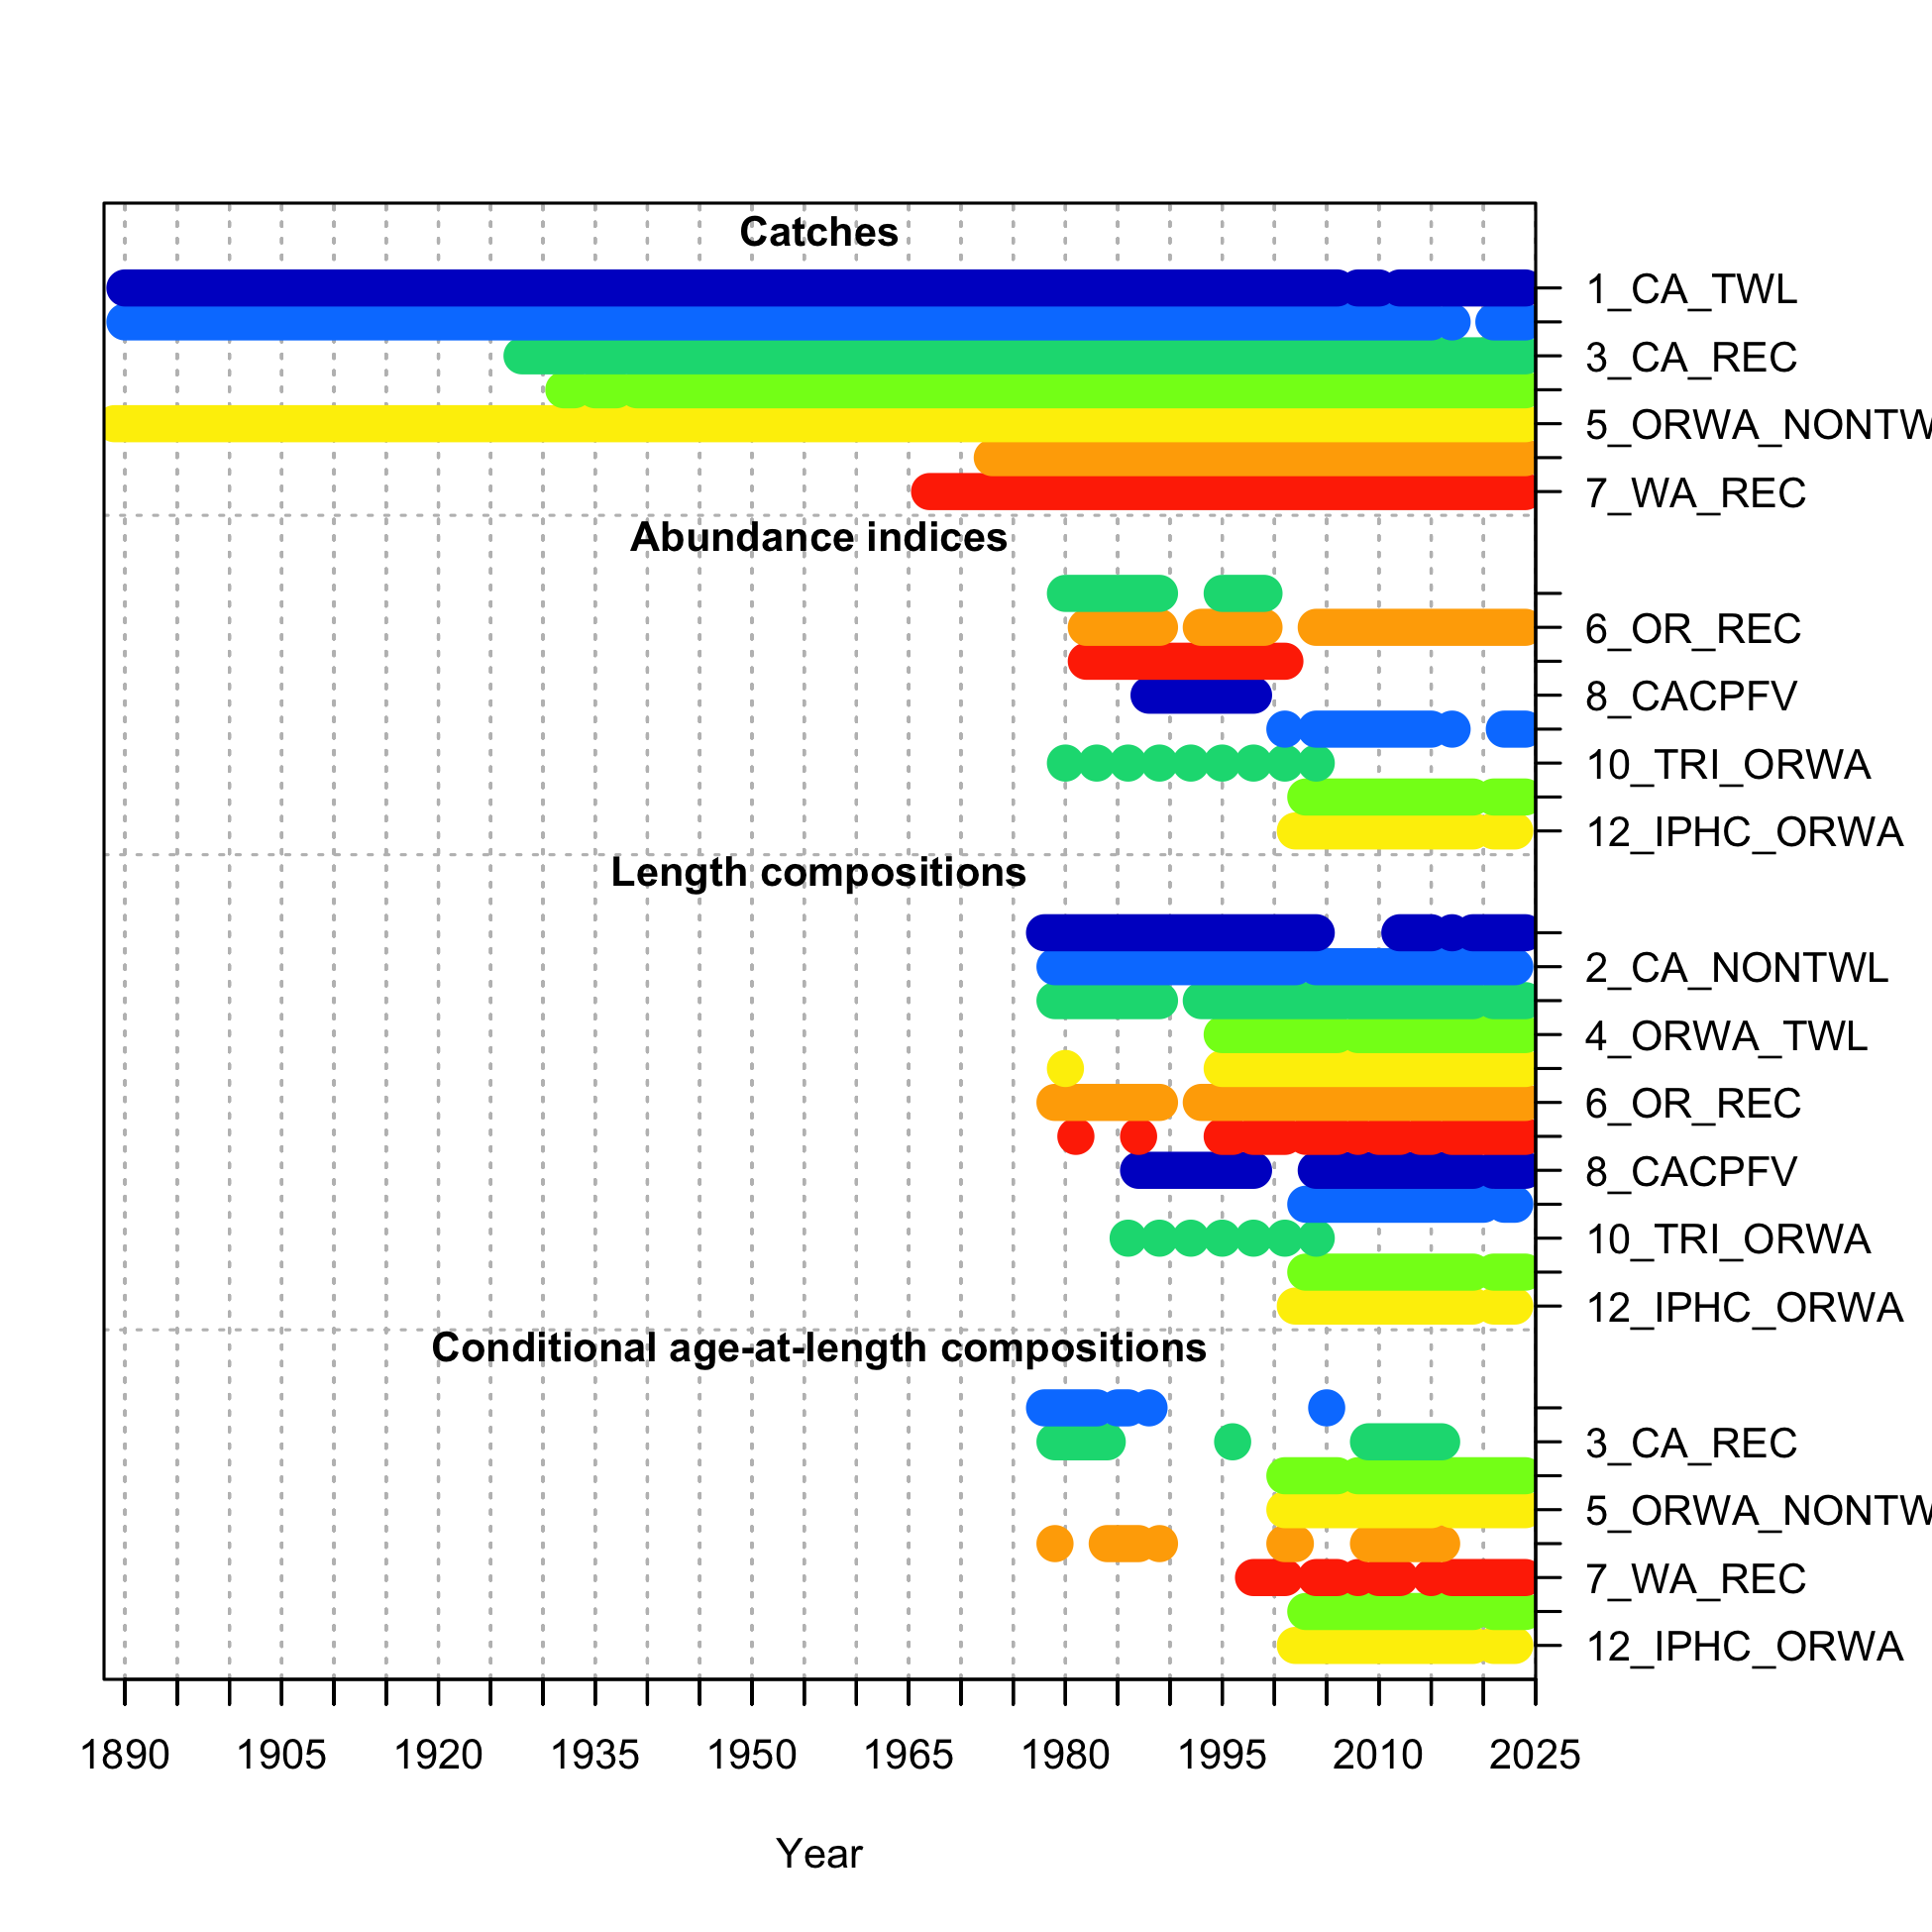
\includegraphics{figures/r4ss_plots/plots/data_plot.png}

}

\caption{\label{fig-data}Summary of data sources used in the base
model.}

\end{figure}%

\begin{figure}

\centering{

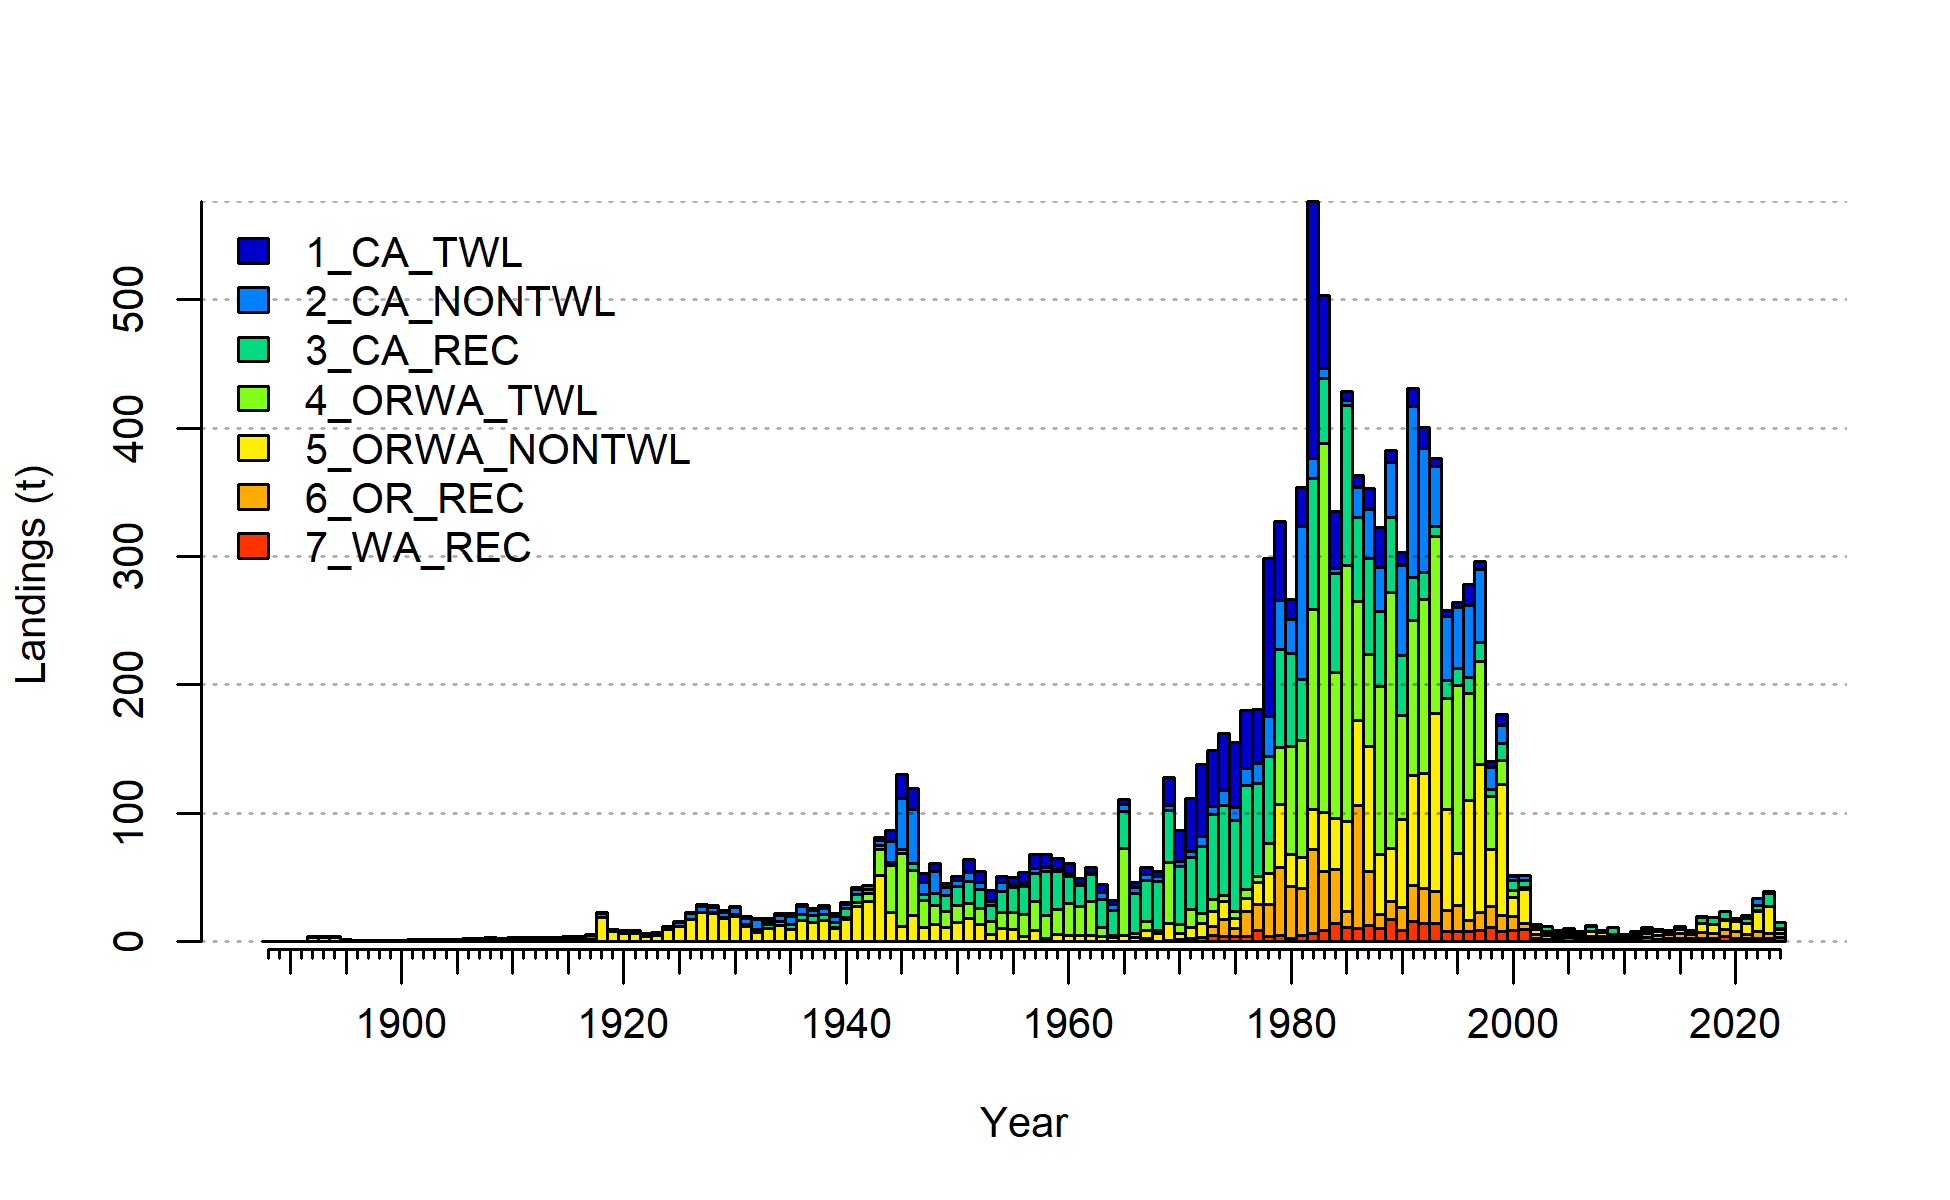
\includegraphics{figures/r4ss_plots/plots/catch2_landings_stacked.png}

}

\caption{\label{fig-catch}Yelloweye Rockfish landing history in metric
tons (mt) between 1889 and 2024 for each fleet.}

\end{figure}%

\begin{figure}

\centering{

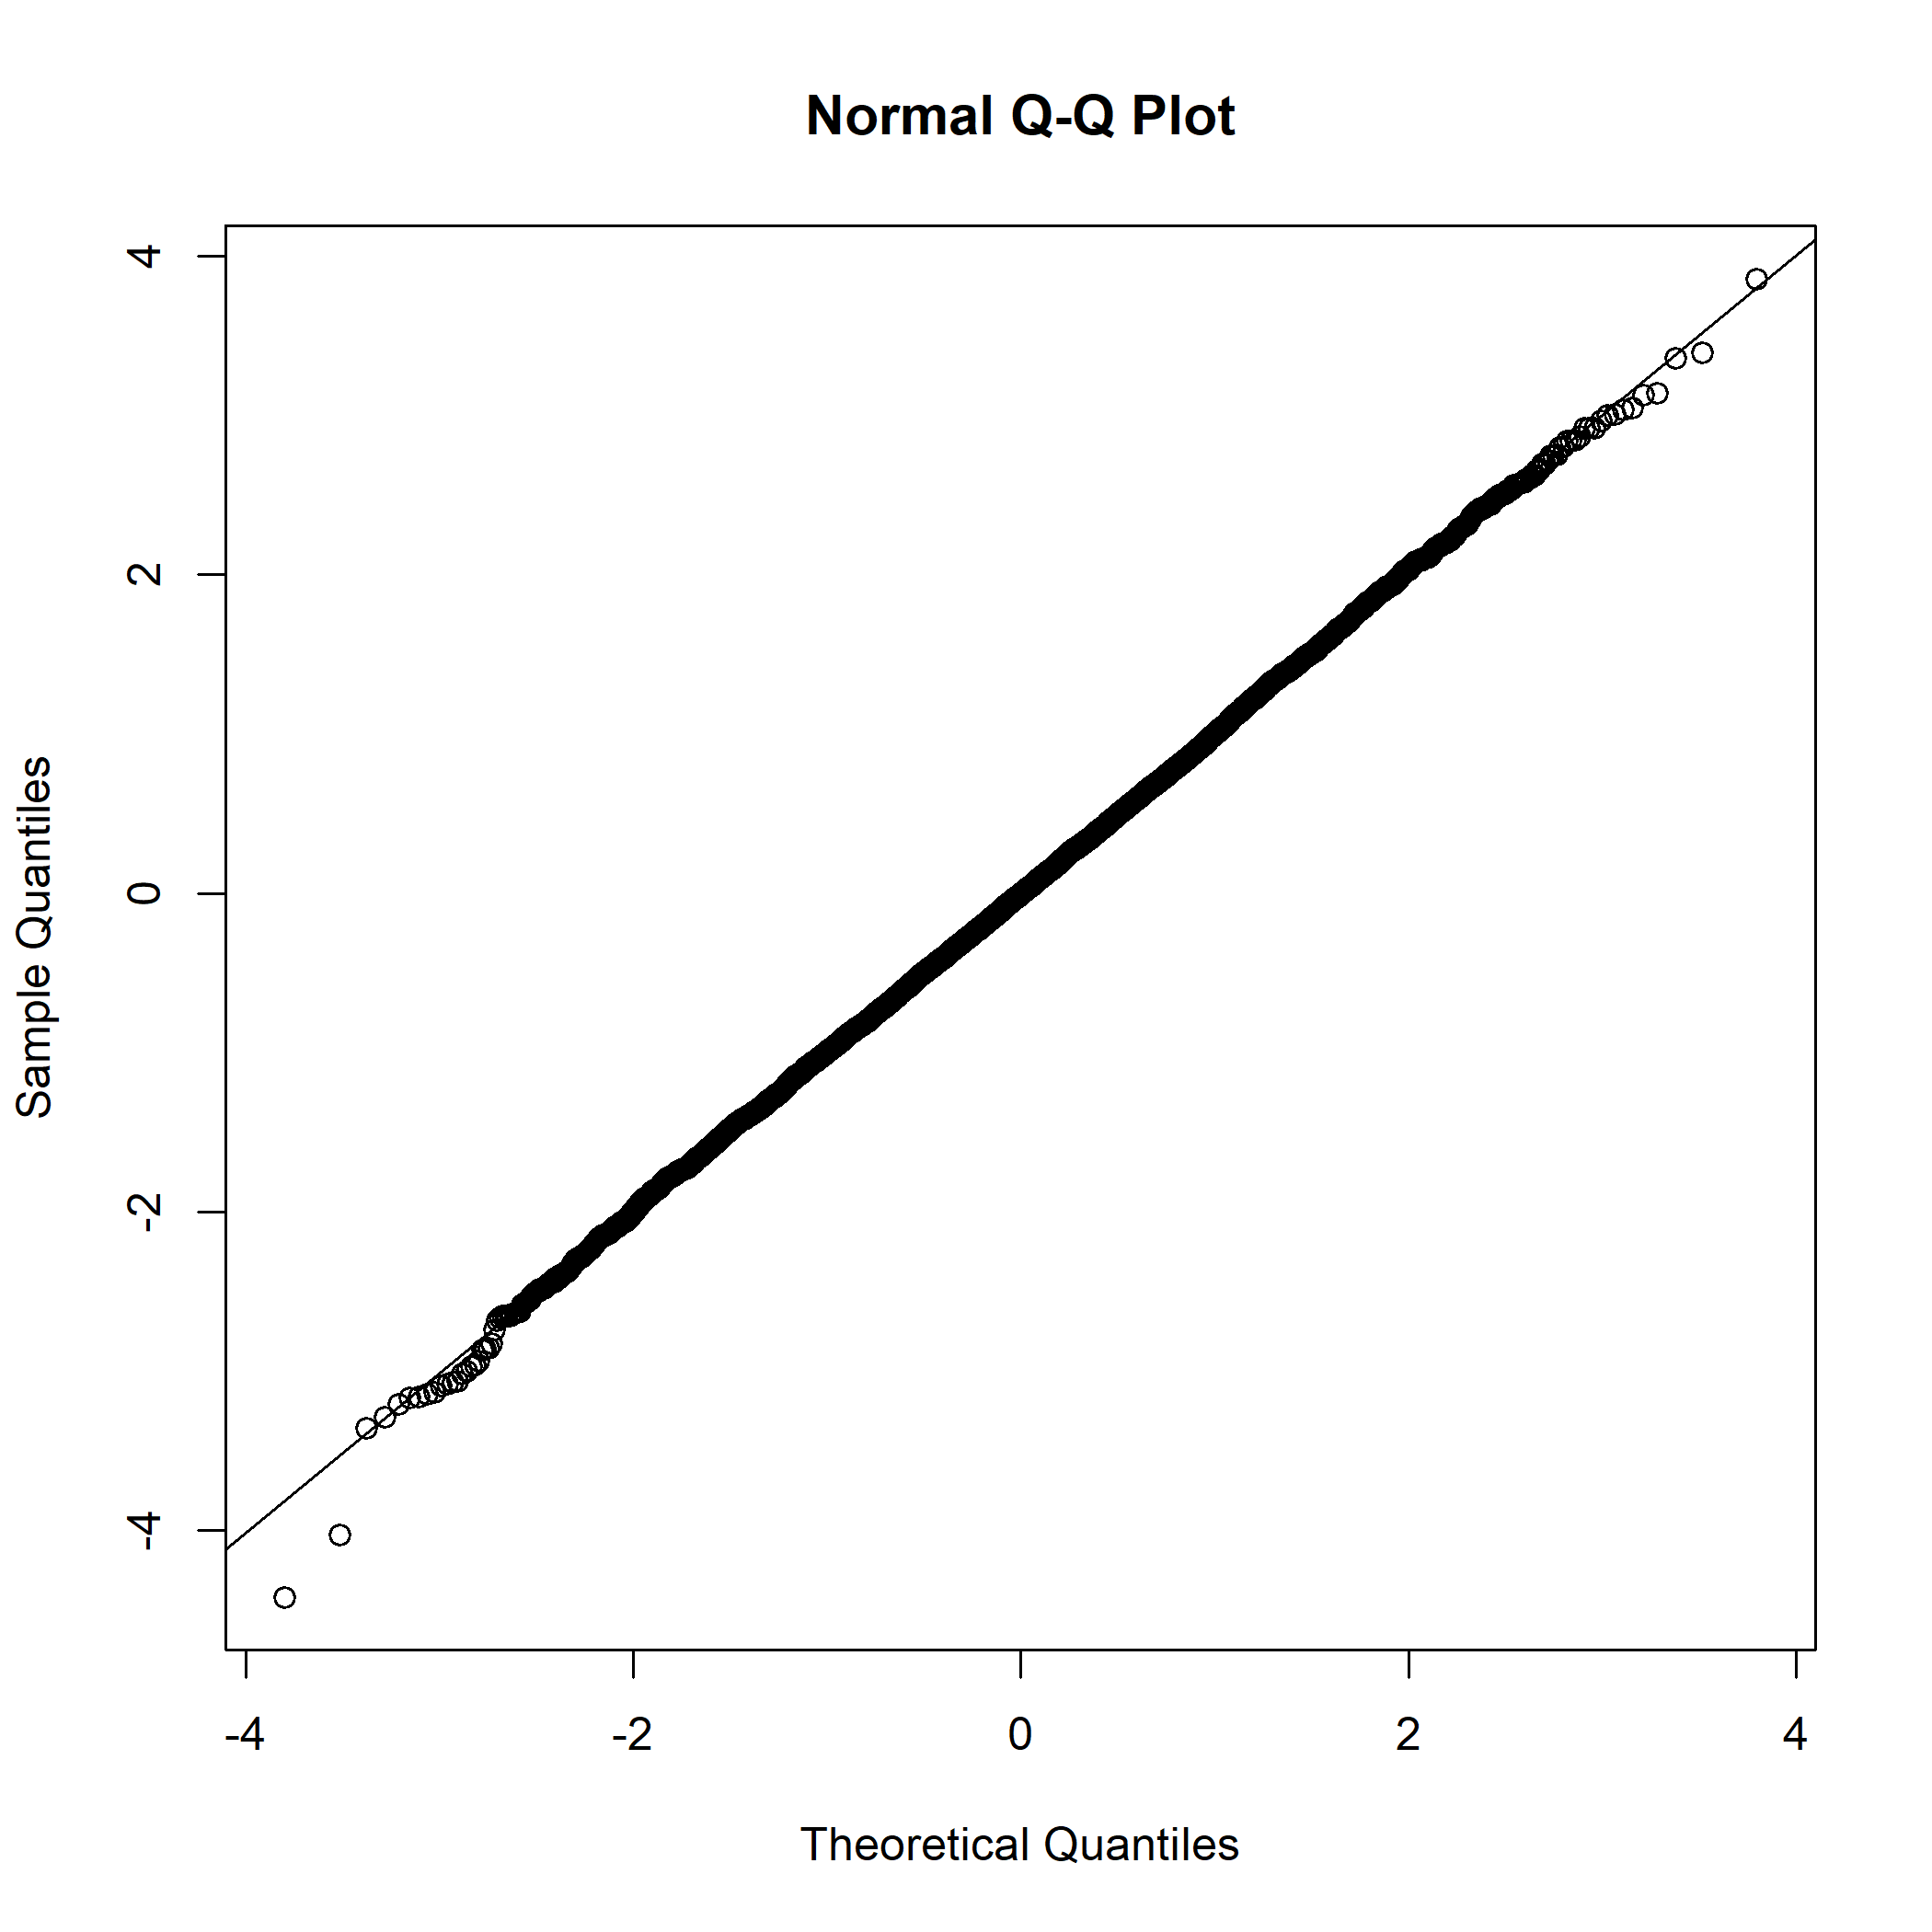
\includegraphics{figures/indices/ORFS_qq.png}

}

\caption{\label{fig-orfs_qqplot}Quantile-quantile plot for the sdmTMB
model fit for the Oregon Onboard Observer (ORFS) index.}

\end{figure}%

\begin{figure}

\centering{

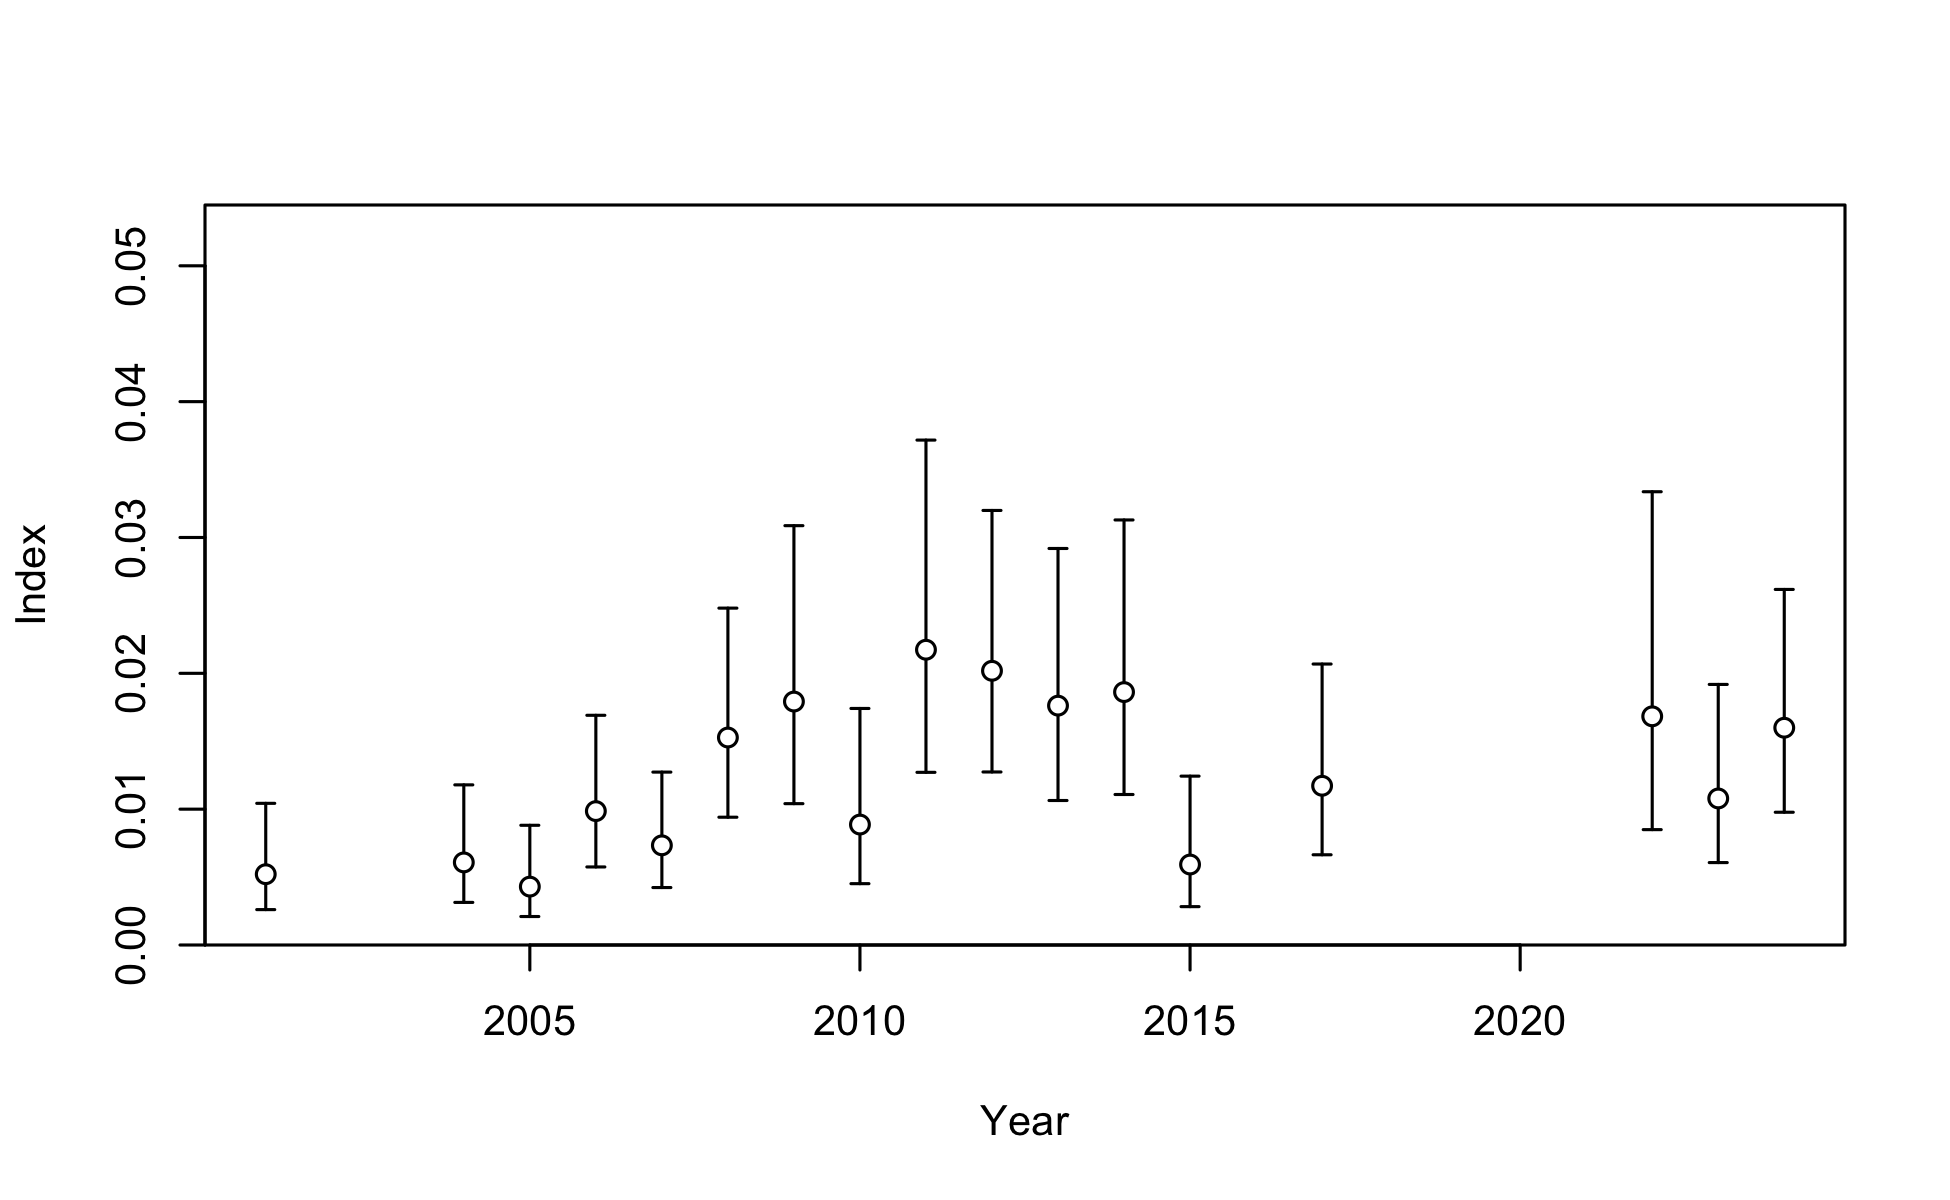
\includegraphics{figures/r4ss_plots/plots/index1_cpuedata_9_OR_RECOB.png}

}

\caption{\label{fig-ORFS_index}Annual relative index of abundance for
the Oregon Onboard Observer (ORFS) index.}

\end{figure}%

\begin{figure}

\centering{

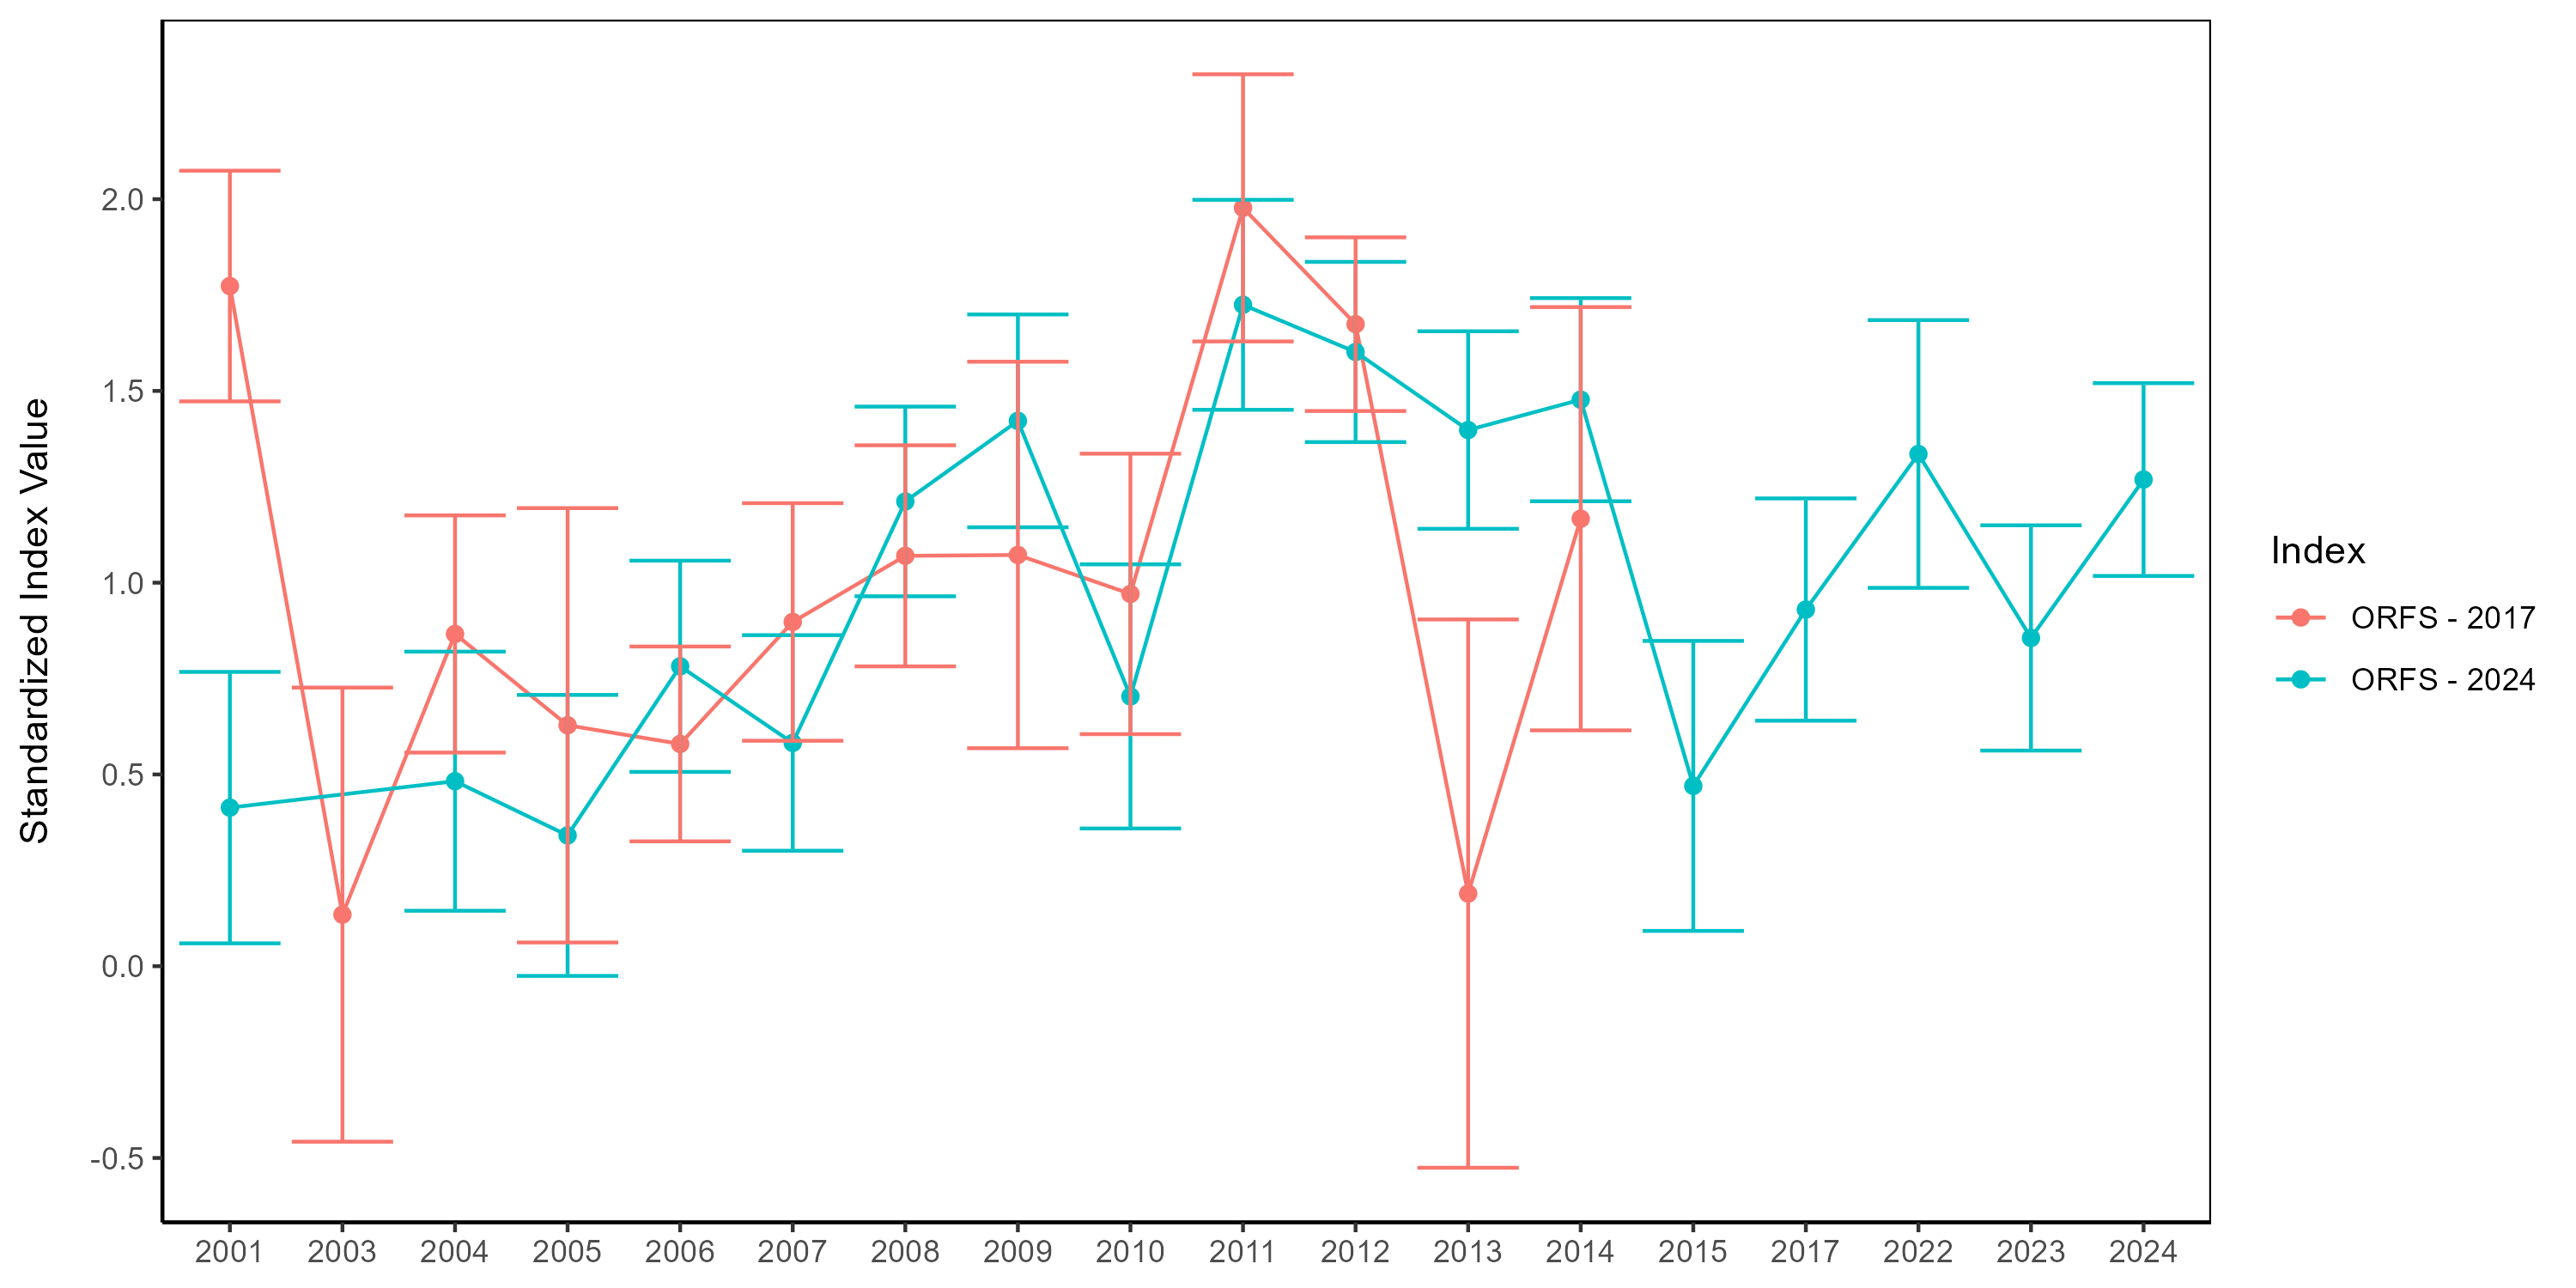
\includegraphics{figures/indices/ORFS index comparison_errbars.png}

}

\caption{\label{fig-ORFS_comp}Comparison of Oregon Onboard Observer
indices from the 2017 and the current assessment.}

\end{figure}%

\begin{figure}

\centering{

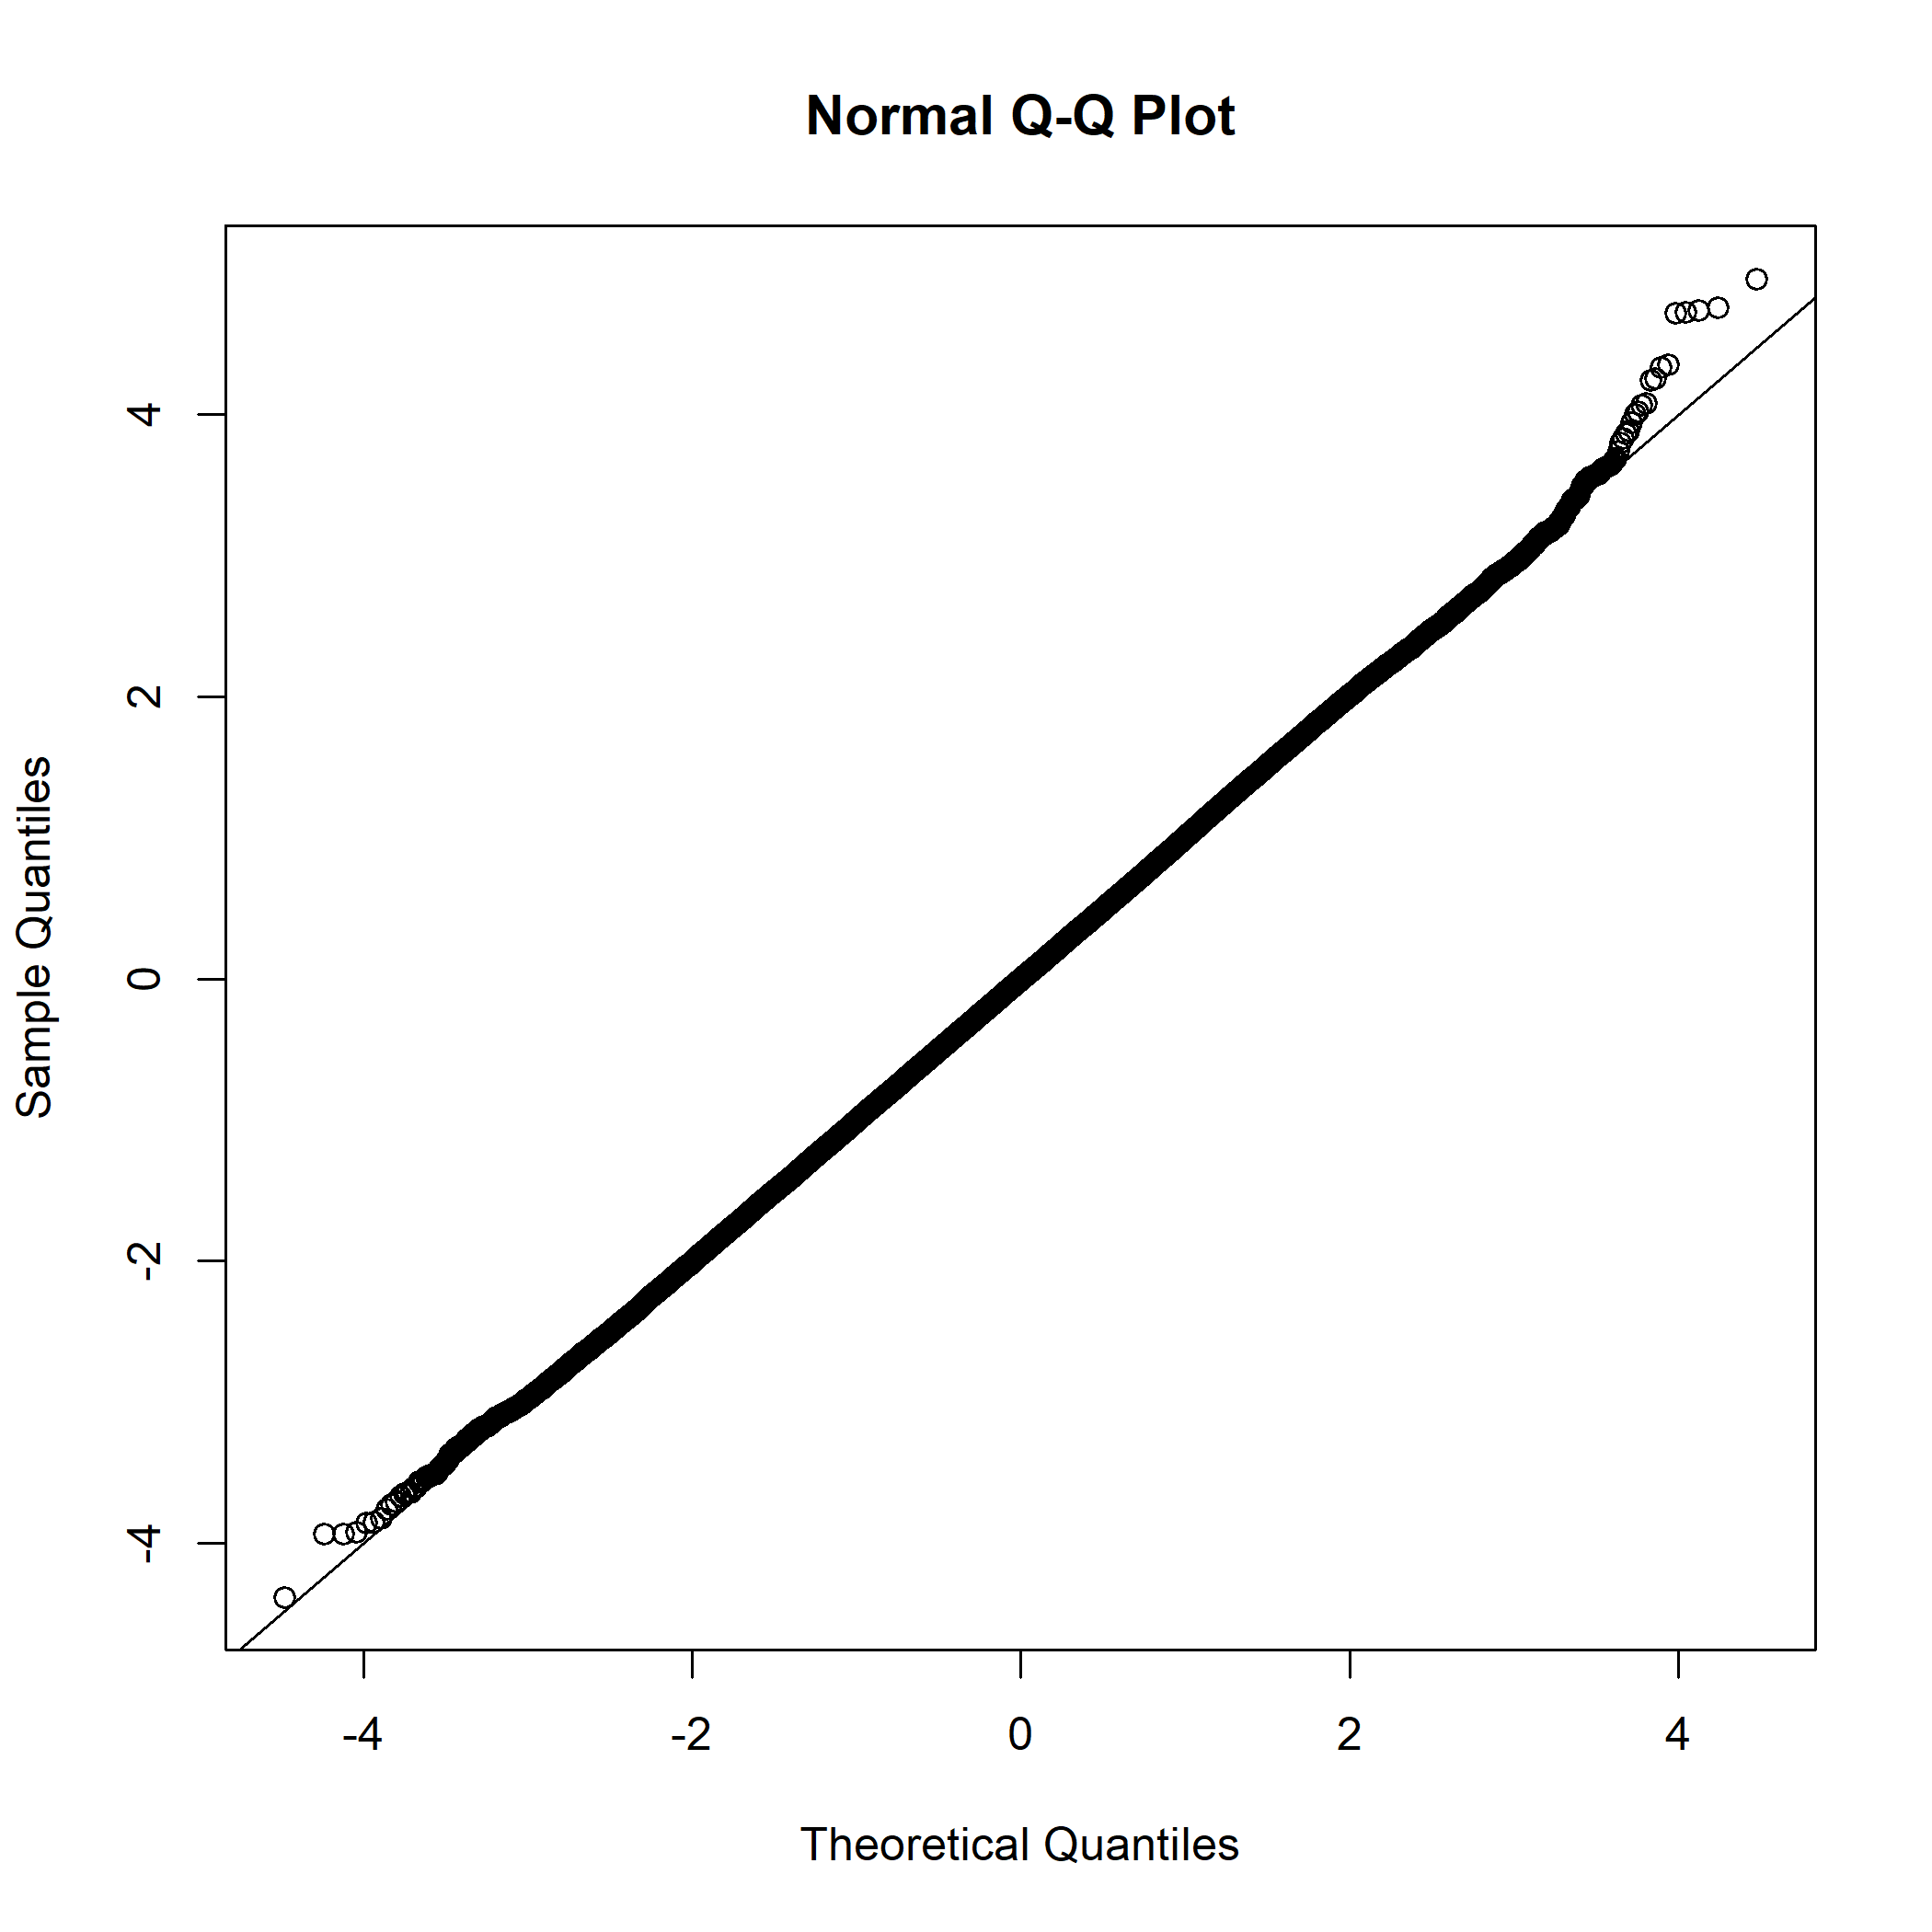
\includegraphics{figures/indices/ORBS_qq.png}

}

\caption{\label{fig-orbs_qq}Quantile-quantile plot for the sdmTMB model
fit for the updated portion of the Oregon recreational (ORBS) index.}

\end{figure}%

\begin{figure}

\centering{

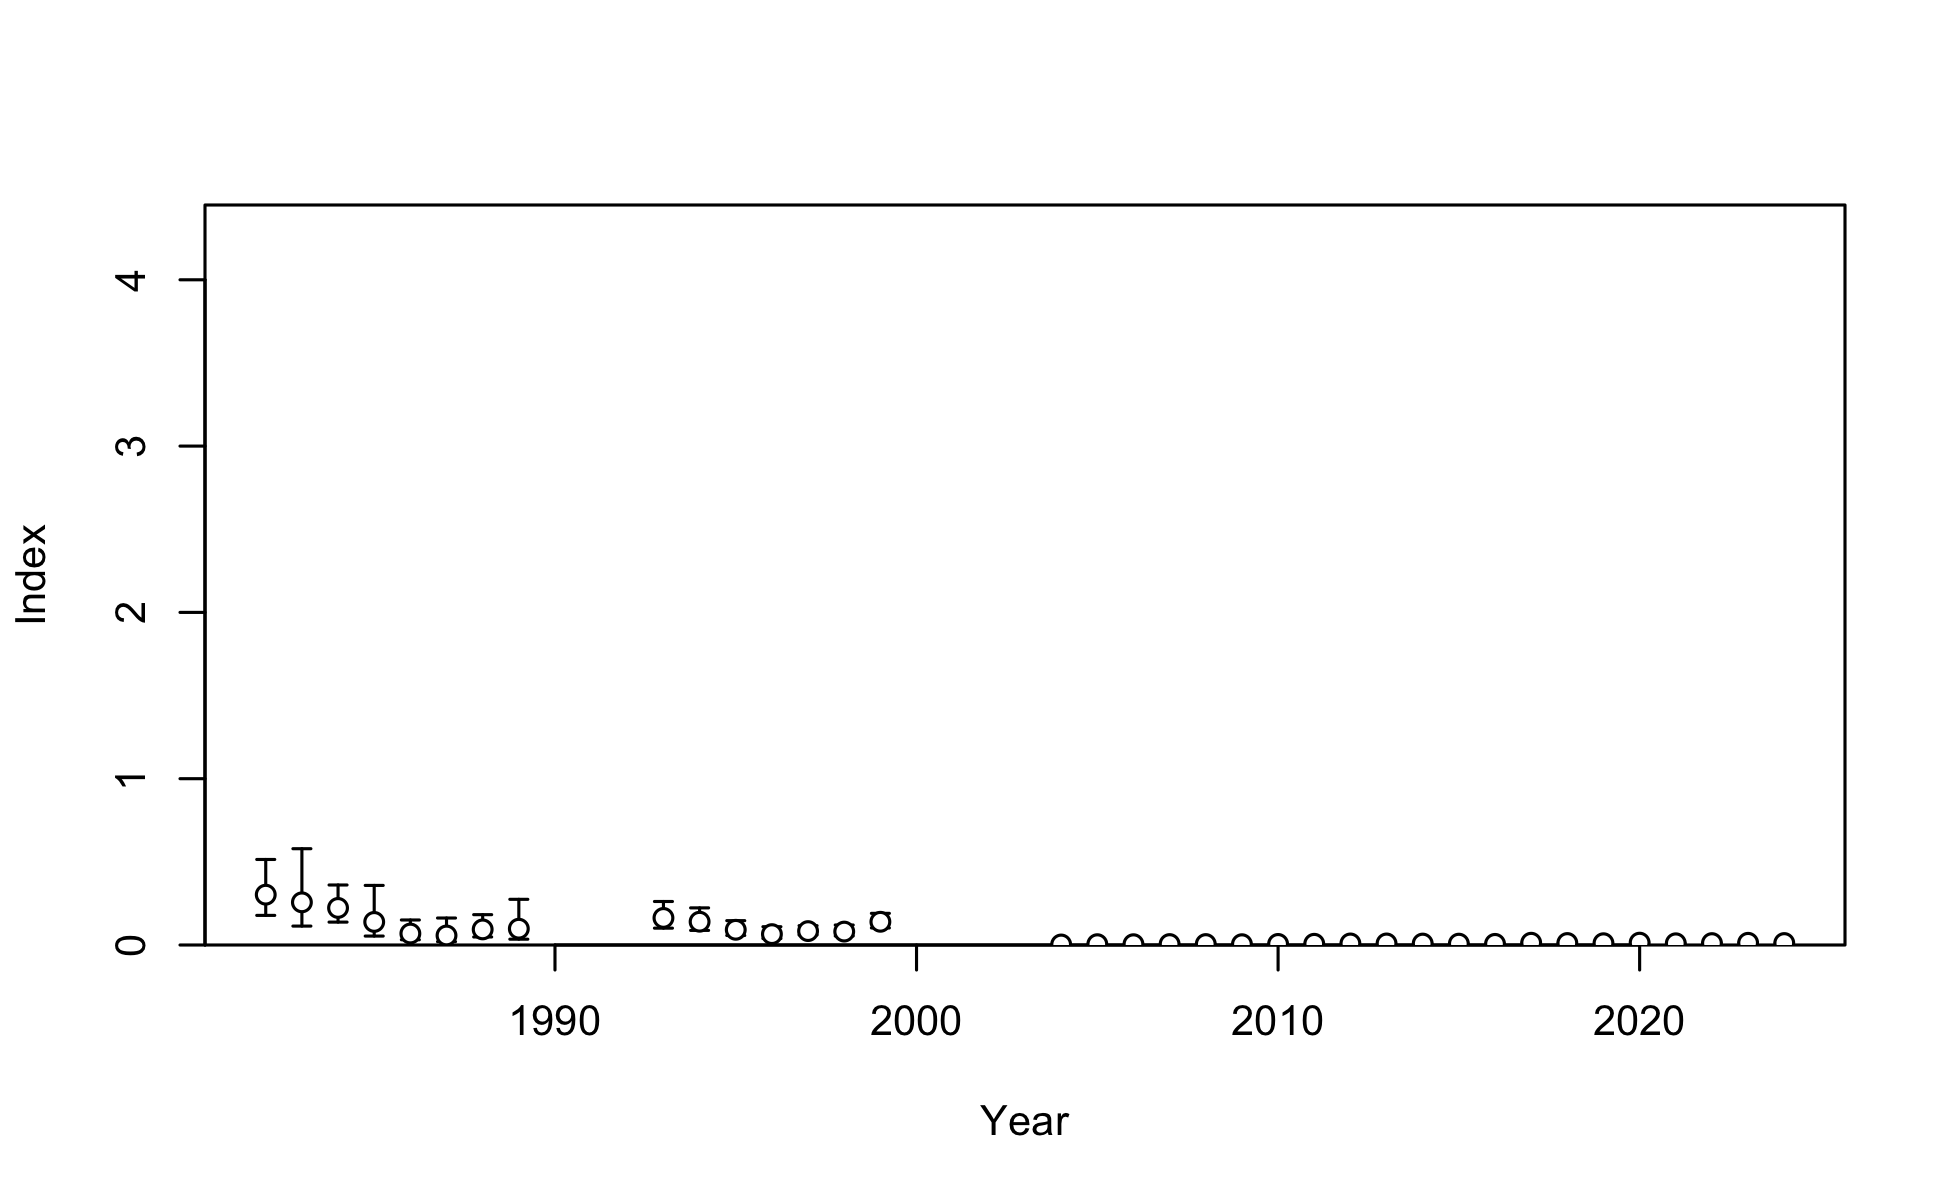
\includegraphics{figures/r4ss_plots/plots/index1_cpuedata_6_OR_REC.png}

}

\caption{\label{fig-ORBS_index}Annual relative index of abundance for
the Oregon recreational index, including both MRFSS (1980 - 1999) and
ORBS (2004 - 2024) indices.}

\end{figure}%

\clearpage

\begin{figure}

\centering{

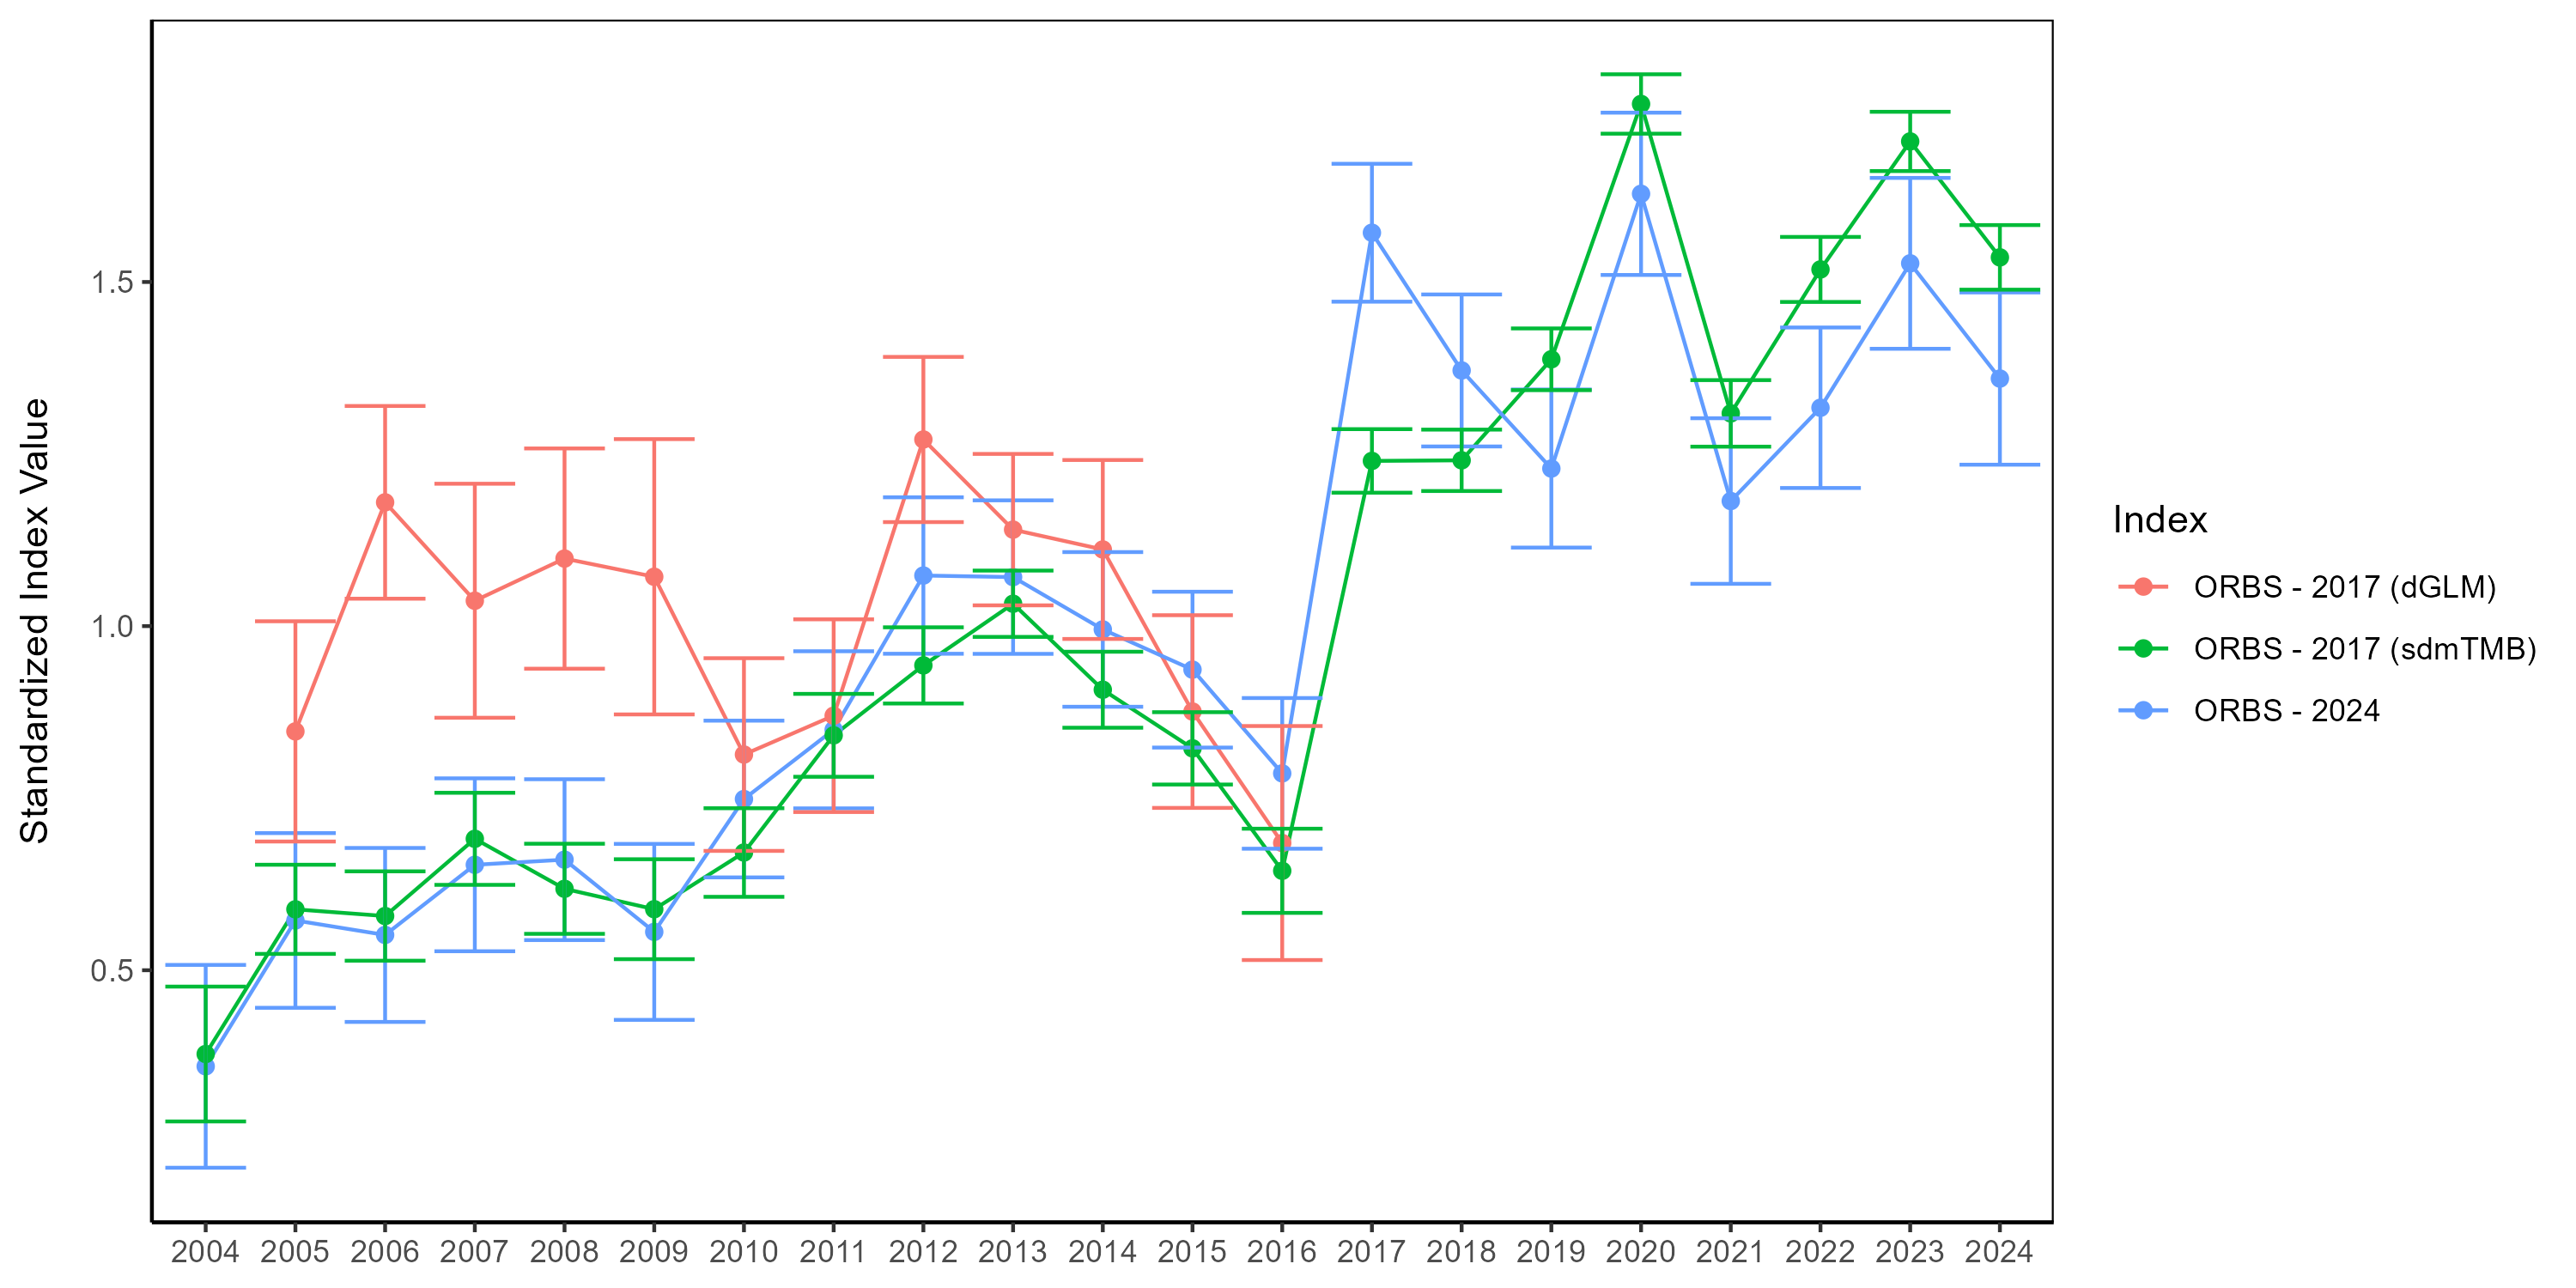
\includegraphics{figures/indices/ORBS index comparison_ORBSonly_errbars.png}

}

\caption{\label{fig-ORBS_comp}Comparison of the 2017 ORBS index
(delta-GLM), the 2017 ORBS model structure (with the current dataset and
implemented in sdmTMB), and the current ORBS index (sdmTMB).}

\end{figure}%

\begin{figure}

\centering{

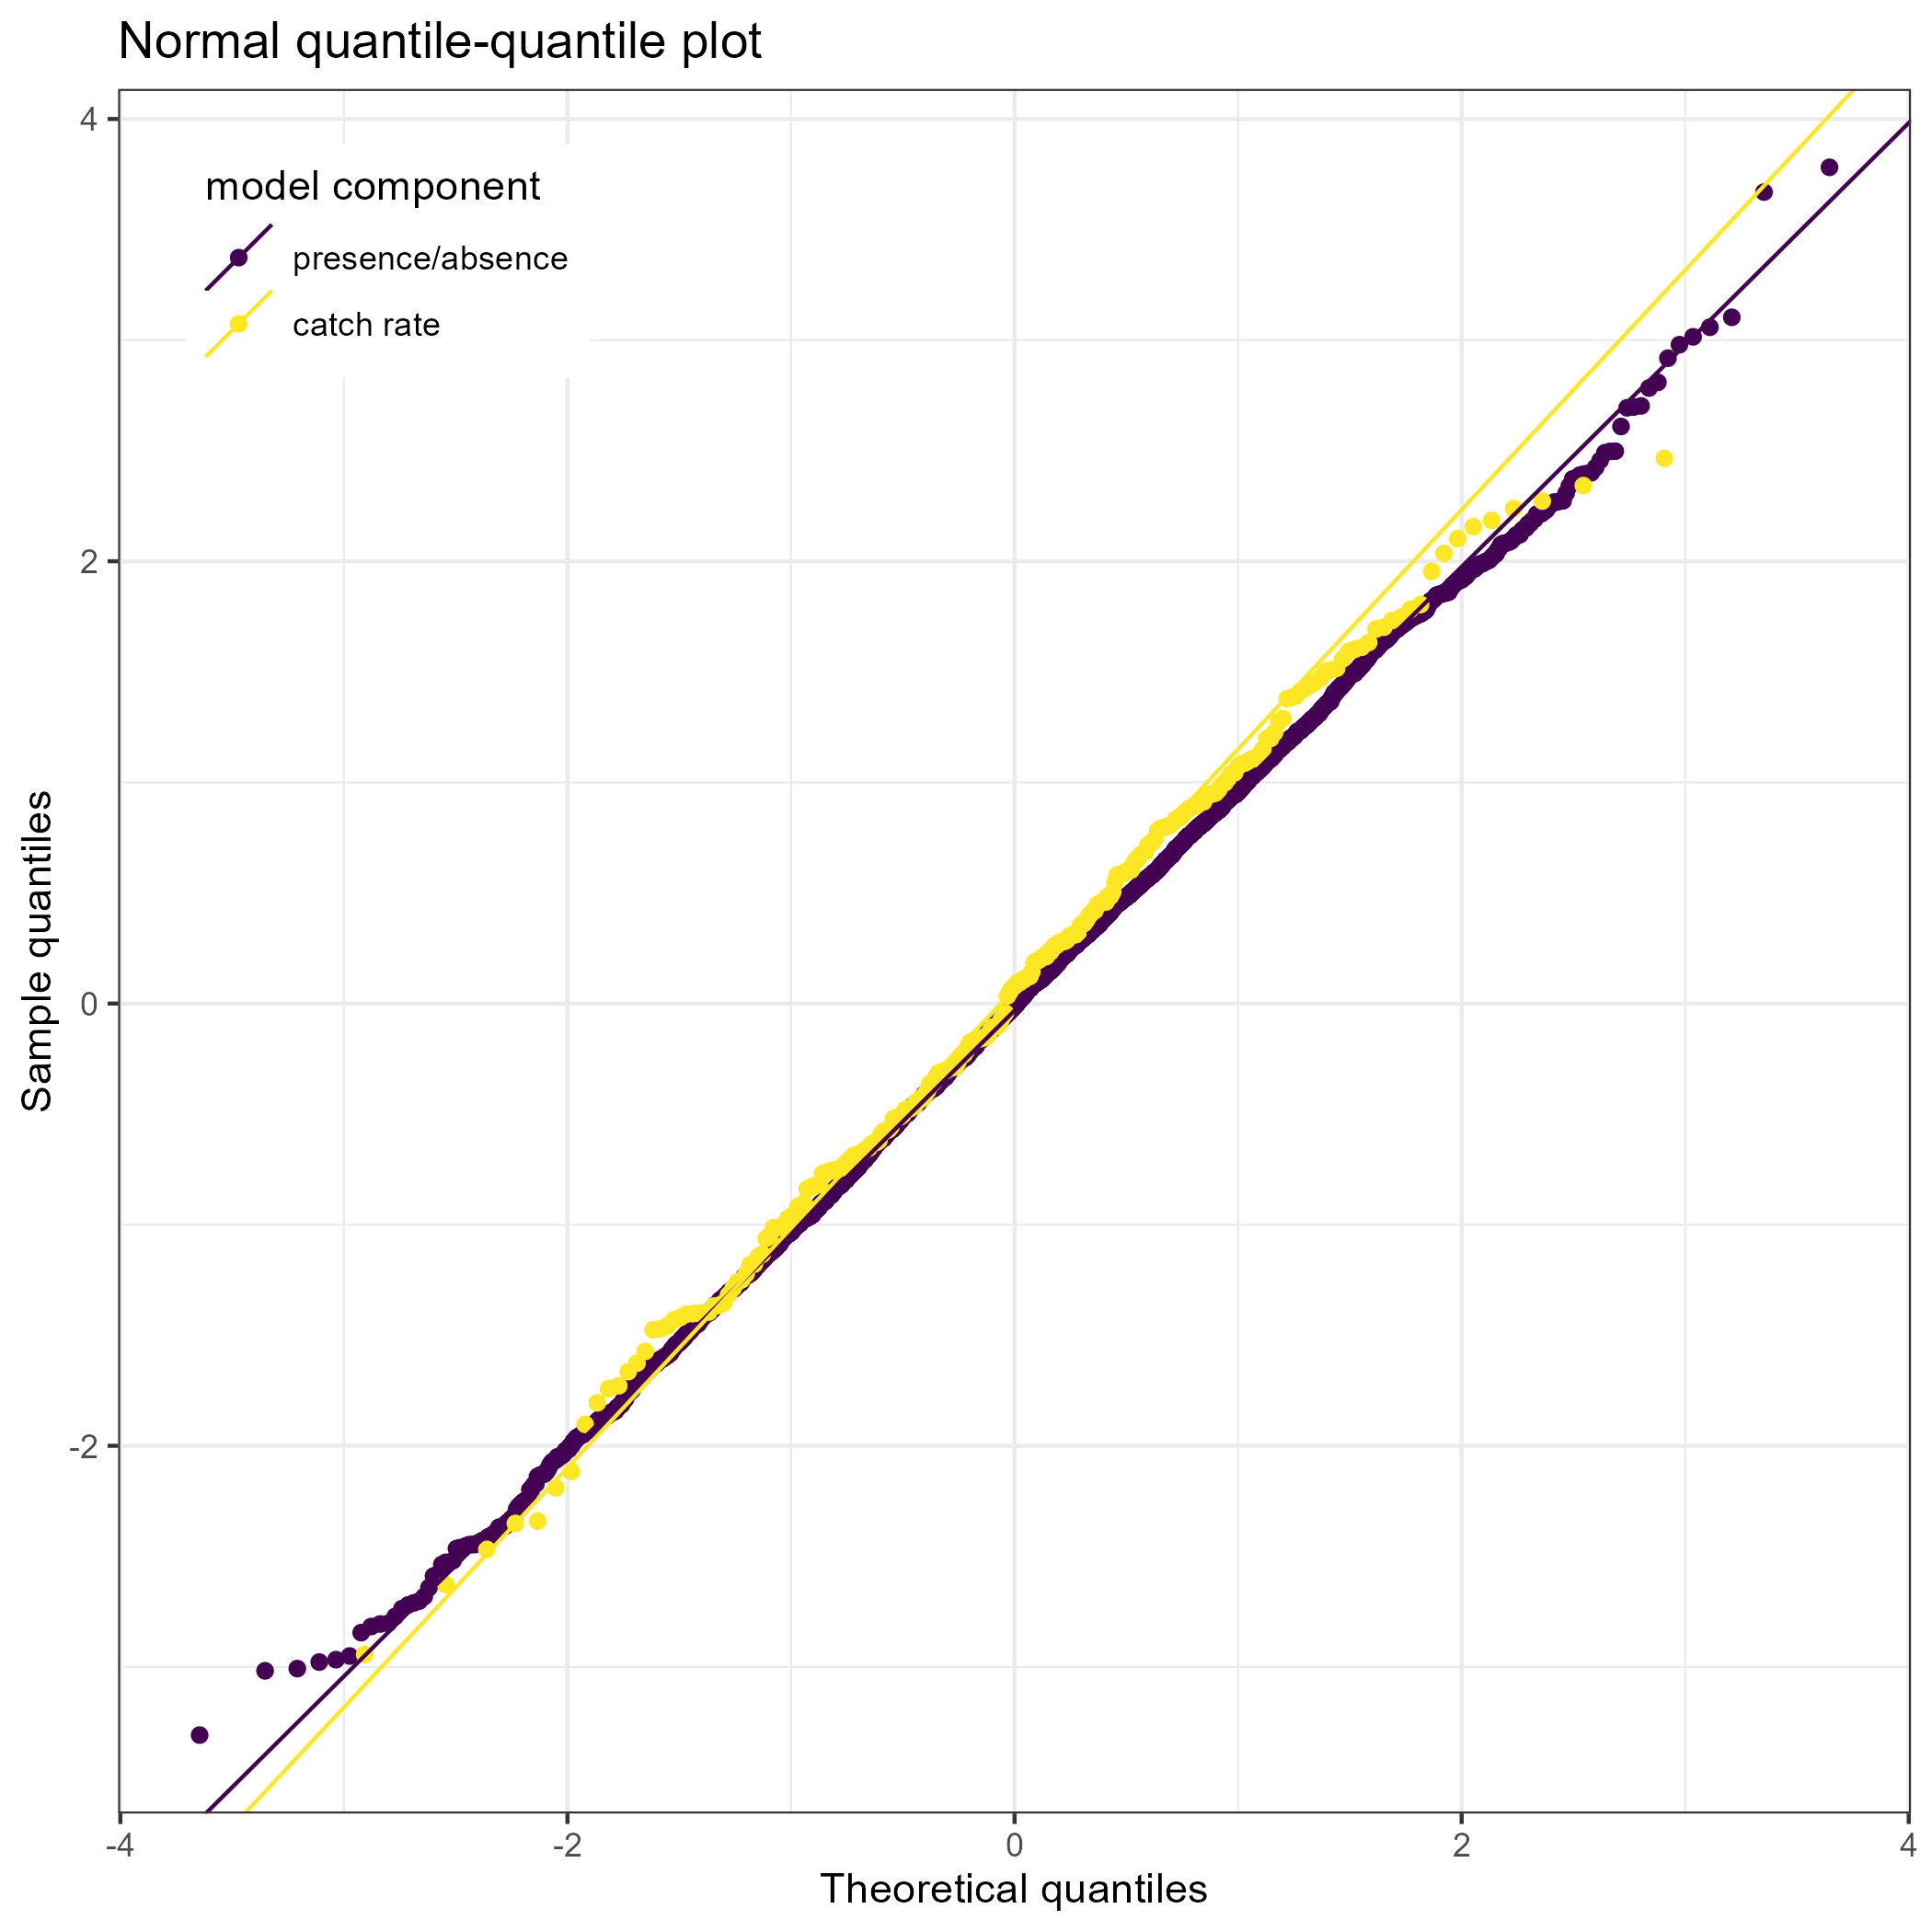
\includegraphics{figures/indices/wcgbts_qq.png}

}

\caption{\label{fig-wcgbts_qq}Quantile-quantile plot for the sdmTMB
model fit for the NWFSC West Coast Groundfish Bottom Trawl Survey
(WCGBTS) index.}

\end{figure}%

\begin{figure}

\centering{

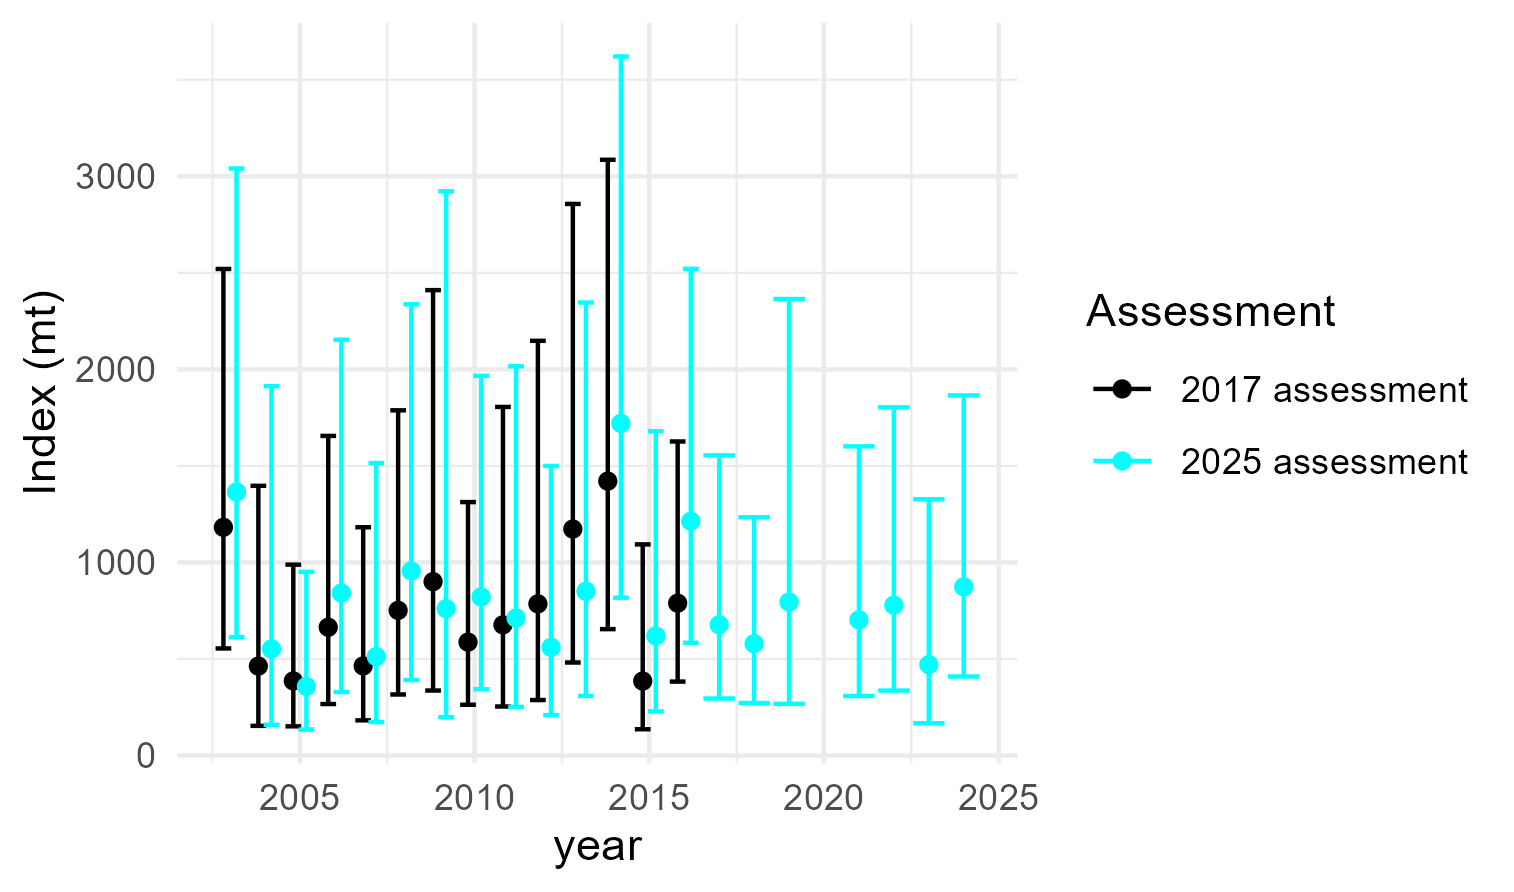
\includegraphics{figures/indices/wcgbts_index_comparison.png}

}

\caption{\label{fig-wcgbtsindexcomparison}Comparison of the 2017 NWFSC
West Coast Groundfish Bottom Trawl Survey (WCGBTS) and the current WCBTS
index of abundance.}

\end{figure}%

\begin{figure}

\centering{

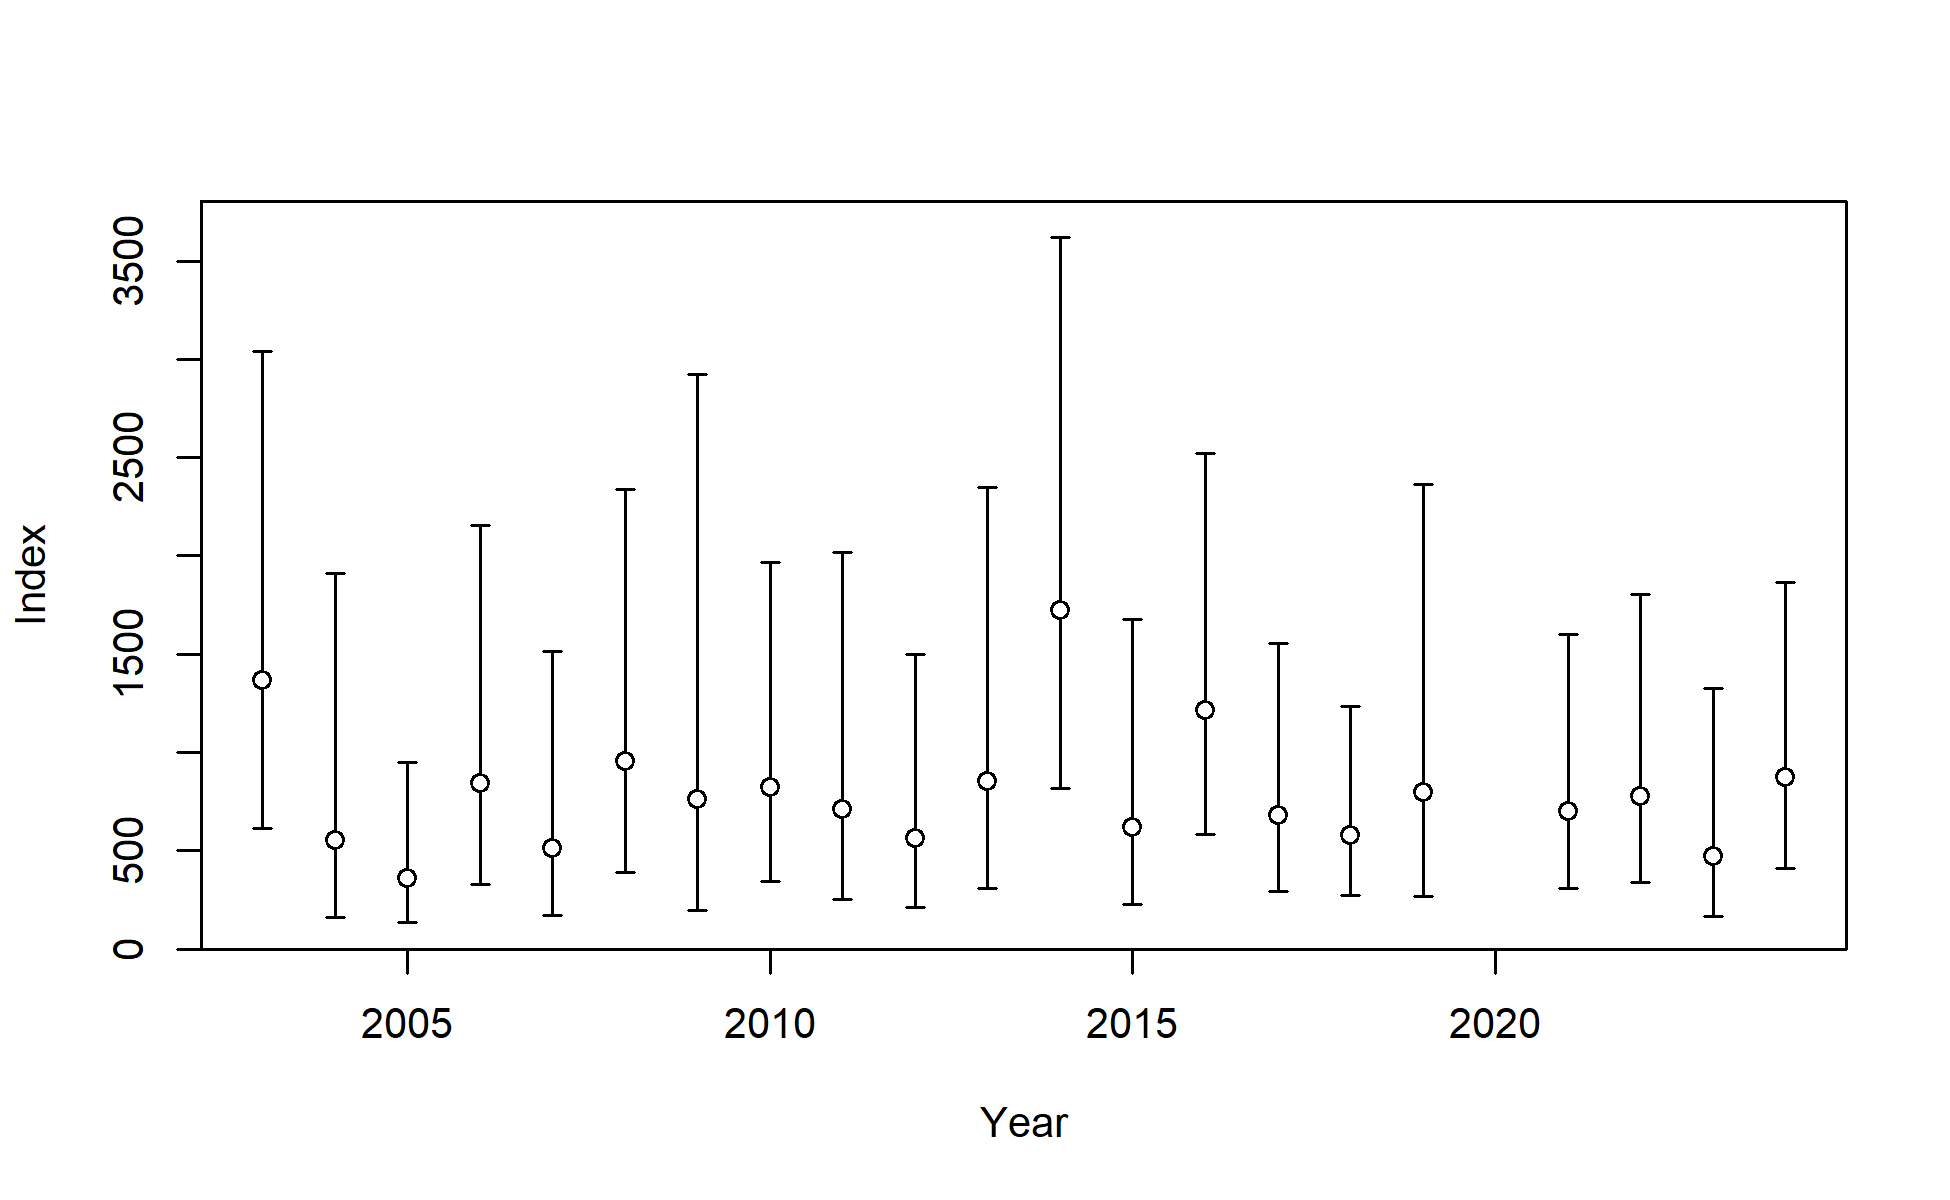
\includegraphics{figures/r4ss_plots/plots/index1_cpuedata_11_NWFSC_ORWA.png}

}

\caption{\label{fig-wcgbtsindex}Annual relative index of abundance for
the West Coast Groundfish Bottom Trawl Survey (WCGBTS).}

\end{figure}%

\begin{figure}

\centering{

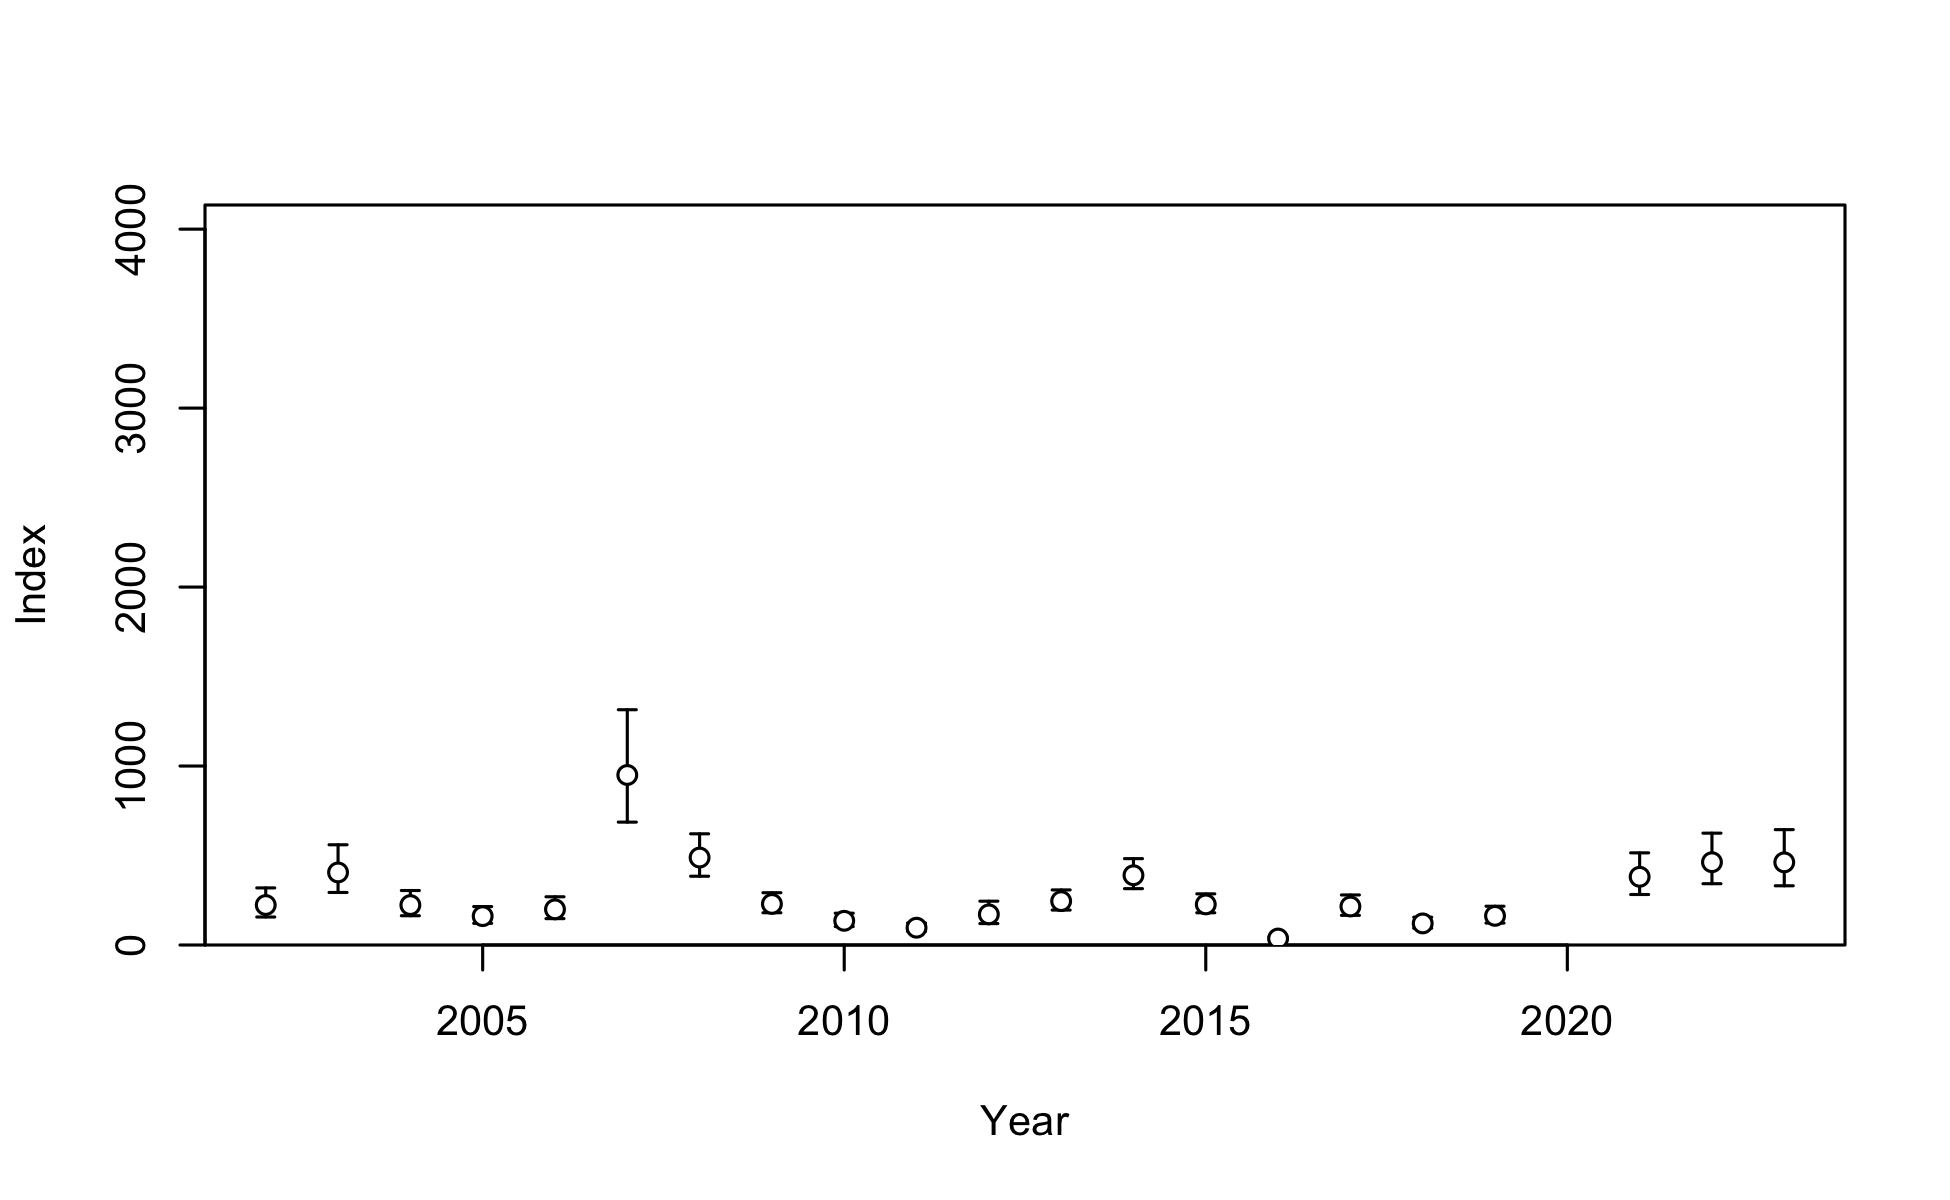
\includegraphics{figures/r4ss_plots/plots/index1_cpuedata_12_IPHC_ORWA.png}

}

\caption{\label{fig-IPHC_index}Annual relative index of abundance for
the IPHC longline survey.}

\end{figure}%

\begin{figure}

\centering{

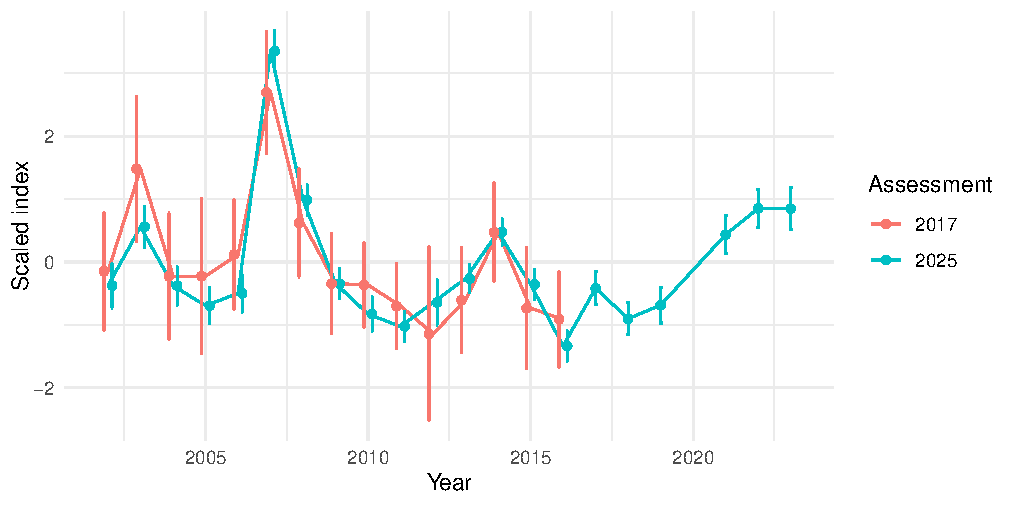
\includegraphics{figures/indices/IPHC_index_comparison.pdf}

}

\caption{\label{fig-IPHC_comparison}Comparison of the 2017 and the
current IPHC index of abundance.}

\end{figure}%

\begin{figure}

\centering{

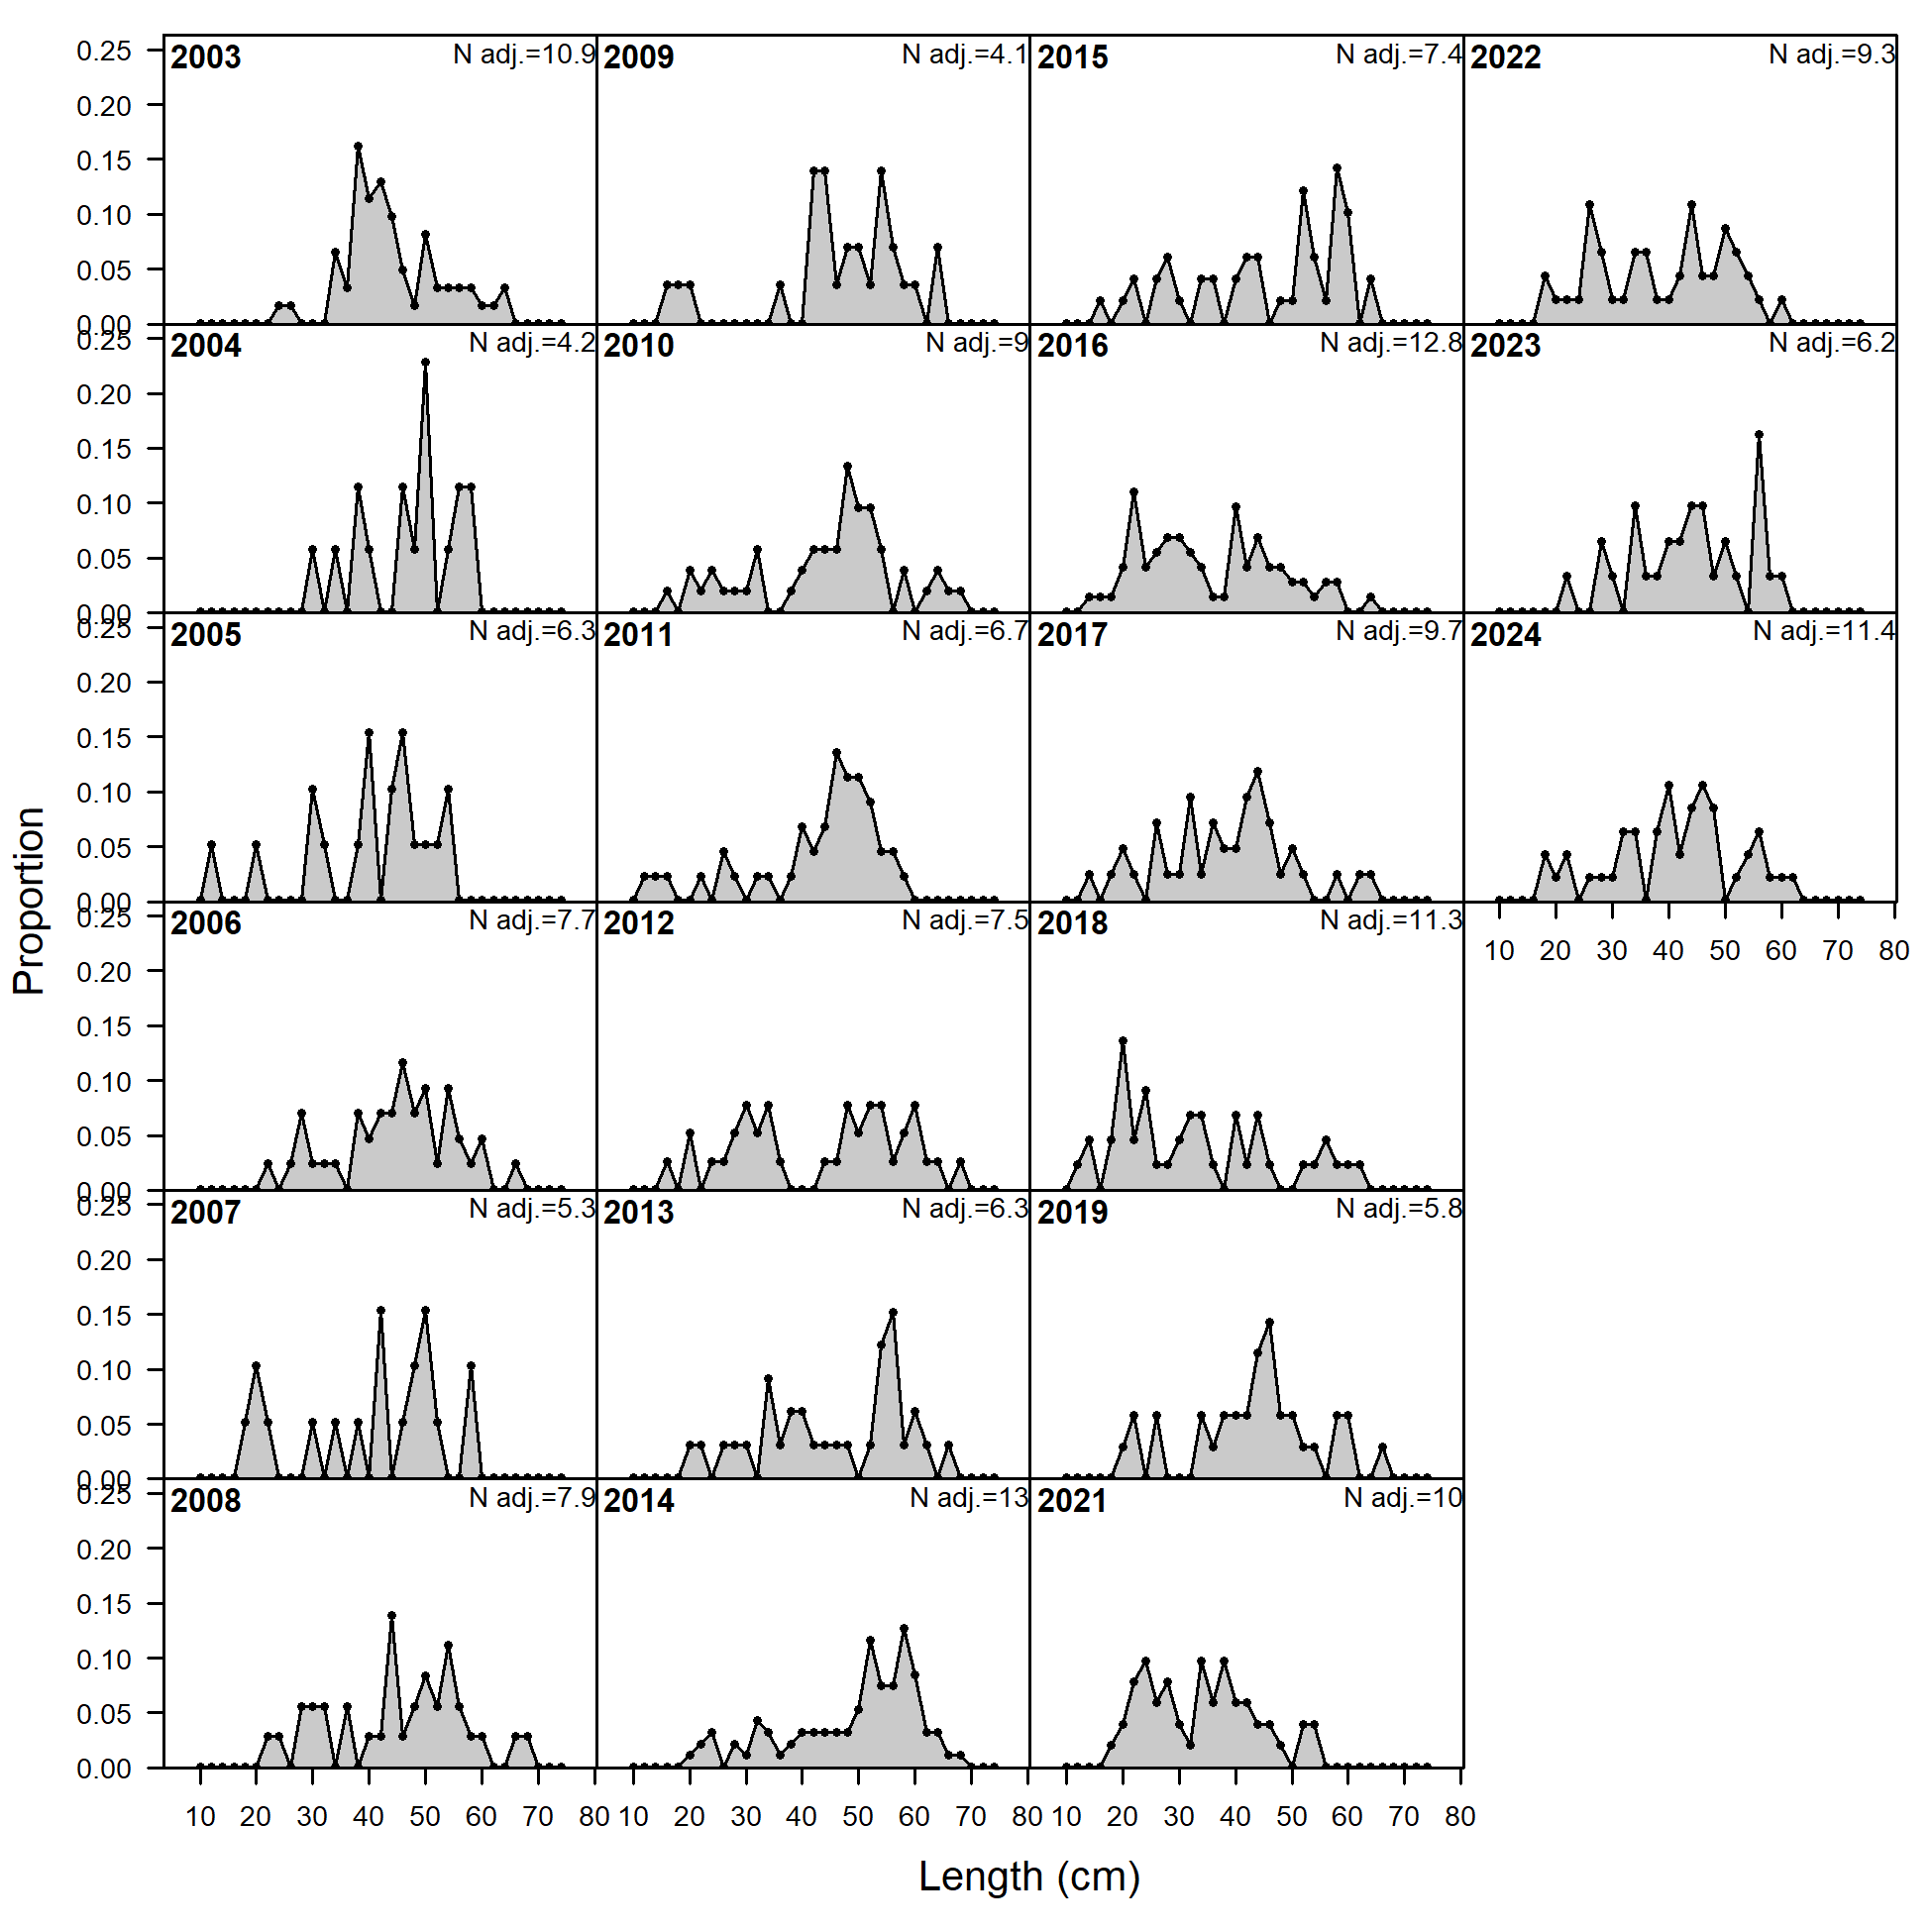
\includegraphics{figures/r4ss_plots/plots/comp_lendat_flt11mkt0.png}

}

\caption{\label{fig-NWFSC_lencomps}Annual length composition data for
the WCBTS.}

\end{figure}%

\begin{figure}

\centering{

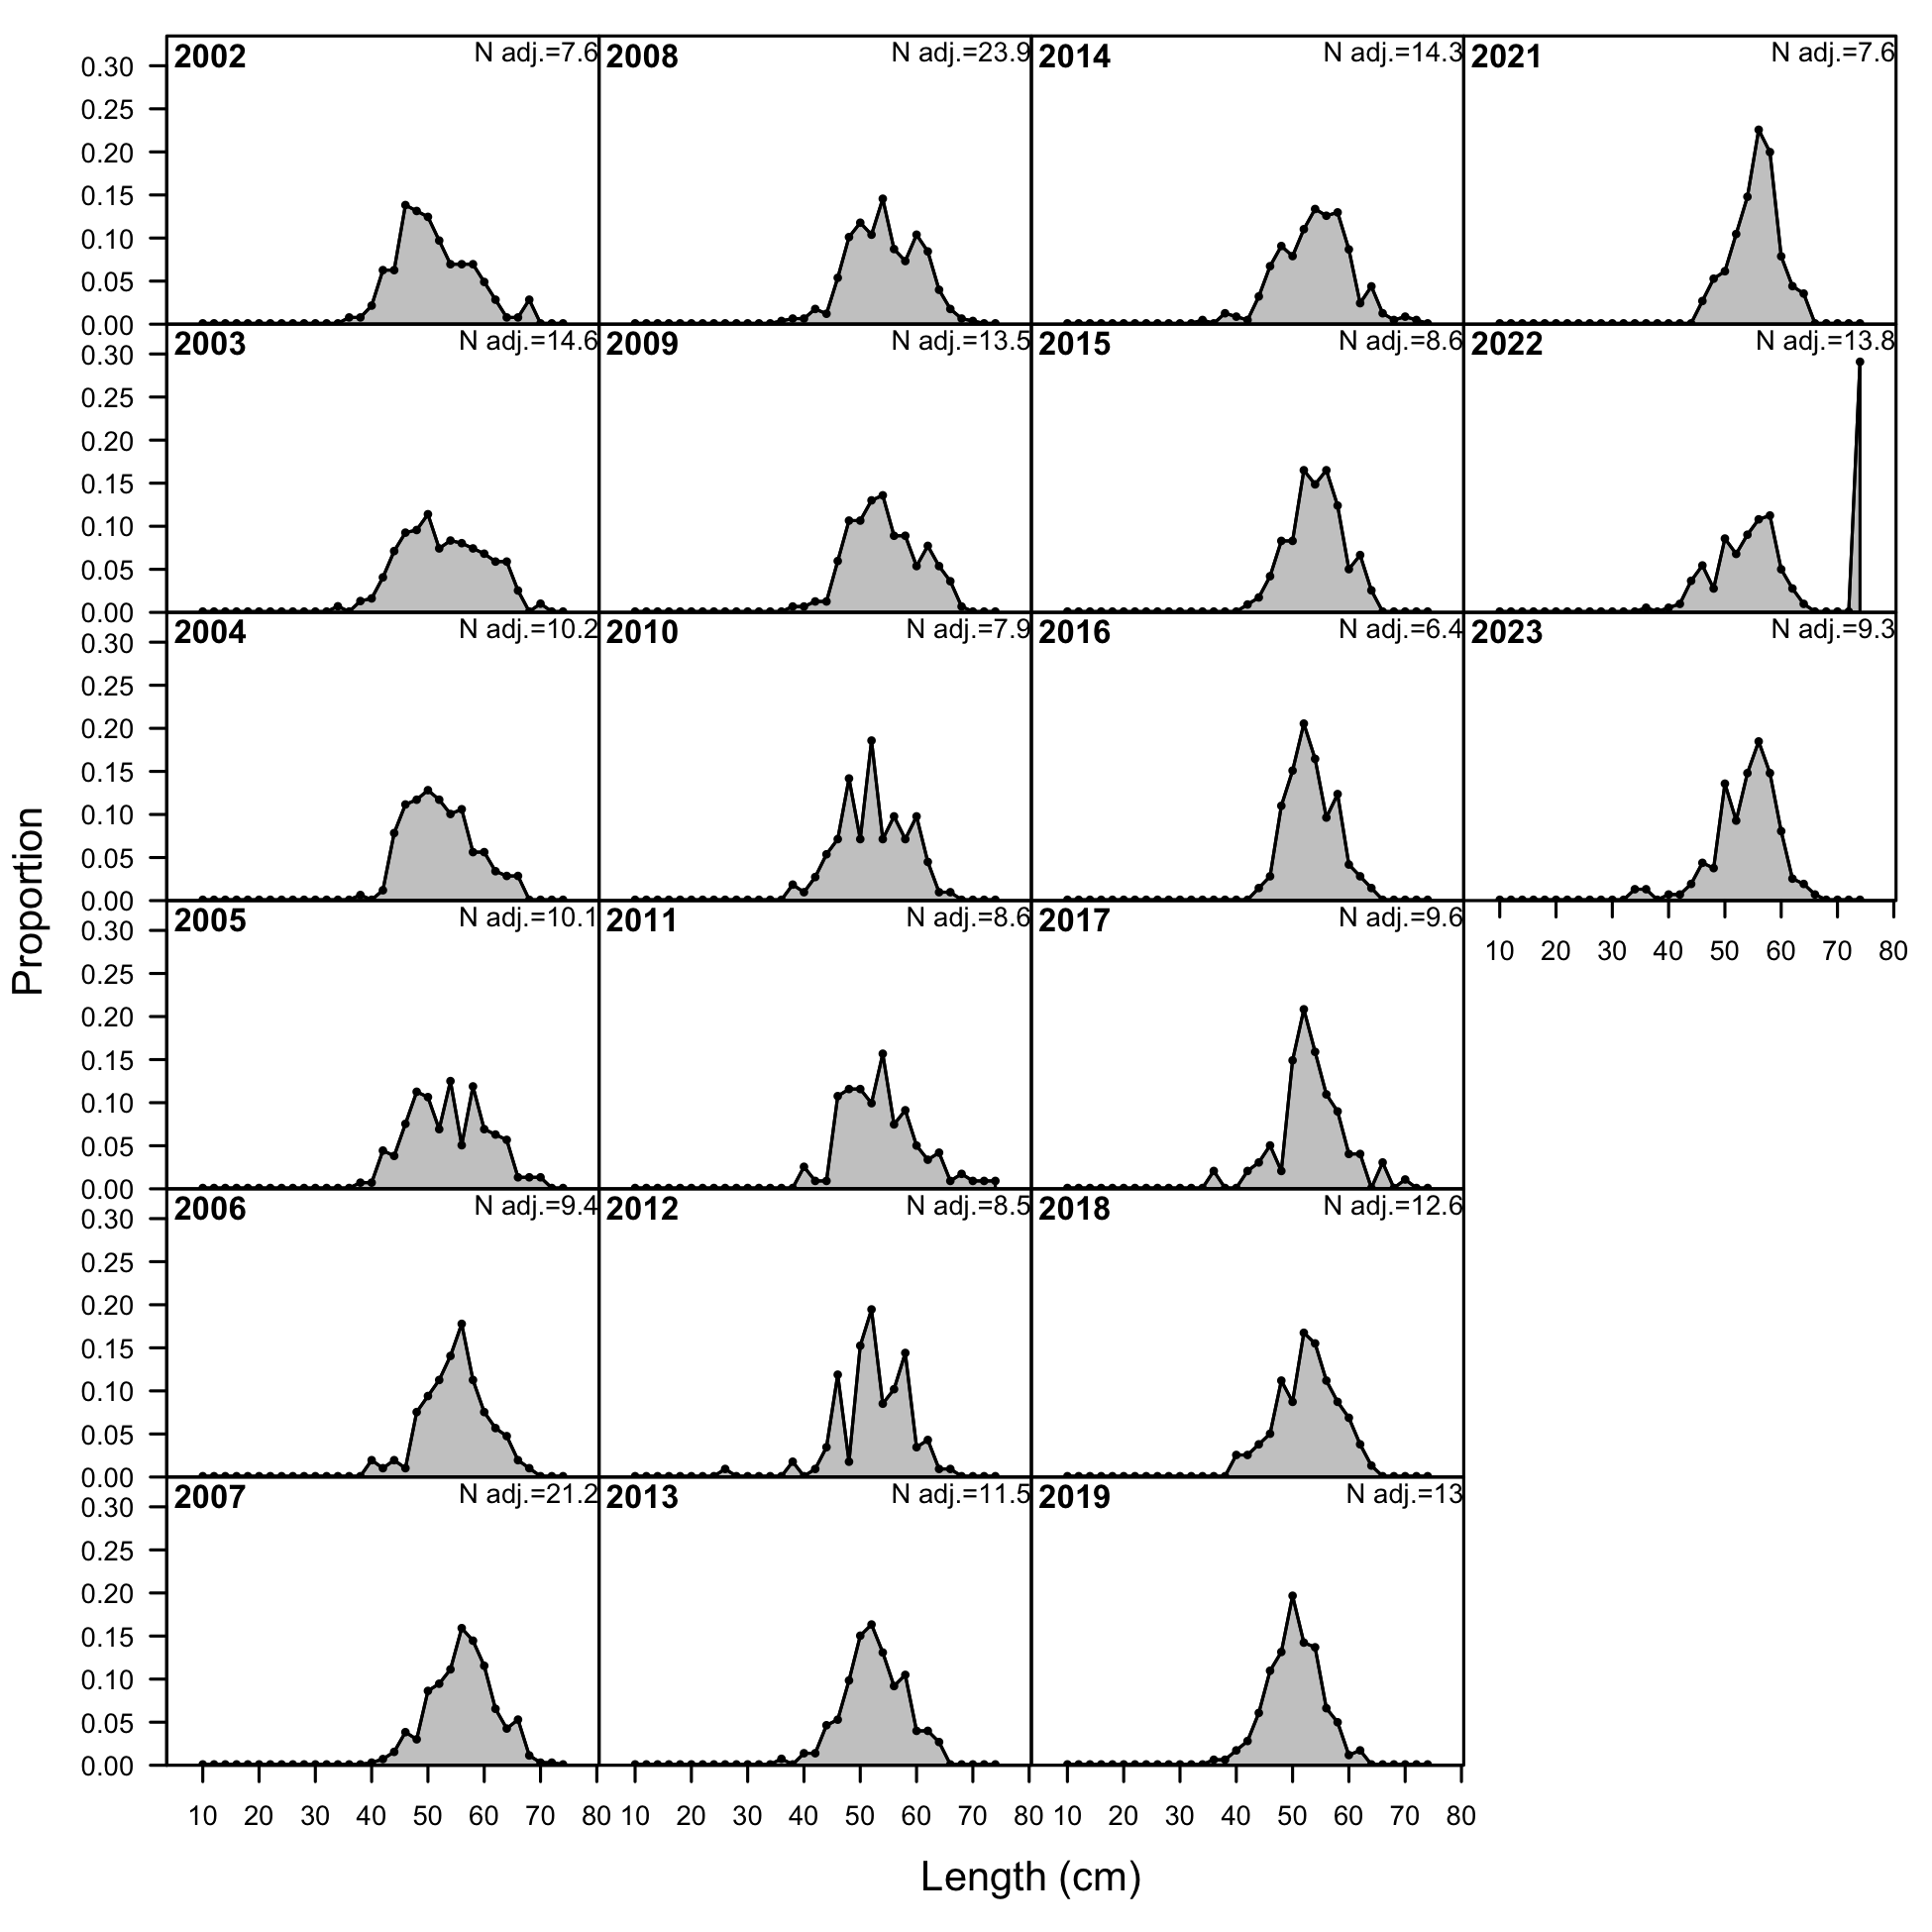
\includegraphics{figures/r4ss_plots/plots/comp_lendat_flt12mkt0.png}

}

\caption{\label{fig-IPHC_lencomps}Annual length composition data from
the IPHC longline survey.}

\end{figure}%

\clearpage

\begin{figure}

\centering{

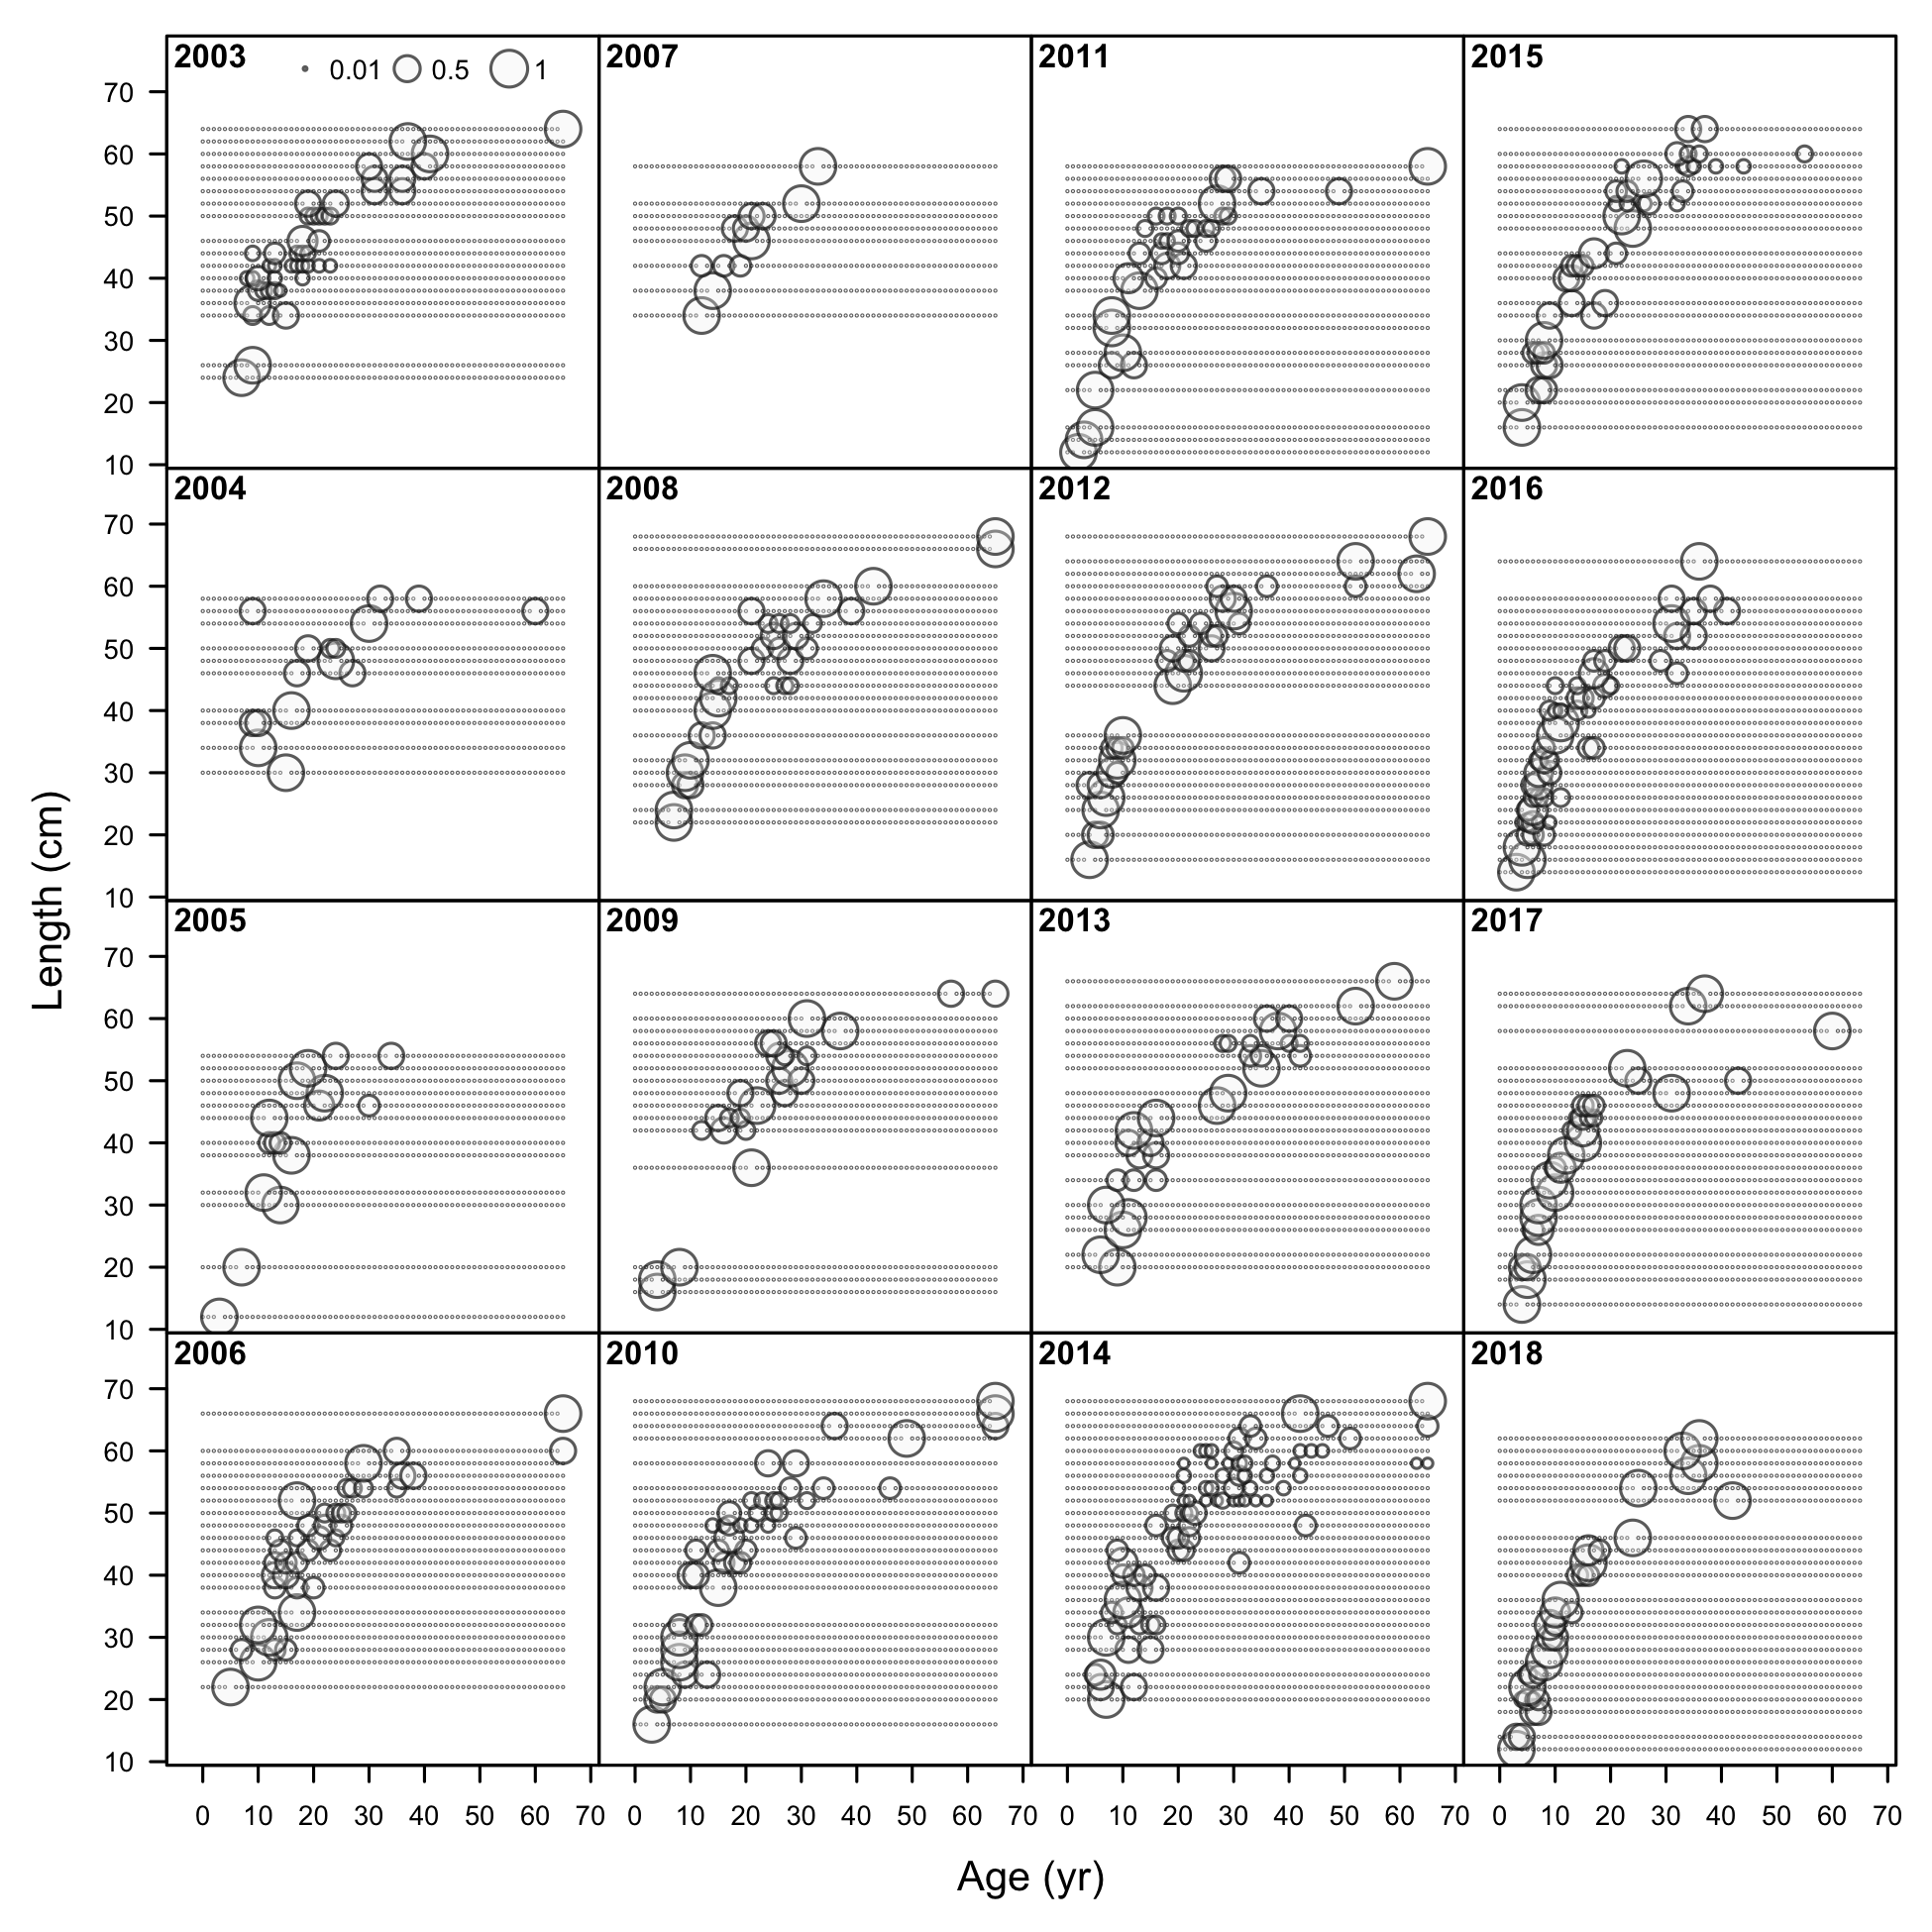
\includegraphics{figures/r4ss_plots/plots/comp_condAALdat_bubflt11mkt0_page1.png}

}

\caption{\label{fig-NWFSC_agecomps1}Annual unsexed conditional
age-at-length data for the WCBTS (1 of 2).}

\end{figure}%

\begin{figure}

\centering{

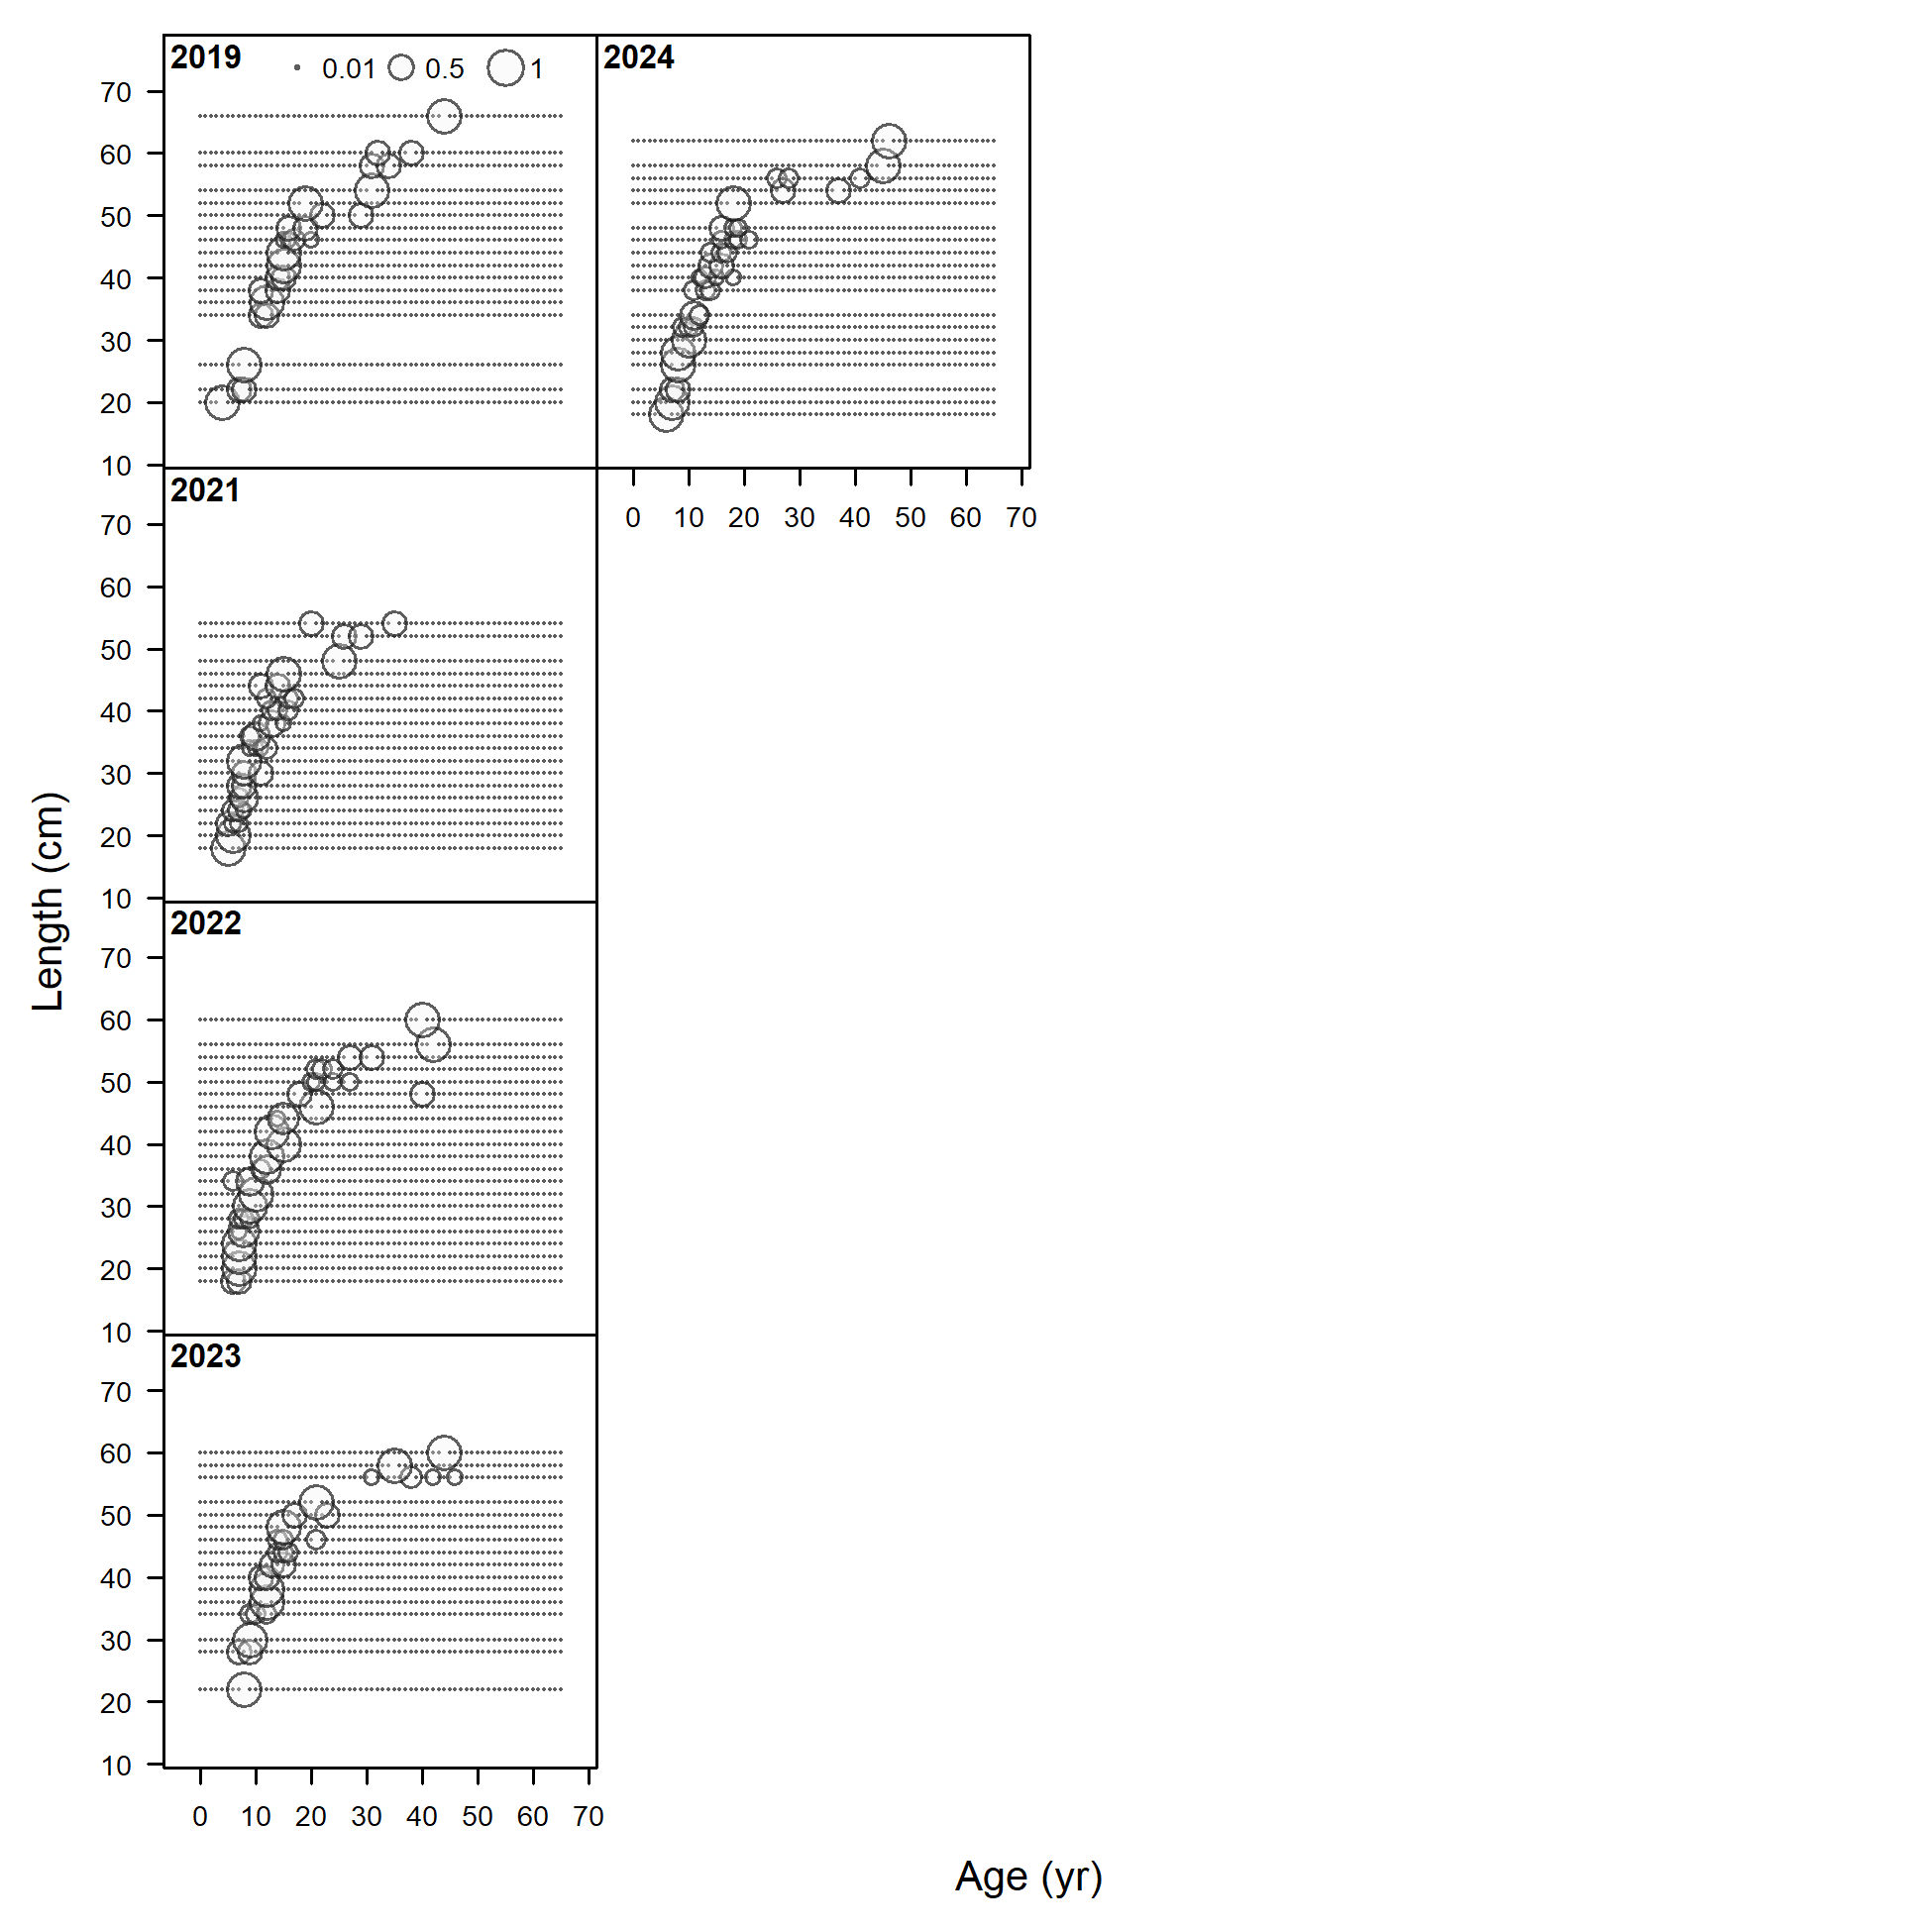
\includegraphics{figures/r4ss_plots/plots/comp_condAALdat_bubflt11mkt0_page2.png}

}

\caption{\label{fig-NWFSC_agecomps2}Annual unsexed conditional
age-at-length data for the WCBTS (2 of 2).}

\end{figure}%

\begin{figure}

\centering{

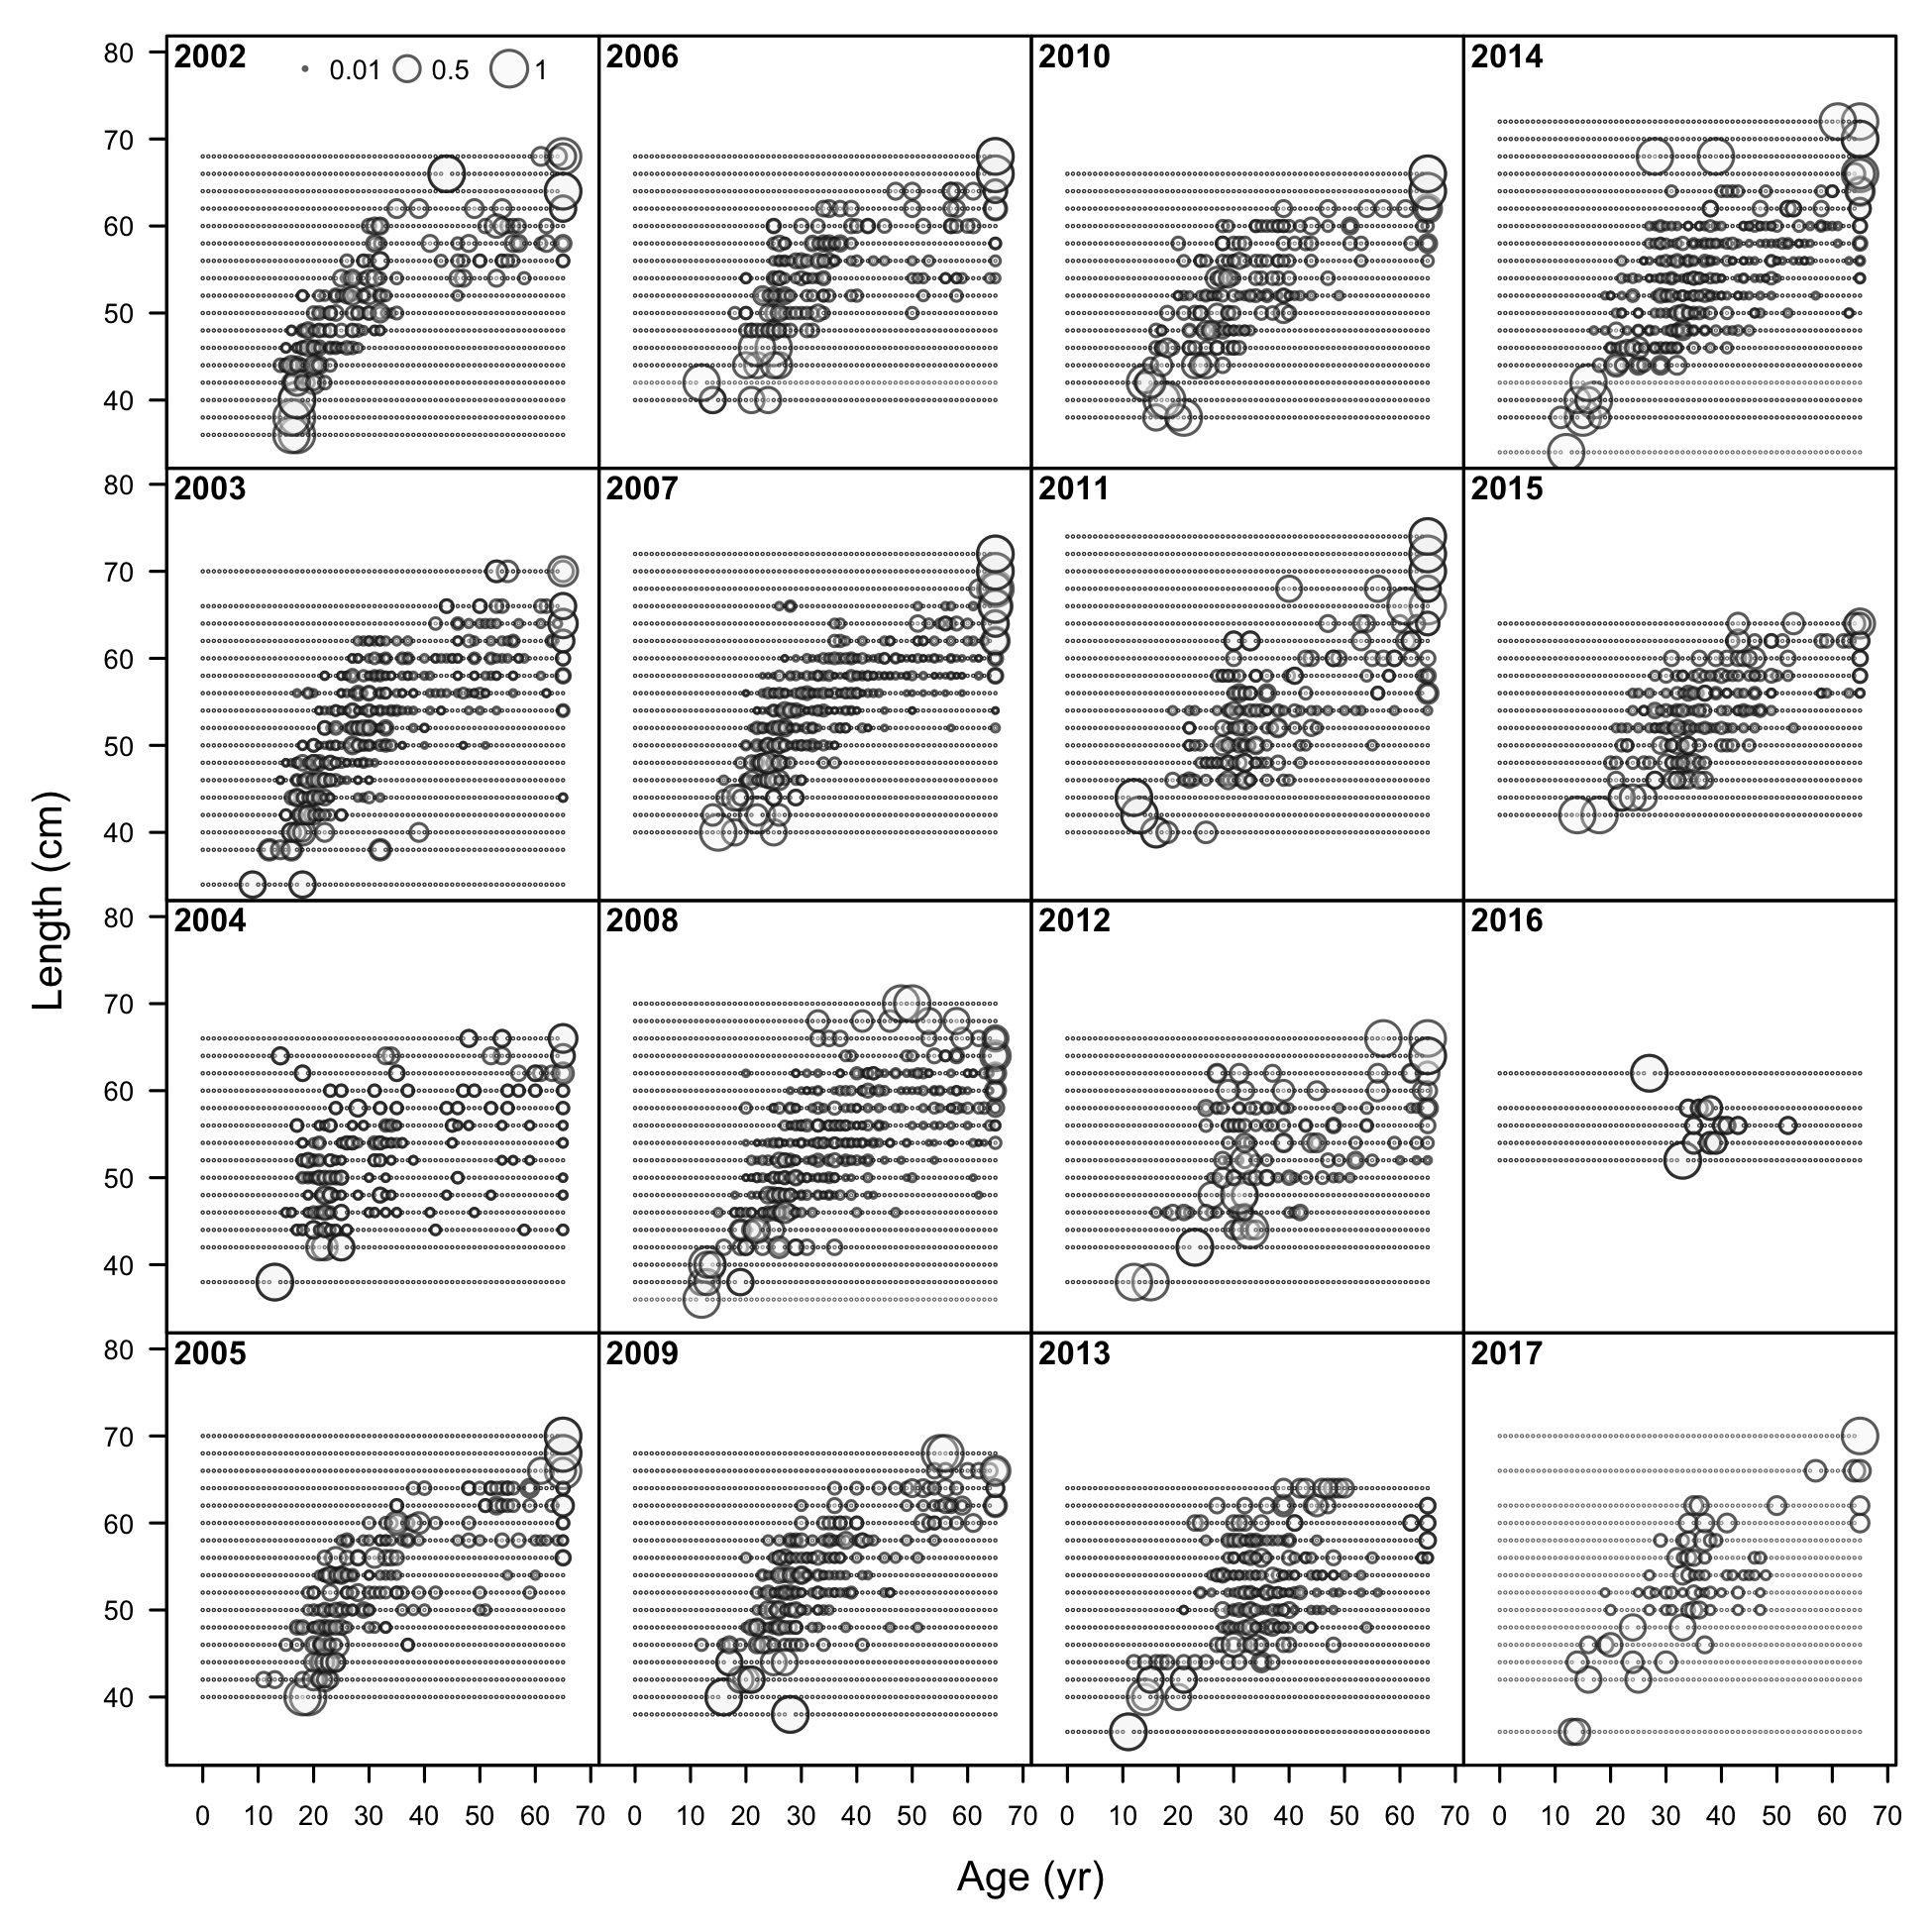
\includegraphics{figures/r4ss_plots/plots/comp_condAALdat_bubflt12mkt0_page1.png}

}

\caption{\label{fig-IPHC_agecomps1}Annual unsexed conditional
age-at-length data for the IPHC (1 of 2).}

\end{figure}%

\begin{figure}

\centering{

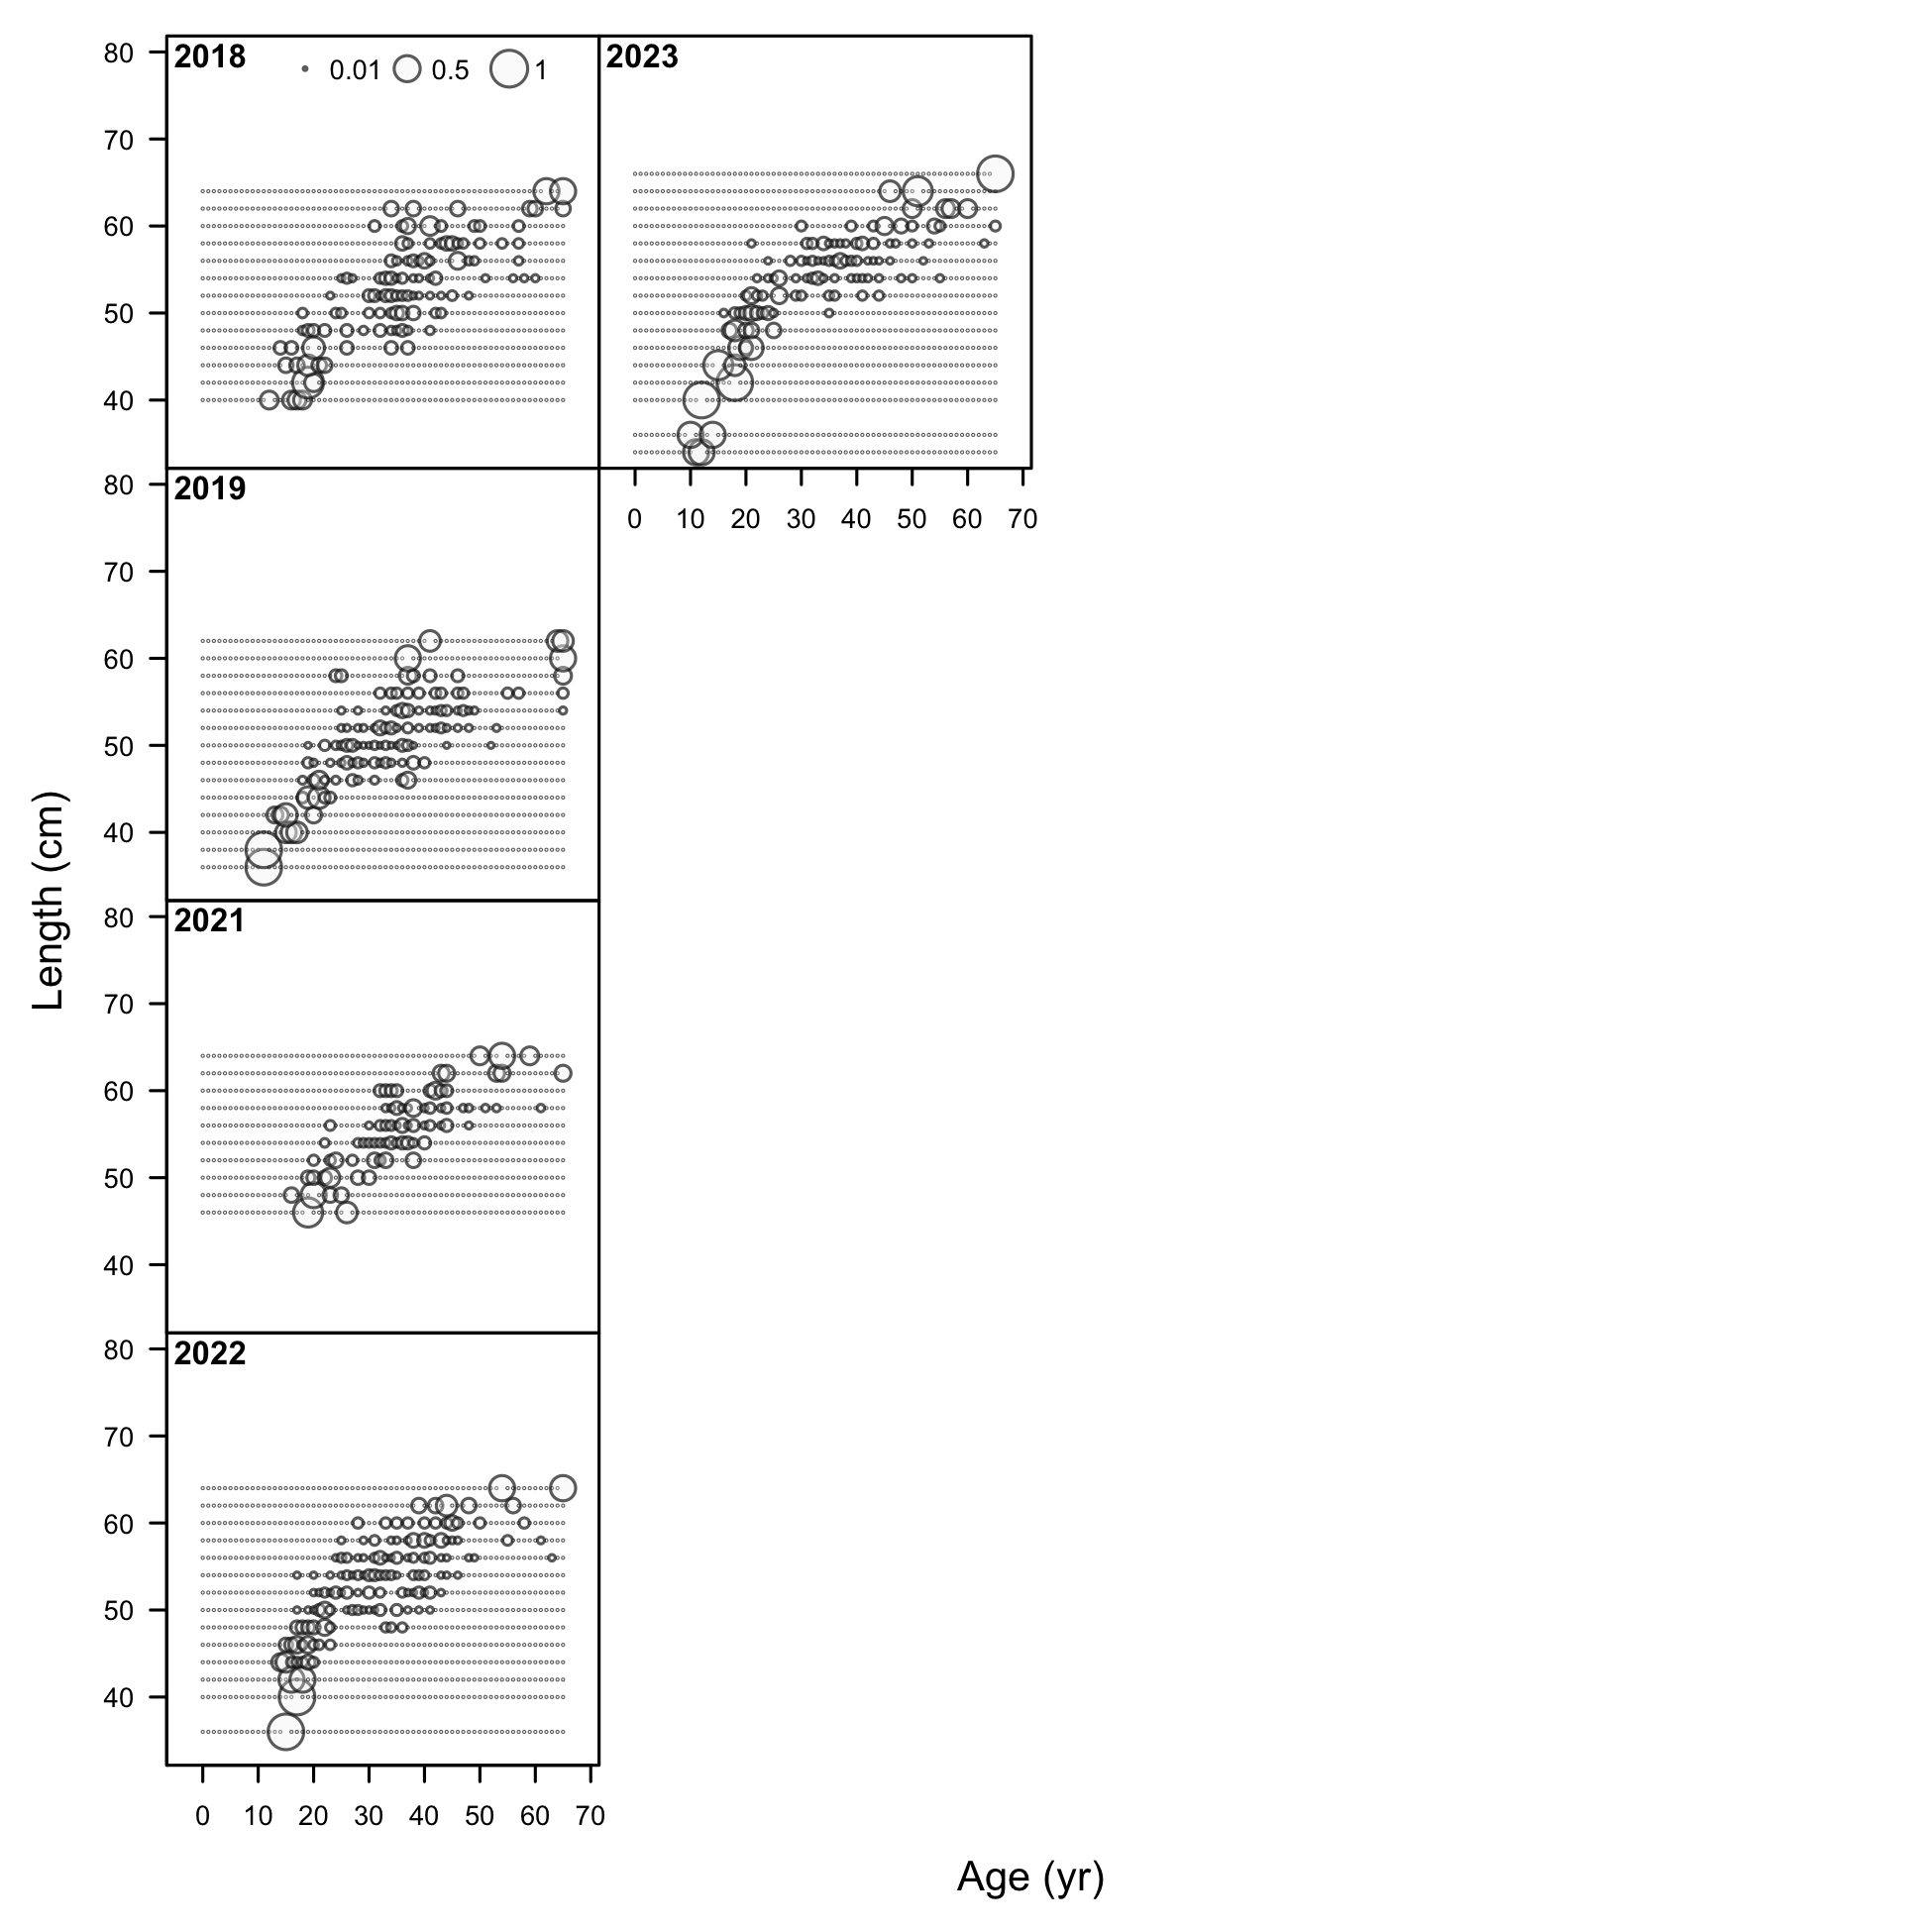
\includegraphics{figures/r4ss_plots/plots/comp_condAALdat_bubflt12mkt0_page2.png}

}

\caption{\label{fig-IPHC_agecomps2}Annual unsexed conditional
age-at-length data for the IPHC (1 of 2).}

\end{figure}%

\begin{figure}

\centering{

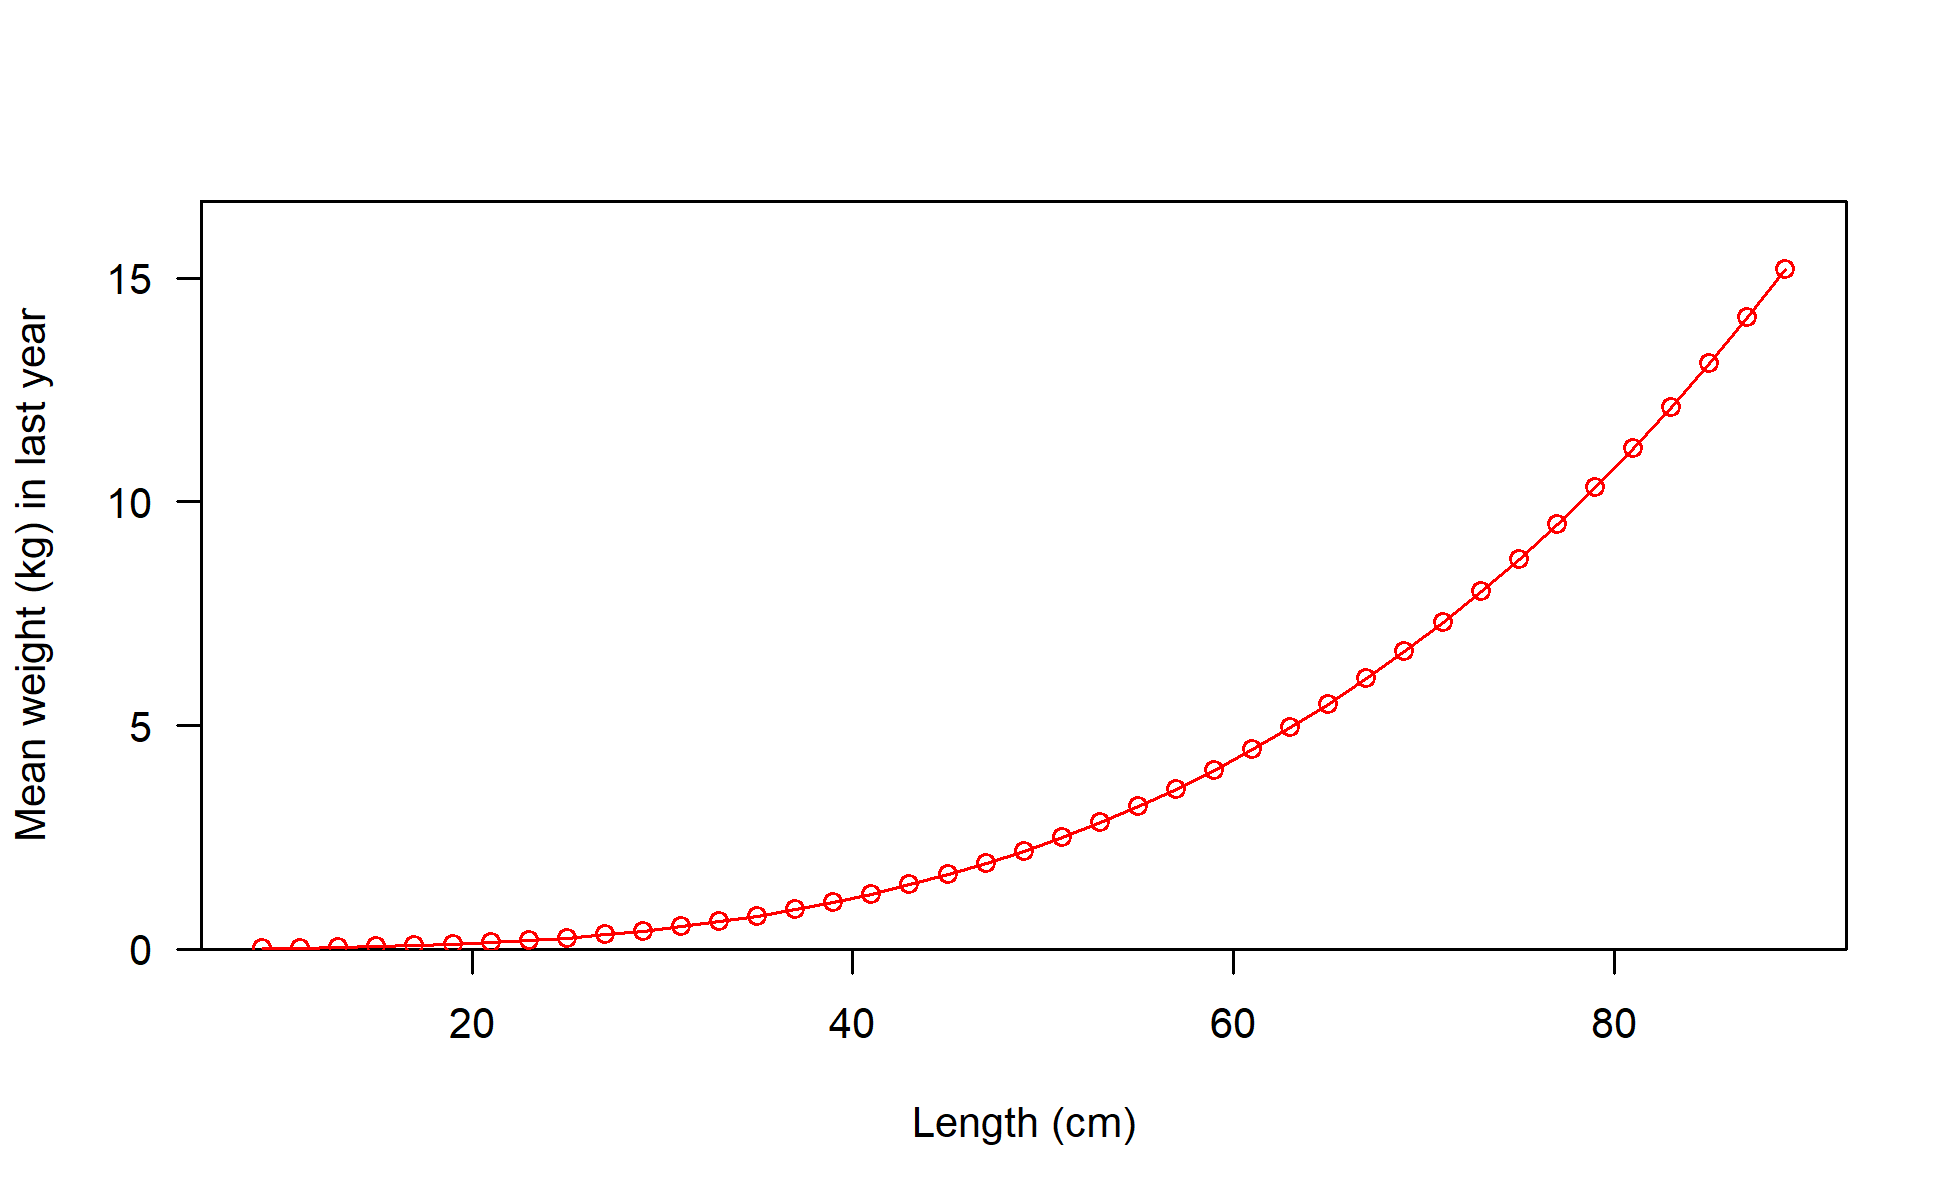
\includegraphics{figures/r4ss_plots/plots/bio5_weightatsize.png}

}

\caption{\label{fig-LWrel}Updated weight-at-length relationship.}

\end{figure}%

\begin{figure}

\centering{

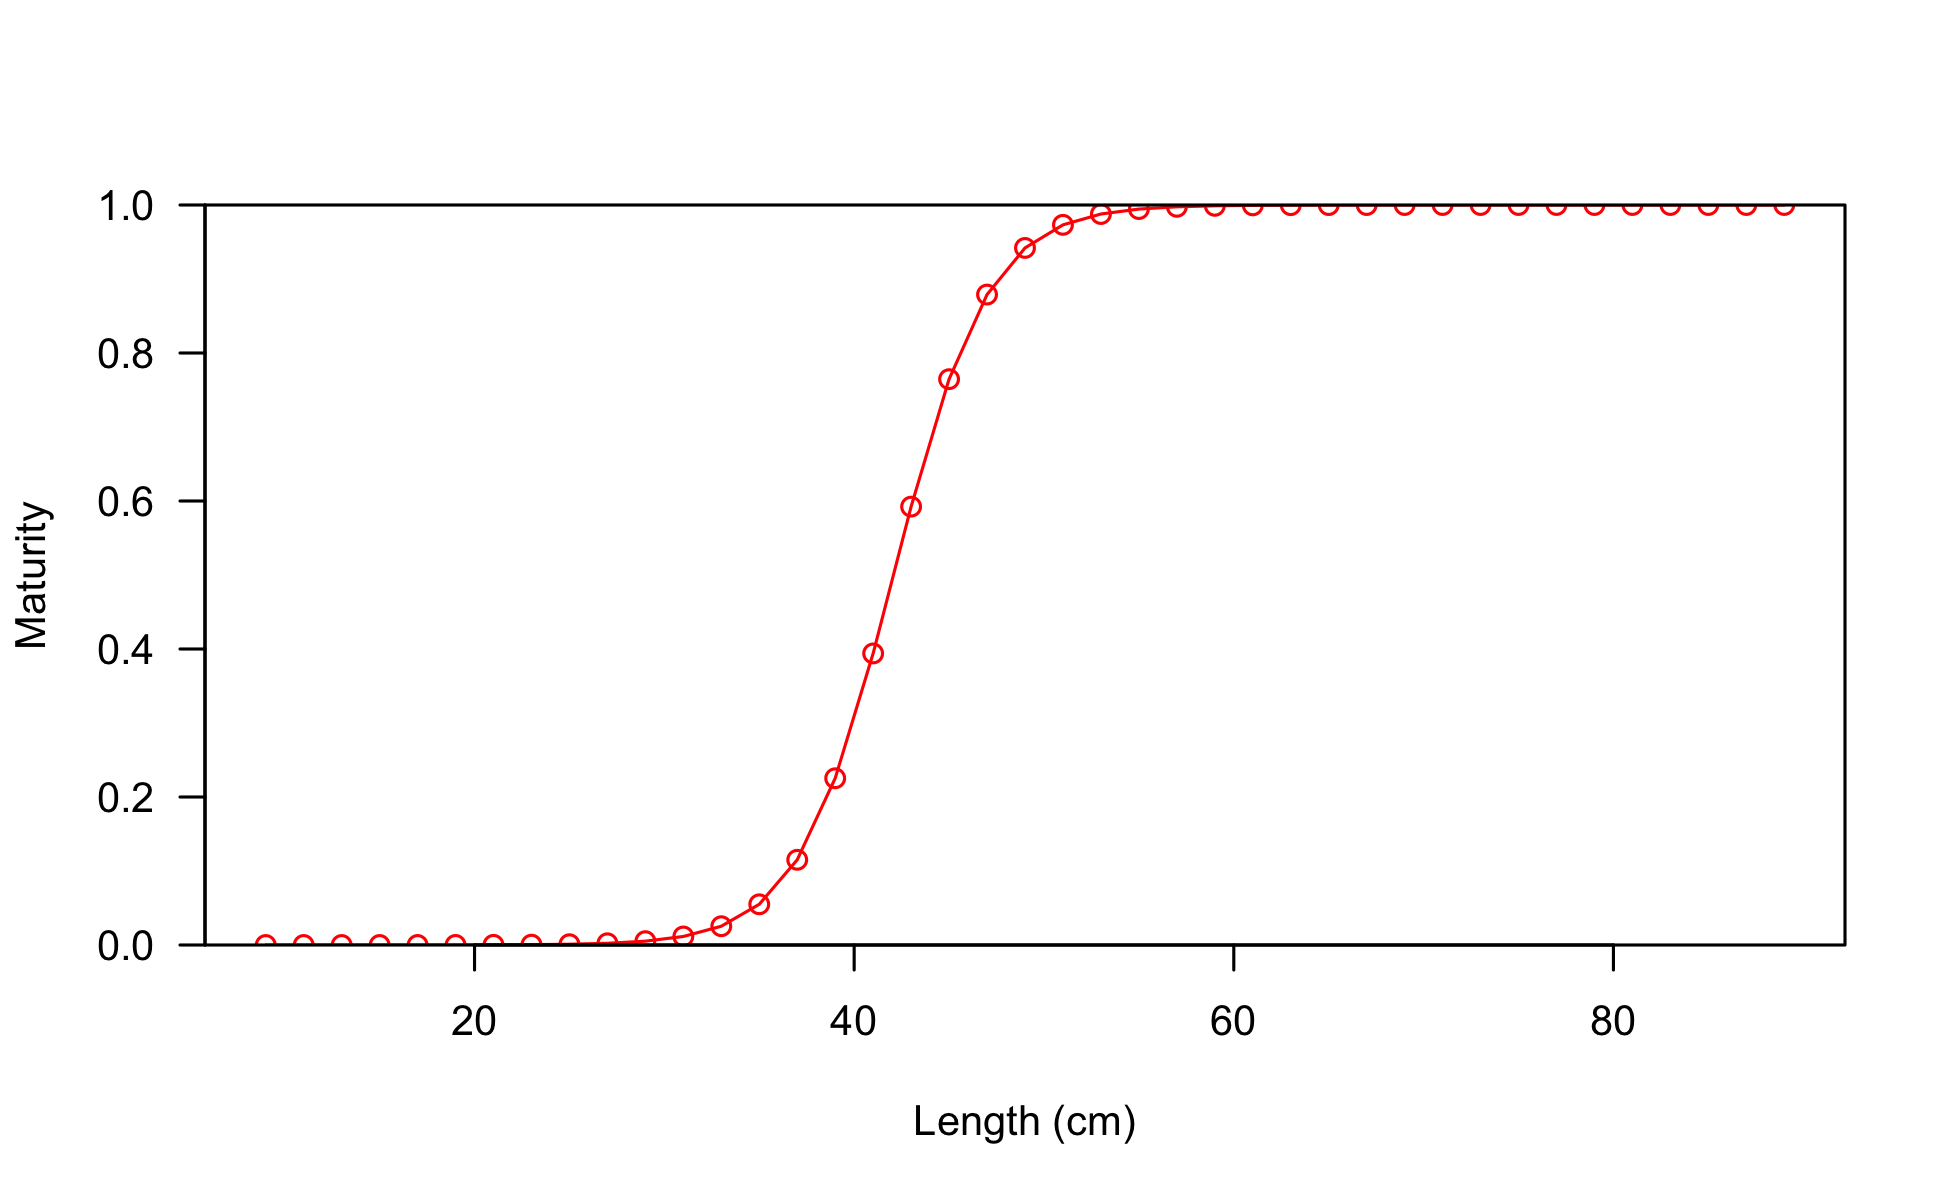
\includegraphics{figures/r4ss_plots/plots/bio6_maturity.png}

}

\caption{\label{fig-maturity}Maturity at length relationship used in the
base model for Yelloweye Rockfish.}

\end{figure}%

\begin{figure}

\centering{

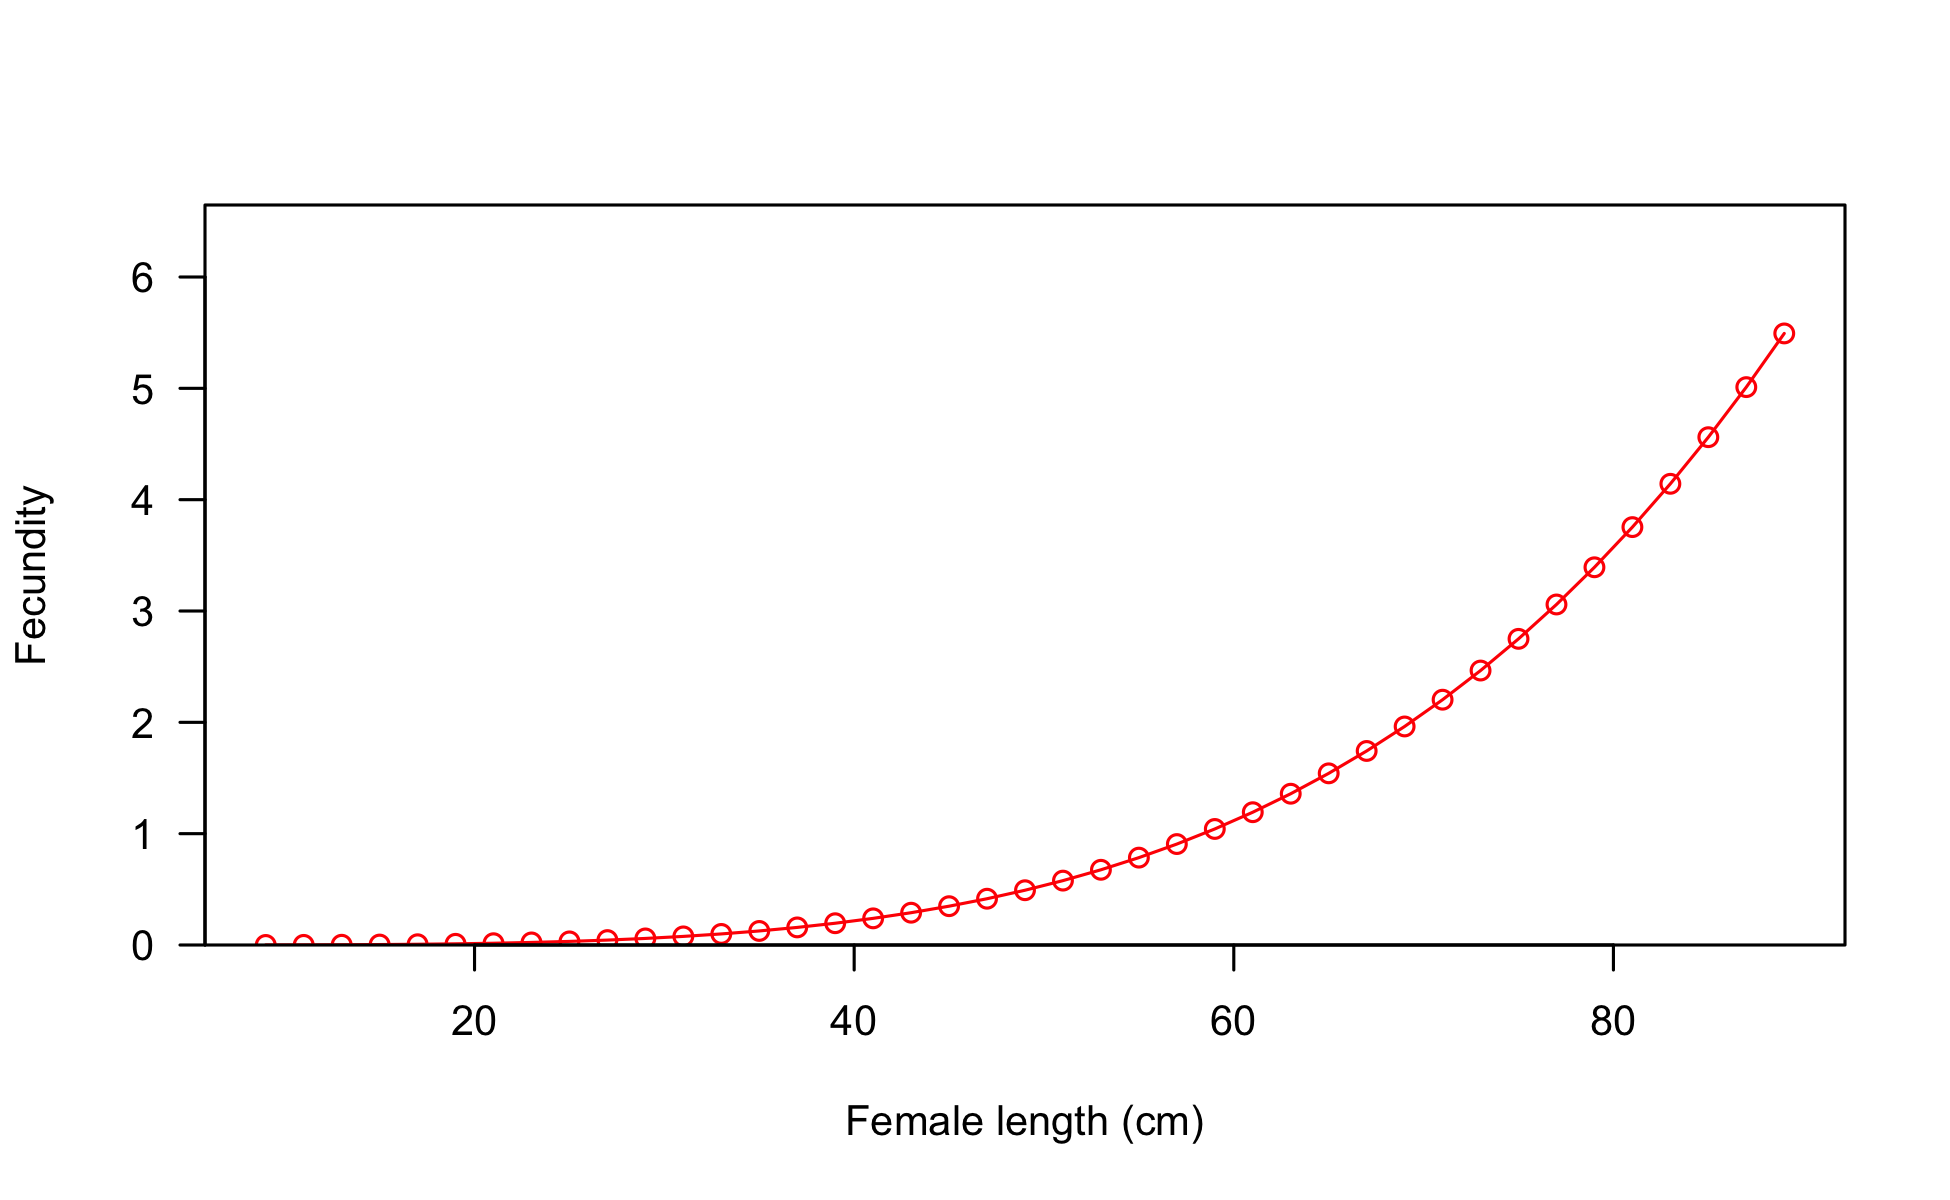
\includegraphics{figures/r4ss_plots/plots/bio9_fecundity_len.png}

}

\caption{\label{fig-fecundity}Fecundity at length relationship used in
the base model for Yelloweye Rockfish.}

\end{figure}%

\begin{figure}

\centering{

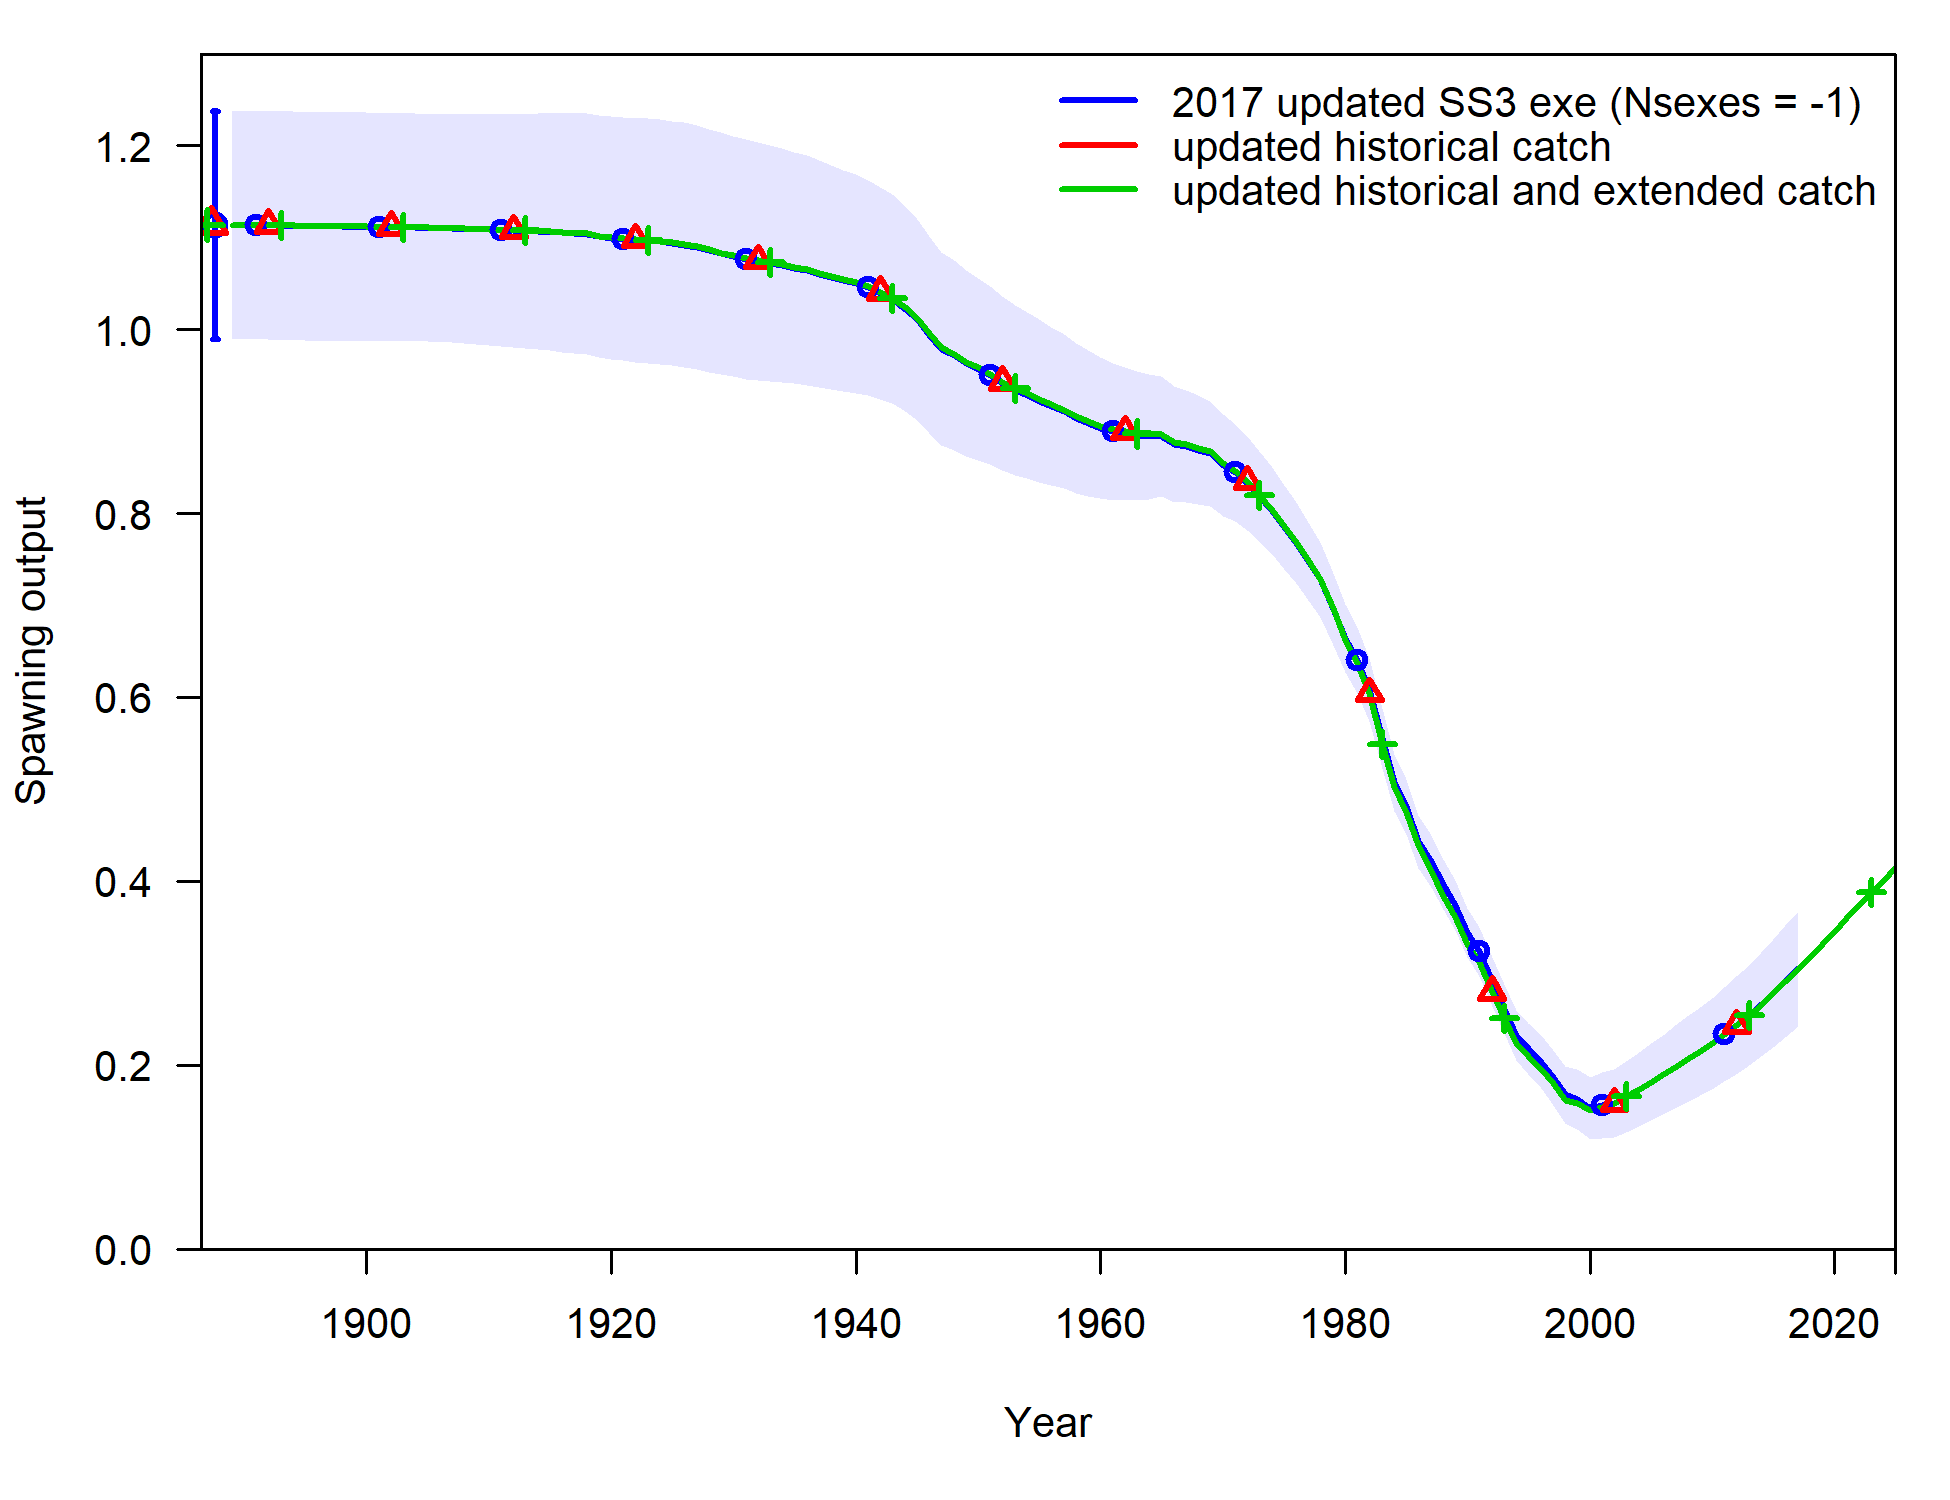
\includegraphics{figures/bridging/3_extendedcatch/compare2_spawnbio_uncertainty.png}

}

\caption{\label{fig-bridge3-comp2}Comparison of the spawning output
(millions of eggs) of the 2017 model with an updated SS3 executable
(blue), updated historical catch data (red), and catch extened to 2024
(green).}

\end{figure}%

\begin{figure}

\centering{

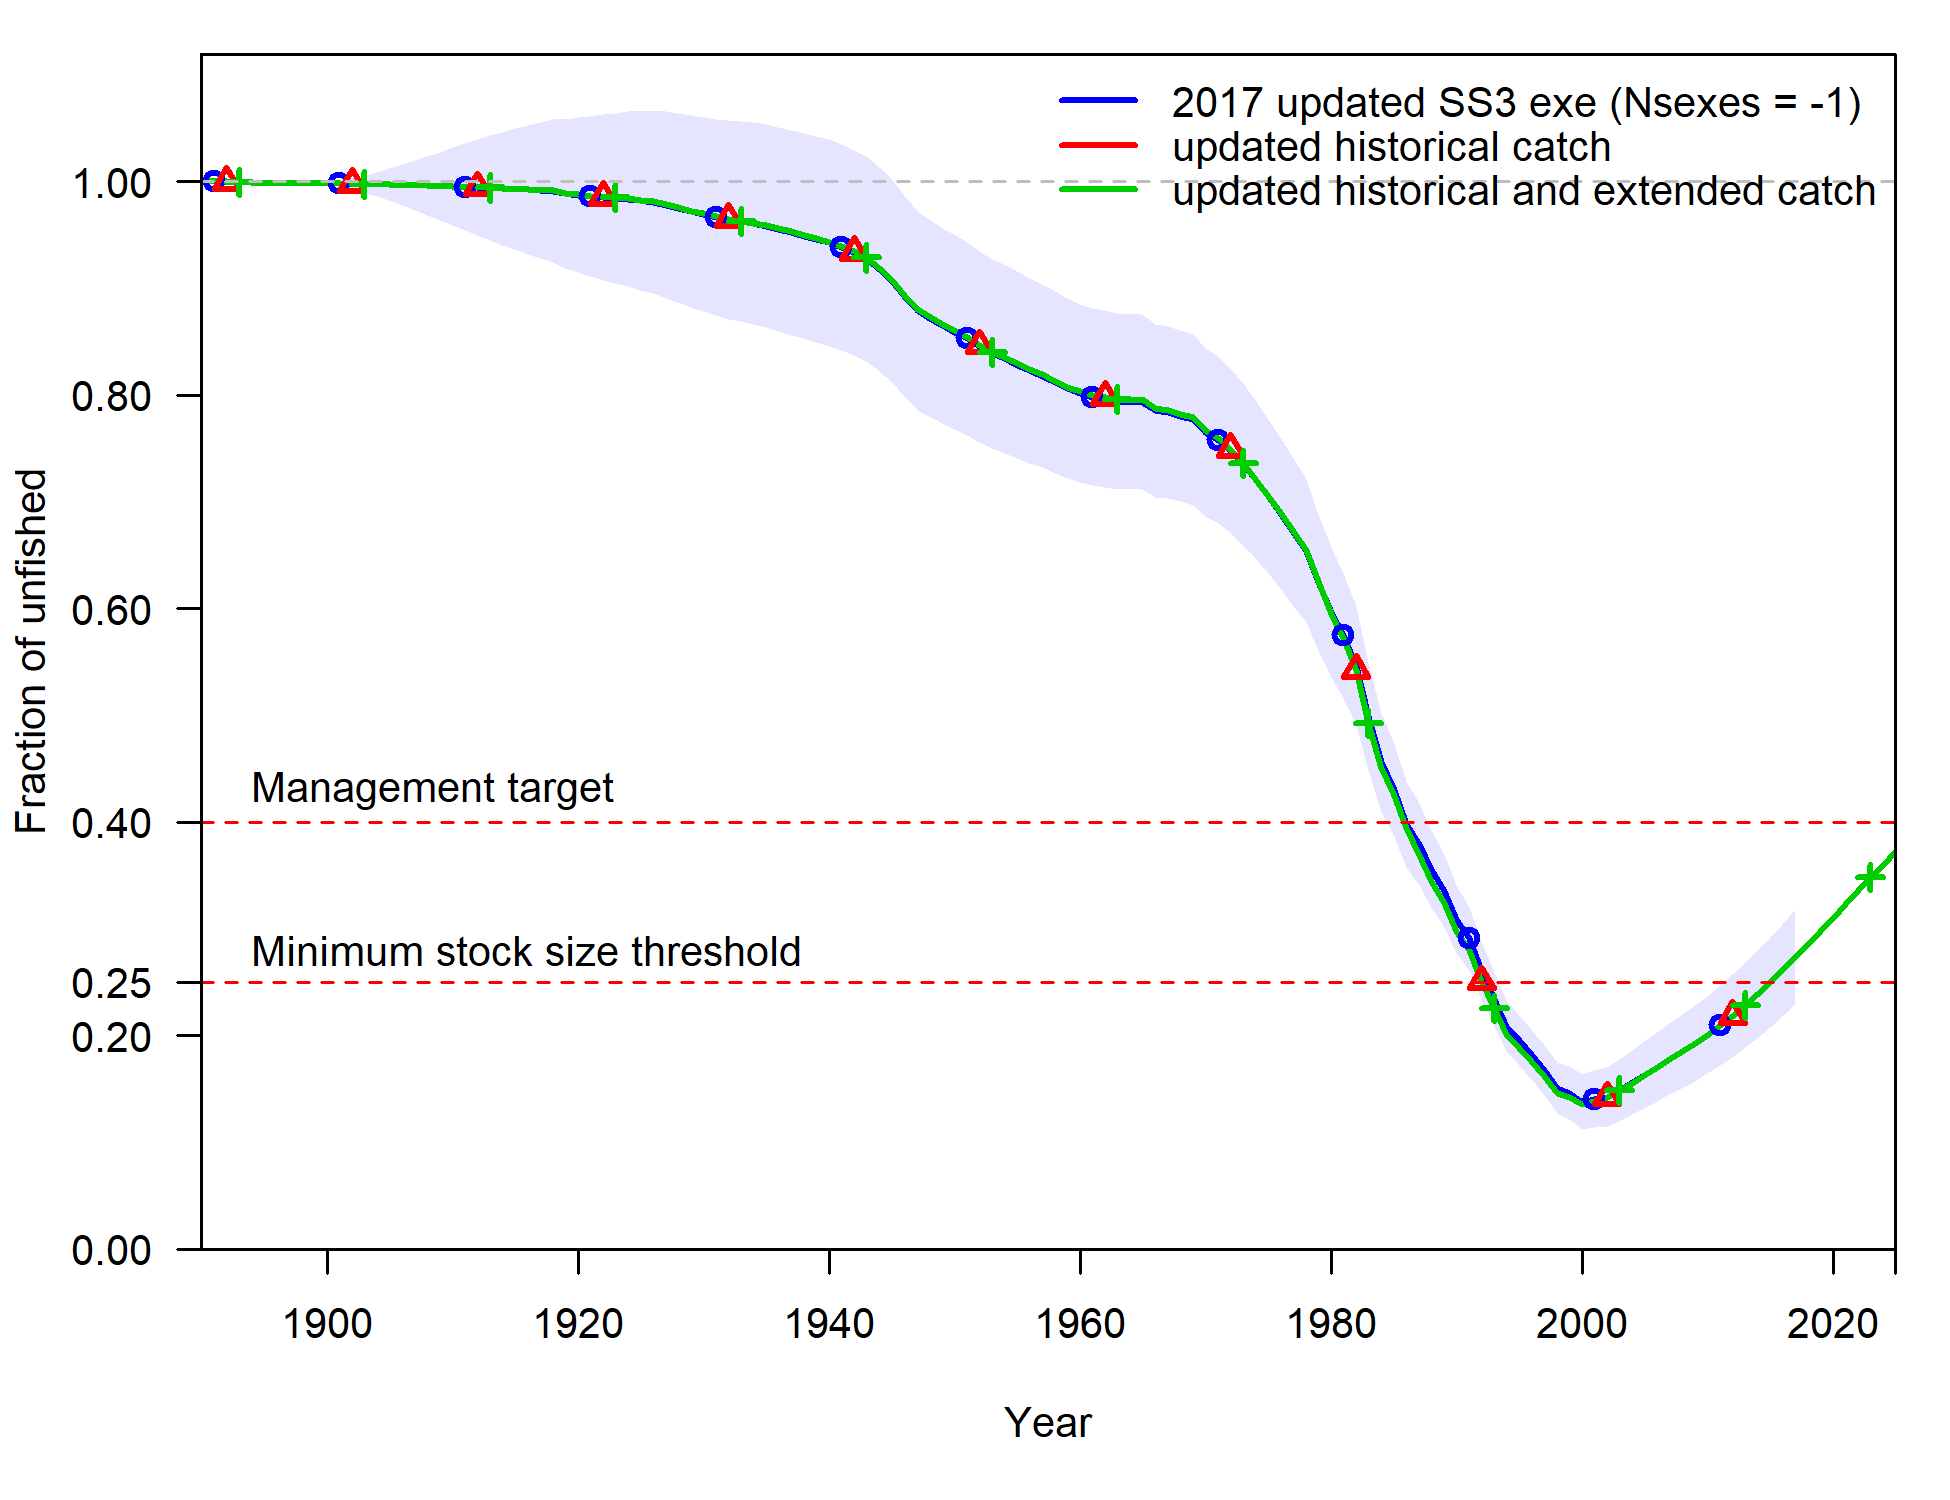
\includegraphics{figures/bridging/3_extendedcatch/compare4_Bratio_uncertainty.png}

}

\caption{\label{fig-bridge3-comp4}Comparison of the stock status of the
2017 model with an updated SS3 executable (blue), updated historical
catch data (red), and catch extened to 2024 (green) relative to the
management target and minimum stock size threshold.}

\end{figure}%

\begin{figure}

\centering{

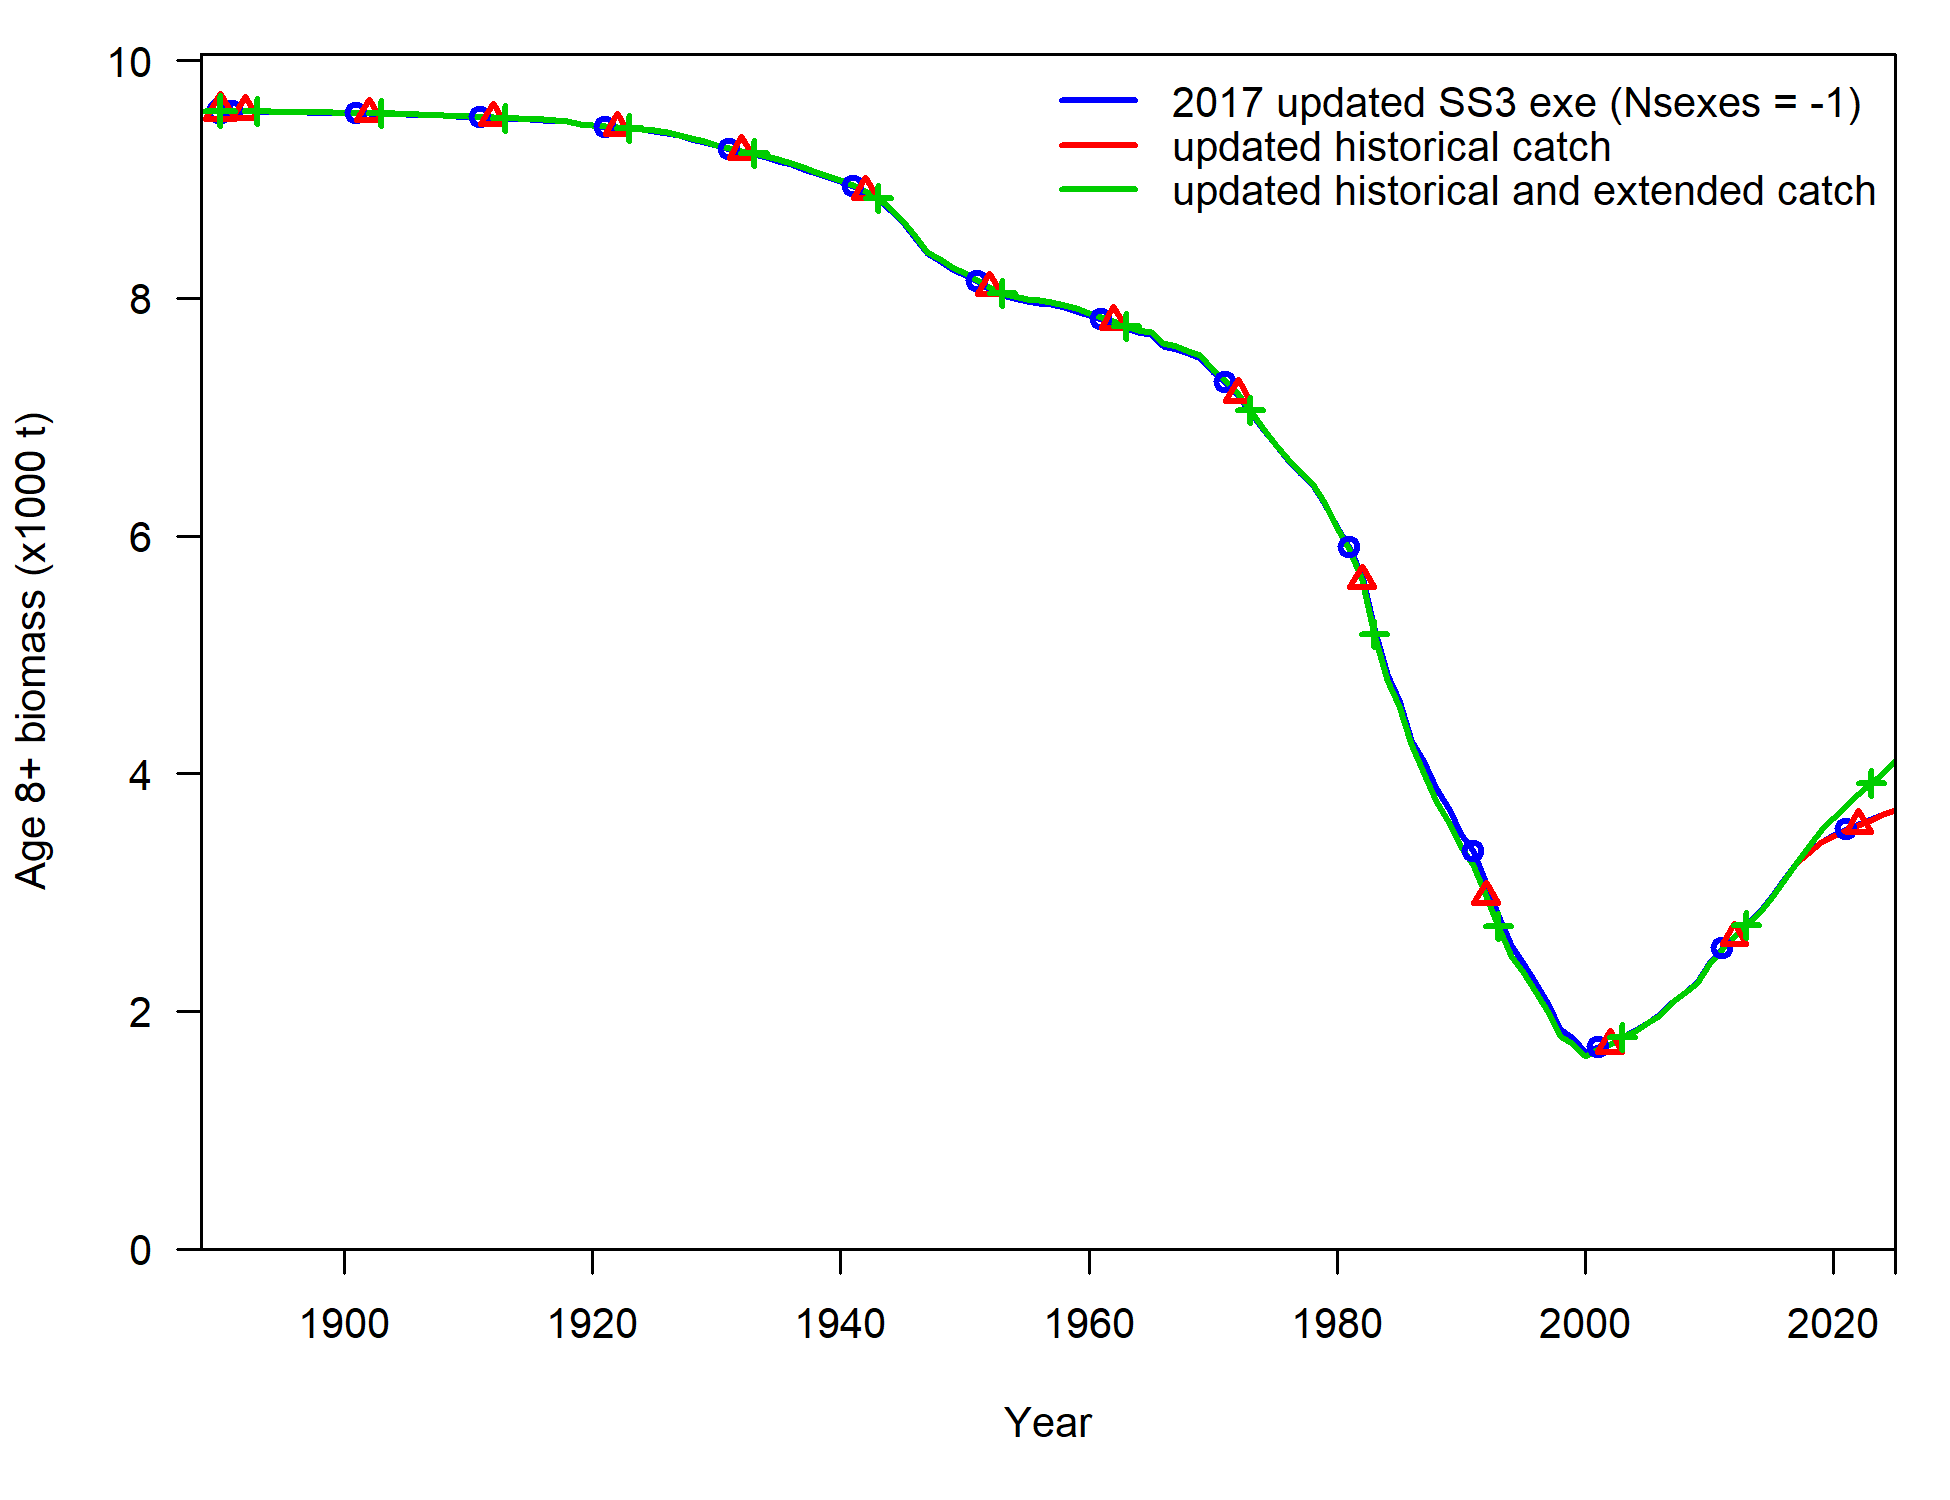
\includegraphics{figures/bridging/3_extendedcatch/compare18_smrybio.png}

}

\caption{\label{fig-bridge3-comp18}Comparison of adult Yelloweye
Rockfish biomass of the 2017 model with an updated SS3 executable
(blue), updated historical catch data (red), and catch extened to 2024
(green).}

\end{figure}%

\begin{figure}

\centering{

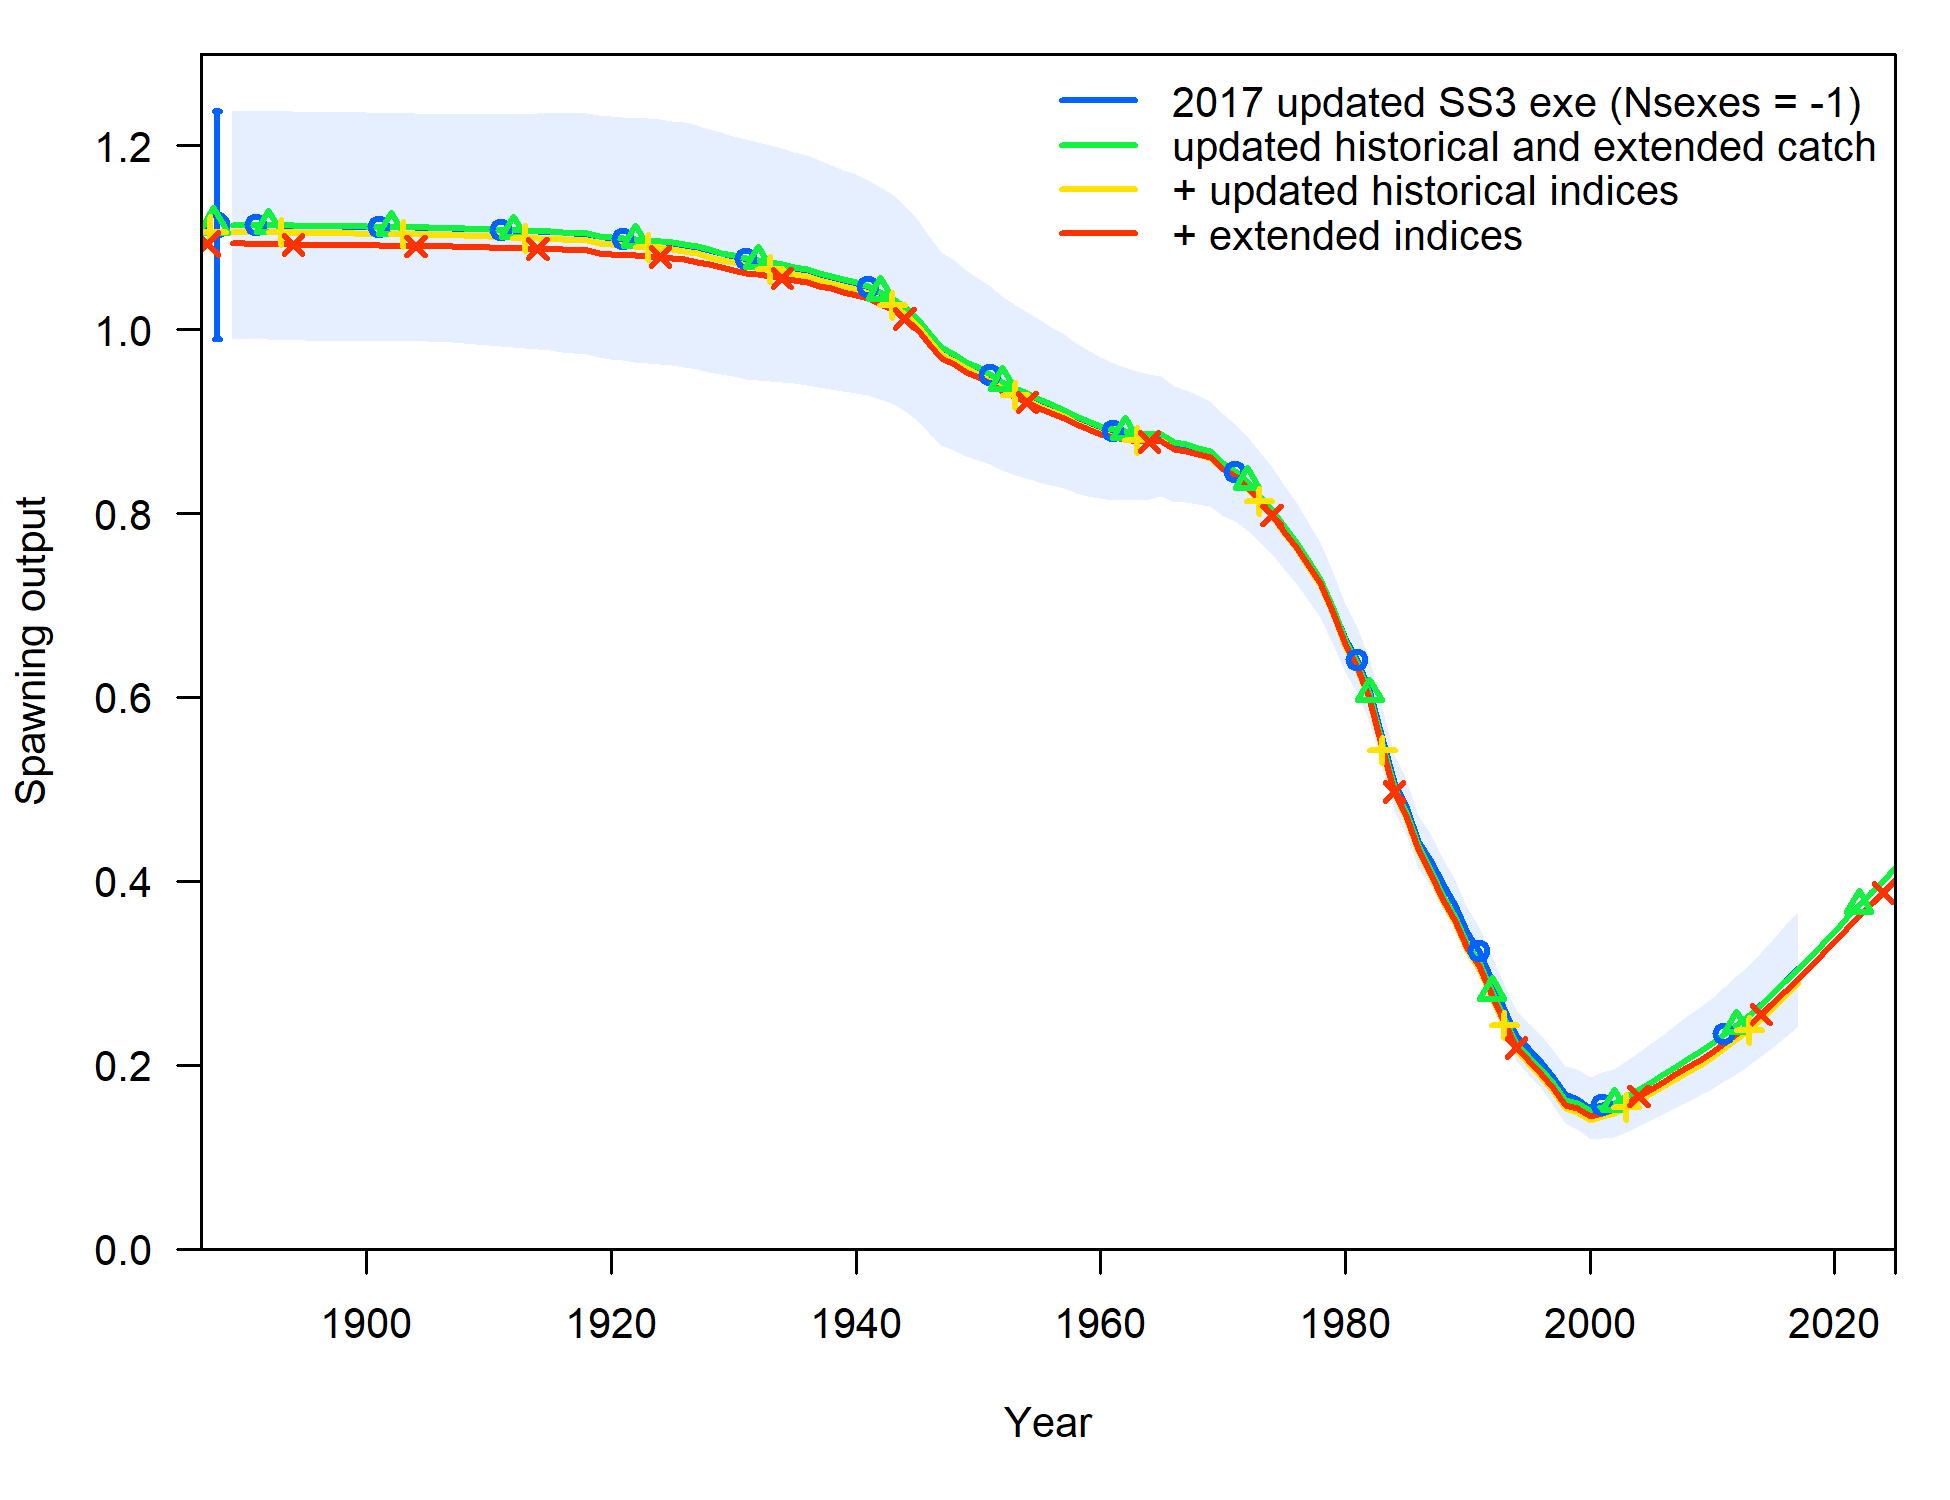
\includegraphics{figures/bridging/5_newindices/compare2_spawnbio_uncertainty.png}

}

\caption{\label{fig-bridge5-comp2}Comparison of the spawning output
(millions of eggs) of the 2017 model with an updated SS3 executable
(blue), updated and extended historical catch data (green), updated
historical indices (yellow), and indices extended to 2024 (red).}

\end{figure}%

\begin{figure}

\centering{

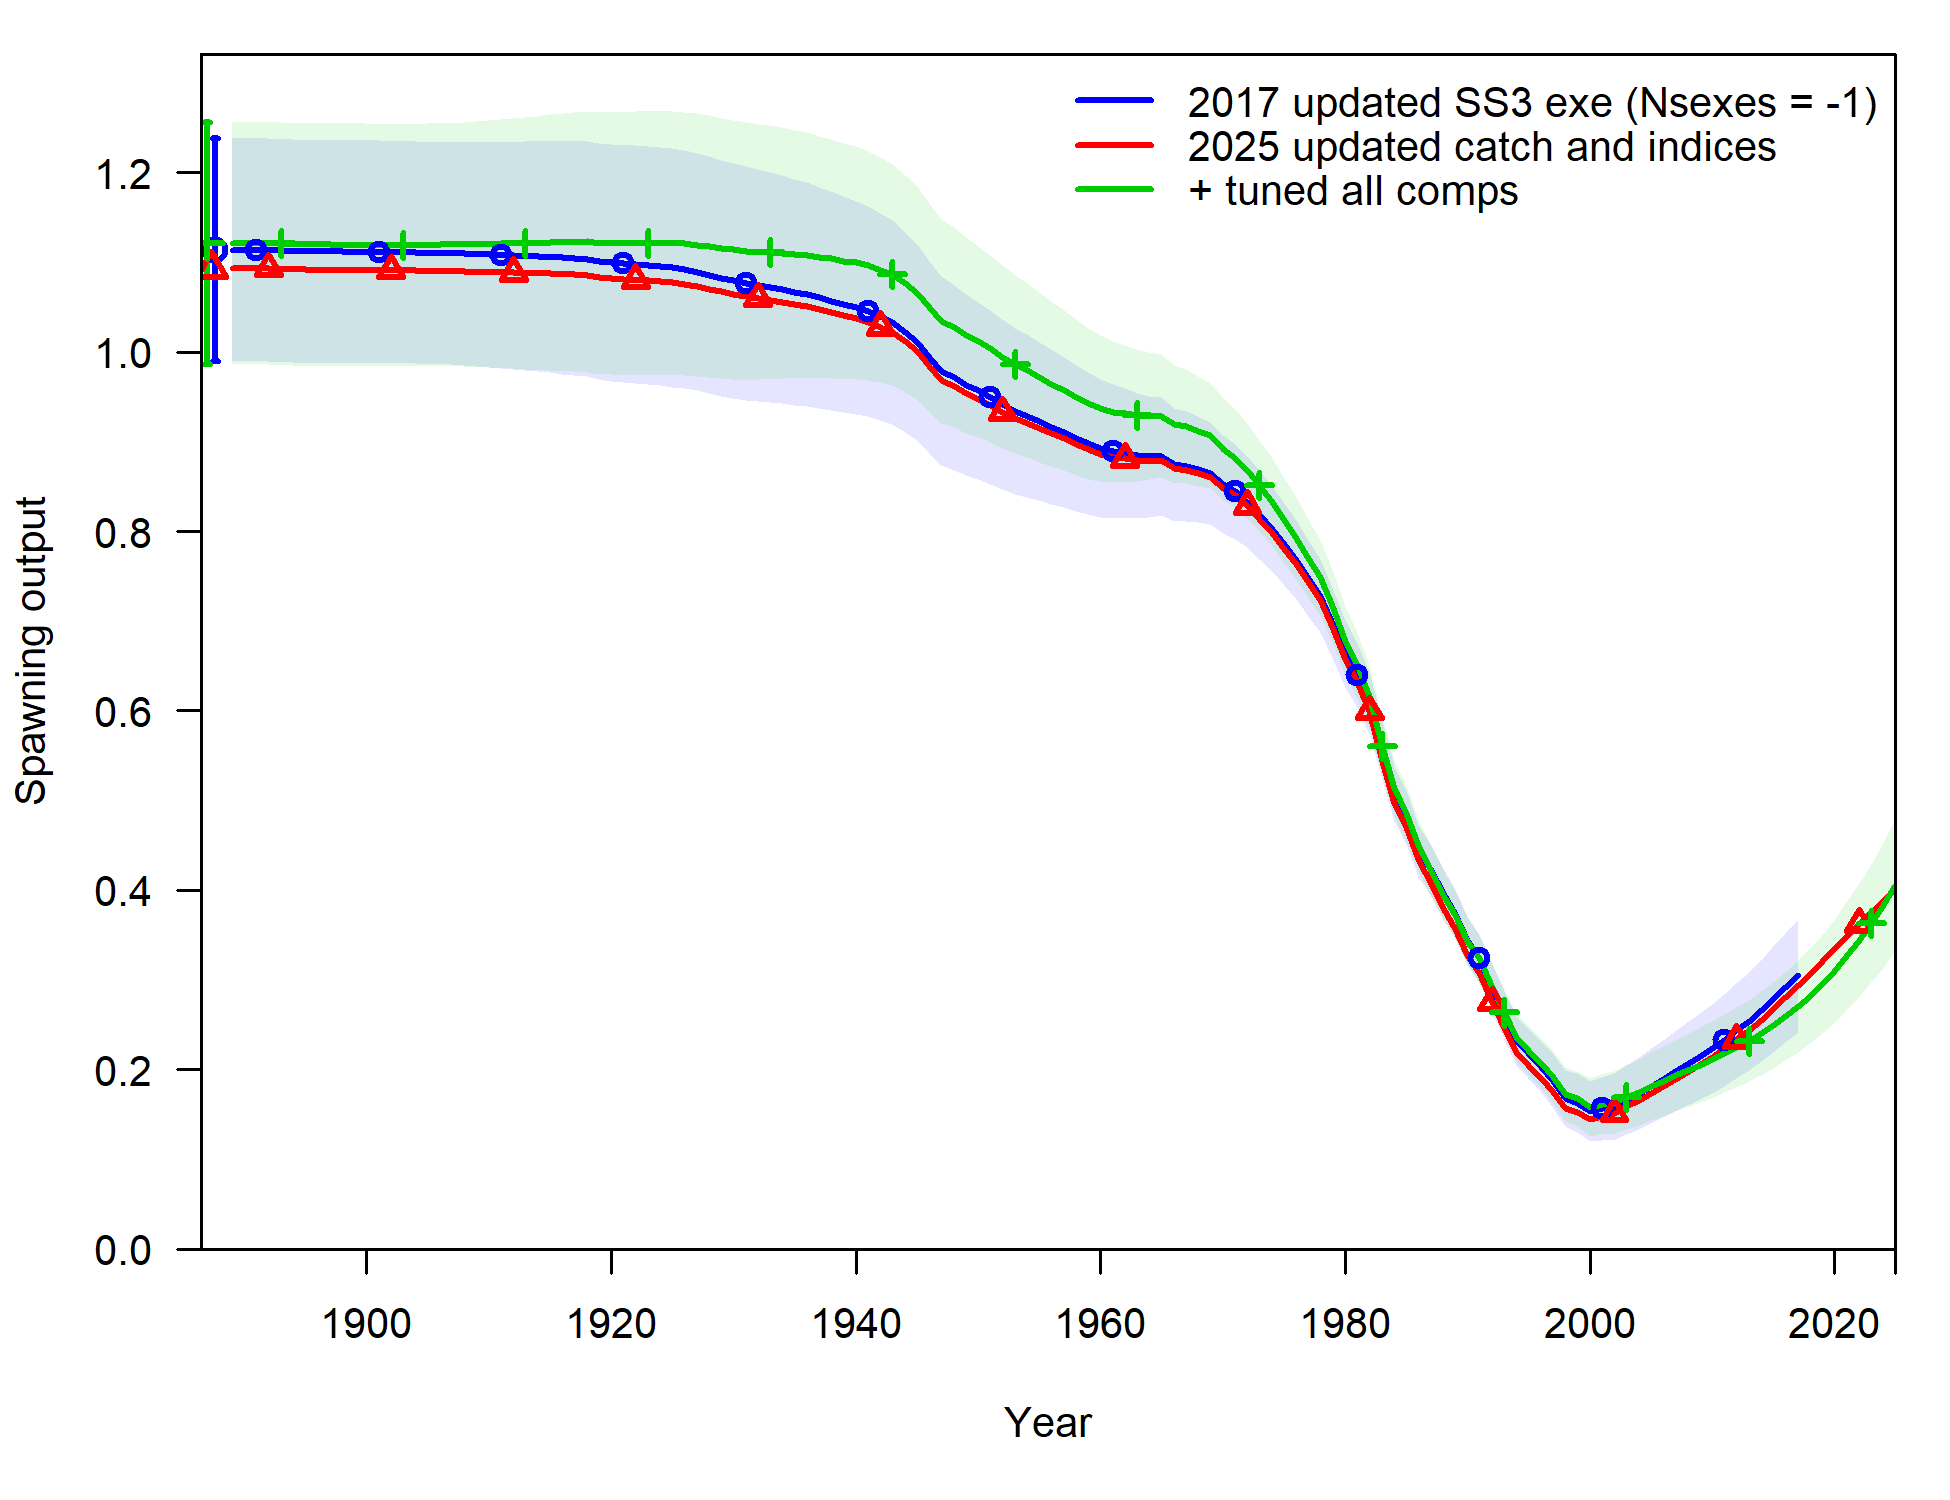
\includegraphics{figures/bridging/14_tunecomps/compare2_spawnbio_uncertainty.png}

}

\caption{\label{fig-bridge14-comp2}Comparison of the spawning output
(millions of eggs) of the 2017 model with an updated SS3 executable
(blue), updated and extended catch and indices (red), and all tuned
length and age composition data (green).}

\end{figure}%

\begin{figure}

\centering{

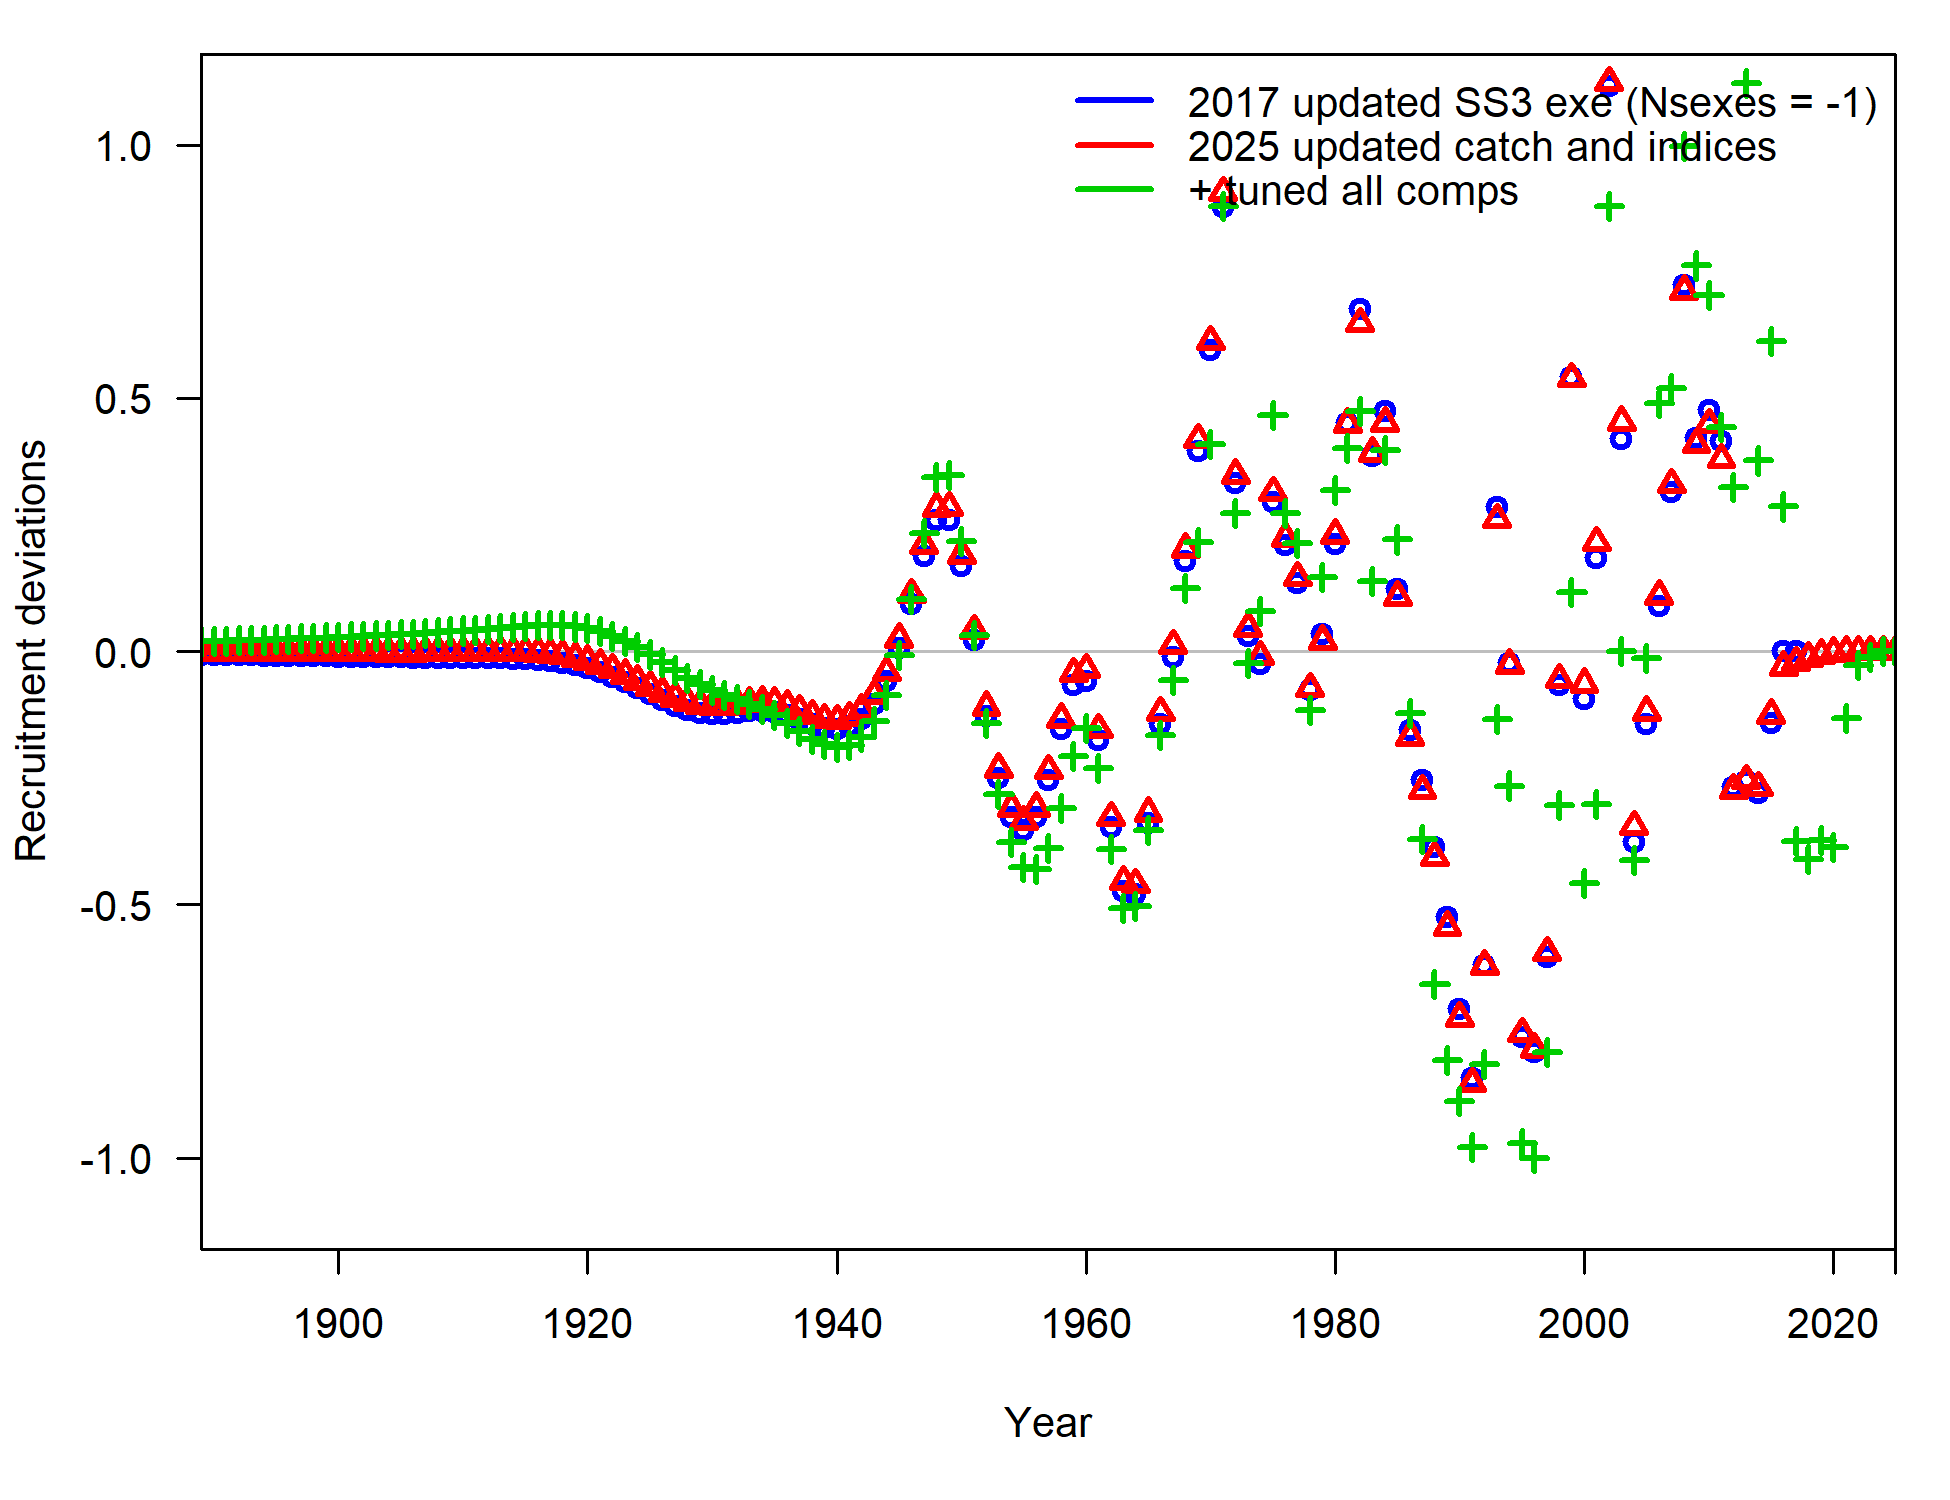
\includegraphics{figures/bridging/14_tunecomps/compare11_recdevs.png}

}

\caption{\label{fig-bridge14-comp11}Recruitment deviation time-series
comparing an updated SS3 executable (blue), updated and extended catch
and indices (red), and all tuned length and age composition data
(green).}

\end{figure}%

\begin{figure}

\centering{

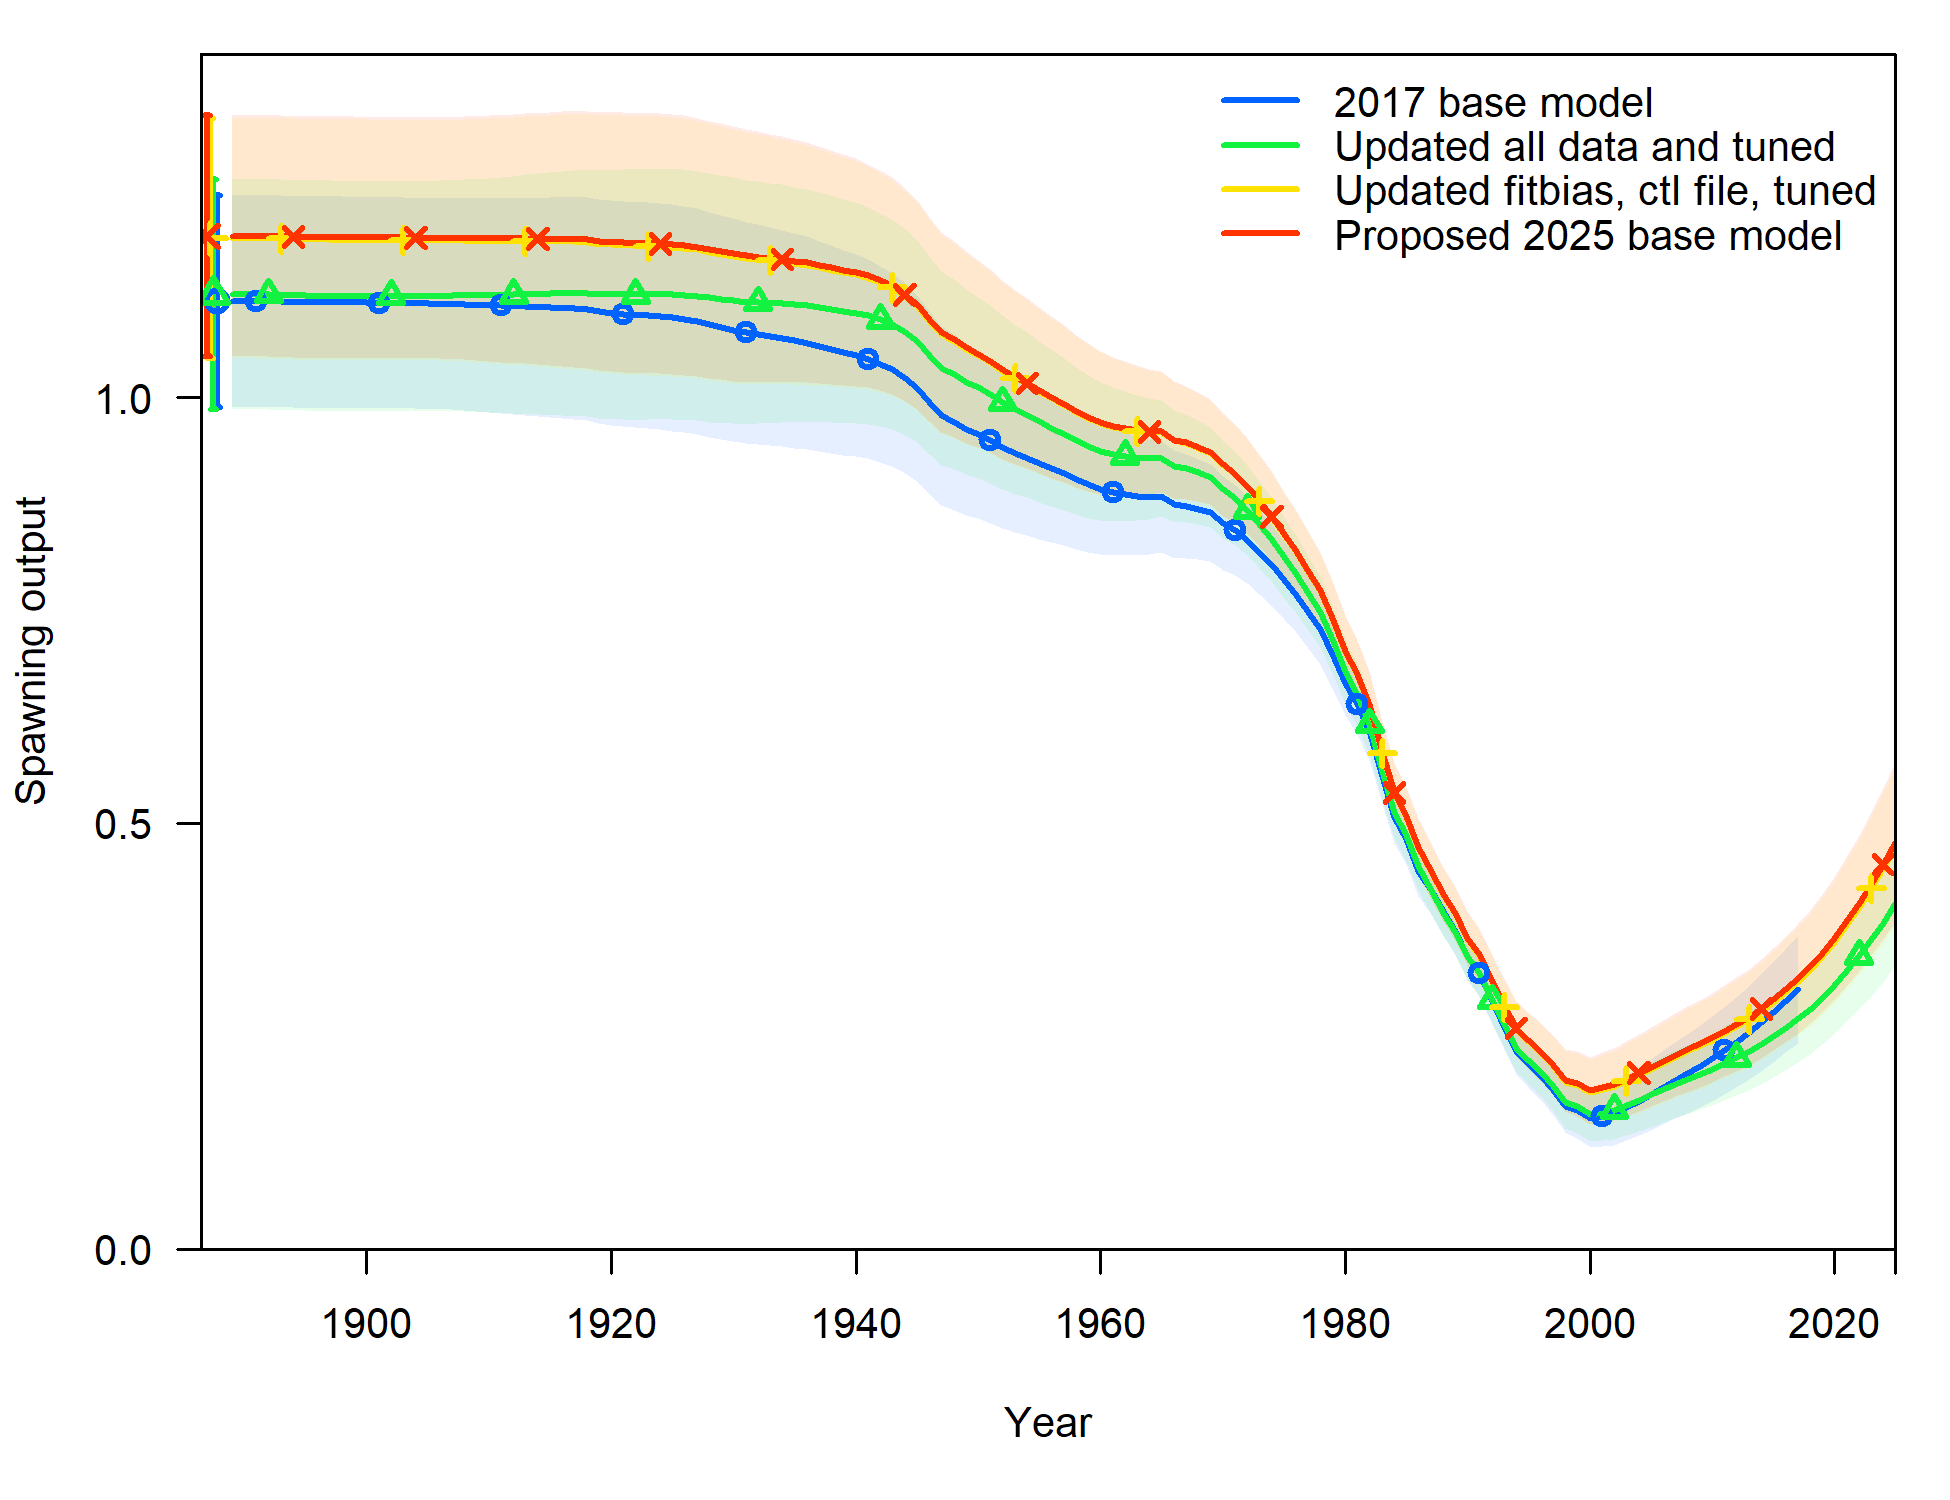
\includegraphics{figures/bridging/23_alldata_tunecomps_fitbias_upctl_tuned_upstart_refine_fore/compare2_spawnbio_uncertainty.png}

}

\caption{\label{fig-bridge23-comp2}Comparison of the spawning output
(millions of eggs) of the 2017 model with an updated SS3 executable
(blue), updated and extended and tuned data (green), the updated SS
input file changes with tuning (yellow), and the proposed 2025 base
model after all final bridging steps (red), all with 95\% confidence
intervals.}

\end{figure}%

\begin{figure}

\centering{

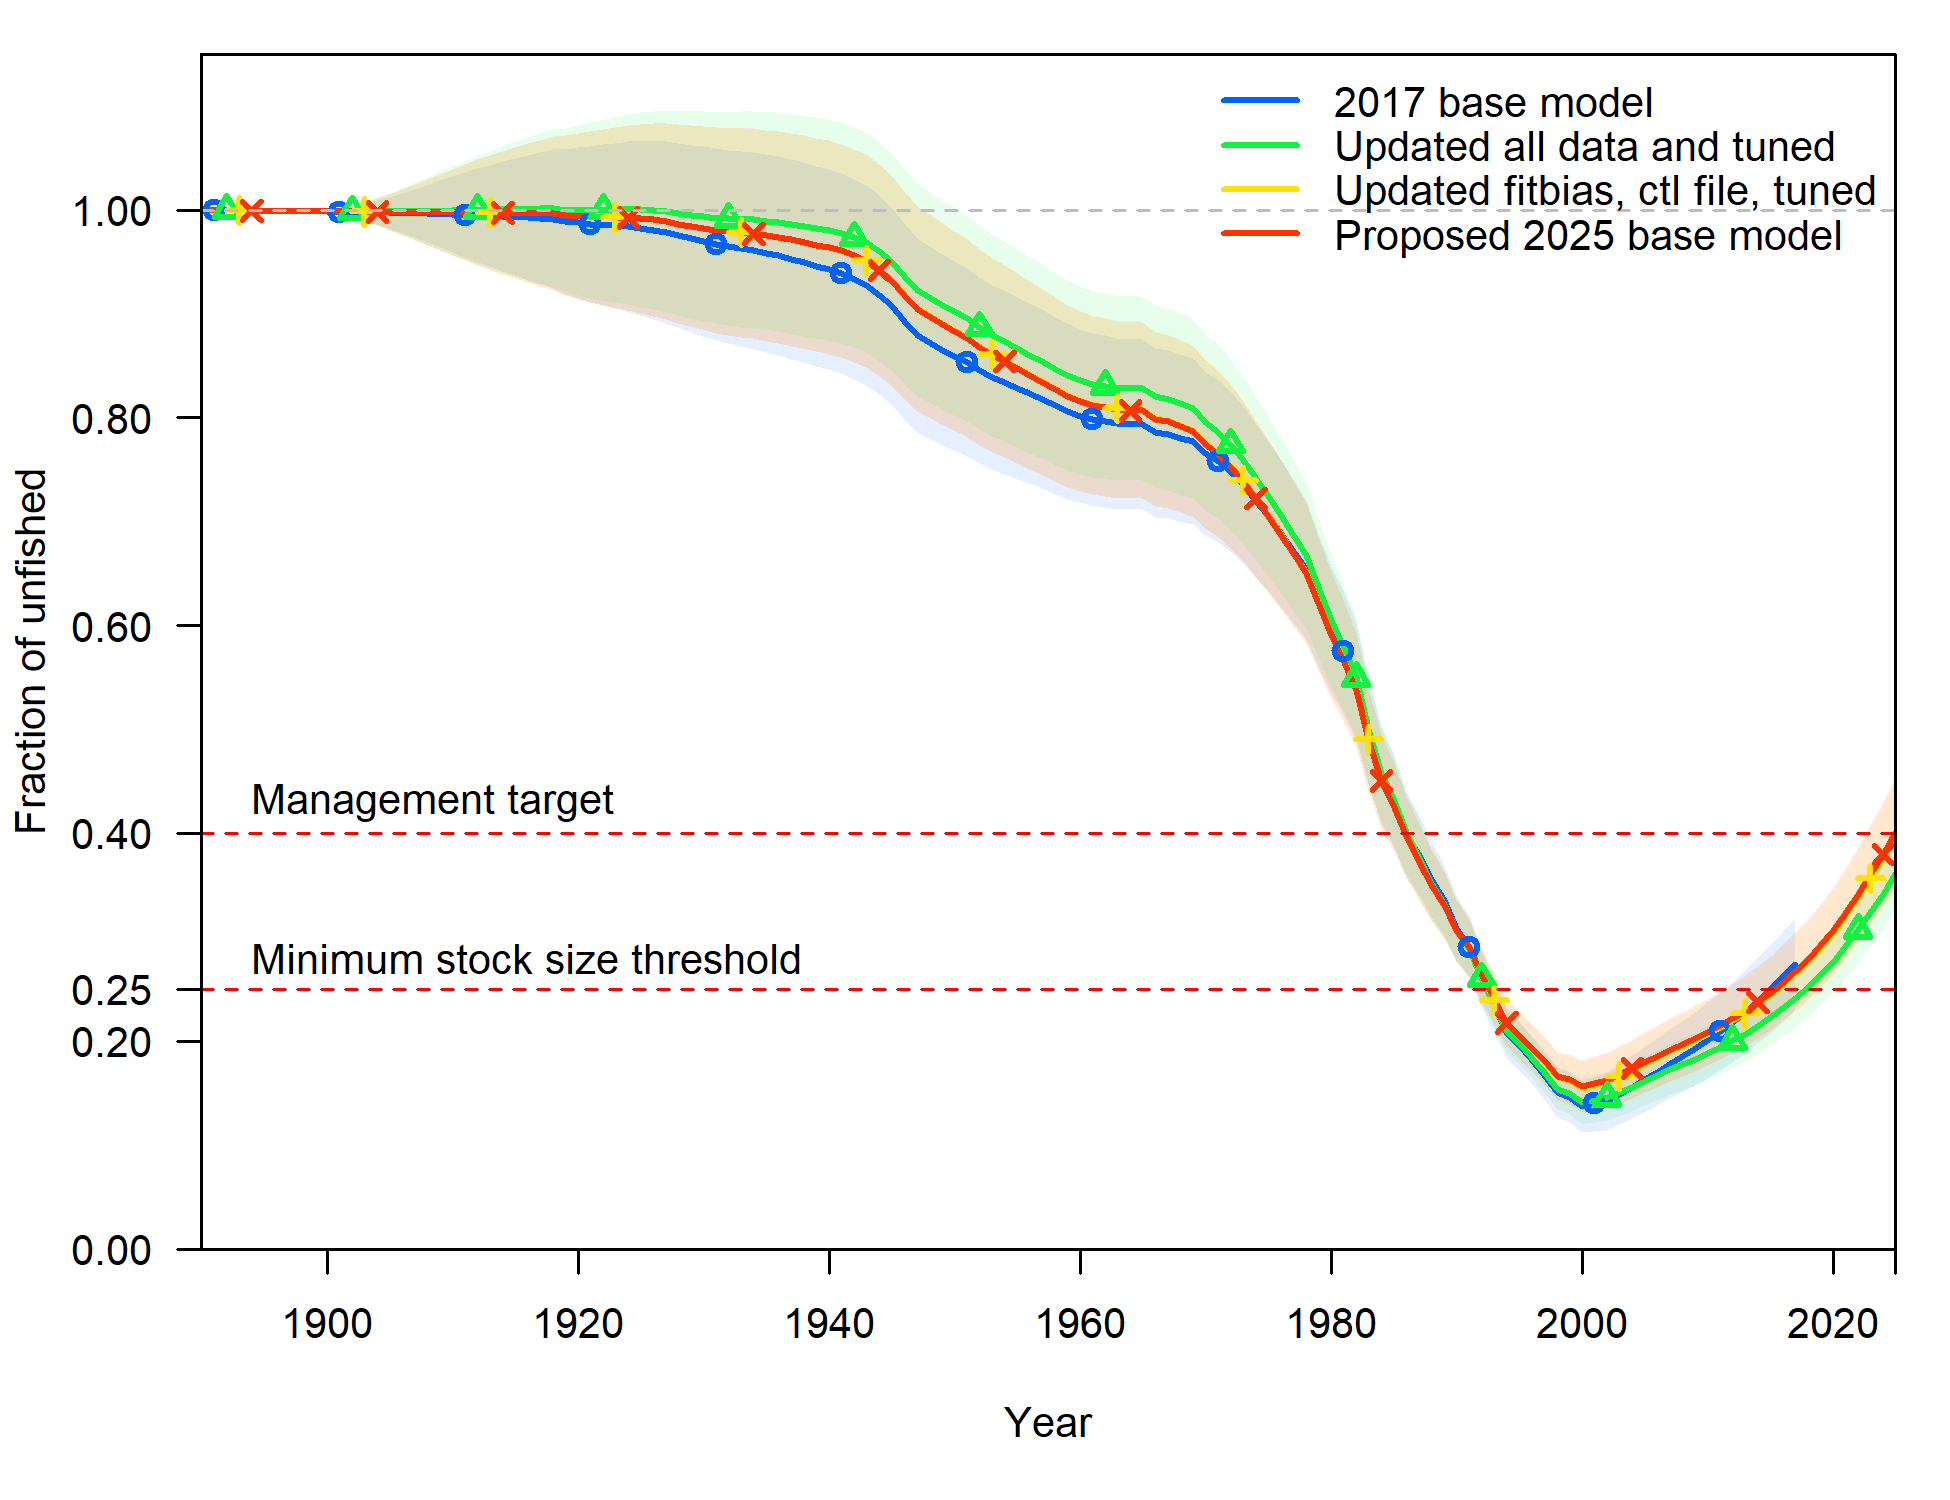
\includegraphics{figures/bridging/23_alldata_tunecomps_fitbias_upctl_tuned_upstart_refine_fore/compare4_Bratio_uncertainty.png}

}

\caption{\label{fig-bridge23-comp4}Comparison of the stock status output
of the 2017 model with an updated SS3 executable (blue), updated and
extended and tuned data (green), the updated SS input file changes with
tuning (yellow), and the proposed 2025 base model after all final
bridging steps (red) relative to the management target and minimum stock
size threshold, including 95\% confidence intervals.}

\end{figure}%

\begin{figure}

\centering{

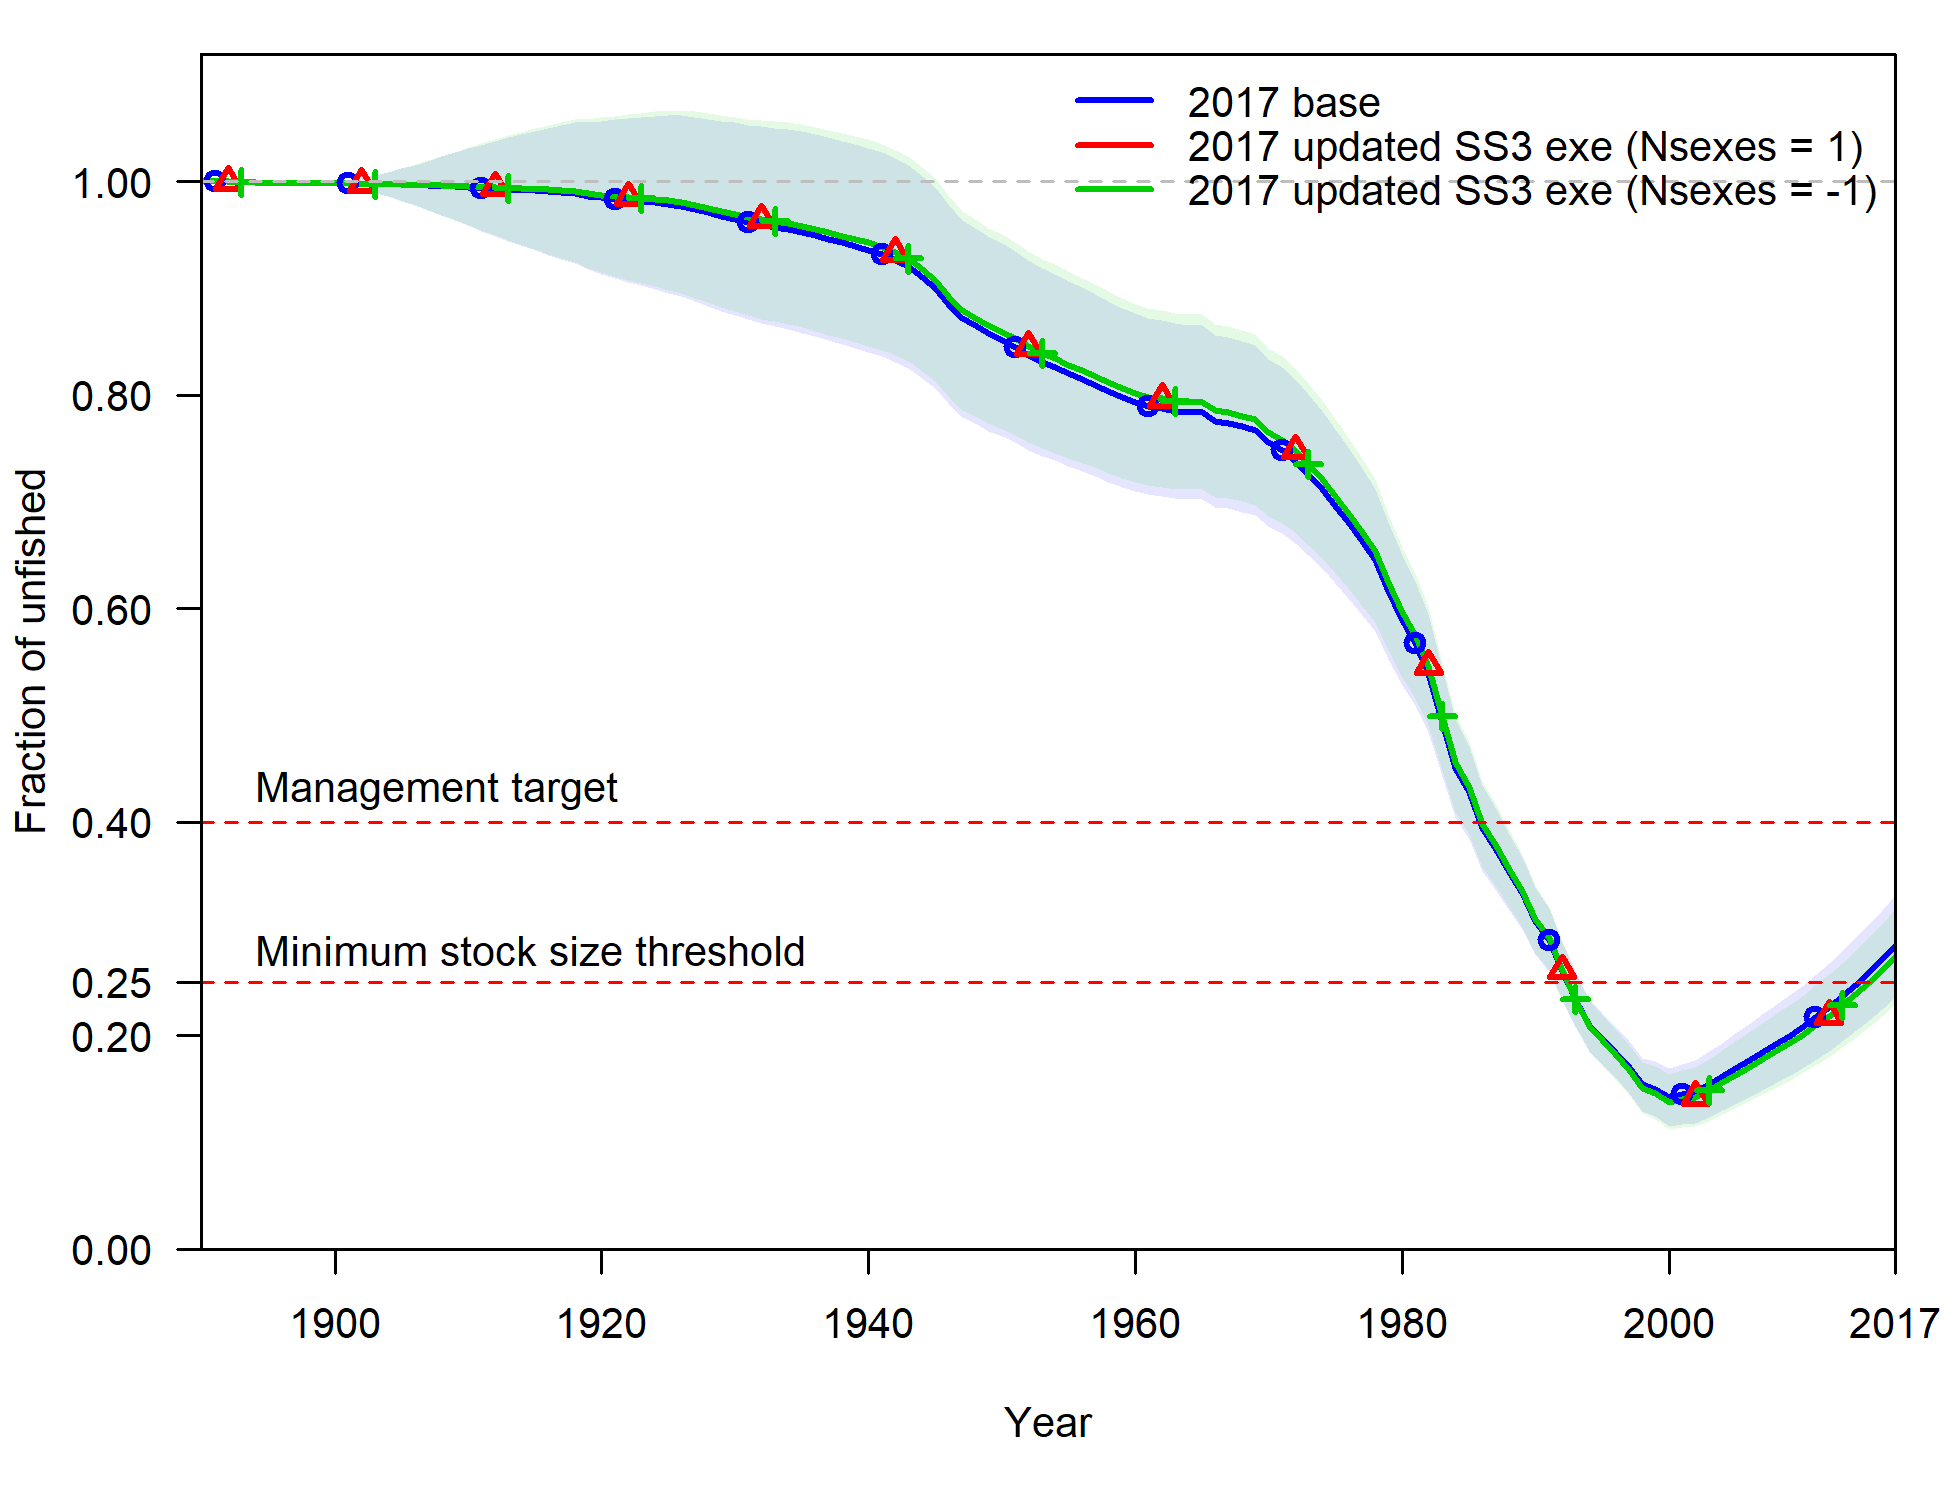
\includegraphics{figures/bridging/1_SS3exe/compare4_Bratio_uncertainty.png}

}

\caption{\label{fig-ss3exe_2}Comparison of the stock status for the 2017
model with the updated SS3 executable and a single-sex model.}

\end{figure}%

\clearpage

\begin{figure}

\centering{

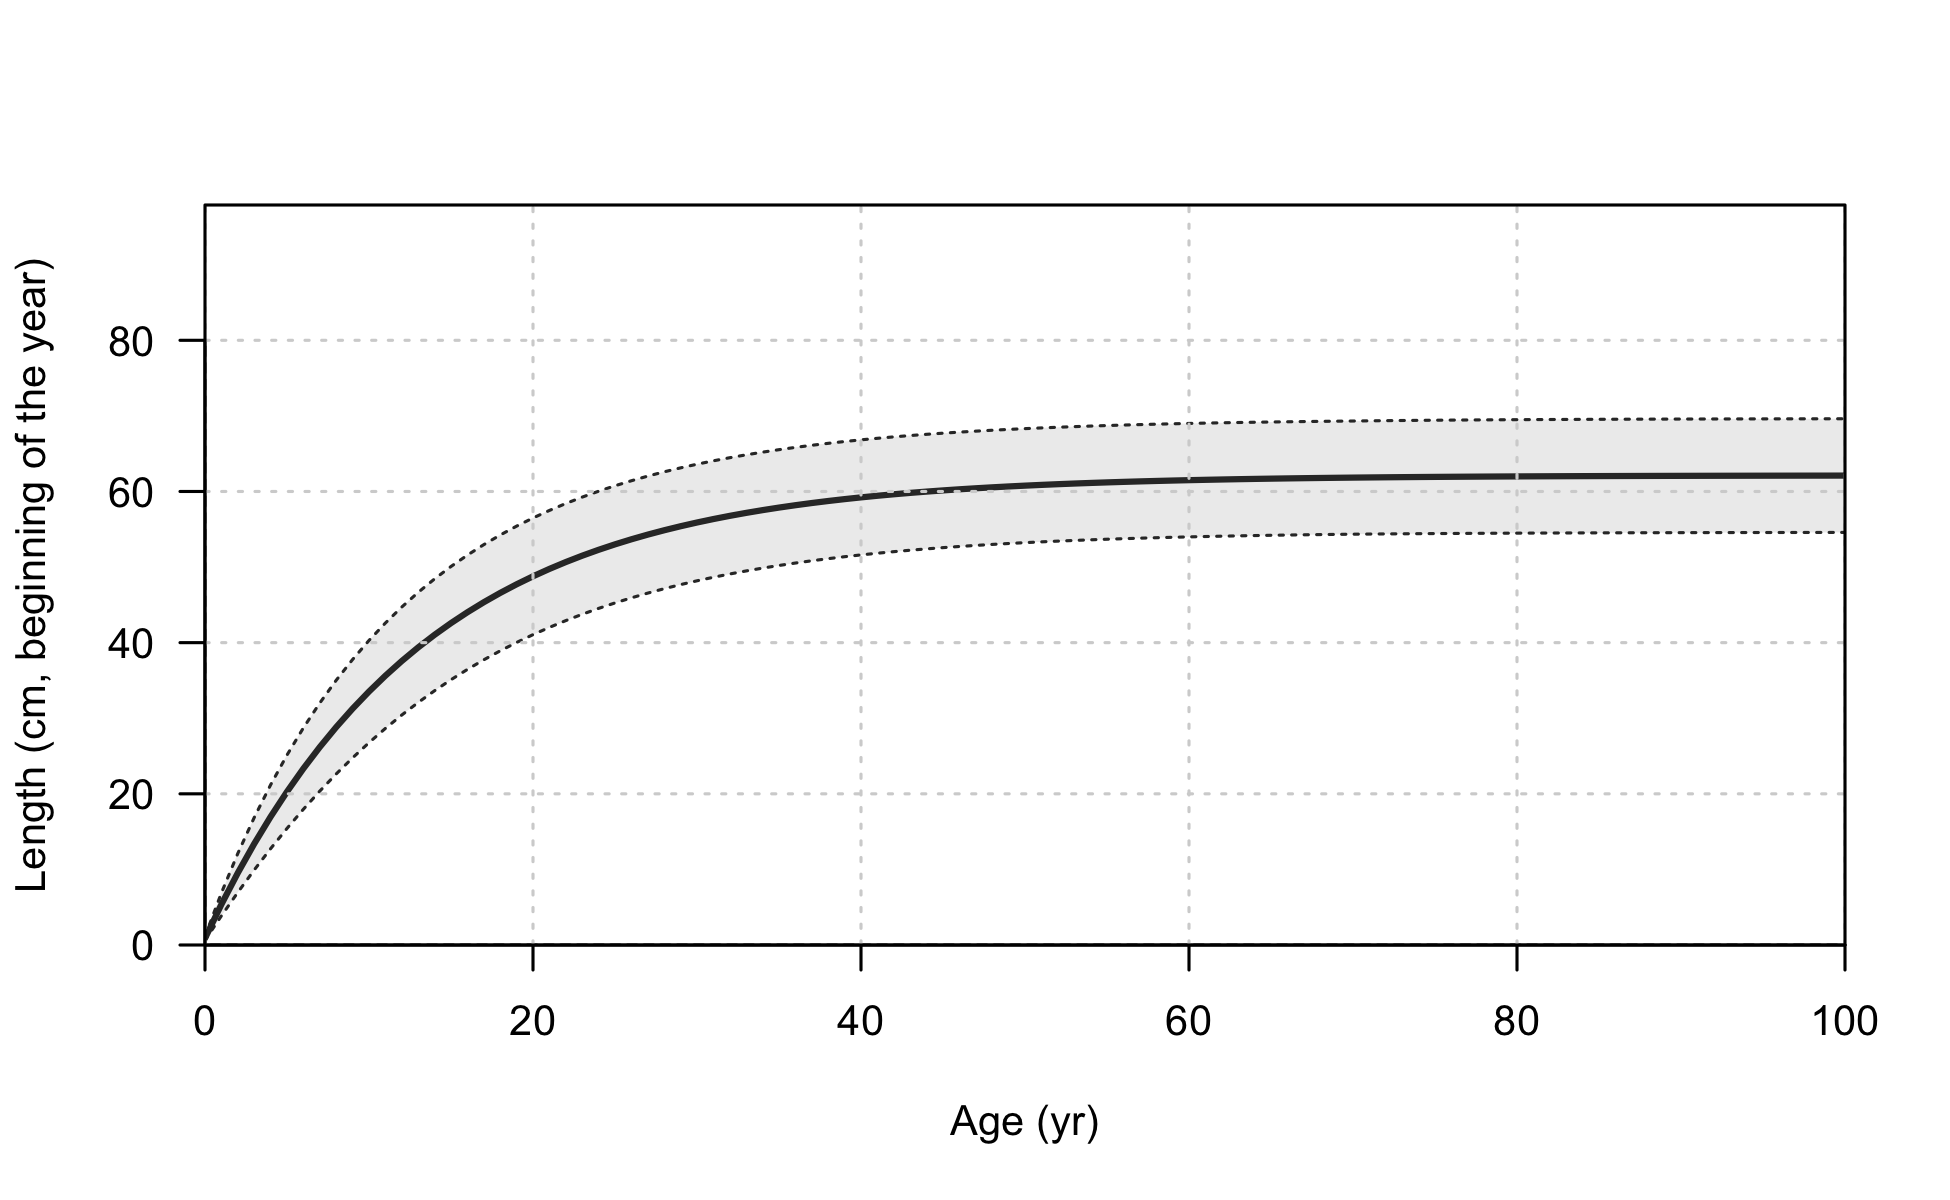
\includegraphics{figures/r4ss_plots/plots/bio1_sizeatage.png}

}

\caption{\label{fig-growth}Length at age in the beginning of the year in
the ending year of the model.}

\end{figure}%

\begin{figure}

\centering{

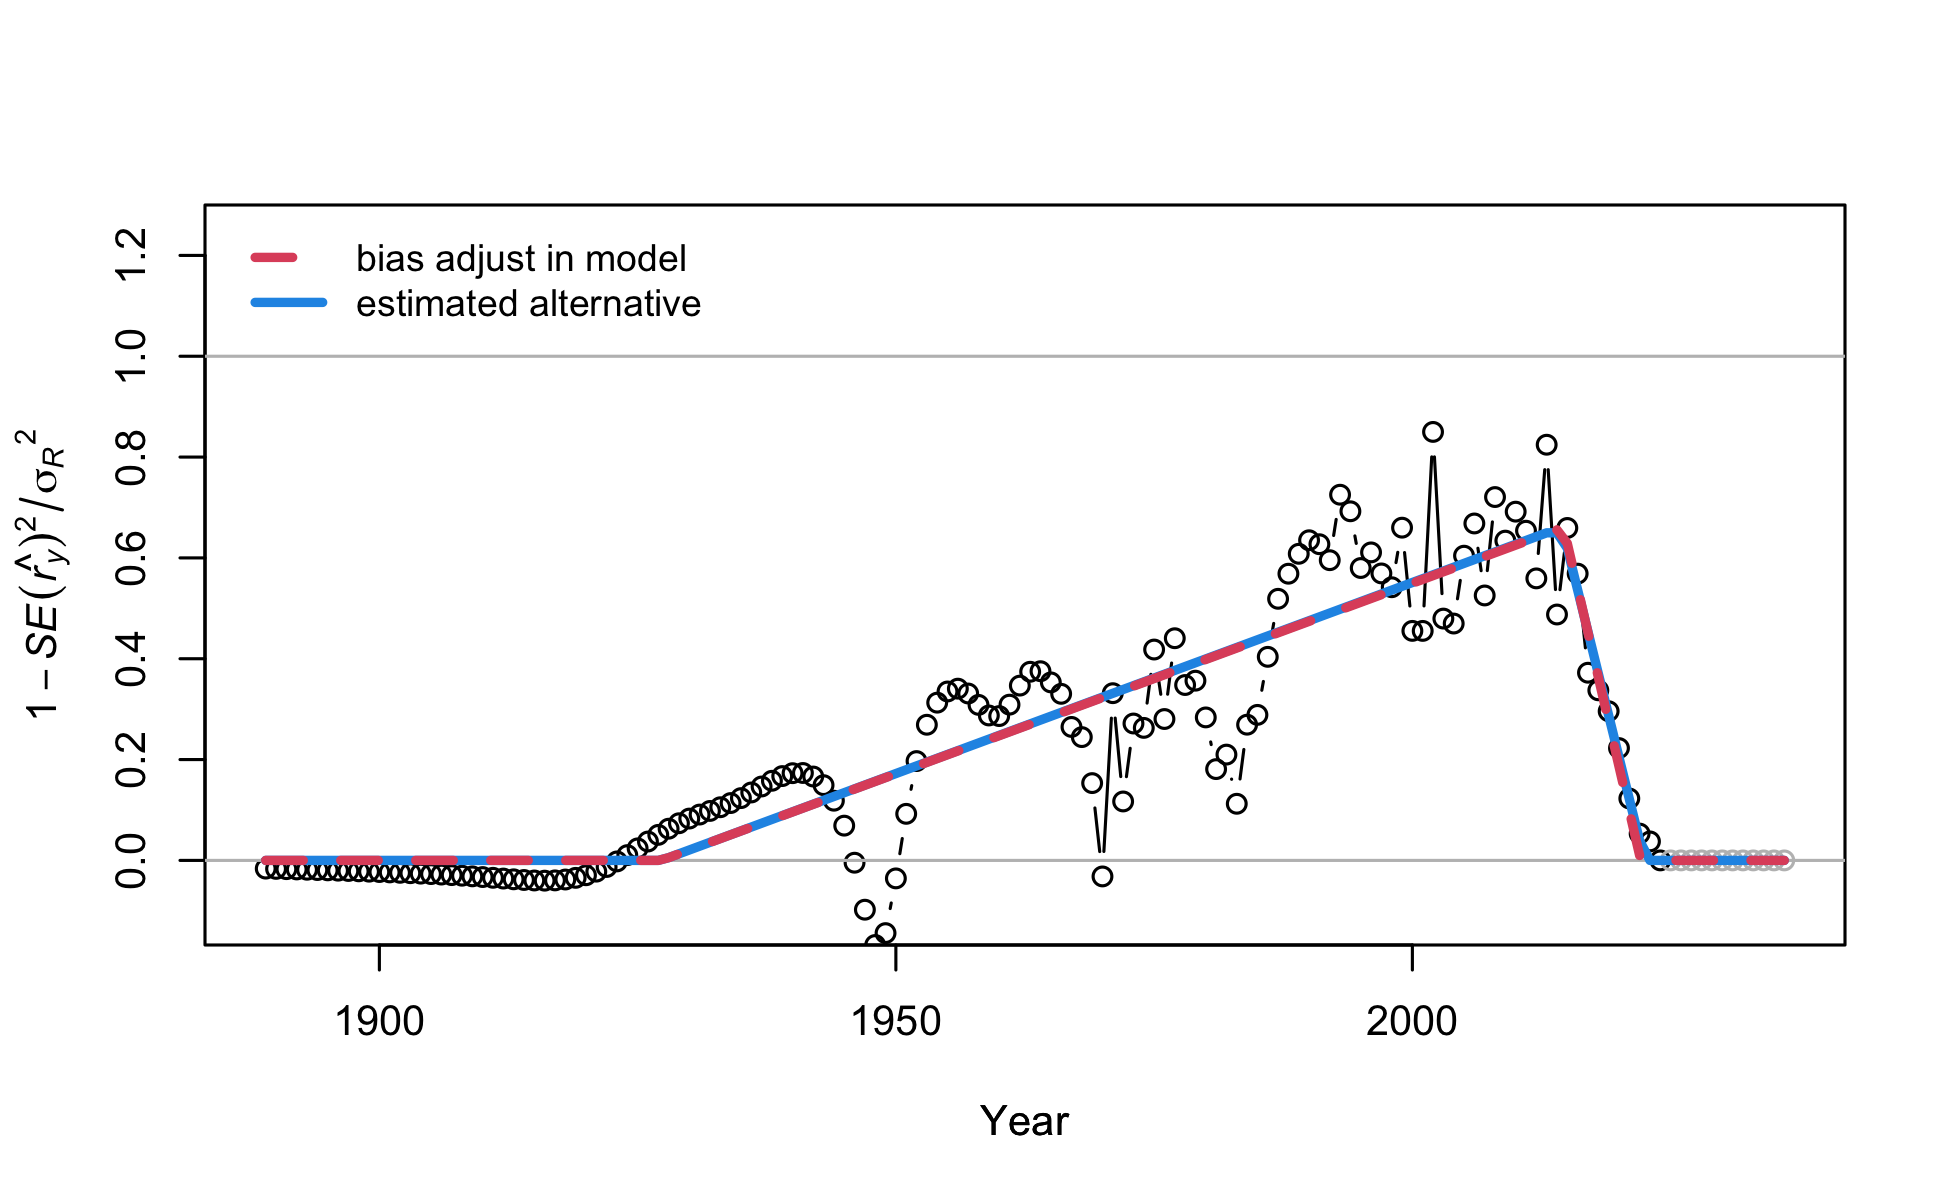
\includegraphics{figures/r4ss_plots/plots/recruit_fit_bias_adjust.png}

}

\caption{\label{fig-biasadj}Points are transformed variances. Red line
shows current settings for bias adjustment specified in the control
file. Blue line shows least squares estimate of alternative bias
adjustment relationship for recruitment deviations.}

\end{figure}%

\clearpage

\begin{figure}

\centering{

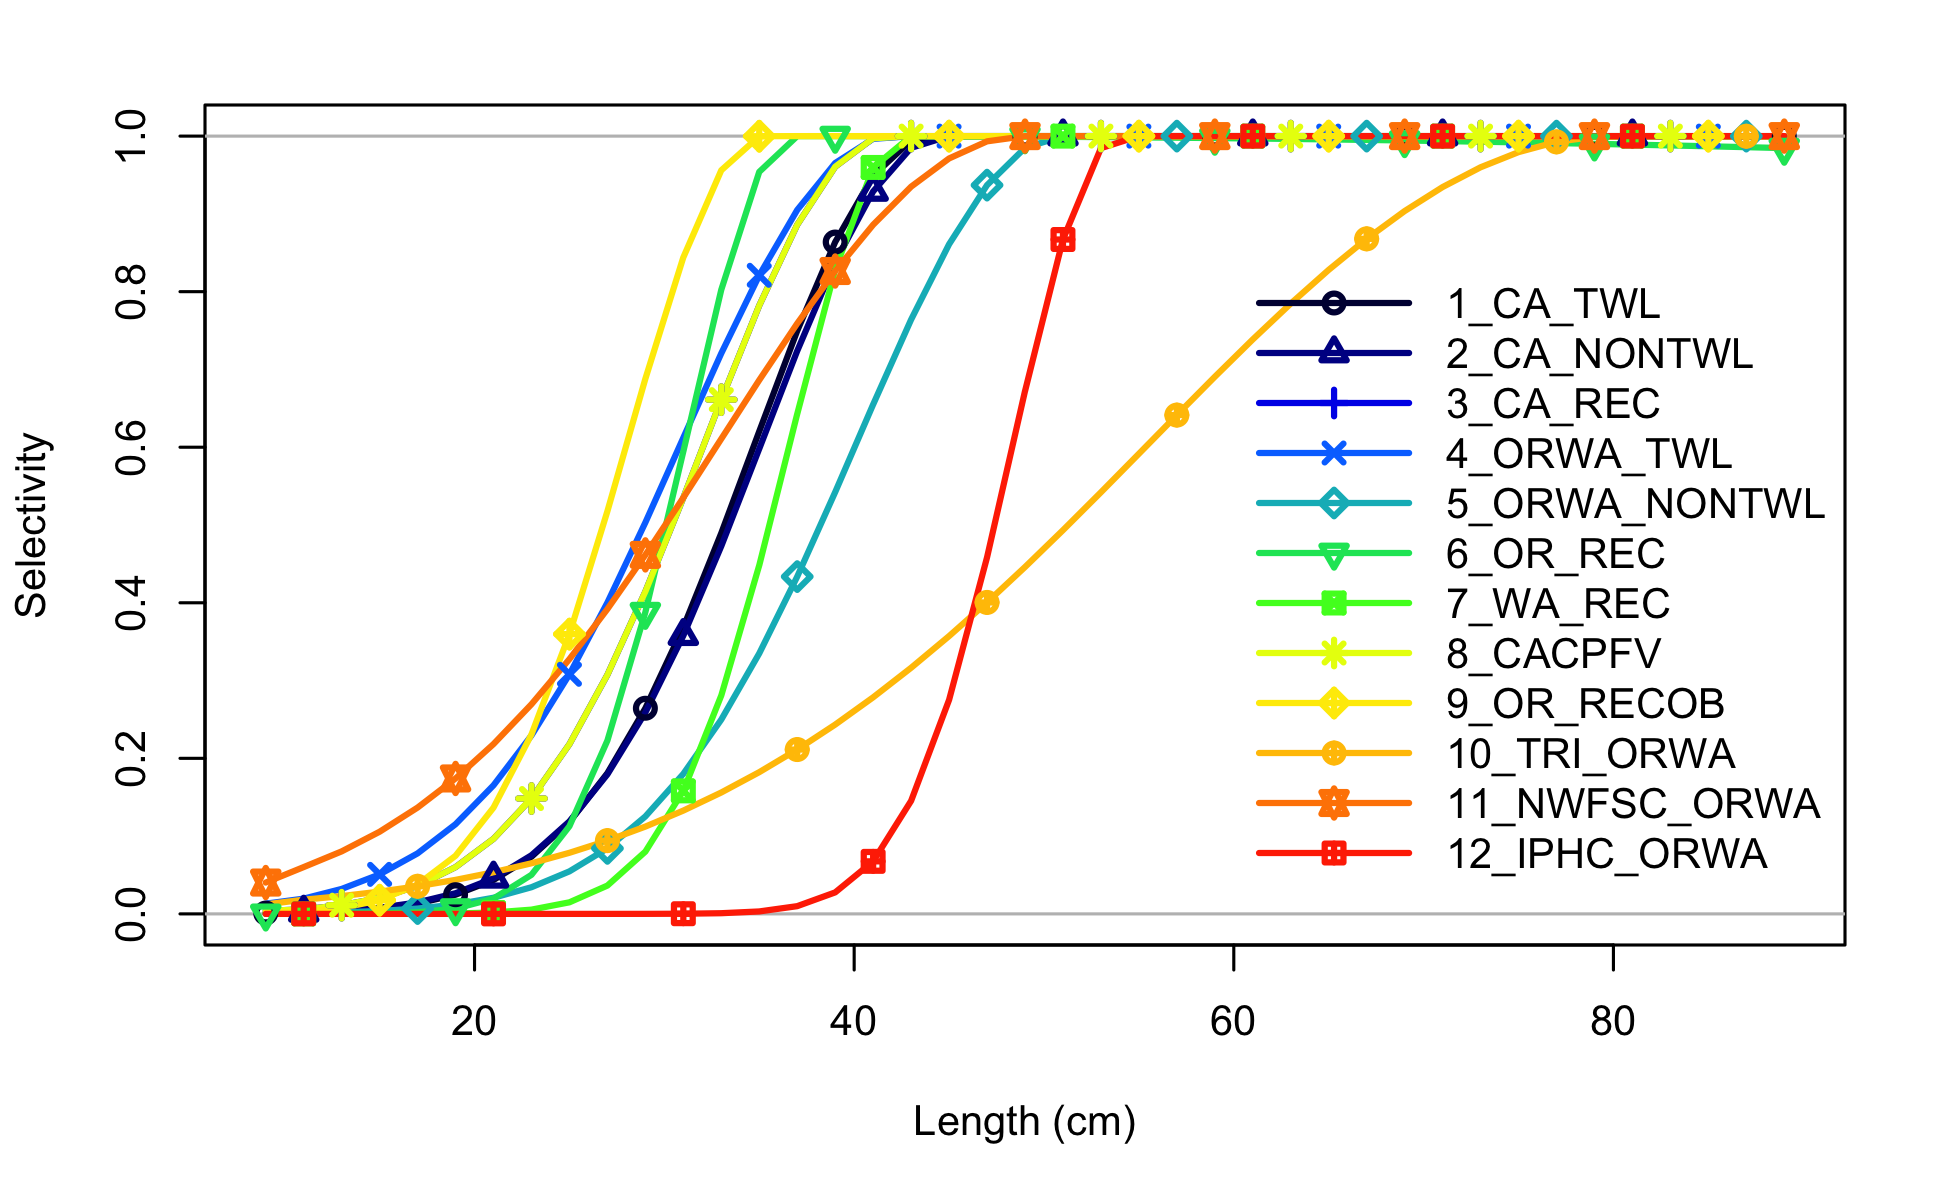
\includegraphics{figures/r4ss_plots/plots/sel01_multiple_fleets_length1.png}

}

\caption{\label{fig-selex_allfleets}Estimated selectivity at length for
all fleets.}

\end{figure}%

\begin{figure}

\centering{

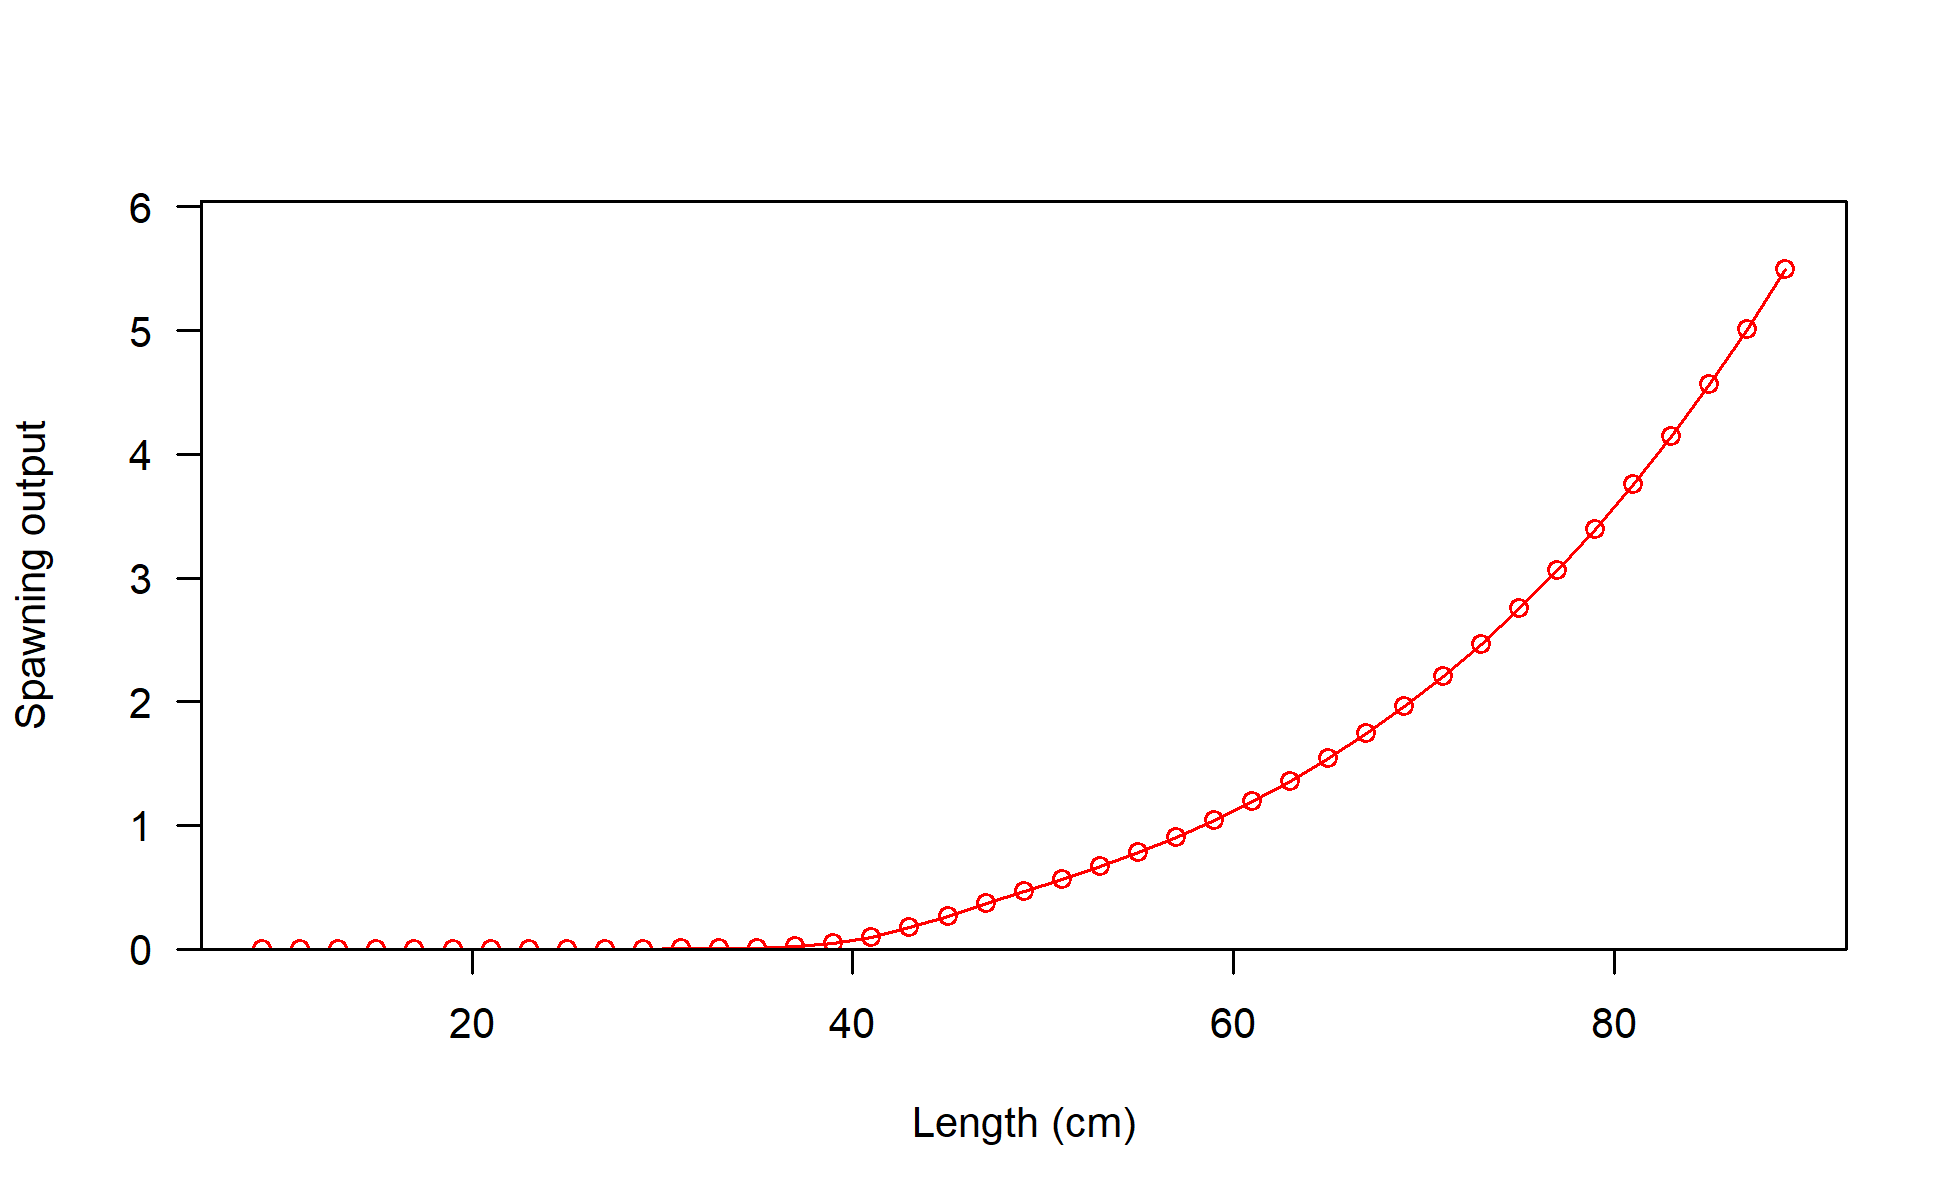
\includegraphics{figures/r4ss_plots/plots/bio10_spawningoutput_len.png}

}

\caption{\label{fig-spoutlen}Spawning output (millions of eggs) at
length. Yelloweye length-at-age 70 (the second reference age) equals
61.4 and an L-infinity of 61.7.}

\end{figure}%

\begin{figure}

\centering{

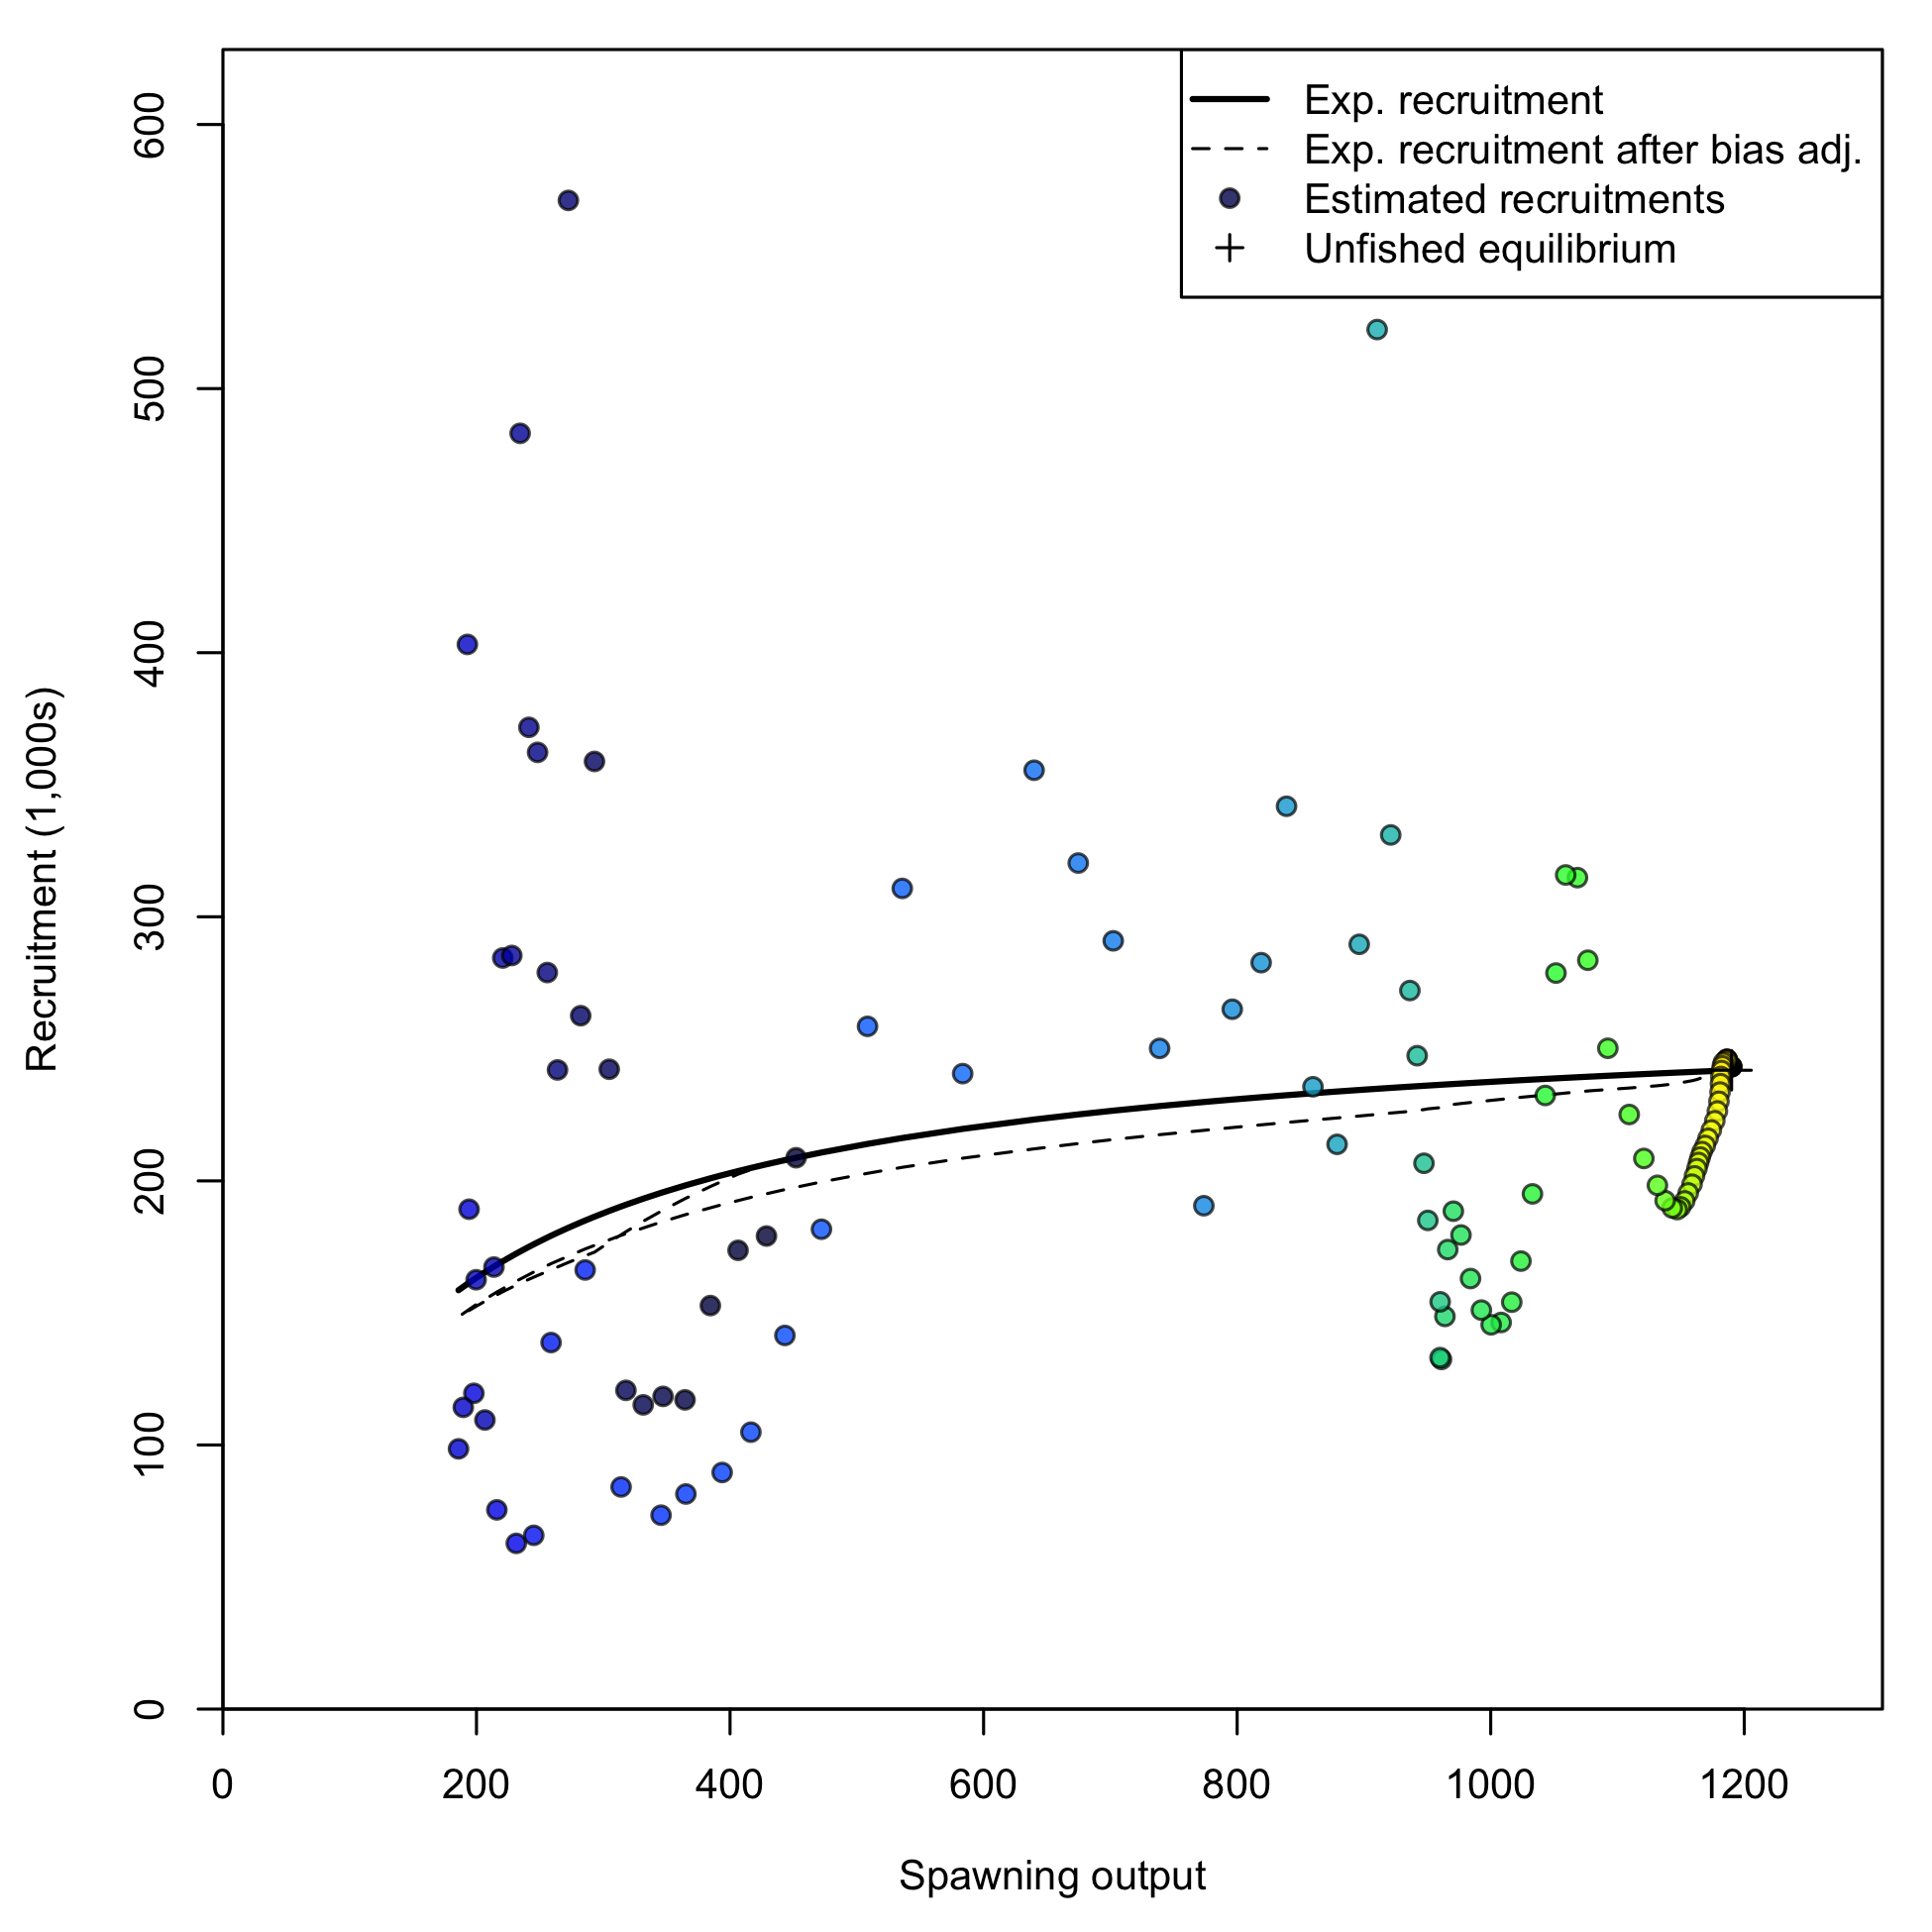
\includegraphics{figures/r4ss_plots/plots/SR_curve.png}

}

\caption{\label{fig-SRcurve}Stock-recruit curve. Point colors indicate
year, with warmer colors indicating earlier years and cooler colors in
showing later years.}

\end{figure}%

\begin{figure}

\centering{

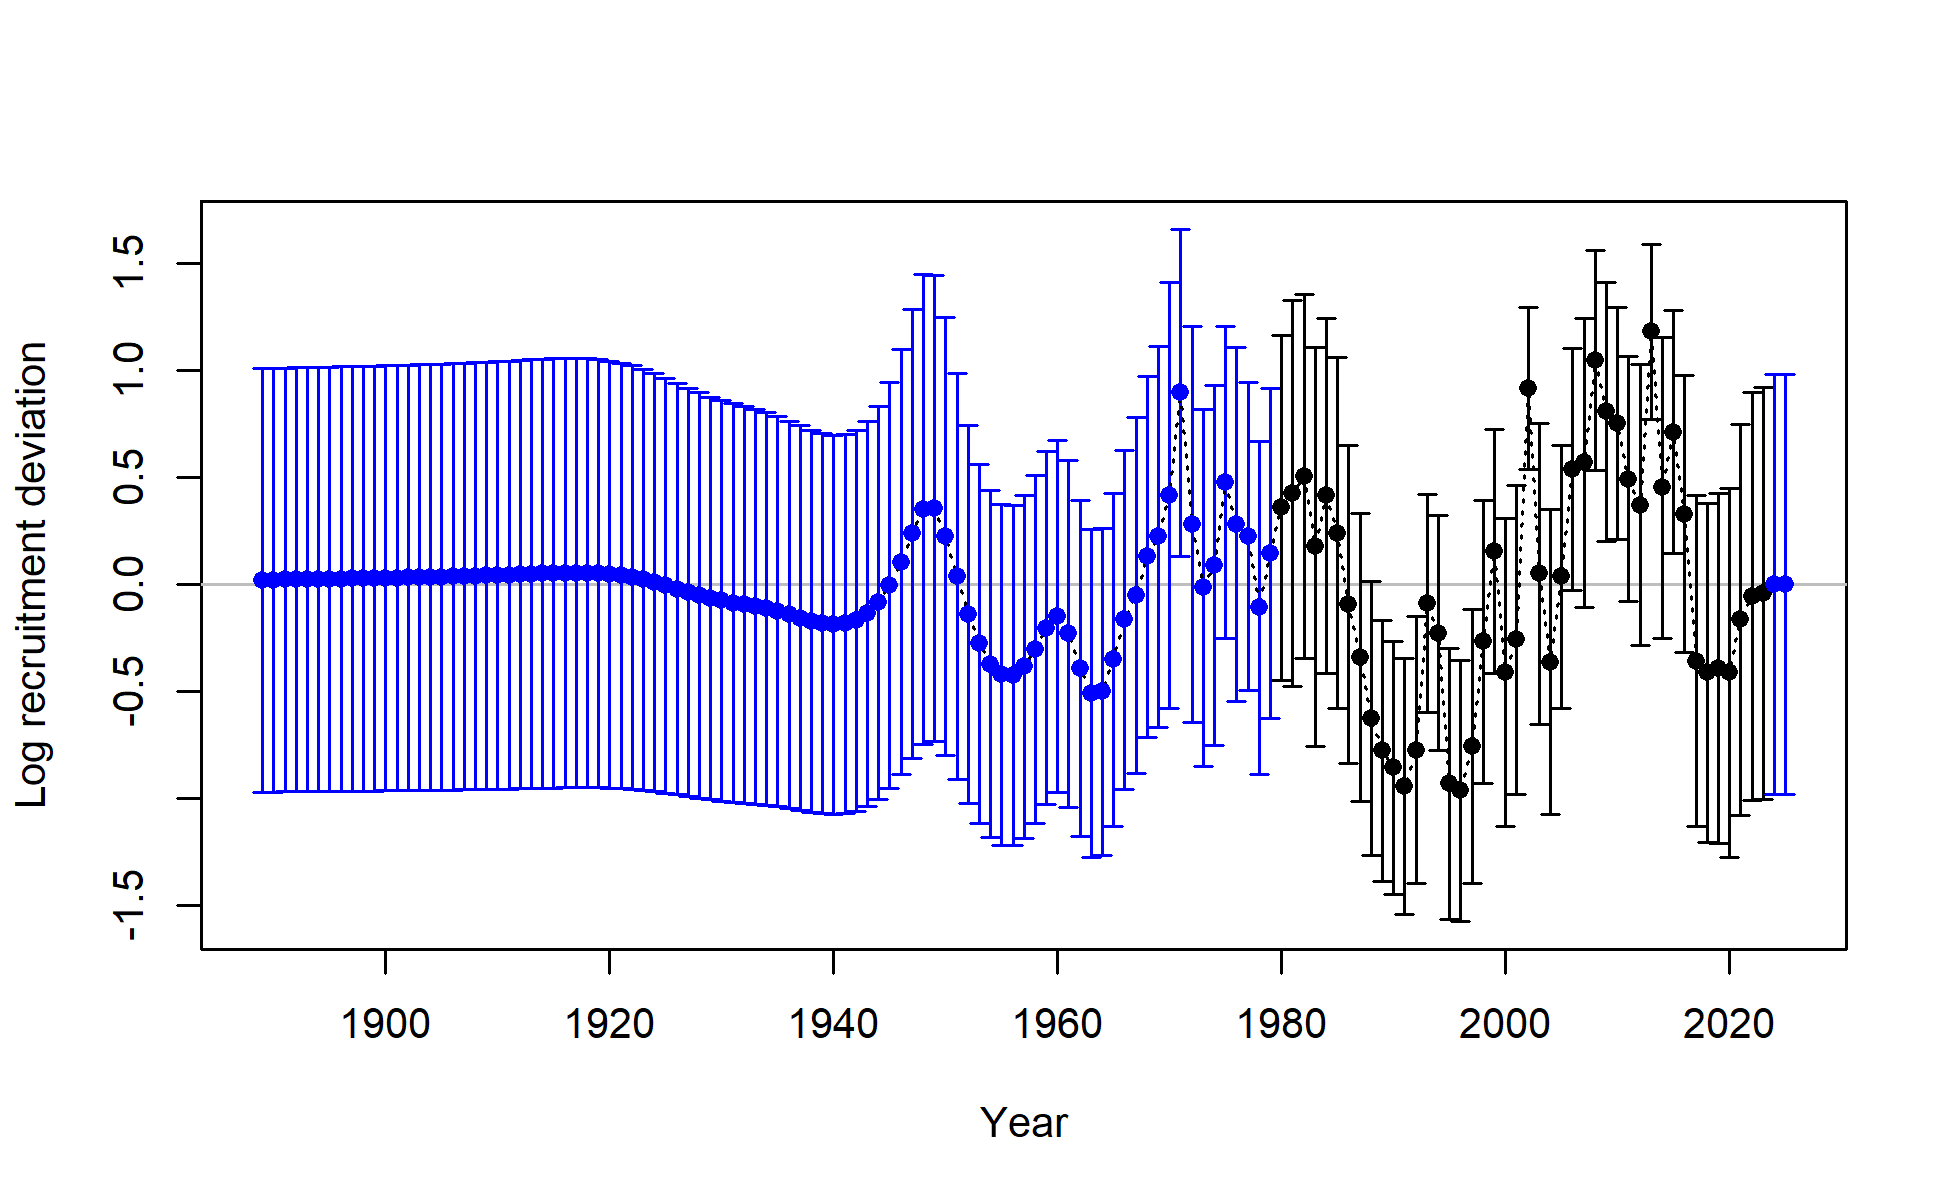
\includegraphics{figures/r4ss_plots/plots/recdevs2_withbars.png}

}

\caption{\label{fig-recdevs_err}Estimated recruitment deviations with
95\% intervals.}

\end{figure}%

\clearpage

\begin{figure}

\centering{

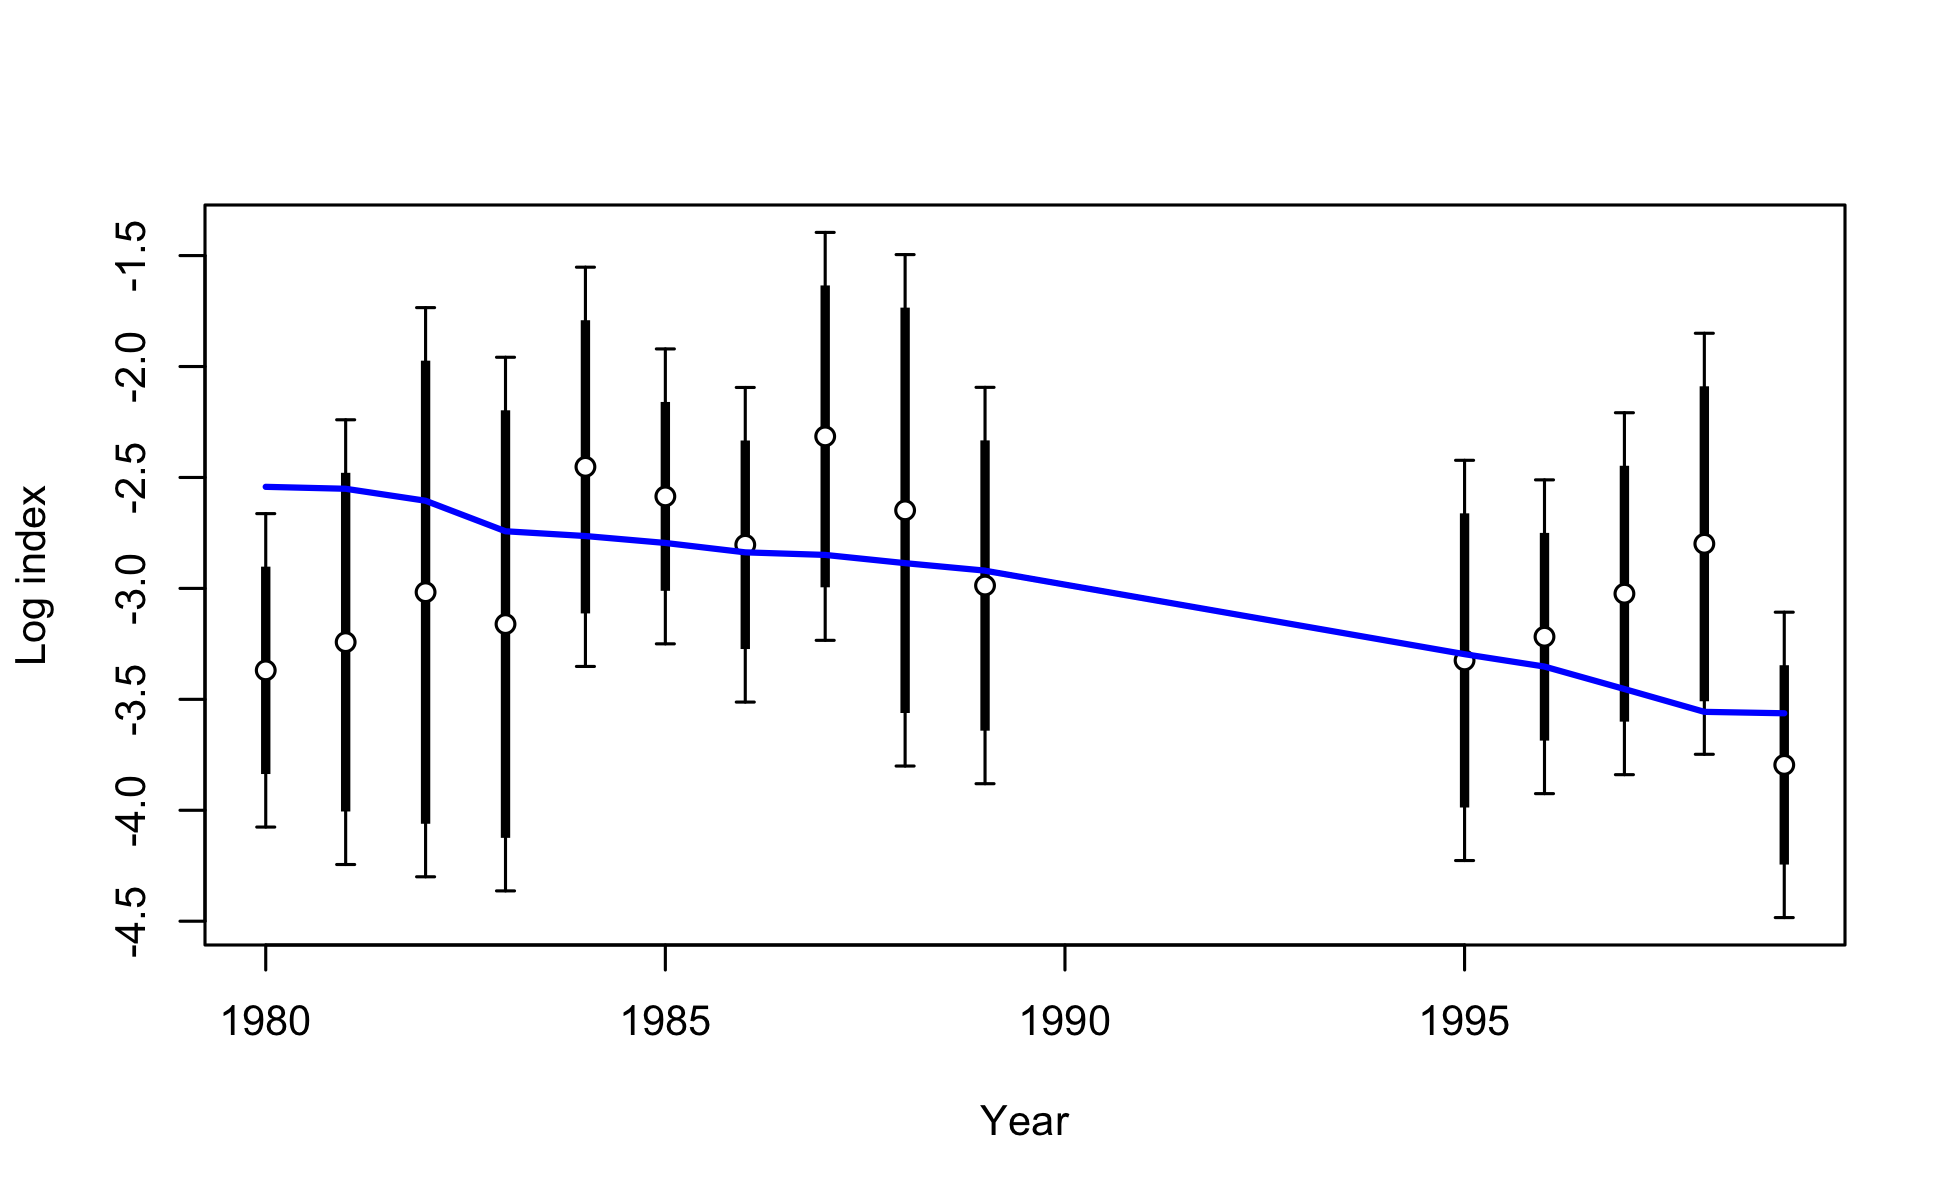
\includegraphics{figures/r4ss_plots/plots/index5_logcpuefit_3_CA_REC.png}

}

\caption{\label{fig-indexfit3}Fit to the California MRFSS recreational
index.}

\end{figure}%

\begin{figure}

\centering{

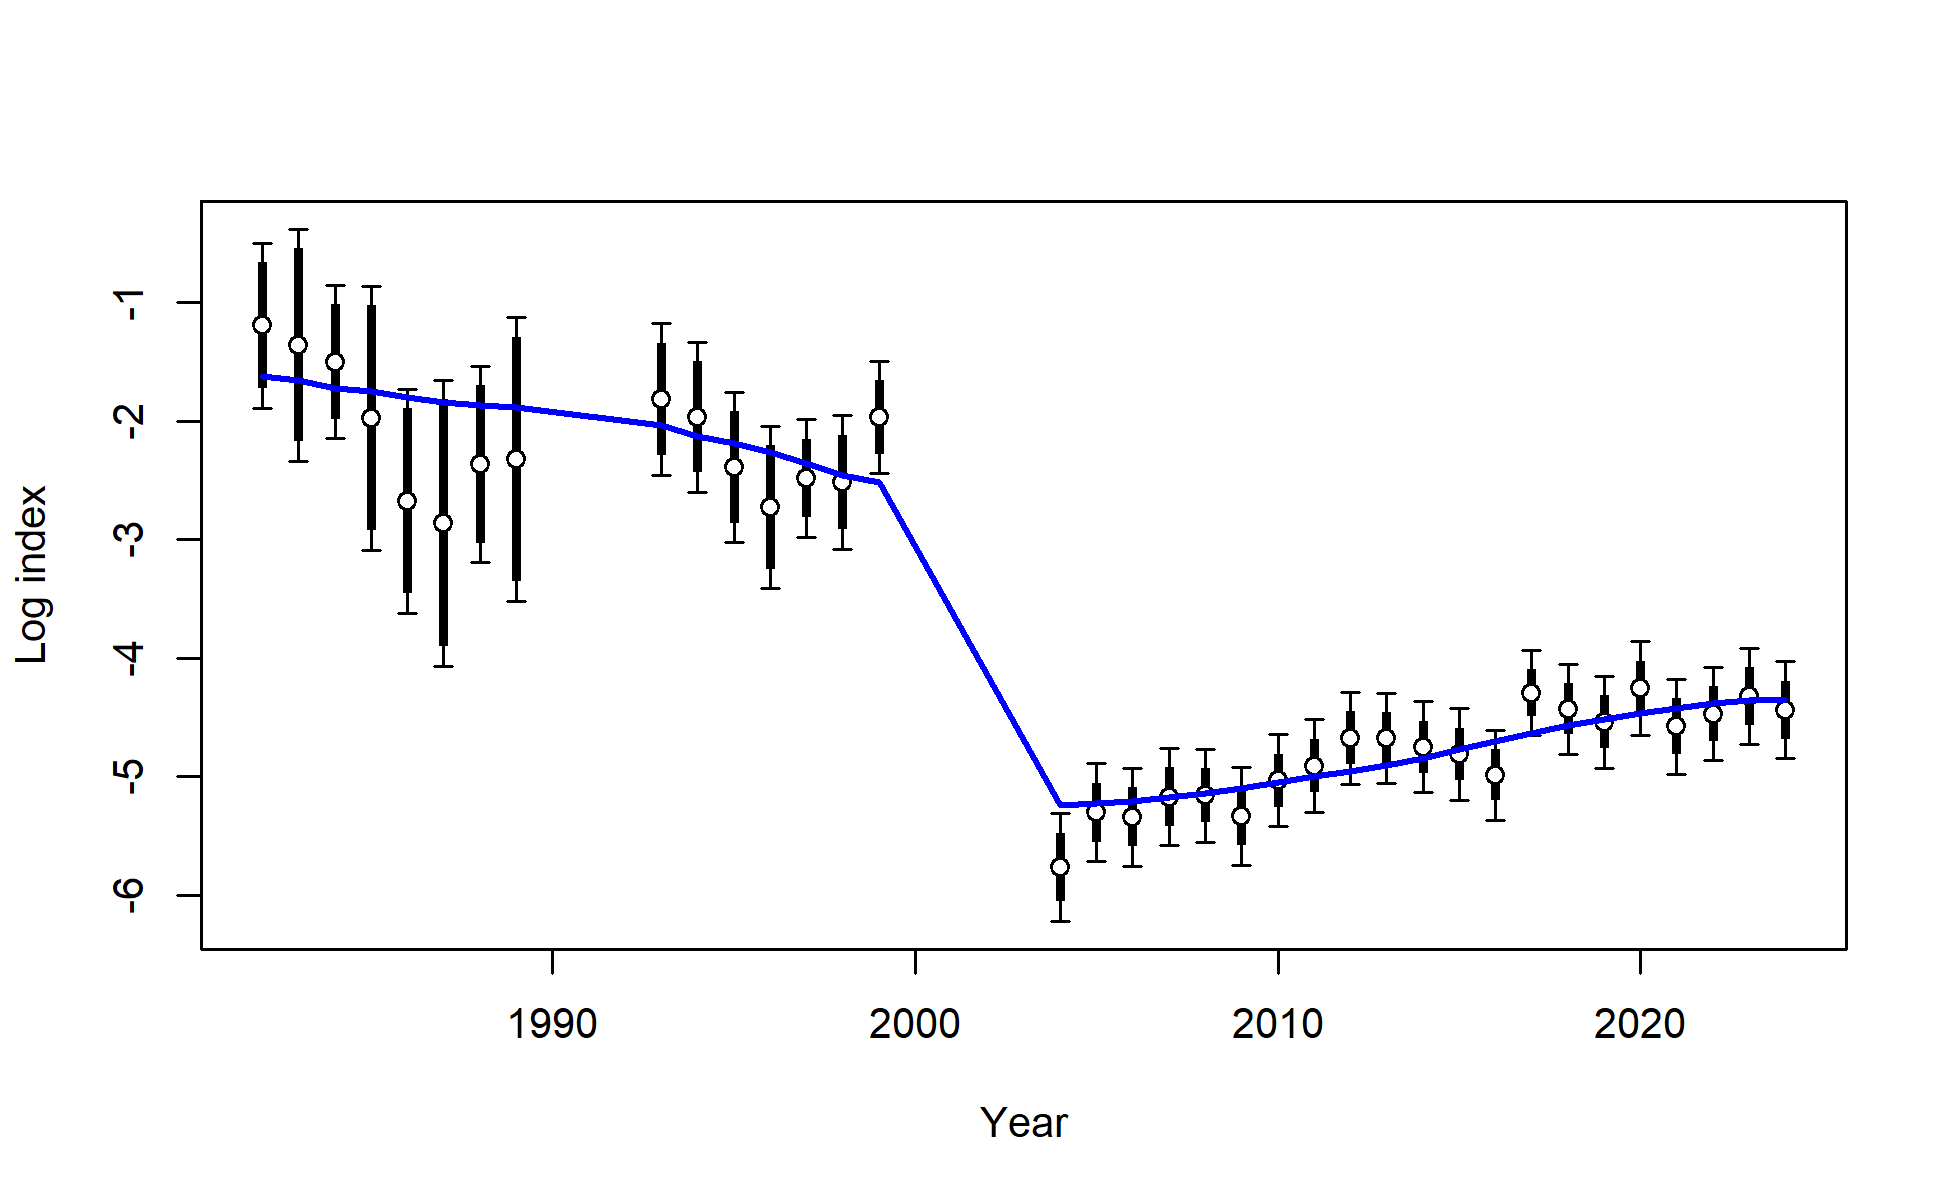
\includegraphics{figures/r4ss_plots/plots/index5_logcpuefit_6_OR_REC.png}

}

\caption{\label{fig-indexfit6}Fit to the Oregon recreational index.}

\end{figure}%

\begin{figure}

\centering{

\includegraphics{figures/r4ss_plots/plots/index5_logcpuefit_7_WA_REC.png}

}

\caption{\label{fig-indexfit7}Fit to the Washington recreational index.}

\end{figure}%

\begin{figure}

\centering{

\includegraphics{figures/r4ss_plots/plots/index5_logcpuefit_8_CACPFV.png}

}

\caption{\label{fig-indexfit8}Fit to the California CPFV observer
index.}

\end{figure}%

\begin{figure}

\centering{

\includegraphics{figures/r4ss_plots/plots/index5_logcpuefit_9_OR_RECOB.png}

}

\caption{\label{fig-indexfit9}Fit to the Oregon onboard observer (ORFS)
index.}

\end{figure}%

\begin{figure}

\centering{

\includegraphics{figures/r4ss_plots/plots/index5_logcpuefit_10_TRI_ORWA.png}

}

\caption{\label{fig-indexfit10}Fit to the Triennial survey index.}

\end{figure}%

\begin{figure}

\centering{

\includegraphics{figures/r4ss_plots/plots/index5_logcpuefit_11_NWFSC_ORWA.png}

}

\caption{\label{fig-indexfit11}Fit to the WCBTS index.}

\end{figure}%

\begin{figure}

\centering{

\includegraphics{figures/r4ss_plots/plots/index5_logcpuefit_12_IPHC_ORWA.png}

}

\caption{\label{fig-indexfit12}Fit to the IPHC survey index.}

\end{figure}%

\clearpage

\begin{figure}

\centering{

\includegraphics{figures/r4ss_plots/plots/comp_lenfit__aggregated_across_time.png}

}

\caption{\label{fig-agglencomps}Fit to length composition data,
aggregated across time by fleet.}

\end{figure}%

\begin{figure}

\centering{

\includegraphics{figures/r4ss_plots/plots/comp_lenfit__page1_multi-fleet_comparison.png}

}

\caption{\label{fig-pearsonlenfit1}Pearson residuals, comparing across
fleets, for length composition data (1 of 2). Closed bubbles are
positive residuals (observed \textgreater{} expected) and open bubbles
are negative residuals (observed \textless{} expected).}

\end{figure}%

\begin{figure}

\centering{

\includegraphics{figures/r4ss_plots/plots/comp_lenfit__page2_multi-fleet_comparison.png}

}

\caption{\label{fig-pearsonlenfit2}Pearson residuals, comparing across
fleets, for length composition data (2 of 2). Closed bubbles are
positive residuals (observed \textgreater{} expected) and open bubbles
are negative residuals (observed \textless{} expected).}

\end{figure}%

\begin{figure}

\centering{

\includegraphics{figures/r4ss_plots/plots/comp_condAALfit_data_weighting_TA1-8_condAge2_CA_NONTWL.png}

}

\caption{\label{fig-mean-age-2}Mean age from conditional data
(aggregated across length bins) for the CA NONTWL fleet with 95\%
confidence intervals based on input sample sizes. The blue line is the
model expectation.}

\end{figure}%

\begin{figure}

\centering{

\includegraphics{figures/r4ss_plots/plots/comp_condAALfit_data_weighting_TA1-8_condAge3_CA_REC.png}

}

\caption{\label{fig-mean-age-3}Mean age from conditional data
(aggregated across length bins) for the CA REC fleet with 95\%
confidence intervals based on input sample sizes. The blue line is the
model expectation.}

\end{figure}%

\begin{figure}

\centering{

\includegraphics{figures/r4ss_plots/plots/comp_condAALfit_data_weighting_TA1-8_condAge4_ORWA_TWL.png}

}

\caption{\label{fig-mean-age-4}Mean age from conditional data
(aggregated across length bins) for the ORWA TWL fleet with 95\%
confidence intervals based on input sample sizes. The blue line is the
model expectation.}

\end{figure}%

\begin{figure}

\centering{

\includegraphics{figures/r4ss_plots/plots/comp_condAALfit_data_weighting_TA1-8_condAge5_ORWA_NONTWL.png}

}

\caption{\label{fig-mean-age-5}Mean age from conditional data
(aggregated across length bins) for the ORWA NONTWL fleet with 95\%
confidence intervals based on input sample sizes. The blue line is the
model expectation.}

\end{figure}%

\begin{figure}

\centering{

\includegraphics{figures/r4ss_plots/plots/comp_condAALfit_data_weighting_TA1-8_condAge6_OR_REC.png}

}

\caption{\label{fig-mean-age-6}Mean age from conditional data
(aggregated across length bins) for the ORWA REC fleet with 95\%
confidence intervals based on input sample sizes. The blue line is the
model expectation.}

\end{figure}%

\begin{figure}

\centering{

\includegraphics{figures/r4ss_plots/plots/comp_condAALfit_data_weighting_TA1-8_condAge7_WA_REC.png}

}

\caption{\label{fig-mean-age-7}Mean age from conditional data
(aggregated across length bins) for the WA REC fleet with 95\%
confidence intervals based on input sample sizes. The blue line is the
model expectation.}

\end{figure}%

\begin{figure}

\centering{

\includegraphics{figures/r4ss_plots/plots/comp_condAALfit_data_weighting_TA1-8_condAge11_NWFSC_ORWA.png}

}

\caption{\label{fig-mean-age-11}Mean age from conditional data
(aggregated across length bins) for the WCGBTS with 95\% confidence
intervals based on input sample sizes. The blue line is the model
expectation.}

\end{figure}%

\begin{figure}

\centering{

\includegraphics{figures/r4ss_plots/plots/comp_condAALfit_data_weighting_TA1-8_condAge12_IPHC_ORWA.png}

}

\caption{\label{fig-mean-age-12}Mean age from conditional data
(aggregated across length bins) for the IPHC survey with 95\% confidence
intervals based on input sample sizes. The blue line is the model
expectation.}

\end{figure}%

\begin{figure}

\centering{

\includegraphics{figures/r4ss_plots/plots/ts7_Spawning_output_with_95_intervals.png}

}

\caption{\label{fig-spout_combined}Estimated spawning output (millions
of eggs) over time for both areas combined.}

\end{figure}%

\begin{figure}

\centering{

\includegraphics{figures/r4ss_plots/plots/ts8_Spawning_output_by_area.png}

}

\caption{\label{fig-spout_area}Estimated spawning output (millions of
eggs) over time and by area (Area 1 is California, Area 2 is
Oregon/Washington combined).}

\end{figure}%

\begin{figure}

\centering{

\includegraphics{figures/r4ss_plots/plots/ts9_Relative_spawning_output_intervals.png}

}

\caption{\label{fig-status_combined}Time series of relative spawning
output estimated in the assessment model (solid line) with
\textasciitilde{} 95\% interval (dashed lines).}

\end{figure}%

\begin{figure}

\centering{

\includegraphics{figures/r4ss_plots/plots/ts10_Relative_spawning_output.png}

}

\caption{\label{fig-status_area}Time series of relative spawning output
estimated by area (area 1= California, area 2 = Oregon and Washington).}

\end{figure}%

\begin{figure}

\centering{

\includegraphics{figures/r4ss_plots/plots/ts2_Total_biomass_(t)_by_area.png}

}

\caption{\label{fig-totalbio}Total biomass (t) over time and by area
(Area 1 is California, Area 2 is Oregon/Washington combined).}

\end{figure}%

\begin{figure}

\centering{

\includegraphics{figures/r4ss_plots/plots/ts5_Summary_biomass_(t)_by_area.png}

}

\caption{\label{fig-summbio}Summary biomass (t) over time and by area
(Area 1 is California, Area 2 is Oregon/Washington combined).}

\end{figure}%

\clearpage

\begin{figure}

\centering{

\includegraphics{figures/r4ss_plots/plots/ts11_Age-0_recruits_(1000s)_with_95_asymptotic_intervals.png}

}

\caption{\label{fig-tsrecuits}Time series of recruitment estimated in
the assessment model with \textasciitilde{} 95\% interval.}

\end{figure}%

\begin{figure}

\centering{

\includegraphics{figures/bridging/25_2025base_vs_2017base/compare4_Bratio_uncertainty.png}

}

\caption{\label{fig-bridge25-comp4}Time series of the fraction of
unfished biomass with \textasciitilde{} 95\% interval comparing the 2017
assessment trajectory with the 2025 base model.}

\end{figure}%

\begin{figure}

\centering{

\includegraphics{figures/diagnostics/2025_base_model_jitter_0.1/jitter.png}

}

\caption{\label{fig-full-jitter}Results from 100 base model runs when
starting parameters values are jittered by 0.1 units. Horizontal line
indicates base model value.}

\end{figure}%

\begin{figure}

\centering{

\includegraphics{figures/sensitivities/modelingcompare2_spawnbio_uncertainty.png}

}

\caption{\label{fig-sens_model_spout}Spawning output (millions of eggs)
across model structure sensitivities.}

\end{figure}%

\begin{figure}

\centering{

\includegraphics{figures/sensitivities/modelingcompare4_Bratio_uncertainty.png}

}

\caption{\label{fig-sens_model_status}Relative spawning output across
model structure sensitivities.}

\end{figure}%

\begin{figure}

\centering{

\includegraphics{figures/sensitivities/length_comps_1compare2_spawnbio_uncertainty.png}

}

\caption{\label{fig-sens_lengths1_spout}Spawning output (millions of
eggs) across length composition inclusion sensitivities (1 of 2).}

\end{figure}%

\begin{figure}

\centering{

\includegraphics{figures/sensitivities/length_comps_1compare4_Bratio_uncertainty.png}

}

\caption{\label{fig-sens_lengths1_status}Relative spawning output across
length composition inclusion sensitivities (1 of 2).}

\end{figure}%

\begin{figure}

\centering{

\includegraphics{figures/sensitivities/length_comps_2compare2_spawnbio_uncertainty.png}

}

\caption{\label{fig-sens_lengths2_spout}Spawning output (millions of
eggs) across length composition inclusion sensitivities (2 of 2).}

\end{figure}%

\begin{figure}

\centering{

\includegraphics{figures/sensitivities/length_comps_2compare4_Bratio_uncertainty.png}

}

\caption{\label{fig-sens_lengths2_status}Relative spawning output across
length composition inclusion sensitivities (2 of 2).}

\end{figure}%

\clearpage

\begin{figure}

\centering{

\includegraphics{figures/sensitivities/age_compscompare2_spawnbio_uncertainty.png}

}

\caption{\label{fig-sens_age_spout}Spawning output (millions of eggs)
across age composition inclusion sensitivities.}

\end{figure}%

\begin{figure}

\centering{

\includegraphics{figures/sensitivities/age_compscompare4_Bratio_uncertainty.png}

}

\caption{\label{fig-sens_age_status}Relative spawning output across age
composition inclusion sensitivities.}

\end{figure}%

\begin{figure}

\centering{

\includegraphics{figures/sensitivities/indicescompare2_spawnbio_uncertainty.png}

}

\caption{\label{fig-sens_indices_spout}Spawning output (millions of
eggs) across index inclusion sensitivities.}

\end{figure}%

\begin{figure}

\centering{

\includegraphics{figures/sensitivities/indicescompare4_Bratio_uncertainty.png}

}

\caption{\label{fig-sens_indices_status}Relative spawning output across
index inclusion sensitivities.}

\end{figure}%

\clearpage

\begin{figure}

\centering{

\includegraphics{figures/sensitivities/sens_summary.png}

}

\caption{\label{fig-sens_sum}Relative change in management quantities
across models conducted as sensitivities.}

\end{figure}%

\begin{figure}

\centering{

\includegraphics{figures/sensitivities/sens_summary_with_no_length_comps.png}

}

\caption{\label{fig-sens_sum_no_lengths}Relative change in management
quantities across models conducted as sensitivities, without the removal
of all length composition data.}

\end{figure}%

\begin{figure}

\centering{

\includegraphics{figures/diagnostics/2025_base_model_retro_5_yr_peel/compare2_spawnbio_uncertainty.png}

}

\caption{\label{fig-retro-sp-output}Results of retrospective analysis.
Spawning output (millions of eggs) time series of this assesment base
model are proved with \textasciitilde95\% interval.}

\end{figure}%

\begin{figure}

\centering{

\includegraphics{figures/diagnostics/2025_base_model_retro_5_yr_peel/compare4_Bratio_uncertainty.png}

}

\caption{\label{fig-retro-rel-biomass}Results of retrospective analysis.
Relative spawning output time series of this assesment base model are
proved with \textasciitilde95\% interval.}

\end{figure}%

\begin{figure}

\centering{

\includegraphics{figures/diagnostics/2025_base_model_retro_5_yr_peel/compare12_recdevs_uncertainty.png}

}

\caption{\label{fig-retro-recruit-dev}Recruitment deviation time series
for each scenario of the retrospective analysis.}

\end{figure}%

\begin{figure}

\centering{

\includegraphics{figures/bridging/Timeseries_comp_previous_assessments.png}

}

\caption{\label{fig-status_assmnts}Relative depletion (spawning output)
across Yelloweye Rockfish assessments over time.}

\end{figure}%

\begin{figure}

\centering{

\includegraphics{figures/diagnostics/2025_base_model_profile_NatM_break_1_Fem_GP_1/piner_panel_NatM_break_1_Fem_GP_1.png}

}

\caption{\label{fig-natm-piner}Negative log-likelihood profile for each
data component and in total given different values of natural mortality
ranging from 0.03 to 0.06 in increments of 0.002.}

\end{figure}%

\clearpage

\begin{figure}

\centering{

\includegraphics{figures/diagnostics/2025_base_model_profile_NatM_break_1_Fem_GP_1/NatM_break_1_Fem_GP_1_trajectories_compare3_Bratio.png}

}

\caption{\label{fig-natm-bratio}Time series of fraction of unfished
biomass output associated with different values of natural mortality
ranging from 0.03 to 0.06 in increments of 0.002.}

\end{figure}%

\begin{figure}

\centering{

\includegraphics{figures/diagnostics/2025_base_model_profile_SR_BH_steep/piner_panel_SR_BH_steep.png}

}

\caption{\label{fig-steep-piner}Negative log-likelihood profile for each
data component and in total given different values of stock-recruit
steepness ranging from 0.25 to 1.0 by increments of 0.05.}

\end{figure}%

\begin{figure}

\centering{

\includegraphics{figures/diagnostics/2025_base_model_profile_SR_BH_steep/SR_BH_steep_trajectories_compare3_Bratio.png}

}

\caption{\label{fig-steep-bratio}Time series of fraction of unfished
biomass output associated with different values of steepness ranging
from 0.25 to 1.0 in increments of 0.05.}

\end{figure}%

\begin{figure}

\centering{

\includegraphics{figures/diagnostics/2025_base_model_profile_SR_LN(R0)/piner_panel_SR_LN(R0).png}

}

\caption{\label{fig-rzero-piner}Negative log-likelihood profile for each
data component and in total given different values of log initial
recruitment (lnR0) ranging from 4.5 to 6.0 by increments of 0.15.}

\end{figure}%

\begin{figure}

\centering{

\includegraphics{figures/diagnostics/2025_base_model_profile_SR_LN(R0)/SR_LN(R0)_trajectories_compare1_spawnbio.png}

}

\caption{\label{fig-rzero-sp-output}Spawning output (millions of eggs)
as profiled over values of lnR0.}

\end{figure}%

\begin{figure}

\centering{

\includegraphics{figures/diagnostics/2025_base_model_profile_SR_LN(R0)/parameter_panel_SR_LN(R0).png}

}

\caption{\label{fig-rzero-parm}Likelihood profile (top left panel) for
log initial recruitment (lnR0), with associated changes in stock status
in the current year (SB\_2025/SB\_0; top right panel), initial spawning
biomass (SB\_0; bottom left panel), and current year spawning biomass
(SB\_2025; bottom right panel). Points indicate the base model MLE
estimate.}

\end{figure}%

\clearpage

\begin{figure}

\centering{

\includegraphics{figures/r4ss_plots/plots/SPR1_series.png}

}

\caption{\label{fig-time-spr}Time series of estimated SPR}

\end{figure}%

\begin{figure}

\centering{

\includegraphics{figures/r4ss_plots/plots/yield1_yield_curve.png}

}

\caption{\label{fig-eq-yield}Equilibrium yield curve (derived from
reference point values) for the base model. Values are based on 2024
fishery selectivity and distribution with steepness fixed at 0.72. The
relative spawning output is relative to unfished spawning biomass.}

\end{figure}%

\begin{figure}

\centering{

\includegraphics{figures/r4ss_plots/plots/ts10_Relative_spawning_output.png}

}

\caption{\label{fig-status-area}Time series of relative spawning output
estimated by area (area 1= California, area 2 = Oregon and Washington).}

\end{figure}%

\pagebreak



\newpage{}
\printnoidxglossaries


\end{document}
